\documentclass[8pt]{article}
\usepackage{enumerate}
\usepackage{graphicx}
\usepackage{longtable}
\usepackage{lscape}
\usepackage{makecell}
\usepackage[margin=0.75in]{geometry}
\usepackage[pdfborder={0 0 0}]{hyperref}

\usepackage{listings}
\lstset{
   basicstyle=\ttfamily,
   mathescape
}

\usepackage{color}
\renewcommand{\thefootnote}{\fnsymbol{footnote}}

\begin{document}
\documentclass[8pt]{article}
\usepackage{enumerate}
\usepackage{graphicx}
\usepackage{longtable}
\usepackage{lscape}
\usepackage{makecell}
\usepackage[margin=0.75in]{geometry}
\usepackage[pdfborder={0 0 0}]{hyperref}

\usepackage{listings}
\lstset{
   basicstyle=\ttfamily,
   mathescape
}

\usepackage{color}
\renewcommand{\thefootnote}{\fnsymbol{footnote}}

\begin{document}
\documentclass[8pt]{article}
\usepackage{enumerate}
\usepackage{graphicx}
\usepackage{longtable}
\usepackage{lscape}
\usepackage{makecell}
\usepackage[margin=0.75in]{geometry}
\usepackage[pdfborder={0 0 0}]{hyperref}

\usepackage{listings}
\lstset{
   basicstyle=\ttfamily,
   mathescape
}

\usepackage{color}
\renewcommand{\thefootnote}{\fnsymbol{footnote}}

\begin{document}
\documentclass[8pt]{article}
\usepackage{enumerate}
\usepackage{graphicx}
\usepackage{longtable}
\usepackage{lscape}
\usepackage{makecell}
\usepackage[margin=0.75in]{geometry}
\usepackage[pdfborder={0 0 0}]{hyperref}

\usepackage{listings}
\lstset{
   basicstyle=\ttfamily,
   mathescape
}

\usepackage{color}
\renewcommand{\thefootnote}{\fnsymbol{footnote}}

\begin{document}
\input{VCFv4.5.ver}
\title{The Variant Call Format Specification \\ \vspace{0.5em} \large VCFv4.5 and BCFv2.2}
\date{\headdate}
\maketitle
\begin{quote}\small
The master version of this document can be found at \url{https://github.com/samtools/hts-specs}.\\
This printing is version~\commitdesc\ from that repository, last modified on the date shown above.
\end{quote}
\vspace*{1em}

\newpage
\tableofcontents
\newpage

\section{The VCF specification}
VCF is a text file format (most likely stored in a compressed manner).
It contains meta-information lines (prefixed with ``\verb|##|''), a header line (prefixed with ``\verb|#|''), and data lines each containing information about a position in the genome and genotype information on samples for each position (text fields separated by tabs).
Zero length fields are not allowed, a dot (``.'') must be used instead.
In order to ensure interoperability across platforms, VCF compliant implementations must support both LF (``\verb|\n|'') and CR+LF (``\verb|\r\n|'') newline conventions.

\subsection{An example}
\scriptsize
\begin{verbatim}
##fileformat=VCFv4.5
##fileDate=20090805
##source=myImputationProgramV3.1
##reference=file:///seq/references/1000GenomesPilot-NCBI36.fasta
##contig=<ID=20,length=62435964,assembly=B36,md5=f126cdf8a6e0c7f379d618ff66beb2da,species="Homo sapiens",taxonomy=x>
##phasing=partial
##INFO=<ID=NS,Number=1,Type=Integer,Description="Number of Samples With Data">
##INFO=<ID=DP,Number=1,Type=Integer,Description="Total Depth">
##INFO=<ID=AF,Number=A,Type=Float,Description="Allele Frequency">
##INFO=<ID=AA,Number=1,Type=String,Description="Ancestral Allele">
##INFO=<ID=DB,Number=0,Type=Flag,Description="dbSNP membership, build 129">
##INFO=<ID=H2,Number=0,Type=Flag,Description="HapMap2 membership">
##FILTER=<ID=q10,Description="Quality below 10">
##FILTER=<ID=s50,Description="Less than 50% of samples have data">
##FORMAT=<ID=GT,Number=1,Type=String,Description="Genotype">
##FORMAT=<ID=GQ,Number=1,Type=Integer,Description="Genotype Quality">
##FORMAT=<ID=DP,Number=1,Type=Integer,Description="Read Depth">
##FORMAT=<ID=HQ,Number=2,Type=Integer,Description="Haplotype Quality">
#CHROM POS     ID        REF    ALT     QUAL FILTER INFO                              FORMAT      NA00001        NA00002        NA00003
20     14370   rs6054257 G      A       29   PASS   NS=3;DP=14;AF=0.5;DB;H2           GT:GQ:DP:HQ 0|0:48:1:51,51 1|0:48:8:51,51 1/1:43:5:.,.
20     17330   .         T      A       3    q10    NS=3;DP=11;AF=0.017               GT:GQ:DP:HQ 0|0:49:3:58,50 0|1:3:5:65,3   0/0:41:3
20     1110696 rs6040355 A      G,T     67   PASS   NS=2;DP=10;AF=0.333,0.667;AA=T;DB GT:GQ:DP:HQ 1|2:21:6:23,27 2|1:2:0:18,2   2/2:35:4
20     1230237 .         T      .       47   PASS   NS=3;DP=13;AA=T                   GT:GQ:DP:HQ 0|0:54:7:56,60 0|0:48:4:51,51 0/0:61:2
20     1234567 microsat1 GTC    G,GTCT  50   PASS   NS=3;DP=9;AA=G                    GT:GQ:DP    0/1:35:4       0/2:17:2       1/1:40:3
\end{verbatim}
\normalsize
This example shows (in order): a good simple SNP, a possible SNP that has been filtered out because its quality is below 10, a site at which two alternate alleles are called, with one of them (T) being ancestral (possibly a reference sequencing error), a site that is called monomorphic reference (i.e.\ with no alternate alleles), and a microsatellite with two alternative alleles, one a deletion of 2 bases (TC), and the other an insertion of one base (T).
Genotype data are given for three samples, two of which are phased and the third unphased, with per sample genotype quality, depth and haplotype qualities (the latter only for the phased samples) given as well as the genotypes.
The microsatellite calls are unphased.

\subsection{Character encoding, non-printable characters and characters with special meaning}
\label{character-encoding}
The character encoding of VCF files is UTF-8.
UTF-8 is a multi-byte character encoding that is a strict superset of 7-bit ASCII and has the property that none of the bytes in any multi-byte characters are 7-bit ASCII bytes.
As a result, most software that processes VCF files does not have to be aware of the possible presence of multi-byte UTF-8 characters.
VCF files must not contain a byte order mark.
Note that non-printable characters U+0000--U+0008, U+000B--U+000C, U+000E--U+001F are disallowed.
Line separators must be CR+LF or LF and they are allowed only as line separators at end of line.
Some characters have a special meaning when they appear (such as field delimiters `\verb|;|' in INFO or `\verb|:|' FORMAT fields), and for any other meaning they must be represented with the capitalized percent encoding:

\begingroup\footnotesize
\begin{tabular}{l l l}
\%3A  &  :  & (colon)                \\
\%3B  &  ;  & (semicolon)            \\
\%3D  &  =  & (equal sign)           \\
\%25  &  \% & (percent sign)         \\
\%2C  &  ,  & (comma)                \\
\%0D  & CR  &                        \\
\%0A  & LF  &                        \\
\%09  & TAB & 
\end{tabular}
\endgroup


\subsection{Data types}
Data types supported by VCF are: Integer (32-bit, signed), Float (32-bit IEEE-754, formatted to match one of the regular expressions \verb|^[-+]?[0-9]*\.?[0-9]+([eE][-+]?[0-9]+)?$| or \verb"^[-+]?(INF|INFINITY|NAN)$" case insensitively),%
\footnote{Note Java's {\tt Double.valueOf} is particular about capitalisation, so additional code is needed to parse all VCF infinite/NaN values.}
Flag, Character, and String.
For the Integer type, the values from $-2^{31}$ to $-2^{31}+7$ cannot be stored in the binary version and therefore are disallowed in both VCF and BCF, see \ref{BcfTypeEncoding}.

\subsection{Meta-information lines}
File meta-information lines start with ``\verb|##|'' and must appear first in the VCF file, before the header line (section~\ref{header-line}) and data record lines (section~\ref{data-lines}).
They may be either \emph{unstructured} or \emph{structured}.

An \emph{unstructured} meta-information line consists of a~\emph{key} (denoting the type of meta-information recorded) and a~\emph{value} (which may not be empty and must not start with a `\verb|<|' character), separated by an `\verb|=|' character:
\begin{quote}
\verb|##|\emph{key}\verb|=|\emph{value}
\end{quote}
Several unstructured meta-information lines are defined in this specification, notably \verb|##fileformat|.
Others not defined by this specification, e.g.\ \verb|##fileDate| and \verb|##source|, are commonly found in VCF files.
These typically have meanings that are obvious, or they are immaterial for processing the file, or both.

A \emph{structured} meta-information line is similar, but the value is itself a comma-separated list of key=value pairs, enclosed within `\verb|<|' and `\verb|>|' characters:
\begin{quote}
\verb|##|\emph{key}\verb|=<|\emph{key}\verb|=|\emph{value}\verb|,|\emph{key}\verb|=|\emph{value}\verb|,|\emph{key}\verb|=|\emph{value}\verb|,|\ldots\verb|>|
\end{quote}
All structured lines require an ID which must be unique within their type, i.e., within all the meta-information lines with the same ``\verb|##|\emph{key}\verb|=|'' prefix.
For all of the structured lines (\verb|##INFO|, \verb|##FORMAT|, \verb|##FILTER|, etc.) described in this specification, optional fields can be included.
For example:
\begin{verbatim}
##INFO=<ID=ALLELEID,Number=A,Type=String,Description="Allele ID",Source="ClinVar",Version="20220804">
\end{verbatim}
In the above example, the optional fields of ``Source'' and ``Version'' are provided.
The values of optional fields must be written as quoted strings, even for numeric values.
Other structured lines not defined by this specification may also be used; the only required field for such lines is the required \verb|ID| field.

It is recommended in VCF and required in BCF that the header includes tags describing the reference and contigs backing the data contained in the file.
These tags are based on the SQ field from the SAM spec; all tags are optional (see the VCF example above).

To aid human readability, the order of fields should be ID, Number, Type, Description, then any optional fields.
Implementations must not rely on the order of the fields within structured lines and are not required to preserve field ordering.

Meta-information lines are optional, but if they are present then they must be completely well-formed.
Other than \verb|##fileformat|, they may appear in any order.
Note that BCF, the binary counterpart of VCF, requires that all entries are present.
It is recommended to include meta-information lines describing the entries used in the body of the VCF file.


\subsubsection{File format}
A single `fileformat' line is always required, must be the first line in the file, and details the VCF format version number.
For VCF version 4.5, this line is:

\begin{verbatim}
##fileformat=VCFv4.5
\end{verbatim}


\subsubsection{Information field format}
INFO meta-information lines are structured lines with required fields ID, Number, Type, and Description, and recommended optional fields Source and Version:

\begin{verbatim}
##INFO=<ID=ID,Number=number,Type=type,Description="description",Source="source",Version="version">
\end{verbatim}

Possible Types for INFO fields are: Integer, Float, Flag, Character, and String.
The Number entry is an Integer that describes the number of values that can be included with the INFO field.
For example, if the INFO field contains a single number, then this value must be $1$; if the INFO field describes a pair of numbers, then this value must be $2$ and so on.
There are also certain special characters used to define special cases:

\begin{itemize}
  \item A: The field has one value per alternate allele.
  The values must be in the same order as listed in the ALT column (described in section \ref{data-lines}).
  \item R: The field has one value for each possible allele, including the reference.
  The order of the values must be the reference allele first, then the alternate alleles as listed in the ALT column.
  \item G: The field has one value for each possible genotype.
  The values must be in the same order as prescribed in section \ref{genotype-fields:genotype-ordering} (see \textsc{Genotype Ordering}).
  \item . (dot): The number of possible values varies, is unknown or unbounded.
\end{itemize}

The `Flag' type indicates that the INFO field does not contain a Value entry, and hence the Number must be $0$ in this case.
The Description value must be surrounded by double-quotes.
Double-quote character must be escaped with backslash $\backslash$ and backslash as $\backslash\backslash$.
Source and Version values likewise must be surrounded by double-quotes and specify the annotation source (case-insensitive, e.g.\ \verb|"dbsnp"|) and exact version (e.g.\ \verb|"138"|), respectively for computational use.

\subsubsection{Filter field format}
FILTER meta-information lines are structured lines with required fields ID and Description that define the possible content of the FILTER column in the VCF records:

\begin{verbatim}
##FILTER=<ID=ID,Description="description">
\end{verbatim}

\subsubsection{Individual format field format}
FORMAT meta-information lines are structured lines with required fields ID, Number, Type, and Description that define the possible content of the per-sample/genotype columns in the VCF records:

\begin{verbatim}
##FORMAT=<ID=ID,Number=number,Type=type,Description="description">
\end{verbatim}

Possible Types for FORMAT fields are: Integer, Float, Character, and String (this field is otherwise defined precisely as the INFO field).
The Number field is defined as per the INFO Number field with the following additional possibilities:

\begin{itemize}
  \item LA: Identical to A except the only alternate alleles defined in the $LAA$ field are considered present.
  \item LR: Identical to R except the only alternate alleles defined in the $LAA$ field are considered present.
  \item LG: Identical to G except the only alternate alleles defined in the $LAA$ field are considered present.
  \item P: The field has one value for each allele value defined in $GT$.
  \item M: The field has one value for each possible base modification for the corresponding ChEBI ID.
\end{itemize}

The cardinality of M fields is determined by genotype and number of possible base modifications for the corresponding alleles.
The ID of all M fields must end with A, C, G, T, U, or N which defines the base(s) that the modification can occur on.
U must be treated as synonymous with T.
If any base modification key is present for a sample, GT must be defined for that sample.
The number of base modification values for a given allele is the number of bases on either strand in the allele sequence that could contain the base modification.
The order of the base modification values is the order that these bases occur in the allele.
For N base modifications, the field contains values for both the positive and negative strands with the negative strand value immediately after the positive strand value.
For example, an allele of CGA has 2 M5mC values, the first defining the methylation rate on forward strand C at the first base pair, and the second defining the methylation rate for reverse strand C at the second base pair.

The order and number of alleles encoded in these fields is determined by the order and phasing in the genotype.
Base modifications values are encoded in their GT order with one value for each possible base modification in the concatenated genotype allele bases.
Unphased allele values are aggregated and encoded at the position of the first occurrence of the unphased allele value.
MISSING allele values and symbolic alleles are treated as containing no relevant bases thus encode no base modification values.

Unstranded base modification information should be stored at the base with the lowest POS with the other values MISSING.
Unstranded N base modifications should be stored on the positive strand with the values MISSING.
For example, unstranded 5mC CpG methylation should be stored on the VCF recording containing the C with the M5mC value of the subsequent G set to MISSING or omitted entirely. Similarly, unstranded MxaoN values should be stored in the positive strand value with the negative strand value MISSING.

Examples: 

\vspace{0.5em}
\begin{tabular}{ l l l l l l l l l l}
	\#CHROM & POS & REF & ALT & FORMAT & SAMPLE\\
	chr & $10$ & C & A         & GT:M5mC       & \tt{0/1:0.95}\\
	chr & $20$ & C & CTAG      & GT:M5mC       & \tt{0/1:0,0.5,0.7}\\
	chr & $30$ & C & .         & GT:M5mC:M5hmC & \tt{0|0:0.9,0:0,0.1}\\
	chr & $40$ & C & A,T,G,ACG & GT:M5mC       & \tt{/3|1/0|4|0/0/3/1:0.25,0.1,0.5,0.6,.}\\
\end{tabular}

The first record encodes a 95 percent methylation on the REF C.
Since the ALT A cannot be 5mC methylated, only one value is present.

The second record encodes the methylation of the REF (since it's the first allele occurring the GT field), followed by the methylation values of the first and fourth base of the CTAG ALT.

The third record encodes that both 5mC and 5hmC modifications are present at the homozygous C but they are mutually exclusive allele: 90 percent 5mC and no 5hmC on the first haplotype, and 10 percent 5hmC with no 5mC on the second haplotype.

The fourth record demonstrates the encoded ordering of the methylation state of a partially phased locally-octoploid sample.
The first   allele value (unphased G) encodes a 25 percent methylation of the 2 unphased copies of the G allele (encoded first since /3 occurs first in GT).
The second  allele value (phased A)   is not relevant to 5mC methylation so there is nothing to encode.
The third   allele value (unphased C) encodes a 10 precent methylation rate for both unphased copies of the C REF allele.
The fourth  allele value (phased ACG) encoding the 50 and 60 percent methylation rates of the second and third base pairs of the ACG allele.
The fifth   allele value (phased C)   encodes an unknown methylation rate of the single phased copy of the C REF allele.
The sixth   allele value (unphased C) was already encoded as part of the third allele value so there is nothing more to encode.
The seventh allele value (unphased G) was already encoded as part of the first allele value so there is nothing more to encode.
The eighth  allele value (unphased A) is not relevant to 5mC methylation so there is nothing to encode.


\subsubsection{Alternative allele field format} \label{altfield}
ALT meta-information lines are structured lines with require fields of ID and Description that describe the possible symbolic alternate alleles in the ALT column of the VCF records:

\begin{verbatim}
##ALT=<ID=type,Description="description">
\end{verbatim}

\noindent \textbf{Structural Variants} \newline
In symbolic alternate alleles for structural variants, the ID field indicates the type of structural variant, and can be a colon-separated list of types and subtypes.
ID values are case sensitive strings and must not contain whitespace, commas or angle brackets (See \ref{fixed-fields}.\ref{fixed-fields-alt})
The first level type must be one of the following:
\begin{itemize}
  \item DEL Region of lowered copy number relative to the reference, or a deletion breakpoint
  \item INS Insertion of novel sequence relative to the reference
  \item DUP Region of elevated copy number relative to the reference, or a tandem duplication breakpoint
  \item INV Inversion of reference sequence
  \item CNV Region of uniform copy number (may be deletion, duplication or copy number neutral)
\end{itemize}

The CNV symbolic allele should not be used when a more specific one (e.g. DEL, CNV:TR) can be applied.

Implementations are free to define their own subtypes.
The presence of a subtype does not change either the copy number or breakpoint interpretation of a symbolic structural variant allele.
The following subtypes are recommended:
\begin{itemize}
  \item CNV:TR Tandem repeat. See \ref{tandem-repeats} for further details.
  \item DUP:TANDEM Tandem duplication
  \item DEL:ME Deletion of mobile element relative to the reference
  \item INS:ME Insertion of a mobile element relative to the reference
\end{itemize}

Note that the position of symbolic structural variant alleles is the position of the base immediately preceding the variant.

\bigskip

\noindent \textbf{IUPAC ambiguity codes} \newline
Symbolic alleles can be used also to represent genuinely ambiguous data in VCF, for example:
\begin{verbatim}
    ##ALT=<ID=R,Description="IUPAC code R = A/G">
    ##ALT=<ID=M,Description="IUPAC code M = A/C">
\end{verbatim}

\subsubsection{Assembly field format}
Breakpoint assemblies for structural variations may use an external file:
\begin{verbatim}
##assembly=url
\end{verbatim}

The URL field specifies the location of a fasta file containing breakpoint assemblies referenced in the VCF records for structural variants via the BKPTID INFO key.

\subsubsection{Contig field format}
\label{sec-contig-field}
It is recommended for VCF, and required for BCF, that the header includes tags describing the contigs referred to in the file.
The structured \texttt{contig} field must include the ID attribute and can include additional optional attributes with
the following ones reserved:
\begin{itemize}
  \item length: the length of the sequence
  \item md5: MD5 checksum of the sequence as defined in the Sam specification v1\footnote{See Reference MD5 calculation
      section in \href{https://samtools.github.io/hts-specs/SAMv1.pdf}{\tt SAM Format Specification}.} Briefly, the digest
      is calculated excluding all characters outside of the inclusive range 33 (`\char33') to 126 (`\char126').
      and all lowercase characters converted to uppercase. The MD5 digest is calculated as described in
      \href{https://tools.ietf.org/html/rfc1321}{\sl RFC 1321} and presented as a 32 character lowercase hexadecimal number.
  \item URL: tag to indicate where the sequence can be found
\end{itemize}

For example:
{\scriptsize
\begin{verbatim}
##contig=<ID=ctg1,length=81195210,URL=ftp://somewhere.example/assembly.fa,md5=f126cdf8a6e0c7f379d618ff66beb2da,...>
\end{verbatim}
}
\noindent
Contig names follow the same rules as the SAM format's reference sequence names:
they may contain any printable ASCII characters in the range \verb|[!-~]| apart from `{\tt\verb|\|\,,\,"`'\,()\,[]\,\verb|{}|\,<>}' and may not start with `{\tt *}' or `{\tt =}'.
Thus they match the following regular expression:
\begin{verbatim}
    [0-9A-Za-z!#$%&+./:;?@^_|~-][0-9A-Za-z!#$%&*+./:;=?@^_|~-]*
\end{verbatim}
\noindent
In particular, excluding commas facilitates parsing \verb|##contig| lines, and excluding the characters `\verb|<>[]|' and initial~`{\tt *}' avoids clashes with symbolic alleles.
The contig names must not use a reserved symbolic allele name.


\subsubsection{Sample field format}
It is possible to define sample to genome mappings as shown below:
{\scriptsize
\begin{verbatim}
##META=<ID=Assay,Type=String,Number=.,Values=[WholeGenome, Exome]>
##META=<ID=Disease,Type=String,Number=.,Values=[None, Cancer]>
##META=<ID=Ethnicity,Type=String,Number=.,Values=[AFR, CEU, ASN, MEX]>
##META=<ID=Tissue,Type=String,Number=.,Values=[Blood, Breast, Colon, Lung, ?]>
##SAMPLE=<ID=Sample1,Assay=WholeGenome,Ethnicity=AFR,Disease=None,Description="Patient germline genome from unaffected",DOI=url>
##SAMPLE=<ID=Sample2,Assay=Exome,Ethnicity=CEU,Disease=Cancer,Tissue=Breast,Description="European patient exome from breast cancer">
\end{verbatim}}

\subsubsection{Pedigree field format}
It is possible to record relationships between genomes using the following syntax:
\begin{verbatim}
##PEDIGREE=<ID=TumourSample,Original=GermlineID>
##PEDIGREE=<ID=SomaticNonTumour,Original=GermlineID>
##PEDIGREE=<ID=ChildID,Father=FatherID,Mother=MotherID>
##PEDIGREE=<ID=SampleID,Name_1=Ancestor_1,...,Name_N=Ancestor_N>
\end{verbatim}
\noindent or a link to a database:
\begin{verbatim}
##pedigreeDB=URL
\end{verbatim}

\noindent See \ref{PedigreeInDetail} for details.


\subsection{Header line syntax}
\label{header-line}
The mandatory header line names the 8 fixed, mandatory columns. These columns are as follows:
\begin{center}
       \#CHROM
\qquad POS
\qquad ID
\qquad REF
\qquad ALT
\qquad QUAL
\qquad FILTER
\qquad INFO
\end{center}
\noindent
If genotype data is present in the file, these are followed by a FORMAT column header, then an arbitrary number of sample IDs.
Duplicate sample IDs are not allowed.
The header line is tab-delimited and there must be no tab characters at the end of the line.

\subsection{Data lines}
\label{data-lines}
All data lines are tab-delimited with no tab character at the end of the line.
The last data line must end with a line separator.
In all cases, missing values are specified with a dot (`.').

\subsubsection{Fixed fields}
\label{fixed-fields}
There are 8 fixed fields per record.
Fixed fields are:

\begin{enumerate}
  \item CHROM --- chromosome: An identifier from the reference genome or an angle-bracketed ID String (``$<$ID$>$'') pointing to a contig in the assembly file (cf.\ the \#\#assembly line in the header).
  All entries for a specific CHROM must form a contiguous block within the VCF file.
  (String, no whitespace permitted, Required).
  \item POS --- position: The reference position, with the 1st base having position 1.
  Positions are sorted numerically, in increasing order, within each reference sequence CHROM.
  It is permitted to have multiple records with the same POS.
  Telomeres are indicated by using positions 0 or N+1, where N is the length of the corresponding chromosome or contig.
  (Integer, Required)
  \item ID --- identifier: Semicolon-separated list of unique identifiers where available.
  If this is a dbSNP variant the rs number(s) should be used.
  No identifier should be present in more than one data record.
  If there is no identifier available, then the MISSING value should be used.
  (String, no whitespace or semicolons permitted, duplicate values not allowed.)
  \item REF --- reference base(s): Each base must be one of A,C,G,T,N (case insensitive).
  Multiple bases are permitted.
  The value in the POS field refers to the position of the first base in the String.
  For simple insertions and deletions in which either the REF or one of the ALT alleles would otherwise be null/empty, the REF and ALT Strings must include the base before the variant (which must be reflected in the POS field), unless the variant occurs at position 1 on the contig in which case it must include the base after the variant; this padding base is not required (although it is permitted) e.g. for complex substitutions or other variants where all alleles have at least one base represented in their Strings.
  If any of the ALT alleles is a symbolic allele (an angle-bracketed ID String ``$<$ID$>$'') then the padding base is required and POS denotes the coordinate of the base preceding the polymorphism.
  The exception to this is the $<$*$>$ symbolic allele for which the reference call interval includes the POS base.
  Tools processing VCF files are not required to preserve case in the REF allele Strings. (String, Required).

  If the reference sequence contains IUPAC ambiguity codes not allowed by this specification (such as R = A/G), the ambiguous reference base must be reduced to a concrete base by using the one that is first alphabetically (thus R as a reference base is converted to A in VCF.)

  \item ALT --- alternate base(s): Comma-separated list of alternate non-reference alleles.
  \label{fixed-fields-alt}
  These alleles do not have to be called in any of the samples.
  Each allele in this list must be one of: a non-empty String of bases (A,C,G,T,N; case insensitive); the `*' symbol (allele missing due to overlapping deletion); the MISSING value `.' (no variant); an angle-bracketed ID String (``$<$ID$>$''); the unspecified allele ``$<$*$>$'' as described in Section \ref{unspecified-allele}; or a breakend replacement string as described in Section \ref{Breakends}.
  If there are no alternative alleles, then the MISSING value must be used.
  Tools processing VCF files are not required to preserve case in the allele String, except for IDs, which are case sensitive.
  (String; no whitespace, commas, or angle-brackets are permitted in the ID String itself)
  \item QUAL --- quality: Phred-scaled quality score for the assertion made in ALT. i.e.\ $-10log_{10}$ prob(call in ALT is wrong).
  If ALT is `.' (no variant) then this is $-10log_{10}$ prob(variant), and if ALT is not `.' this is $-10log_{10}$ prob(no variant).
  If unknown, the MISSING value must be specified. (Float)
  \item FILTER --- filter status: PASS if this position has passed all filters, i.e., a call is made at this position.
  Otherwise, if the site has not passed all filters, a semicolon-separated list of codes for filters that fail. e.g.\ ``q10;s50'' might indicate that at this site the quality is below 10 and the number of samples with data is below 50\% of the total number of samples.
  `0' is reserved and must not be used as a filter String.
  If filters have not been applied, then this field must be set to the MISSING value.
  (String, no whitespace or semicolons permitted, duplicate values not allowed.)
  \item INFO --- additional information: Semicolon-separated series of additional information fields, or the MISSING value `{\tt .}'\ if none are present.
  Each subfield consists of a short \emph{key} with optional \emph{values} in the format: key[=value[,\,\ldots,value]].
  Literal semicolon (`{\tt ;}') and equals sign (`{\tt =}') characters are not permitted in these values, and literal commas (`{\tt ,}') are permitted only as delimiters for lists of values; characters with special meaning can be encoded using percent encoding, see Section~\ref{character-encoding}.
  Space characters are allowed in values.

  INFO keys must match the regular expression \texttt{\^{}([A-Za-z\_][0-9A-Za-z\_.]*|1000G)\$}, please note that ``1000G'' is allowed as a special legacy value.
  Duplicate keys are not allowed.
  Arbitrary keys are permitted, although those listed in Table~\ref{table:reserved-info} and described below are reserved (albeit optional).

  The exact format of each INFO key should be specified in the meta-information (as described above).
  Example of a complete INFO field: {\tt DP=154;MQ=52;H2}.
  Keys without corresponding values may be used to indicate group membership (e.g.\ H2 indicates the SNP is found in HapMap 2).
  See Section~\ref{sv-info-keys} for additional reserved INFO keys used to encode structural variants.
\end{enumerate}

\begin{longtable}[c]{ | p{2.5cm} | p{1.5cm} | p{1.5cm} | p{10.3cm} | }
	\hline
	Key		& Number	& Type		& Description \\ \hline
  \endfirsthead
	\multicolumn{4}{l}{\small\emph{\ldots Continued from previous page}} \\[0.7ex]
	\hline
	Key		& Number	& Type		& Description \\ \hline
  \endhead
	\hline
	\multicolumn{4}{r}{\small\emph{Continued on next page\ldots}} \\
	\caption[]{Reserved INFO keys}
  \endfoot
	\hline
	\multicolumn{4}{l}{} \\
	\caption{Reserved INFO keys}
	\label{table:reserved-info}
  \endlastfoot
	AA		& 1		& String	& Ancestral allele \\
	AC		& A		& Integer	& Allele count in genotypes, for each ALT allele, in the same order as listed  \\
	AD		& R		& Integer	& Total read depth for each allele \\
	ADF		& R		& Integer	& Read depth for each allele on the forward strand \\
	ADR		& R		& Integer	& Read depth for each allele on the reverse strand \\
	AF		& A		& Float		& Allele frequency for each ALT allele in the same order as listed (estimated from primary data, not called genotypes) \\
	AN		& 1		& Integer	& Total number of alleles in called genotypes \\
	BQ   		& 1		& Float		& RMS base quality \\
	CIGAR		& A		& String	& Cigar string describing how to align an alternate allele to the reference allele \\
	DB		& 0		& Flag		& dbSNP membership \\
	DP		& 1		& Integer	& Combined depth across samples \\
	END		& 1		& Integer	& Deprecated. Present for backwards compatibility with earlier versions of VCF. \\
	H2		& 0		& Flag		& HapMap2 membership \\
	H3		& 0		& Flag		& HapMap3 membership \\
	MQ		& 1		& Float		& RMS mapping quality \\
	MQ0   		& 1		& Integer	& Number of MAPQ == 0 reads \\
	NS		& 1		& Integer	& Number of samples with data \\
	SB		& 4		& Integer	& Strand bias \\
	SOMATIC		& 0		& Flag		& Somatic mutation (for cancer genomics) \\
	VALIDATED	& 0		& Flag		& Validated by follow-up experiment \\
	1000G		& 0		& Flag		& 1000 Genomes membership \\
\end{longtable}

\begin{itemize}
\renewcommand{\labelitemii}{$\circ$}
\item END: Deprecated.
Retained for backwards compatibility with  earlier versions of VCF and older VCF indexing software which rely on this field being present.

This is a computed field that, when present, must be set to the maximum end reference position (1-based) of:
the position of the final base of the REF allele,
the end position corresponding to the SVLEN of a symbolic SV allele,
and the end positions calculated from FORMAT LEN for the $<$*$>$ symbolic allele.

The computed value of this field is used to compute BCF's {\tt rlen} field (see~\ref{BcfSiteEncoding}) and is important when indexing VCF/BCF files to enable random access and querying by position.

\end{itemize}

\subsubsection{Genotype fields}
If genotype information is present, then the same types of data must be present for all samples.
First a FORMAT field is given specifying the data types and order (colon-separated FORMAT keys matching the regular expression \texttt{\^{}[A-Za-z\_][0-9A-Za-z\_.]*\$}, duplicate keys are not allowed).
This is followed by one data block per sample, with the colon-separated data corresponding to the types specified in the format.
The first key must always be the genotype (GT) if it is present.
If any local-allele field is present, LAA must also be present and precede all fields other than GT.
There are no required keys.
Additional Genotype keys can be defined in the meta-information, however, software support for them is not guaranteed.

If any of the fields is missing, it is replaced with the MISSING value.
For example if the FORMAT is GT:GQ:DP:HQ then $0\mid0:.:23:23,34$ indicates that GQ is missing.
If a field contains a list of missing values, it can be represented either as a single MISSING value (`.') or as a list of missing values (e.g.\ `.,.,.' if the field was Number=3).
Trailing fields can be dropped, with the exception of the GT field, which should always be present if specified in the FORMAT field.
If a field and it's local-allele equivalent are both defined they must encode identical information or one must ignored by containing the MISSING value or omitted.


As with the INFO field, there are several common, reserved keywords that are standards across the community.
See their detailed definitions below, as well as Table~\ref{table:reserved-genotypes} for their reference Number, Type and Description.
See also Section~\ref{sv-format-keys} for a list of genotype keys reserved for structural variants.

\begin{longtable}[c]{ | p{2.5cm} | p{1.5cm} | p{1.5cm} | p{10.3cm} | }
      \hline
      Field		& Number	& Type		& Description \\ \hline
  \endfirsthead
      \multicolumn{4}{l}{\small\emph{\ldots Continued from previous page}} \\[0.7ex]
      \hline
      Field		& Number	& Type		& Description \\ \hline
  \endhead
      \hline
      \multicolumn{4}{r}{\small\emph{Continued on next page\ldots}} \\
      \caption[]{Reserved genotype keys}
  \endfoot
      \hline
      \multicolumn{4}{l}{} \\
      \caption{Reserved genotype keys}
      \label{table:reserved-genotypes}
  \endlastfoot
      AD		& R			& Integer	& Read depth for each allele \\
      ADF		& R			& Integer	& Read depth for each allele on the forward strand \\
      ADR		& R			& Integer	& Read depth for each allele on the reverse strand \\
      DP		& 1			& Integer	& Read depth \\
      EC		& A			& Integer	& Expected alternate allele counts \\
      LEN		& 1			& Integer	& Length of $<$*$>$ reference block \\
      FT		& 1			& String	& Filter indicating if this genotype was ``called'' \\
      GL		& G			& Float		& Genotype likelihoods \\
      GP		& G			& Float		& Genotype posterior probabilities \\
      GQ		& 1			& Integer	& Conditional genotype quality \\
      GT		& 1			& String	& Genotype \\
      HQ		& 2			& Integer	& Haplotype quality \\
      LA		& .			& Integer	& Reserved \\
      LAA		& .			& Integer	& 1-based indices into ALT, indicating which alleles are relevant (local) for the current sample \\
      LAD		& LR    	& Integer	& Local-allele representation of AD \\
      LADF		& LR    	& Integer	& Local-allele representation of ADF \\
      LADR		& LR    	& Integer	& Local-allele representation of ADR \\
      LEC		& LA     	& Integer	& Local-allele representation of EC \\
      LGL		& LG    	& Integer	& Local-allele representation of GL \\
      LGP		& LG    	& Integer	& Local-allele representation of GP \\
      LPL		& LG    	& Integer	& Local-allele representation of PL \\
      LPP		& LG    	& Integer	& Local-allele representation of PP \\
      M[0-9]+[ACGTUN]   & M & Float     & Fraction of bases modified with the given ChEBI ID. \\
      DPM[0-9]+[ACGTUN]	& M & Integer   & Total read depth for reads able to detect the base modification with the given ChEBI ID. \\
      ADM[0-9]+[ACGTUN]	& M & Integer   & Read depth for reads with the base modification with the given ChEBI ID. \\
      M5mC   	& M         & Float     & Alias for M27551C 5-Methylcytosine \\
      DPM5mC   	& M         & Integer   & Alias for DPM27551C \\
      ADM5mC   	& M         & Integer   & Alias for ADM27551C \\
      M5hmC   	& M         & Float     & Alias for M76792C 5-Hydroxymethylcytosine \\
      DPM5hmC   & M         & Integer   & Alias for DPM76792C \\
      ADM5hmC   & M         & Integer   & Alias for ADM76792C \\
      M5fC   	& M         & Float     & Alias for M76794C 5-Formylcytosine \\
      DPM5fC   	& M         & Integer   & Alias for DPM76794C \\
      ADM5fC   	& M         & Integer   & Alias for ADM76794C \\
      M5caC   	& M         & Float     & Alias for M76793C 5-Carboxylcytosine \\
      DPM5caC   & M         & Integer   & Alias for DPM76793C \\
      ADM5caC   & M         & Integer   & Alias for ADM76793C \\
      M5hmU   	& M         & Float     & Alias for M16964T 5-Hydroxymethyluracil \\
      DPM5hmU   & M         & Integer   & Alias for DPM16964T \\
      ADM5hmU	& M         & Integer   & Alias for ADM16964T \\
      M5fU   	& M         & Float     & Alias for M80961T 5-Formyluracil \\
      DPM5fU  	& M         & Integer   & Alias for DPM80961T \\
      ADM5fU  	& M         & Integer   & Alias for ADM80961T \\
      M5caU   	& M         & Float     & Alias for M17477T 5-Carboxyluracil \\
      DPM5caU   & M         & Integer   & Alias for DPM17477T \\
      ADM5caU   & M         & Integer   & Alias for ADM17477T \\
      M6mA   	& M         & Float     & Alias for M28871A 6-Methyladenine \\
      DPM6mA   	& M         & Integer   & Alias for DPM28871A \\
      ADM6mA   	& M         & Integer   & Alias for ADM28871A \\
      M8oxoG   	& M         & Float     & Alias for M44605G 8-Oxoguanine \\
      DPM8oxoG  & M         & Integer   & Alias for DPM44605G \\
      ADM8oxoG  & M         & Integer   & Alias for ADM44605G \\
      MXaoN   	& M         & Float     & Alias for M18107N Xanthosine \\
      DPMXaoN   & M         & Integer   & Alias for DPM18107N \\
      ADMXaoN   & M         & Integer   & Alias for ADM18107N \\
      MQ		& 1			& Integer	& RMS mapping quality \\
      PL		& G			& Integer	& Phred-scaled genotype likelihoods rounded to the closest integer \\
      PP		& G			& Integer	& Phred-scaled genotype posterior probabilities rounded to the closest integer \\
      PQ		& 1			& Integer	& Phasing quality \\
      PS		& 1			& Integer	& Phase set \\
      PSL		& P			& String	& Phase set list \\
      PSO		& P			& Integer	& Phase set list ordinal \\
      PSQ		& P			& Integer	& Phase set list quality \\

\end{longtable}

\begin{itemize}
\renewcommand{\labelitemii}{$\circ$}
  \item AD, ADF, ADR (Integer): Per-sample read depths for each allele; total (AD), on the forward (ADF) and the reverse (ADR) strand.
  \item DP (Integer): Read depth at this position for this sample.
  \item EC (Integer): Comma separated list of expected alternate allele counts for each alternate allele in the same order as listed in the ALT field.
  Typically used in association analyses.
  \item LEN (Integer): length of the $<$*$>$ reference block for this sample.
  \item FT (String): Sample genotype filter indicating if this genotype was ``called'' (similar in concept to the FILTER field).
  Again, use PASS to indicate that all filters have been passed, a semicolon-separated list of codes for filters that fail, or `.' to indicate that filters have not been applied.
  These values should be described in the meta-information in the same way as FILTERs.
  No whitespace or semicolons permitted.
  \item GQ (Integer): Conditional genotype quality, encoded as a phred quality $-10log_{10}$ p(genotype call is wrong, conditioned on the site's being variant).
  \item GP (Float): Genotype posterior probabilities in the range 0 to 1 using the same ordering as the GL field; one use can be to store imputed genotype probabilities.
  \item GT (String): Genotype, encoded as allele value preceded by either of $/$ or $\mid$ depending on whether that allele is considered phased. 
    The first phasing indicator may be omitted and is implicitly defined as $/$ if any phasing indicators are $/$ and $\mid$ otherwise.
    The allele values are 0 for the reference allele (what is in the REF field), 1 for the first allele listed in ALT, 2 for the second allele list in ALT and so on.
    For diploid calls examples could be $0/1$, $1\mid0$, $/0/1$, or $1/2$, etc.
    Haploid calls, e.g.\ on Y, male non-pseudoautosomal X, or mitochondria, should be indicated by having only one allele value.
    A triploid call might look like $0/0/1$, and a partially phased triploid call could be $|0/1/2$ to indicate that the first allele is phased with another variant in the VCF.
    If a call cannot be made for a sample at a given locus, `$.$' must be specified for each missing allele in the {\tt GT} field (for example `$./.$' for a diploid genotype and `$.$' for haploid genotype).
    The meanings of the phasing indicators are as follows (see the {\tt PS} and {\tt PSL} fields below for more details on incorporating phasing information into the genotypes):
    \begin{itemize}
      \item $/$ : allele is unphased
      \item $\mid$ : allele is phased (according to the phase-set indicated in {\tt PS} or {\tt PSL})
    \end{itemize}

    For symbolic structural variant alleles, GT=0 indicates the absence of any of the ALT symbolic structural variants defined in the record.
    Implementer should note that merging a VCF record containing only symbolic structural variant ALT alleles with a record containing other alleles will result a change of the meaning of the GT=0 haplotypes from the record containing only symbolic SVs.

  \item GL (Float): Genotype likelihoods comprised of comma separated floating point $log_{10}$-scaled likelihoods for all possible genotypes given the set of alleles defined in the REF and ALT fields.
  In presence of the GT field the same ploidy is expected; without GT field, diploidy is assumed.

  \textsc{Genotype Ordering.} \label{genotype-fields:genotype-ordering}
  In general case of ploidy P and N alternate alleles (0 is the REF and $1\ldots N$ the alternate alleles), the ordering of genotypes for the likelihoods can be expressed by the following pseudocode with as many nested loops as ploidy:
  \footnote{Note that we use inclusive \texttt{for} loop boundaries.}
  \begingroup
  \small
  \begin{lstlisting}
  for $a_P = 0\ldots N$
    for $a_{P-1} = 0\ldots a_P$
        $\ldots$
        for $a_1 = 0\ldots a_{2}$
            println $a_1 a_2  \ldots  a_P$
  \end{lstlisting}
  \endgroup

  Alternatively, the same can be achieved recursively with the following pseudocode:
  \begingroup
  \small
  \begin{lstlisting}
    Ordering($P$, $N$, suffix=""):
        for $a$ in $0\ldots N$
            if ($P == 1$) println str($a$) + suffix
            if ($P > 1$) Ordering($P$-1, $a$, str($a$) + suffix)
  \end{lstlisting}
  \endgroup

  Conversely, the index of the value corresponding to the genotype $k_1\le k_2\le\ldots\le k_P$ is
  \begingroup
  \small
  \begin{lstlisting}
    Index($k_1/k_2/\ldots/k_P$) = $\sum_{m=1}^{P} {k_m + m - 1 \choose m}$
  \end{lstlisting}
  \endgroup

  Examples:
    \begin{itemize}
    \item for $P$=2 and $N$=1, the ordering is 00,01,11
    \item for $P$=2 and $N$=2, the ordering is 00,01,11,02,12,22
    \item for $P$=3 and $N$=2, the ordering is 000, 001, 011, 111, 002, 012, 112, 022, 122, 222
    \item for $P$=1, the index of the genotype $a$ is $a$
    \item for $P$=2, the index of the genotype ``$a/b$'', where $a\le b$, is $b (b+1)/2 + a$
    \item for $P$=2 and arbitrary $N$, the ordering can be easily derived from a triangular matrix
            \newline
            \hbox{\hskip5em\footnotesize
            \begin{tabular}{l|llll}
               $b\setminus a$ & 0 & 1 & 2 & 3 \\ \hline \\[-0.5em]
               0   & 0 &   &   &   \\
               1   & 1 & 2 &   &   \\
               2   & 3 & 4 & 5 &   \\
               3   & 6 & 7 & 8 & 9 
            \end{tabular}
            }
    \end{itemize}

  \item HQ (Integer): Haplotype qualities, two comma separated phred qualities.
  \item LAA is a list of $n$ distinct integers, giving the 1-based indices of the ALT alleles that are observed in the sample.
  
  In callsets with many samples, sites may grow to include numerous alternate alleles at the same POS.
  Usually, few of these alleles are actually observed in any one sample, but each genotype must supply fields like PL and AD for all of the alleles---a very inefficient representation as PL's size is quadratic in the allele count.
  Similarly, in rare sites, which can be the bulk of the sites, the vast majority of the samples are reference.
  To prevent this growth in VCF size, one can choose to specify the genotype, allele depth and the genotype likelihood against a subset of ``Local Alleles''.
  LAA is the 1-based index into ALT, defining the alleles that are actually in-play for that sample and the order in which they are interpreted.
  LAA is required when interpreting local-allele fields and must be present if any local-allele fields are neither omitted nor MISSING.
  Since BCF encodes zero length vectors as MISSING, a LAA containing the MISSING value should be treated as the empty vector (i.e. a REF-only site) if any local-allele fields are neither omitted nor MISSING.
  All specifications-defined A, R and G FORMAT fields have a local-allele equivalent that should be interpreted in the same manner as it's matching field except for the ALT alleles considered present and the order in which they are interpreted.
  For example, if REF is G, ALT is A,C,T,\verb!<*>! and a genotype only has information about G, C, and \verb!<*>!, one can have LAA=[2,4] and thus LPL will be interpreted as pertaining to the alleles [G, C, \verb!<*>!] and not contain likelihood values for genotypes that involve A or T.
  GQ is still the genotype quality, even when the genotype is given against the local alleles.
  In the following example, the records with the same POS encode the same information (some columns removed for clarity):
  \begin{tabular}[l]{llllll}
  	POS &REF&  ALT&FORMAT&sample\\
  	1&G&A,C,T,\textless*\textgreater& GT:LAA:LAD:LPL&  2/4:2,4:20,30,10:90,80,0,100,110,120\\
  	1&G&A,C,T,\textless*\textgreater& GT:AD:PL&  2/2:20,.,30,.,10:90,.,.,80,.,0,.,.,.,.,100,.,110,.,120\\
  	2&A&C,G,T,\textless*\textgreater& GT:LAA:LAD:LPL& 0/3:3:15,25:40,0,80\\
  	2&A&C,G,T,\textless*\textgreater& GT:AD:PL&0/3:15,.,.,25,.:40,.,.,.,.,.,0,.,.,80,.,.,.,.,.\\
  	3&C&G,T,\textless*\textgreater& GT:LAA:LAD:LPL& 0/0:3:30,1:0,30,80\\
  	3&C&G,T,\textless*\textgreater& GT:AD:PL& 0/0:30,.,.,1:0,.,.,.,.,.,30,.,.,80\\
  	4&G&A,T,\textless*\textgreater& GT:LAA:LAD:LPL& 0/0::30:0\\
  	4&G&A,T,\textless*\textgreater& GT:AD:PL& 0/0:30,.,.,.:0,.,.,.,.,.,.,.,.,.\\
  \end{tabular}
  Due to BCF encoding empty vectors as missing, implementation-defined Number=LA local-allele fields should not be used if distinguishing between zero-length data and missing data is required at REF-only sites.
  
  It is recommended that VCF libraries provide an API in which local allele encoding can be abstracted away from the API consumer and values accessed through their corresponding non-local key.
  
  \item LPL: is a list of $n \choose \mathrm{Ploidy}$ integers giving phred-scaled genotype likelihoods (rounded to the closest integer; as per PL) for all possible genotypes given the set of alleles defined in the LAA local alleles.
  The precise ordering is defined in the GL paragraph.
  
  \item M[0-9]+[ACGTUN] (Float): Fraction of DNA or RNA bases modified with the given ChEBI ID.
  
  All FORMAT keys matching the given regular expression are considered reserved keys, even for ChEBI IDs that do not correspond to valid base modifications.
  
  The alias keys M5mC, M5hmC, M5fC, M5caC, M5hmU, M5fU, M5caU, M6mA, M8oxoG, and MxaoN should be used instead of their corresponding ChEBI keys.
  
  Values must be between 0 and 1 and indicate how prevalent the modified base is in the sample.
  
  When base modification information is present in the FORMAT field of a reference block record, the base modification information apply to all applicable bases covered by that reference block.

  \item DPM[0-9]+[ACGTUN] (Integer): Total read depth for reads able to detect the base modification with the given ChEBI ID.

  All FORMAT keys matching the given regular expression are considered reserved keys, even for ChEBI IDs that do not correspond to valid base modifications.

  The alias keys DPM5mC, DPM5hmC, DPM5fC, DPM5caC, DPM5hmU, DPM5fU, DPM5caU, DPM6mA, DPM8oxoG, and DPMxaoN should be used instead of their corresponding ChEBI keys.

  \item ADM[0-9]+[ACGTUN] (Integer): Read depth for reads with the base modification with the given ChEBI ID.

  All FORMAT keys matching the given regular expression are considered reserved keys, even for ChEBI IDs that do not correspond to valid base modifications.

  The alias keys ADM5mC, ADM5hmC, ADM5fC, ADM5caC, ADM5hmU, ADM5fU, ADM5caU, ADM6mA, ADM8oxoG, and ADMxaoN should be used instead of their corresponding ChEBI keys.

  Note that ADFM[0-9]+[ACGTUN] and ADRM[0-9]+[ACGTUN] are not reserved fields as Type=M fields are intrinsically stranded and unstranded information should be encoded using the MISSING value.
  Unstranded CpG methylation counts should be placed in the C position with value for the subsequent G base MISSING.
  Stranded CpG methylation counts should be placed in both values with the C position effectively encoding ADF, and the G effectively encoding ADR due to the strand the C in the CpG occurs on.

  The follow example contains unphased, unstranded CpG methylation information for the CpG at chr:10-11 and phased, stranded CpG methylation information for the CpG at chr:20-21.

\vspace{0.5em}
\begin{tabular}{ l l l l l l l l l l}
	\#CHROM & POS & REF & ALT & FORMAT & SAMPLE\\
	chr & $10$ & C & .         & GT:M5mC:DPM5mC:ADM5mC       & \tt{0/0:0.5:2:1}\\
	chr & $11$ & G & .         & GT:M5mC:DPM5mC:ADM5mC       & \tt{0/0:.:.:.}\\
	chr & $20$ & C & .         & GT:PS:M5mC:DPM5mC:ADM5mC       & \tt{0|0:20:0.75,.:4,.:3,.}\\
	chr & $21$ & G & A         & GT:PS:M5mC:DPM5mC:ADM5mC       & \tt{0|1:20:0.33:3:1}\\
\end{tabular}

  Note that in the above example, the second record could be omitted entirely without any change in meaning.


  \item MQ (Integer): RMS mapping quality, similar to the version in the INFO field.
  \item PL (Integer): The phred-scaled genotype likelihoods rounded to the closest integer, and otherwise defined in the same way as the GL field.
  \item PP (Integer): The phred-scaled genotype posterior probabilities rounded to the closest integer, and otherwise defined in the same way as the GP field.
  \item PQ (Integer): Phasing quality, the phred-scaled probability that alleles are ordered incorrectly in a heterozygote (against all other members in the phase set).
  We note that we have not yet included the specific measure for precisely defining ``phasing quality''; our intention for now is simply to reserve the PQ tag for future use as a measure of phasing quality.
  \item PS (non-negative 32-bit Integer): Phase set, defined as a set of phased genotypes to which this genotype belongs.
  Phased genotypes for an individual that are on the same chromosome and have the same PS value are in the same phased set.
  A phase set specifies multi-marker haplotypes for the phased genotypes in the set.
  All phased genotypes that do not contain a PS subfield are assumed to belong to the same phased set.
  If the genotype in the GT field is unphased, the corresponding PS field is ignored.
  The recommended convention is to use the position of the first variant in the set as the PS identifier (although this is not required).
  \item PSL (List of Strings): The list of phase sets, one for each allele value specified in the {\tt GT}. 
  Unphased alleles (without a $\mid$ separator before them) must have the value '$.$' in their corresponding position in the list.
  Unlike {\tt PS} (which is defined per CHROM), records with different CHROM but the same phase-set name are considered part of the same phase set.
  If an implementation cannot guarantee uniqueness of phase-set names across the VCF (for example, phasing a streaming VCF or each CHROM is processed independently in parallel), new phase-set names should be of the format CHROM*POS*ALLELE-NUMBER of the ``first'' allele which is included in this set, with ALLELE-NUMBER being the index of the allele in the {\tt GT} field, since multiple distinct phase-sets could start at the same position. \footnote{The `*' character is used as a separator since `:' is not reserved in the CHROM column.}
  A given sample-genotype must not have values for both PS and PSL.
  In addition, PS and PSL are not interoperable, in that a PS mentioned in one variant cannot be referenced in a PSL in another,  since when used in PS it isn't connected to any specific haplotype (i.e. first or second), but PSL is. 
 
  Example:
  
  \vspace{0.5em}
  \begin{tabular}{ l l l l l l l l l l}
    \#CHROM & POS & ID & REF & ALT & QUAL & FILTER & INFO & FORMAT & SAMPLE1\\
     chr19 & $5$ & . & T & G & . & PASS & DP=100 &GT:PSL & \tt{|0/1:chr9*5*1,.}\\
    chr20 & $10$ & . & A & T,G & . & PASS & DP=100 &GT:PSL & \tt{|1/2|3:chr20*10*1,.,chr9*5*1} \\
    chr20 & $15$ & . & G & C & . & PASS & DP=100 &GT:PSL & \tt{1|2:.,chr20*10*1}\\
  \end{tabular}
  
  \item PSO (List of integers): List of phase set ordinals.
  For each phase-set name, defines the order in which variants are encountered when traversing a derivative chromosome.
  The missing value '$.$' should be used when the corresponding PSO value is missing.
  For each phase-set name, PSO should be defined if any allele with that phase-set name on any record is symbolic structural variant or in breakpoint notation.
  Variants in breakpoint notation must have the same PSL and PSO on both records.
  
  Without explicitly specifying the derivative chromosome traversal order, multiple derivative chromosome reconstructions are possible.
  Take for example this tandem duplication in a triploid organism with SNVs (ID/QUAL/FILTER columns removed for clarity):
  
  \vspace{0.5em}
  \begin{tabular}{ l l l l l l l l l l}
  \#CHROM & POS & REF & ALT & INFO & FORMAT & SAMPLE1\\
    chr1 & $10$ & T & $<$DUP$>$ & SVCLAIM=DJ & GT:PSL:PSO & \tt{/0/0|1:.,.,chr1*10*1:.,.,3}\\
    chr1 & $20$ & A & G & . & GT:PSL:PSO & \tt{/0/0|0|1:.,.,chr1*10*1,chr1*10*1:.,.,4,1} \\
    chr1 & $30$ & G & T & . & GT:PSL:PSO & \tt{/0/0|0|1:.,.,chr1*10*1,chr1*10*1:.,.,2,5} \\
  \end{tabular}
  
  Without defining PSO, it would be ambiguous as to which copy of the duplicated region the SNVs occur on.
  In this example, the presence of the PSO field clarifies that the SNVs are cis phased with the duplication, the first SNV occurs on the first copy of the duplicated region, and second SNV on the second copy.
  
  \item PSQ (List of integers): The list of PQs, one for each phase set in PSL (encoded like PQ). 
  The missing value '$.$' should be used when the corresponding PSL value is missing, or when the phasing is of unknown quality.
\end{itemize}


\section{Understanding the VCF format and the haplotype representation}
VCF records use a single general system for representing genetic variation data composed of:
\begin{itemize}
  \item Allele: representing single genetic haplotypes (A, T, ATC).
  \item Genotype: an assignment of alleles for each chromosome of a single named sample at a particular locus.
  \item VCF record: a record holding all segregating alleles at a locus (as well as genotypes, if appropriate, for multiple individuals containing alleles at that locus).
\end{itemize}
VCF records use a simple haplotype representation for REF and ALT alleles to describe variant haplotypes at a locus.
ALT haplotypes are constructed from the REF haplotype by taking the REF allele bases at the POS in the reference genotype and replacing them with the ALT bases.
In essence, the VCF record specifies a-REF-t and the alternative haplotypes are a-ALT-t for each alternative allele.

\subsection{VCF tag naming conventions}
Several tag names follow conventions which should be used for implementation-defined tag as well:
\begin{itemize}
    \item The `L' suffix means \emph{likelihood} as log-likelihood in the sampling distribution, $\log_{10} \Pr(\mathrm{Data}|\mathrm{Model})$.
    Likelihoods are represented as $\log_{10}$ scale, thus they are negative numbers (e.g.\ GL, CNL).
    The likelihood can be also represented in some cases as phred-scale in a separate tag (e.g.\ PL).

    \item The `P' suffix means \emph{probability} as linear-scale probability in the posterior distribution, which is $\Pr(\mathrm{Model}|\mathrm{Data})$. Examples are GP, CNP.

    \item The `Q' suffix means \emph{quality} as log-complementary-phred-scale posterior probability, $-10 \log_{10} \Pr(\mathrm{Data}|\mathrm{Model})$, where the model is the most likely genotype that appears in the GT field.
    Examples are GQ, CNQ.
    The fixed site-level QUAL field follows the same convention (represented as a phred-scaled number).
    
	\item The `L' prefix indicates the local-allele equivalent of a Number=A, R or G field.
\end{itemize}


\section{INFO keys used for structural variants}
\label{sv-info-keys}
\begin{samepage}
The following INFO keys are reserved for encoding structural variants.
In general, when these keys are used by imprecise variants, the values should be best estimates.
When present, per allele values must be specified for all ALT alleles (including non-structural alleles).
Except in lists of strings, the missing value should be used as a placeholder for the ALT alleles for which the key does not have a meaningful value.
The empty string should be used to encode missing values in lists of strings.

\footnotesize
\begin{verbatim}
##INFO=<ID=IMPRECISE,Number=0,Type=Flag,Description="Imprecise structural variation">
\end{verbatim}
\normalsize

Indicates that this record contains an imprecise structural variant $ALT$ allele. ALT alleles missing $CIPOS$ are to be interpreted as imprecise variants with an unspecified confidence interval.

If a precise ALT allele is present in a record with the $IMPRECISE$ flag, $CIPOS$ must be explicitly set for that allele, even if it is `0,0`.

\footnotesize
\begin{verbatim}
##INFO=<ID=NOVEL,Number=0,Type=Flag,Description="Indicates a novel structural variation">
##INFO=<ID=END,Number=1,Type=Integer,Description="Deprecated. Present for backwards compatibility with earlier versions of VCF.">
\end{verbatim}
\normalsize

$END$ has been deprecated in favour of INFO SVLEN and FORMAT LEN.
  
\footnotesize
\begin{verbatim}
##INFO=<ID=SVTYPE,Number=1,Type=String,Description="Type of structural variant">
\end{verbatim}
\normalsize
\end{samepage}

This field has been deprecated due to redundancy with ALT.
Refer to section \ref{altfield} for the set of valid ALT field symbolic structural variant alleles.

\footnotesize
\begin{verbatim}
##INFO=<ID=SVLEN,Number=A,Type=Integer,Description="Length of structural variant">
\end{verbatim}
\normalsize

One value for each ALT allele.

SVLEN must be specified for symbolic structural variant alleles.
SVLEN is defined for $INS$, $DUP$, $INV$, and $DEL$ symbolic alleles as the number of the inserted, duplicated, inverted, and deleted bases respectively.
SVLEN is defined for $CNV$ symbolic alleles as the length of the segment over which the copy number variant is defined.
The missing value $.$ should be used for all other ALT alleles, including ALT alleles using breakend notation.

For backwards compatibility, a missing SVLEN should be inferred from the $END$ field.

For backwards compatibility, the absolute value of SVLEN should be taken and a negative SVLEN should be treated as positive values.

Note that for structural variant symbolic alleles, $POS$ corresponds to the base immediately preceding the variant.

\footnotesize
\begin{verbatim}
##INFO=<ID=CIPOS,Number=.,Type=Integer,Description="Confidence interval around POS for symbolic structural variants">
\end{verbatim}
\normalsize

If present, the number of entries must be twice the number of ALT alleles.
$CIPOS$ consists of successive pairs of records indicating the start and end offsets relative to $POS$ of the confidence interval for each ALT allele.
For example, $CIPOS=-5,5,0,0$ indicates a 5bp confidence interval in each direction for the first ALT allele, and an exact position for the second alt allele.

When breakpoint sequence homology exists, $CIPOS$ should be used in conjunction with $HOMSEQ$ to specify the interval of homology.

If both $IMPRECISE$ and $CIPOS$ are omitted, $CIPOS$ is implicitly defined as 0,0 for all alleles.

Each $CIPOS$ interval must span 0. That is, the lower bound cannot be greater than 0, and the upper bound cannot be less than 0.

\footnotesize
\begin{verbatim}
##INFO=<ID=CIEND,Number=.,Type=Integer,Description="Confidence interval around the inferred END for symbolic structural variants">
\end{verbatim}
\normalsize

If present, the number of entries must be twice the number of ALT alleles.
$CIEND$ consists of successive pairs of records encoding the confidence interval start and end offsets relative to the $END$ position inferred by $SVLEN$ for each ALT allele.
For symbolic structural variants, the first in the pair must not be greater than 0, and the second must not be less than 0.
For all other alleles, both should be the missing value $.$.
For example, $CIEND=-5,5,.,.$ indicates a 5bp confidence interval in each direction around the end position for the first ALT allele, and no $CIEND$ is defined for the second alt allele.

If $CIEND$ is missing, it is assumed to match $CIPOS$.

\footnotesize
\begin{verbatim}
##INFO=<ID=HOMLEN,Number=A,Type=Integer,Description="Length of base pair identical micro-homology at breakpoints">
\end{verbatim}
\normalsize
\footnotesize
\begin{verbatim}
##INFO=<ID=HOMSEQ,Number=A,Type=String,Description="Sequence of base pair identical micro-homology at breakpoints">
\end{verbatim}
\normalsize
\footnotesize
\begin{verbatim}
##INFO=<ID=BKPTID,Number=A,Type=String,Description="ID of the assembled alternate allele in the assembly file">
\end{verbatim}
\normalsize
For precise variants, the consensus sequence the alternate allele assembly is derivable from the REF and ALT fields.
However, the alternate allele assembly file may contain additional information about the characteristics of the alt allele contigs.

\footnotesize
\begin{verbatim}
##INFO=<ID=MEINFO,Number=.,Type=String,Description="Mobile element info of the form NAME,START,END,POLARITY">
\end{verbatim}
\normalsize

If present, the number of entries must be four (4) times the number of ALT alleles.
$MEINFO$ consists of successive quadruplets of records for each ALT allele.

\footnotesize
\begin{verbatim}
##INFO=<ID=METRANS,Number=.,Type=String,Description="Mobile element transduction info of the form CHR,START,END,POLARITY">
\end{verbatim}
\normalsize

If present, the number of entries must be four (4) times the number of ALT alleles.
$METRANS$ consists of successive quadruplets of records for each ALT allele.

\footnotesize
\begin{verbatim}
##INFO=<ID=DGVID,Number=A,Type=String,Description="ID of this element in Database of Genomic Variation">
##INFO=<ID=DBVARID,Number=A,Type=String,Description="ID of this element in DBVAR">
##INFO=<ID=DBRIPID,Number=A,Type=String,Description="ID of this element in DBRIP">
##INFO=<ID=MATEID,Number=A,Type=String,Description="ID of mate breakend">
##INFO=<ID=PARID,Number=A,Type=String,Description="ID of partner breakend">
##INFO=<ID=EVENT,Number=A,Type=String,Description="ID of associated event">
##INFO=<ID=EVENTTYPE,Number=A,Type=String,Description="Type of associated event">
\end{verbatim}
\normalsize

Whilst simple events such as deletions and duplications can be wholly represented by a single VCF record, complex rearrangements such as chromothripsis result in a large number of breakpoints.
VCF uses the $EVENT$ field to group such related records together, and $EVENTTYPE$ to classify these events.
All records with the same $EVENT$ value are considered to be part of the same event.

The following $EVENTTYPE$ values are reserved and should be used when appropriate:

\begin{itemize}
  \item DEL - Deletion
  \item DEL:ME - Deletion of mobile element with respect to the reference
  \item INS - Insertion
  \item INS:ME - Insertion of mobile element
  \item DUP - Duplication
  \item DUP:TANDEM - Tandem duplication
  \item DUP:DISPERSED - Dispersed duplication
  \item INV - Inversion
  \item TRA - Translocation
  \item TRA:BALANCED - Balanced inter-chromosomal translocation
  \item TRA:UNBALANCED - Unbalanced inter-chromosomal translocation
  \item CHROMOTHRIPSIS - Chromothripsis
  \item CHROMOPLEXY - Chromoplexy
  \item BFB - breakage fusion bridge
  \item DOUBLEMINUTE - Double minute
\end{itemize}
The semantics of other $EVENTTYPE$ values is implementation-defined.
The use of $EVENT$ is not restricted to structural variation and can also be used to associate non-symbolic alleles.
Such linking is useful for scenarios such as kataegis or when there is variant position ambiguity in segmentally duplicated regions.

\footnotesize
\begin{verbatim}
##INFO=<ID=CILEN,Number=.,Type=Integer,Description="Confidence interval for the SVLEN field">
\end{verbatim}
\normalsize

If present, the number of entries must be twice the number of ALT alleles.
$CILEN$ consists of successive pairs of records indicating the lower and upper bounds of the $SVLEN$ confidence interval.

\footnotesize
\begin{verbatim}
##INFO=<ID=CN,Number=A,Type=Float,Description="Copy number of CNV/breakpoint">
##INFO=<ID=CICN,Number=.,Type=Float,Description="Confidence interval around copy number">
\end{verbatim}
\normalsize

If present, the number of entries must be twice the number of ALT alleles.
$CICN$ consists of successive pairs of records indicating the lower and upper copy number bounds.

\footnotesize
\begin{verbatim}
##INFO=<ID=SVCLAIM,Number=A,Type=String,Description="Claim made by the structural variant call. Valid values are D, J, DJ for abundance, adjacency and both respectively">
\end{verbatim}
\normalsize

This field disambiguates the claim being made by DEL and DUP structural variants.

The distinction between different claim types is made necessary by the fact that many structural variants affect both the overall abundance of a region and its adjacency structure, but often only one of those effects is being directly observed.
It is important to specify which one, because if this is not done, other variants in a genome may make the call ambiguous.

For example, a ``conventional'' deletion usually both decreases the DNA abundance of a region and creates an adjacency between two sequence locations, which are the breakpoints of that deletion.
However, if a deletion or duplication is accompanied by a compensatory variant elsewhere in the genome, it may only cause changes in the adjacency structure, but not the overall copy number.
On the contrary, combinations of certain complex events in a genome may cause the overall copy number decrease, but not the linear excision of a sequence fragment.

A copy number based duplication call does not make any claims on where the duplicated region is in the genome.
It could be a simple tandem duplication, a dispersed duplication, retrotransposition, or even form part of extra-chromosomal DNA such as a double minute.
In contrast, a breakpoint based duplication call requires that the end of the duplicated region be adjacent to the start of the duplicated region.
This rules out events such as dispersed duplication or retrotransposition, but is consistent with simple tandem duplications as well as double minutes.
Both deletion and duplication breakpoint calls can form part of more complex events that result in no copy number change in the deleted/duplicated region.

To resolve any ambiguity in the interpretation of deletion and duplication symbolic alleles, three claim types are defined:

\begin{itemize}
  \item D (abun\textbf{\emph{d}}ance / read \textbf{\emph{D}}epth) claim indicates that the call has been made based only on a measure of DNA abundance of the called region, with no evidence to support changes in breakpoint structure. This includes indirect claims of abundance made using SNV variant allele frequency.
  \item J (ad\textbf{\emph{j}}acency / break \textbf{\emph{J}}unction) claim indicates that the call has been made based on the detection of a non-reference DNA adjacency, with no evidence to support overall changes in DNA abundance.
  \item DJ indicates that there is evidence for both DNA abundance and adjacency changes, which are consistent with each other and suggest the structural variant of the type being reported.
\end{itemize}

Rules of applying SVCLAIM field are different depending on symbolic allele type:

\begin{itemize}
  \item DEL/DUP: SVCLAIM must be specified and can be be D, J, or DJ. J and DJ claims indicate a breakpoint between the start and end of the DEL/DUP.
  \item CNV: implicit abundance claim (SVCLAIM=D). SVCLAIM is optional but, if specified, must be D, or the missing value ``.'', which is equivalent to D.
  \item INV/INS: implicit adjacency claims (SVCLAIM=J). SVCLAIM is optional but, if specified, must be J, DJ, or the missing value ``.'', which is equivalent to J.
  \item breakend alleles are implicit adjacency claims (SVCLAIM=J). SVCLAIM is optional but, if specified, must be J, or the missing value ``.'', which is equivalent to J.
  \item Non-SV alleles should use the missing value ``.''.
\end{itemize}

If all alleles contain the missing value ``.'', the SVCLAIM field can be omitted.

Note that the scope of SVCLAIM is the single ALT allele taken in isolation.
Complex events such as a cut and paste transposition of a mobile element result in multiple interrelated copy number and breakpoint claims.
These records should be linked using EVENT/EVENTTYPE, with the SVCLAIM field on each record specifying the claim of that individual allele record.
That is, a J claim must not be made on a CNV record even if the corresponding start/end breakpoints are known, and a DJ claim on a DEL or DUP is a claim of a simple, isolated deletion or tandem duplication.

\footnotesize
\begin{verbatim}
##INFO=<ID=RN,Number=A,Type=Integer,Description="Total number of repeat sequences in this allele">
\end{verbatim}
\normalsize

Used by $<$CNV:TR$>$ tandem repeat alleles to encode the number of repeat sequences.
This field determines the number of values encoded in the RUS, RUL, RB, CIRB, RUC and CIRUC fields for each allele.
The length of these fields must match the sum of all RN values for the record.
For the purposes of determining RUS, RUL, RB, CIRB, RUC and CIRUC lengths, the missing value ``.'' should be treated as 0.
If this field is missing, the RN for each $<$CNV:TR$>$ allele is assumed to be 1 and 0 otherwise.

See section \ref{tandem-repeats} for further details.

\footnotesize
\begin{verbatim}
##INFO=<ID=RUS,Number=.,Type=String,Description="Repeat unit sequence of the corresponding repeat sequence">
##INFO=<ID=RUL,Number=.,Type=Integer,Description="Repeat unit length of the corresponding repeat sequence">
##INFO=<ID=RUC,Number=.,Type=Float,Description="Repeat unit count of corresponding repeat sequence">
##INFO=<ID=RB,Number=.,Type=Integer,Description="Total number of bases in the corresponding repeat sequence">
\end{verbatim}
\normalsize

Used by $<$CNV:TR$>$ tandem repeat alleles to encode information about the nature of the tandem repeats contained for ALT alleles.
Conceptually, these fields each contain a list of values for each ALT allele.
The length of these inner lists are determined by the RN field for that ALT allele and the length must match the sum of RN for the record.
These fields contain the flattened and concatenated list contents in the same order as either corresponding ALT allele.

Each $<$CNV:TR$>$ allele consists of $RN$ repeat sequences each containing $RUC$ repeat units with sequence $RUS$.

For example, if a $<$CNV:TR$>$ allele sequence is $(CAG)_{10}(TG)_{7}(CAGG)_{3}$, the RN for that ALT allele would be 3, the RUS $CAG,TG,CAGG$, the RUL $3,2,4$, the RUC $10,7,3$ and the RB $30,14,12$.

RUS may contain only IUPAC nucleotide codes (ambiguous bases are allowed) or the missing value (`.').
If both RUS and RUL are present and not missing, the length of each RUS entry must match the corresponding RUL.
If both RUC and RB are present and not missing, RB should approximately equal RUL*RUC but is not required to match exactly.
If RUS is present but RUL is not, RUL should be inferred to be equal to the length of the corresponding RUS.

See section \ref{tandem-repeats} for an example and further details.

\footnotesize
\begin{verbatim}
##INFO=<ID=CIRUC,Number=.,Type=Float,Description="Confidence interval around RUC">
##INFO=<ID=CIRB,Number=.,Type=Integer,Description="Confidence interval around RB">

\end{verbatim}
\normalsize

Confidence interval around RUC and RB respectively.
The length of these fields must be twice that of their corresponding fields.
CIRUC/CIRB must not be non-missing for any alleles with no corresponding RUC/RB value.

These fields are defined in the same manner as $CIPOS$ and contain the difference between the lower and upper confidence interval bounds and the value of the corresponding field.
The lower bound must be less than or equal to zero and the upper bound must be greater than or equal to zero.
If the lower bound is the missing value ``.'', is assumed to be 0 and if the upper bound is the missing value ``.'', it is assumed to be an unbounded estimate.
That is, the length of repeat has been determined to be at least a certain length but a reasonable limit of total length of the repeat could not be determined.

See section \ref{tandem-repeats} for an example and further details.

\footnotesize
\begin{verbatim}
##INFO=<ID=RUB,Number=.,Type=Integer,Description="Number of bases in each individual repeat unit">
\end{verbatim}
\normalsize

This field encodes the length of each repeat unit for situations where the length of each repeat unit varies greatly.
If this field is present, RUC must also be present and must contain only integer values.
This field uses the same list-of-list encoding as RUS/RUL/RUC/RB but contains a list for each RC entry, the length of which is determined by the corresponding integer RUC value.
This field contains the length of each individual repeat unit for each RUC entry.
If RUB is missing or not specified, the $RUB$ for each individual repeat unit is considered to be equal to the $RUL$ for the corresponding repeat sequence.

For the vast majority of tandem repeats, this field can be omitted and is only required in complex situations such as when a VNTR contains one or more variable length STRs.

See section \ref{tandem-repeats} for an example and further details.

\section{FORMAT keys used for structural variants}
\label{sv-format-keys}
\footnotesize
\begin{verbatim}
##FORMAT=<ID=CN,Number=1,Type=Float,Description="Copy number">
##FORMAT=<ID=CICN,Number=2,Type=Float,Description="Confidence interval around copy number">
##FORMAT=<ID=CNQ,Number=1,Type=Float,Description="Copy number genotype quality">
##FORMAT=<ID=CNL,Number=G,Type=Float,Description="Copy number genotype likelihood">
##FORMAT=<ID=CNP,Number=G,Type=Float,Description="Copy number posterior probabilities">
##FORMAT=<ID=NQ,Number=1,Type=Integer,Description="Phred style probability score that the variant is novel">
##FORMAT=<ID=HAP,Number=1,Type=Integer,Description="Unique haplotype identifier">
##FORMAT=<ID=AHAP,Number=1,Type=Integer,Description="Unique identifier of ancestral haplotype">
\end{verbatim}
\normalsize
CN specifies the total copy number over the region defined in the $<$CNV$>$, $<$DEL$>$, $<$DUP$>$ alleles.
When FORMAT CN is present, all $<$CNV$>$, $<$DEL$>$ and $<$DUP$>$ alleles must have the same SVLEN.
CNQ, CNL, and CNP are analogous to GQ/GL/GP fields.
CNQ is encoded as a phred quality $-10log_{10}$ p(copy number genotype call is wrong).
CNL specifies a list of $log_{10}$ likelihoods for each potential copy number, starting from zero.
CNP is 0 to 1-scaled copy number posterior probabilities (and otherwise defined precisely as the CNL field), intended to store imputed genotype probabilities.
When possible, GT/GQ/GL/GP should be used instead of (or in addition to) these keys.

\section{Representing variation in VCF records}
\subsection{Creating VCF entries for SNPs and small indels}
\subsubsection{Example 1}
For example, suppose we are looking at a locus in the genome:

\vspace{0.3cm}
\begin{tabular}{ | l | l | l | }
\hline
Example & Sequence & Alteration \\ \hline
Ref & a t C g a & C is the reference base \\ \hline
1   & a t G g a & C base is a G in some individuals \\ \hline
2   & a t \ - \ g a & C base is deleted w.r.t. the reference sequence\\ \hline
3   & a t CAg a & A base is inserted w.r.t. the reference sequence \\ \hline
\end{tabular}
\vspace{0.3cm}

Representing these as VCF records would be done as follows:
\begin{enumerate}
  \item A SNP polymorphism of C/G at position 3 where C is the reference base and G is the alternate base becomes REF=C, ALT=G
  \item A single base deletion of C at position 3 becomes REF=TC, ALT=T
  \item A single base insertion of A after position 3 becomes REF=C, ALT=CA
\end{enumerate}

Note that the positions must be sorted in increasing order:

\vspace{0.5em}
\begin{tabular}{ l l l l l l l l}
	\#CHROM & POS & ID & REF & ALT & QUAL & FILTER & INFO \\
	$20$ & $2$ & . & TC & T & . & PASS & DP=100 \\
	$20$ & $3$ & . & C & G & . & PASS & DP=100 \\
	$20$ & $3$ & . & C & CA & . & PASS & DP=100 \\
\end{tabular}

\subsubsection{Example 2}
Suppose I see a the following in a population of individuals and want to represent these three segregating alleles:

\vspace{0.3cm}
\begin{tabular}{ | l | l | l | }
\hline
Example & Sequence & Alteration \\ \hline
Ref & a t C g a & C is the reference base \\ \hline
$1$   & a t G g a & C base is a G in some individuals \\ \hline
$2$   & a t \ - \ g a & C base is deleted w.r.t. the reference sequence \\ \hline
\end{tabular}
\vspace{0.3cm}

In this case there are three segregating alleles: $\{tC,tG,t\}$ with a corresponding VCF record:

\vspace{0.3cm}
\begin{tabular}{ l l l l l l l l}
	\#CHROM & POS & ID & REF & ALT & QUAL & FILTER & INFO \\
	$20$ & $2$ & . & TC & TG,T & . & PASS & DP=100 \\
\end{tabular}
\subsubsection{Example 3}
Now suppose I have this more complex example:

\vspace{0.3cm}
\begin{tabular}{ | l | l | l | }
\hline
Example & Sequence & Alteration \\ \hline
Ref & a t C g a & C is the reference base \\ \hline
$1$   & a t \ - \ g a & C base is deleted w.r.t. the reference sequence \\ \hline
$2$   & a t \ - - \ a & C and G bases are deleted w.r.t. the reference sequence\\ \hline
$3$   & a t CAg a & A base is inserted w.r.t. the reference sequence \\ \hline
\end{tabular}

\vspace{0.3cm}
There are actually four segregating alleles: $\{tCg,tg,t,tCAg\}$ over bases 2--4.
This complex set of allele is represented in VCF as:

\vspace{0.3cm}
\begin{tabular}{ l l l l l l l l}
	\#CHROM & POS & ID & REF & ALT & QUAL & FILTER & INFO \\
	$20$ & $2$ & . & TCG & TG,T,TCAG & . & PASS & DP=100 \\
\end{tabular}
\vspace{0.3cm}

Note that in VCF records, the molecular equivalence explicitly listed above in the per-base alignment is discarded, so the actual placement of equivalent g isn't retained.
For completeness, VCF records are dynamically typed, so whether a VCF record is a SNP, Indel, Mixed, or Reference site depends on the properties of the alleles in the record.

\subsection{Decoding VCF entries for SNPs and small indels}
\subsubsection{SNP VCF record}
Suppose I receive the following VCF record:

\vspace{0.3cm}
\begin{tabular}{ l l l l l l l l}
	\#CHROM & POS & ID & REF & ALT & QUAL & FILTER & INFO \\
	$20$ & $3$ & . & C & T & . & PASS & DP=100 \\
\end{tabular}
\vspace{0.3cm}

This is a SNP since its only single base substitution and there are only two alleles so I have the two following segregating haplotypes:

\vspace{0.3cm}
\begin{tabular}{ | l | l | l | }
\hline
Example & Sequence & Alteration \\ \hline
Ref & \verb|a t C g a| & C is the reference base \\ \hline
$1$ & \verb|a t T g a| & C base is a T in some individuals \\ \hline
\end{tabular}

\subsubsection{Insertion VCF record}
Suppose I receive the following VCF record:

\vspace{0.3cm}
\begin{tabular}{ l l l l l l l l}
	\#CHROM & POS & ID & REF & ALT & QUAL & FILTER & INFO \\
	$20$ & $3$ & . & C & CTAG & . & PASS & DP=100 \\
\end{tabular}
\vspace{0.3cm}

This is a insertion since the reference base C is being replaced by C [the reference base] plus three insertion bases TAG.
Again there are only two alleles so I have the two following segregating haplotypes:

\vspace{0.3cm}
\begin{tabular}{ | l | l | l | }
\hline
Example & Sequence & Alteration \\ \hline
Ref & \verb|a t C - - - g a| & C is the reference base \\ \hline
$1$ & \verb|a t C T A G g a| & following the C base is an insertion of 3 bases \\ \hline
\end{tabular}

\subsubsection{Deletion VCF record}
Suppose I receive the following VCF record:

\vspace{0.3cm}
\begin{tabular}{ l l l l l l l l}
	\#CHROM & POS & ID & REF & ALT & QUAL & FILTER & INFO \\
	$20$ & $2$ & . & TCG & T & . & PASS & DP=100 \\
\end{tabular}
\vspace{0.3cm}

This is a deletion of two reference bases since the reference allele TCG is being replaced by just the T [the reference base].
Again there are only two alleles so I have the two following segregating haplotypes:

\vspace{0.3cm}
\begin{tabular}{ | l | l | l | }
\hline
Example & Sequence & Alteration \\ \hline
Ref & \verb|a T C G a| & T is the (first) reference base \\ \hline
$1$ & \verb|a T - - a| & following the T base is a deletion of 2 bases \\ \hline
\end{tabular}

\subsubsection{Mixed VCF record for a microsatellite}
Suppose I receive the following VCF record:

\vspace{0.3cm}
\begin{tabular}{ l l l l l l l l}
	\#CHROM & POS & ID & REF & ALT & QUAL & FILTER & INFO \\
	$20$ & $4$ & . & GCG & G,GCGCG & . & PASS & DP=100 \\
\end{tabular}
\vspace{0.3cm}

This is a mixed type record containing a 2 base insertion and a 2 base deletion.
There are are three segregating alleles so I have the three following haplotypes:

\vspace{0.3cm}
\begin{tabular}{ | l | l | l | }
\hline
Example & Sequence & Alteration \\ \hline
Ref & \verb|a t c G C G - - a| & G is the (first) reference base \\ \hline
$1$ & \verb|a t c G - - - - a| & following the G base is a deletion of 2 bases \\ \hline
$2$ & \verb|a t c G C G C G a| & following the G base is an insertion of 2 bases \\ \hline
\end{tabular}
\vspace{0.3cm}

Note that in all of these examples dashes have been added to make the haplotypes clearer but of course the equivalence among bases isn't provided by the VCF.
Technically the following is an equivalent alignment:

\vspace{0.3cm}
\begin{tabular}{ | l | l | l | }
\hline
Example & Sequence & Alteration \\ \hline
Ref & \verb|a t c G - - C G a| & G is the (first) reference base \\ \hline
$1$ & \verb|a t c G - - - - a| & following the G base is a deletion of 2 bases \\ \hline
$2$ & \verb|a t c G C G C G a| & following the G base is an insertion of 2 bases \\ \hline
\end{tabular}

\subsection{Encoding Structural Variants}
The following page contains examples of structural variants encoded in VCF, showing in order:
\begin{enumerate}
  \item A simple deletion
  \item The same deletion in symbolic notation
  \item The same deletion split into constituent breakpoint and copy number records
  \item A poly A expansion
  \item The same poly A expansion represented as a duplication
  \item An insertion with both length and position imprecise
  \item A single breakend
\end{enumerate}
The sequence of $chrA$ in this example is ATGCGAAAAAAATGT.

\pagebreak
\footnotesize
\begin{landscape}
\begin{verbatim}
VCF STRUCTURAL VARIANT EXAMPLE

##fileformat=VCFv4.5
##ALT=<ID=INV,Description="Inversion">
##ALT=<ID=INS,Description="Insertion">
##ALT=<ID=DUP,Description="Duplication">
##ALT=<ID=DUP:TANDEM,Description="Tandem Duplication">
##ALT=<ID=DEL,Description="Deletion">
##ALT=<ID=CNV,Description="Copy number variable region">
##INFO=<ID=MATEID,Number=A,Type=String,Description="ID of mate breakend">
##INFO=<ID=CIPOS,Number=.,Type=Integer,Description="Confidence interval around POS for symbolic structural variants">
##INFO=<ID=SVLEN,Number=A,Type=Integer,Description="Length of structural variant">
##INFO=<ID=CILEN,Number=.,Type=Integer,Description="Confidence interval for the SVLEN field">
##INFO=<ID=EVENT,Number=A,Type=String,Description="ID of associated event">
##INFO=<ID=EVENTTYPE,Number=A,Type=String,Description="Type of associated event">
##INFO=<ID=CN,Number=A,Type=Float,Description="Copy number of CNV/breakpoint">
##INFO=<ID=SVCLAIM,Number=A,Type=String,Description="Claim made by the structural variant call. Valid values are D, J, DJ for abundance, adjacency and both respectively">
##INFO=<ID=IMPRECISE,Number=0,Type=Flag,Description="Imprecise structural variation">
##contig=<ID=chrA,length=1000000>
##FORMAT=<ID=GT,Number=1,Type=String,Description="Genotype">
#CHROM POS ID   REF ALT       QUAL FILTER INFO                                             FORMAT sample
chrA   2   .    TGC T         .    .      EVENT=DEL_seq                                        GT    0/1
chrA   2   .    T   <DEL>     .    .      SVLEN=2;SVCLAIM=DJ;EVENT=DEL_symbolic                GT    0/1
chrA   2 delbp1 T   T[chrA:5[ .    .      MATEID=delbp2;EVENT=DEL_split_bp_cn                  GT    0/1
chrA   2 delbp2 A   ]chrA:2]A .    .      MATEID=delbp1;EVENT=DEL_split_bp_cn                  GT    0/1
chrA   2   .    T   <DEL>     .    .      SVLEN=2;SVCLAIM=D;EVENT=DEL_split_bp_cn              GT    0/1
chrA   5   .    G   GAAA      .    .      EVENT=homology_seq                                   GT    1/1
chrA   5   .    G   <DUP>     .    .      SVLEN=3;CIPOS=0,5;EVENT=homology_dup                 GT    0/1
chrA   14  .    T   <INS>     .    .      IMPRECISE;SVLEN=100;CILEN=-50,50;CIPOS=-10,10        GT    0/1
chrA   14  .    G   .CCCCCCG  .    .      EVENT=single_breakend                                GT    0/1
\end{verbatim}
\end{landscape}
\pagebreak
\normalsize

\subsection{Specifying complex rearrangements with breakends}
\label{Breakends}

An arbitrary rearrangement can be summarized as a set of novel \textbf{adjacencies}. Each adjacency ties together $2$ \textbf{breakends}.
The two breakends at either end of a novel adjacency are called \textbf{mates}.

There is one line of VCF (i.e.\ one record) for each of the two breakends in a novel adjacency.
The REF field of a breakend record indicates a base or sequence s of bases beginning at position POS, as in all VCF records.
The ALT field of a breakend record indicates a replacement for s.
This ``breakend replacement'' has three parts:
\begin{enumerate}
  \item The string t that replaces places s.
  The string t may be an extended version of s if some novel bases are inserted during the formation of the novel adjacency.
  \item The position p of the mate breakend, indicated by a string of the form ``chr:pos''.
  This is the location of the first mapped base in the piece being joined at this novel adjacency.
  \item The direction that the joined sequence continues in, starting from p.
  This is indicated by the orientation of square brackets surrounding p.

\end{enumerate}
These 3 elements are combined in 4 possible ways to create the ALT.
In each of the 4 cases, the assertion is that s is replaced with t, and then some piece starting at position p is joined to t.
The cases are:

\vspace{0.3cm}
\begin{tabular}{ l l l }
REF & ALT & Meaning \\
s & t$[$p$[$ & piece extending to the right of p is joined after t \\
s & t$]$p$]$ & reverse comp piece extending left of p is joined after t \\
s & $]$p$]$t & piece extending to the left of p is joined before t \\
s & $[$p$[$t & reverse comp piece extending right of p is joined before t \\
\end{tabular}
\vspace{0.3cm}

The example in Figure 1 shows a 3-break operation involving 6 breakends.
It exemplifies all possible orientations of breakends in adjacencies.
Notice how the ALT field expresses the orientation of the breakends.

\begin{figure}[ht]
\centering
\includegraphics[width=4in,height=2.96in]{img/all_orientations-400x296.png}
\caption{All possible orientations of breakends}
\end{figure}

\vspace{0.3cm}
\begin{tabular}{ l l l l l l l l }
\#CHROM &POS & ID & REF & ALT & QUAL & FILTER & INFO \\
$2$ & $321681$ & bnd\_W & G & G$]17$:$198982]$ & $6$ & PASS & . \\
$2$ & $321682$ & bnd\_V & T & $]$13:123456$]$T & 6 & PASS & . \\
$13$ & $123456$ & bnd\_U & C & C$[$2:321682$[$ & 6 & PASS & . \\
$13$ & $123457$ & bnd\_X & A & $[$17:198983$[$A & 6 & PASS & . \\
$17$ & $198982$ & bnd\_Y & A & A$]$2:321681$]$ & 6 & PASS & . \\
$17$ & $198983$ & bnd\_Z & C & $[$13:123457$[$C & 6 & PASS & . \\
\end{tabular}

\subsubsection{Inserted Sequence}

Sometimes, as shown in Figure 2, some bases are inserted between the two breakends, this information is also carried in the ALT column:

\begin{figure}[h]
\centering
\includegraphics[width=4in,height=1.89in]{img/inserted_sequence-400x189.png}
\caption{Inserted sequence between breakends}
\end{figure}

\vspace{0.3cm}
\footnotesize
\begin{tabular}{ l l l l l l l l }
\#CHROM & POS & ID & REF & ALT & QUAL & FILTER & INFO \\
$2$ & $321682$ & bnd\_V & T & $]13:123456]$AGTNNNNNCAT & $6$ & PASS & MATEID=bnd\_U \\
$13$ & $123456$ & bnd\_U & C & CAGTNNNNNCA$[2:321682[$ & $6$ & PASS & MATEID=bnd\_V \\
\end{tabular}
\normalsize
\vspace{0.3cm}

\subsubsection{Large Insertions}
If the insertion is too long to be conveniently stored in the ALT column, as in the 329 base insertion shown in Figure 3, it can be represented by a contig from the assembly file:

\begin{figure}[h]
\centering
\includegraphics[width=4in,height=2.47in]{img/inserted_contig-400x247.png}
\caption{Inserted contig}
\end{figure}

\vspace{0.3cm}
\small
\begin{tabular}{ l l l l l l l l }
\#CHROM & POS & ID & REF & ALT & QUAL & FILTER & INFO \\
$13$ & $123456$ & bnd\_U & C & C$[<$ctg1$>:1[$ & $6$ & PASS & MATEID=bnd\_V \\
$13$ & $123457$ & bnd\_V & A & $]<$ctg$1>:329]$A & $6$ & PASS & MATEID=bnd\_U \\
\end{tabular}
\normalsize
\vspace{0.3cm}

\textbf{Note}: In the special case of the complete insertion of a sequence between two base pairs, it is recommended to use the shorthand notation described below:

\vspace{0.3cm}
\begin{tabular}{ l l l l l l l l }
\#CHROM & POS & ID & REF & ALT & QUAL & FILTER & INFO \\
$13$ & $123456$ & INS0 & C & $<$ctg$1>$ & $6$ & PASS & . \\
\end{tabular}
\vspace{0.3cm}

If only a portion of $<$ctg$1>$, say from position $7$ to position $214$, is inserted, the VCF would be:
\par\nobreak
\vspace{0.3cm}
\small
\begin{tabular}{ l l l l l l l l }
\#CHROM & POS & ID & REF & ALT & QUAL & FILTER & INFO \\
$13$ & $123456$ & bnd\_U & C & C$[<$ctg1$>:7[$ & $6$ & PASS & MATEID=bnd\_U \\
$13$ & $123457$ & bnd\_V & A & $]<$ctg$1>:214]$A & $6$ & PASS & MATEID=bnd\_V \\
\end{tabular}
\normalsize
\vspace{0.3cm}

If $<$ctg$1>$ is circular and a segment from position 229 to position 45 is inserted, i.e., continuing from position 329 on to position 1, this is represented by adding a circular adjacency:

\vspace{0.3cm}
\small
\begin{tabular}{ l l l l l l l l }
\#CHROM & POS & ID & REF & ALT & QUAL & FILTER & INFO \\
$13$ & $123456$ & bnd\_U & C & C$[<$ctg$1>:229[$ & 6 & PASS & MATEID=bnd\_U;EVENT=INS0  \\
$13$ & $123457$ & bnd\_V & A & $]<$ctg$1>:45]$A & 6 & PASS & MATEID=bnd\_V;EVENT=INS0 \\
$<$ctg$1>$ & 1 & bnd\_X & A & $]<$ctg$1>:329]$A & 6 & PASS & MATEID=bnd\_Y;EVENT=INS0 \\
$<$ctg$1>$ & 329 & bnd\_Y & T & T$[<$ctg$1>:1[$ & 6 & PASS & MATEID=bnd\_C;EVENT=INS0 \\
\end{tabular}
\normalsize

\subsubsection{Multiple mates}
If a breakend has multiple mates such as in Figure 4 (either because of breakend reuse or of uncertainty in the measurement), these alternate adjacencies are treated as alternate alleles:

\begin{figure}[h]
\centering
\includegraphics[width=4in,height=2.80in]{img/multiple_mates-400x280.png}
\caption{Breakend with multiple mates}
\end{figure}

\footnotesize
\begin{tabular}{ l l l l l l l l }
\#CHROM & POS & ID & REF & ALT & QUAL & FILTER & INFO \\
$2$ & $321682$ & bnd\_V & T & $]13:123456]$T & 6 & PASS & MATEID=bnd\_U \\
$13$ & $123456$ & bnd\_U & C & C$[2:321682[$,C$[17:198983[$ & 6 & PASS & MATEID=bnd\_V,bnd\_Z \\
$17$ & $198983$ & bnd\_Z & A & $]13:123456]$A & 6 & PASS & MATEID=bnd\_U \\
\end{tabular}
\normalsize

\subsubsection{Explicit partners}
\label{explicit-partners}
Two breakends which are connected in the reference genome but disconnected in the variants are called partners.
Each breakend only has one partner, typically one basepair left or right.
However, it is not uncommon to observe loss of a few basepairs during the rearrangement.
A breakend's partner may be explicitly named as in Figure 5:

\begin{figure}[ht]
\centering
\includegraphics[width=4in,height=2.11in]{img/erosion-400x211.png}
\caption{Partner breakends}
\end{figure}

\vspace{0.3cm}
\small
\begin{tabular}{ l l l l l l l l }
\#CHROM & POS & ID & REF & ALT & QUAL & FILTER & INFO \\
2 & 321681 & bnd\_W & G & G$[13:123460[$ & 6 & PASS & PARID=bnd\_V;MATEID=bnd\_X \\
2 & 321682 & bnd\_V & T & $]13:123456]$T & 6 & PASS & PARID=bnd\_W;MATEID=bnd\_U \\
13 & 123456 & bnd\_U & C & C$[2:321682[$ & 6 & PASS & PARID=bnd\_X;MATEID=bnd\_V \\
13 & 123460 & bnd\_X & A & $]2:321681]$A & 6 & PASS & PARID=bnd\_U;MATEID=bnd\_W \\
\end{tabular}
\normalsize

\subsubsection{Telomeres}
For a rearrangement involving the telomere end of a reference chromosome, we define a virtual telomeric breakend that serves as a breakend partner for the breakend at the telomere.
That way every breakend has a partner.
If the chromosome extends from position 1 to N, then the virtual telomeric breakends are at positions 0 and N+1.
For example, to describe the reciprocal translocation of the entire chromosome 1 into chromosome 13, as illustrated in Figure 6:

\begin{figure}[h]
\centering
\includegraphics[width=4in,height=2.51in]{img/telomere-400x251.png}
\caption{Telomeres}
\end{figure}

the records would look like:

\small
\begin{tabular}{ l l l l l l l l }
\#CHROM & POS & ID & REF & ALT & QUAL & FILTER & INFO \\
1 & 0 & bnd\_X & N & $.[13:123457[$ & 6 & PASS & MATEID=bnd\_V \\
1 & 1 & bnd\_Y & T & $]13:123456]$T & 6 & PASS & MATEID=bnd\_U \\
13 & 123456 & bnd\_U & C & C$[1:1[$ & 6 & PASS & MATEID=bnd\_Y \\
13 & 123457 & bnd\_V & A & $]1:0]$A & 6 & PASS & MATEID=bnd\_X \\
\end{tabular}
\normalsize

\subsubsection{Event modifiers}
As mentioned previously, a single rearrangement event can be described as a set of novel adjacencies.
For example, a reciprocal rearrangement such as in Figure 7:

\begin{figure}[ht]
\centering
\includegraphics[width=4in,height=1.92in]{img/reciprocal_rearrangement-400x192.png}
\caption{Rearrangements}
\end{figure}

\noindent
would be described as:

\vspace{0.3cm}
\footnotesize
\begin{tabular}{ l l l l l l l l }
\#CHROM & POS & ID & REF & ALT & QUAL & FILTER & INFO \\
2 & 321681 & bnd\_W & G & G$[13:123457[$ & 6 & PASS & MATEID=bnd\_X;EVENT=RR0 \\
2 & 321682 & bnd\_V & T & $]13:123456]$T & 6 & PASS & MATEID=bnd\_U;EVENT=RR0 \\
13 & 123456 & bnd\_U & C & C$[2:321682[$ & 6 & PASS & MATEID=bnd\_V;EVENT=RR0 \\
13 & 123457 & bnd\_X & A & $]2:321681]$A & 6 & PASS & MATEID=bnd\_W;EVENT=RR0 \\
\end{tabular}
\normalsize

\subsubsection{Inversions}
\begin{samepage}
Similarly an inversion such as in Figure 8:

\begin{figure}[ht]
\centering
\includegraphics[width=4in,height=0.95in]{img/inversion-400x95.png}
\caption{Inversion}
\end{figure}

\noindent
can be described equivalently in two ways.
Either one uses the short hand notation described previously (recommended for simple cases):
\end{samepage}

\vspace{0.3cm}
\small
\begin{tabular}{ l l l l l l l l }
\#CHROM & POS & ID & REF & ALT & QUAL & FILTER & INFO \\
2 & 321681 & INV0 & T & $<$INV$>$ & 6 & PASS & SVLEN=100000 \\
\end{tabular}
\normalsize
\vspace{0.3cm}

or one describes the breakends:

\vspace{0.3cm}
\footnotesize
\begin{tabular}{ l l l l l l l l }
\#CHROM & POS & ID & REF & ALT & QUAL & FILTER & INFO \\
2 & 321681 & bnd\_W & G & G$]2:421681]$ & 6 & PASS & MATEID=bnd\_U;EVENT=INV0 \\
2 & 321682 & bnd\_V & T & $[2:421682[$T & 6 & PASS & MATEID=bnd\_X;EVENT=INV0 \\
2 & 421681 & bnd\_U & A & A$]2:321681]$ & 6 & PASS & MATEID=bnd\_W;EVENT=INV0 \\
2 & 421682 & bnd\_X & C & $[2:321682[$C & 6 & PASS & MATEID=bnd\_V;EVENT=INV0 \\
\end{tabular}
\normalsize

\subsubsection{Uncertainty around breakend location}
It sometimes is difficult to determine the exact position of a break, generally because of homologies between the sequences being modified, such as in Figure 9.
The breakend is then placed arbitrarily at the left most position, and the uncertainty is represented with the CIPOS tag.
The ALT string is then constructed assuming this arbitrary breakend choice.

\begin{figure}[ht]
\centering
\includegraphics[width=4in,height=2.48in]{img/microhomology-400x248.png}
\caption{Homology}
\end{figure}

The figure above represents a nonreciprocal translocation with microhomology.
Even if we know that breakend U is rearranged with breakend V, actually placing these breaks can be extremely difficult.
The red and green dashed lines represent the most extreme possible recombination events which are allowed by the sequence evidence available.
We therefore place both U and V arbitrarily within the interval of possibility:

\vspace{0.3cm}
\footnotesize
\begin{tabular}{ l l l l l l l l }
\#CHROM & POS & ID & REF & ALT & QUAL & FILTER & INFO \\
2 & 321681 & bnd\_V & T & T$]13:123462]$ & 6 & PASS & MATEID=bnd\_U;CIPOS=0,6 \\
13 & 123456 & bnd\_U & A & A$]2:321687]$ & 6 & PASS & MATEID=bnd\_V;CIPOS=0,6 \\
\end{tabular}
\normalsize
\vspace{0.3cm}

Note that the coordinate in breakend U's ALT string does not correspond to the designated position of breakend V, but to the position that V would take if U's position were fixed (and vice-versa).
The CIPOS tags describe the uncertainty around the positions of U and V.

The fact that breakends U and V are mates is preserved thanks to the MATEID tags.
If this were a reciprocal translocation, then there would be additional breakends X and Y, say with X the partner of V on Chr 2 and Y the partner of U on Chr 13, and there would be two more lines of VCF for the XY novel adjacency.
Depending on which positions are chosen for the breakends X and Y, it might not be obvious that X is the partner of V and Y is the partner of U from their locations alone.
This partner relationship can be specified explicitly with the tag PARID=bnd\_X in the VCF line for breakend V and PARID=bnd\_Y in the VCF line for breakend U, and vice versa.

\subsubsection{Single breakends}
We allow for the definition of a breakend that is not part of a novel adjacency.
We call these single breakends, because they lack a mate.
Breakends that are unobserved partners of breakends in observed novel adjacencies are one kind of single breakend.
For example, if the true situation is known to be either as depicted back in Figure 1, and we only observe the adjacency (U,V), and no adjacencies for W, X, Y, or Z, then we cannot be sure whether we have a simple reciprocal translocation or a more complex 3-break operation.
Yet we know the partner X of U and the partner W of V exist and are breakends. In this case we can specify these as single breakends, with unknown mates.
The 4 lines of VCF representing this situation would be:

\vspace{0.3cm}
\small
\begin{tabular}{ l l l l l l l l }
\#CHROM & POS & ID & REF & ALT & QUAL & FILTER & INFO \\
2 & 321681 & bnd\_W & G & G. & 6 & PASS & . \\
2 & 321682 & bnd\_V & T & $]13:123456]$T & 6 & PASS & MATEID=bnd\_U \\
13 & 123456 & bnd\_U & C & C$[2:321682[$ & 6 & PASS & MATEID=bnd\_V \\
13 & 123457 & bnd\_X & A & .A & 6 & PASS & . \\
\end{tabular}
\normalsize
\vspace{0.3cm}

On the other hand, if we know a simple reciprocal translocation has occurred as in Figure 7, then even if we have no evidence for the (W,X) adjacency, for accounting purposes an adjacency between W and X may also be recorded in the VCF file.
These two breakends W and X can still be crossed-referenced as mates.
The 4 VCF records describing this situation would look exactly as in section \ref{explicit-partners}, but perhaps with a special quality or filter value for the breakends W and X.

Another possible reason for calling single breakends is an observed but unexplained change in copy number along a chromosome.

\vspace{0.3cm}
\scriptsize
\begin{tabular}{ l l l l l l l l }
\#CHROM & POS & ID & REF & ALT & QUAL & FILTER & INFO \\
3 & 12665 & bnd\_X & A & .A & 6 & PASS & CIPOS=-50,50 \\
3 & 12665 & . & A & $<$DUP$>$ & 14 & PASS & SVCLAIM=D;SVLEN=1021;CIPOS=-50,50;CIEND=-50,50 \\
3 & 13686 & bnd\_Y & T & T. & 6 & PASS & CIPOS=-50,50 \\
\end{tabular}
\normalsize
\vspace{0.3cm}

Finally, if an insertion is detected but only the first few base-pairs provided by overhanging reads could be assembled, then this inserted sequence can be provided on that line, in analogy to paired breakends:

\vspace{0.3cm}
\scriptsize
\begin{tabular}{ l l l l l l l l }
\#CHROM & POS & ID & REF & ALT & QUAL & FILTER & INFO \\
3 & 12665 & bnd\_X & A & .TGCA & 6 & PASS & CIPOS=-50,50 \\
3 & 12665 & . & A & $<$DUP$>$ & 14 & PASS & SVCLAIM=D;SVLEN=1021;CIPOS=-50,50;CIEND=-50,50 \\
3 & 13686 & bnd\_Y & T & TCC. & 6 & PASS & CIPOS=-50,50 \\
\end{tabular}
\normalsize

\subsubsection{Sample mixtures}
It may be extremely difficult to obtain clinically perfect samples, with only one type of cell.
Let's imagine that two samples are taken from a cancer patient: healthy blood, and some tumor tissue with an estimated 30\% stromal contamination.
This would then be expressed in the header as:

\footnotesize
\begin{verbatim}
##SAMPLE=<ID=Blood,Genomes=Germline,Mixture=1.,Description="Patient germline genome">
##SAMPLE=<ID=TissueSample,Genomes=Germline;Tumor,Mixture=.3;.7,Description="Patient germline genome;Patient tumor genome">
\end{verbatim}
\normalsize

Because of this distinction between sample and genome, it is possible to express the data along both distinctions.
For example, in a first pass, a structural variant caller would simply report counts per sample.
Using the example of the inversion just above, the VCF code could become:

\vspace{0.3cm}
\tiny
\begin{flushleft}
\begin{tabular}{ l l l l l l l l l l l }
\#CHROM & POS & ID & REF & ALT & QUAL & FILTER & INFO & FORMAT & Blood & TissueSample\\
2 & 321681 & bnd\_W & G & G$]2:421681]$ & 6 & PASS & MATEID=bnd\_U & GT:AD & 0:32,0 & $0|1:9,21$ \\
2 & 321682 & bnd\_V & T & $[2:421682[$T & 6 & PASS & MATEID=bnd\_X & GT:AD & 0:29,0 & $0|1:11,25$ \\
13 & 421681 & bnd\_U & A & A$]2:321681]$ & 6 & PASS & MATEID=bnd\_W & GT:AD & 0:34,0 & $0|1:10,23$ \\
13 & 421682 & bnd\_X & C & $[2:321682[$C & 6 & PASS & MATEID=bnd\_V & GT:AD & 0:31,0 & $0|1:8,20$ \\
\end{tabular}
\end{flushleft}
\normalsize
\vspace{0.3cm}

However, a more evolved algorithm could attempt actually deconvolving the two genomes and generating copy number estimates based on the raw data:

\vspace{0.3cm}
\tiny
\begin{flushleft}
\begin{tabular}{ l l l l l l l l l l l }
\#CHROM & POS & ID & REF & ALT & QUAL & FILTER & INFO & FORMAT & Blood & TumorSample \\
2 & 321681 & bnd\_W & G & G$]2:421681]$ & 6 & PASS & MATEID=bnd\_U & GT:CN & 0:1 & 1:1 \\
2 & 321682 & bnd\_V & T & $[2:421682[$T & 6 & PASS & MATEID=bnd\_X & GT:CN & 0:1 & 1:1 \\
13 & 421681 & bnd\_U & A & A$]2:321681]$ & 6 & PASS & MATEID=bnd\_W & GT:CN & 0:1 & 1:1 \\
13 & 421682 & bnd\_X & C & $[2:321682[$C & 6 & PASS & MATEID=bnd\_V & GT:CN & 0:1 & 1:1 \\
\end{tabular}
\end{flushleft}
\normalsize

\subsubsection{Clonal derivation relationships}
\label{PedigreeInDetail}
In cancer, each VCF file represents several genomes from a patient, but one genome is special in that it represents the germline genome of the patient.
This genome is contrasted to a second genome, the cancer tumor genome.
In the simplest case the VCF file for a single patient contains only these two genomes.
This is assumed in most of the discussion of the sections below.

In general there may be several tumor genomes from the same patient in the VCF file.
Some of these may be secondary tumors derived from an original primary tumor.
We suggest the derivation relationships between genomes in a cancer VCF file be represented in the header with PEDIGREE tags.

Analogously, there might also be several normal genomes from the same patient in the VCF (typically double normal studies with blood and solid tissue samples).
These normal genomes are then considered to be derived from the original germline genome, which has to be inferred by parsimony.

The general format of a PEDIGREE line describing asexual, clonal derivation is:

\begin{verbatim}
##PEDIGREE=<ID=DerivedID,Original=OriginalID>
\end{verbatim}

This line asserts that the DNA in genome DerivedID is asexually or clonally derived with mutations from the DNA in genome OriginalID.
This is the asexual analog of the VCF format that has been proposed for family relationships between genomes, i.e., there is one entry per trio of the form:

\begin{verbatim}
##PEDIGREE=<ID=ChildID,Mother=MotherID,Father=FatherID>
\end{verbatim}

Let's consider a cancer patient VCF file with 4 genomes: germline, primary\_tumor, secondary\_tumor1, and secondary\_tumor2 as illustrated in Figure 10.
The primary\_tumor is derived from the germline and the secondary tumors are each derived independently from the primary tumor, in all cases by clonal derivation with mutations.
The PEDIGREE lines would look like:

\begin{figure}[ht]
\centering
\includegraphics[width=4in,height=2.67in]{img/derivation-400x267.png}
\caption{Pedigree example}
\end{figure}

\begin{verbatim}
##PEDIGREE=<ID=PrimaryTumorID,Original=GermlineID>
##PEDIGREE=<ID=Secondary1TumorID,Original=PrimaryTumorID>
##PEDIGREE=<ID=Secondary2TumorID,Original=PrimaryTumorID>
\end{verbatim}

Alternately, if data on the genomes is compiled in a database, a simple pointer can be provided:

\begin{verbatim}
##pedigreeDB=URL
\end{verbatim}

\begin{samepage}
The most general form of a pedigree line is:

\begin{verbatim}
##PEDIGREE=<ID=SampleID,Name_1=Ancestor1,...,Name_N=AncestorN>
\end{verbatim}
\end{samepage}

This means that the genome SampleID is derived from the N $\ge$ 1 genomes Ancestor1, ..., AncestorN.
Based on these derivation relationships two new pieces of information can be specified.

Firstly, we wish to express the knowledge that a variant is novel to a genome, with respect to its parent genome.
Ideally, this could be derived by simply comparing the features on either genomes.
However, insufficient data or sample mixtures might prevent us from clearly determining at which stage a given variant appeared. This would be represented by a mutation quality score.

Secondly, we define a \textbf{haplotype} as a set of variants which are known to be on the same chromosome in the germline genome.
Haplotype identifiers must be unique across the germline genome, and are conserved along clonal lineages, regardless of mutations, rearrangements, or recombination.
In the case of the duplication of a region within a haplotype, one copy retains the original haplotype identifier, and the others are considered to be novel haplotypes with their own unique identifiers.
All these novel haplotypes have in common their \textbf{haplotype ancestor} in the parent genome.

\pagebreak
\subsection{Representing unspecified alleles and REF-only blocks (gVCF)}
\label{unspecified-allele}
In order to report sequencing data evidence for both variant and non-variant positions in the genome, the VCF specification allows to represent blocks of reference-only calls in a single record using the $<$*$>$ allele and the FORMAT LEN field.
The convention adopted here is to represent reference evidence as likelihoods against an unknown alternate allele represented as $<$*$>$.
Think of this as the likelihood for reference as compared to any other possible alternate allele (both SNP, indel, or otherwise).

Positions implicitly called by a preceding $<$*$>$ for a sample must have $GT$ set to the missing value (`.') and have no FORMAT fields other than $LAA$ present.
If $LAA$ is present and a reference block start is being defined for a given sample, the $<$*$>$ allele must be included as an $LAA$ allele for that sample even though the $GT$ is $0/0$.

Reference blocks were originally introduced by the gVCF file format\footnote{\url{https://help.basespace.illumina.com/articles/descriptive/gvcf-files/}}.
Unfortunately, gVCF has issues scaling to many samples as the use of INFO END to encode the reference block length requires the reference block length to be the same for all samples.

To retain backwards compatibility with with gVCF,
the symbolic allele $<$NON\_REF$>$ should be treated as an alias of $<$*$>$
and a missing FORMAT LEN field should be inferred from the INFO END tag if present.

An example with both FORMAT LEN and a redundant INFO END is given below:
\scriptsize
\begin{flushleft}
\begin{tabular}{ l l l l l l l l l l }
\#CHROM & POS & ID & REF & ALT & QUAL & FILTER & INFO & FORMAT & Sample \\
1 & 4370 & . & G & $<$*$>$ & . & . & END=4383 & GT:DP:GQ:MIN\_DP:PL:LEN & 0/0:25:60:23:0,60,900;14 \\
1 & 4384 & . & C & $<$*$>$ & . & . & END=4388 & GT:DP:GQ:MIN\_DP:PL:LEN & 0/0:25:45:25:0,42,630;4 \\
1 & 4389 & . & T & TC,$<$*$>$ & 213.73 & . & . & GT:DP:GQ:PL:LEN & 0/1:23:99:51,0,36,93,92,86 \\
1 & 4390 & . & C & $<$*$>$ & . & . & END=4390 & GT:DP:GQ:MIN\_DP:PL:LEN & 0/0:26:0:26:0,0,315;1 \\
1 & 4391 & . & C & $<$*$>$ & . & . & END=4395 & GT:DP:GQ:MIN\_DP:PL:LEN & 0/0:27:63:27:0,63,945;4 \\
1 & 4396 & . & G & C,$<$*$>$ & 0 & . & . & GT:DP:GQ:MIN\_DP:PL:LEN & 0/0:24:52:0,52,95,66,95,97 \\
1 & 4397 & . & T & $<$*$>$ & . & . & END=4416 & GT:DP:GQ:MIN\_DP:PL:LEN & 0/0:22:14:22:0,15,593;19 \\
\end{tabular}
\end{flushleft}
\normalsize

When base modification information is present in the FORMAT field of a reference block record, the base modification information apply to all applicable bases covered by that reference block.

\pagebreak
\subsection{Representing copy number variation}
\label{cnv}

To encode copy number variation, VCF uses $<$CNV$>$, $<$DEL$>$ and $<$DUP$>$ symbolic structural variant alleles, CN INFO and FORMAT fields.

Allele specific copy number is specified through a $<$CNV$>$ ALT allele for each distinct allelic copy number.
INFO CN defines the allele specific copy number with FORMAT CN defining the overall copy number for that sample.
POS and INFO SVLEN specify the genomic interval over which the copy number is defined.
$<$DEL$>$ and $<$DUP$>$ copy number (SVCLAIM=D) alleles should be treated as $<$CNV$>$ alleles that implicitly define INFO CN=0 and CN=2, respectively.
As with all symbolic structural variants, the starting position of the interval is the base immediately after POS.
For example, a region on chr1 from position 101 to 130 (both inclusive) with allele-specific copy numbers of 1 and 2 can be represented as follows:

\footnotesize
\begin{verbatim}
	chr1 100 . T <CNV>,<CNV> . . SVLEN=30,30;CN=1,2 GT:CN 1/2:3
\end{verbatim}
\normalsize

All $<$CNV$>$ alleles in the same VCF record should have the same SVLEN.
To eliminate genotype ambiguity, copy number ALT alleles should not be mixed with other ALT alleles.
When only copy number ALT alleles are present in a VCF record, GT=0 is equivalent to a $<$CNV$>$ ALT allele with INFO CN of 1 and should be treated identically.

If only total copy number is known, the copy number of the segment should be defined with a single $<$CNV$>$ ALT allele with a missing INFO CN field.
In the above example this corresponds to the following:

\footnotesize
\begin{verbatim}
	chr1 100 . T <CNV> . . SVLEN=30 GT:CN .:3
\end{verbatim}
\normalsize

The granularity of copy number representation is explicitly not defined in these specifications.
Copy number segmentation can be base-pair accurate with even 1bp changes deletions resulting in new copy number segments, be at a highly granular megabase level of resolution, or anywhere in between.
When the bounds of a copy number segment is not known precisely, this should be encoded in the CIPOS and CILEN INFO fields.

\pagebreak
\subsection{Representing tandem repeats}
\label{tandem-repeats}

The repetitive nature of both Short Tandem Repeats (STRs) and Variable Number Tandem Repeats (VNTRs) makes identifying variants in these regions difficult.
As a result, specialised techniques have been developed to estimate the length and composition of these regions.
Many of these techniques result in imprecise variant calls which cannot be unambiguously represented with non-symbolic alleles.
To accommodate such variant calls, a the $<$CNV:TR$>$ symbolic allele can be used.

In general, tandem repeats can be represented in one or both of two complementary representations.
When the exact sequence is known, the variant can be represented as a non-symbolic ALT allele.
The variant can be represented either as a single VCF record containing the entire sequence in the ALT field, or over multiple phased records.
When the exact sequence is not known, or when reporting tandem repeat 'summary' information, the variant can be represented as $<$CNV:TR$>$ copy number variants with the RN, RS, RL, RB, RC and RUL INFO fields encoding the nature of the repeat expansion/contraction.
The allele sequence of a $<$CNV:TR$>$ record consists of the one or more repeat sequences, each of which consist of a single repeat unit repeated one or more times.
That is, $<$CNV:TR$>$ records can encode multiple different repeat motifs in a single allele but do not support "nested" repeats.

Figure 11 outlines the field encoding for a STR locus with alleles of sequence $CAGCAGCAGTTGTTG$ ($(CAG)_{4}(TTG)_{2}$), and $CACACA$ ($(CA)_{3}$).
$RN=2,1$ indicates that the first allele has two repeat sequences and the second allele one.
RUS, RUL, and RUC fields encode the repeat unit sequence, length, and count within each repeat sequence.
RB encodes the length of each repeat sequence.
For loci whether the repeat length variable (such as VNTRs containing STRs), RUB encodes the length of each individual repeat unit which, in this example, is unnecessary since they all match their corresponding RUL.

\begin{figure}[ht]
	\centering
	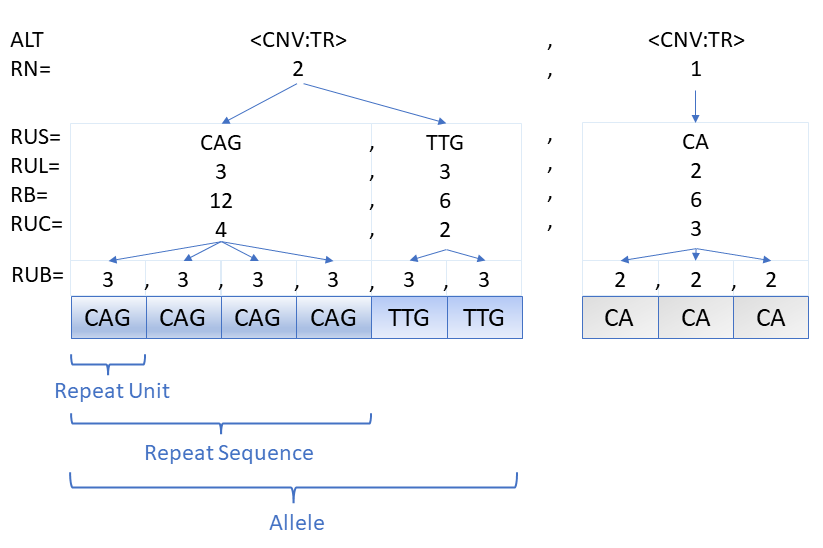
\includegraphics[width=4in,height=2.58in]{img/tandem_repeat_notation.png}
	\caption{$<$CNV:TR$>$ Tandem Repeats}
\end{figure}


A tandem repeat allele can be described by both a $<$CNV:TR$>$ 'summary' record as well as non-symbolic records.
When possible, these records should be phased with their corresponding $<$CNV:TR$>$ record as outlined in the following example.
In the following example, the reference genome contains a $(CAG)_{10}$ repeat at positions 101 to 130 inclusive, the first allele expands this to $(CAG)_{30}$ and the second allele is missing a $G$ from the 6th repeat unit $(CAG)_{5}(CA)_{1}(CAG)_{4}$:

\pagebreak
\footnotesize
\begin{landscape}
\begin{verbatim}
##fileformat=VCFv4.5
##INFO=<ID=SVLEN,Number=A,Type=Integer,Description="Length of structural variant">
##INFO=<ID=CN,Number=A,Type=Float,Description="Copy number of allele">
##INFO=<ID=RN,Number=A,Type=Integer,Description="Total number of repeat sequences in this allele">
##INFO=<ID=RUS,Number=.,Type=String,Description="Repeat unit sequence of the corresponding repeat sequence">
##INFO=<ID=RUL,Number=.,Type=Integer,Description="Repeat unit length of the corresponding repeat sequence">
##INFO=<ID=RUC,Number=.,Type=Float,Description="Repeat unit count of corresponding repeat sequence">
##INFO=<ID=RB,Number=.,Type=Integer,Description="Total number of bases in the corresponding repeat sequence">
##INFO=<ID=CIRUC,Number=.,Type=Float,Description="Confidence interval around RUC">
##INFO=<ID=CIRB,Number=.,Type=Integer,Description="Confidence interval around RB">
##INFO=<ID=RUB,Number=.,Type=Integer,Description="Number of bases in each individual repeat unit">
##FORMAT=<ID=GT,Number=1,Type=String,Description="Genotype">
##FORMAT=<ID=PS,Number=1,Type=Integer,Description="Phase set">
##FORMAT=<ID=CN,Number=1,Type=Float,Description="Copy number">
##ALT=<ID=CNV:TR,Description="Tandem repeat determined based on DNA abundance">
#CHROM POS ID REF ALT QUAL FILTER INFO FORMAT sample
chr1 100 cnv_notation T <CNV:TR>,<CNV:TR> . . SVLEN=30,30;CN=3,0.9666;RUS=CAG,CAG,CA,CAG;RN=1,3;RB=90,15,2,12  GT:PS:CN 1|2:100:3.9666
chr1 117 precise_alt2 AG A . . GT:PS 0|1:100
chr1 130 precise_alt1 G GCAGCAGCAGCAGCAGCAGCAGCAGCAGCAGCAGCAGCAGCAGCAGCAGCAGCAGCAGCAG . . GT:PS 1|0:100
\end{verbatim}
\end{landscape}
\pagebreak
\normalsize

Note the following:
\begin{itemize}
    \item As with all symbolic structural variant alleles, the POS of the $<$CNV:TR$>$ record is the base immediately preceding the tandem repeat
    \item The SVLEN of the $<$CNV:TR$>$ is the length of the reference allele.
    It is not the length of the $<$CNV:TR$>$ allele.
    \item The SVLEN of the $<$CNV:TR$>$ allele of a novel (with respect to the reference) tandem repeat should be 1.
    \item The POS of the $<$CNV:TR$>$ allele of a novel (with respect to the reference) tandem repeat should be the base immediately preceding the inserted tandem repeat sequence.
    \item Both a $<$CNV:TR$>$ and one or more non-symbolic records encoding the tandem repeat can be present.
    \item $<$CNV:TR$>$ and the non-symbolic records encoding the tandem repeat should be phased if possible.
    \item When both $<$CNV:TR$>$ and the equivalent non-symbolic records are present, the $<$CNV:TR$>$ should approximately encode the sequence but is not required to encode the sequence exactly.
	For example, SNVs and indels may be omitted in the $<$CNV:TR$>$ record.
    \item Variant callers which do not report allele-specific tandem repeats should use a single $<$CNV:TR$>$ ALT allele and the missing genotype for the GT field (for example, $./.$ if diploid).
    \item The INFO and FORMAT CN fields should be present for $<$CNV:TR$>$ records (as they are $<$CNV$>$ records) and, when present, must correspond to the sample allelic length divided by the reference allelic length.
	Note that CN FORMAT field represents the overall copy number and the INFO CN the allele-specific copy number.
    \item When benchmarking tandem repeats, the $<$CNV:TR$>$ interval provides a region over which a set of (preferably phased) non-symbolic records can be compared against for length and sequence composition.
    \item RN encodes the number of records for each allele in the RUS, RUL, RUC, RB fields.
	Conceptually, this a mechanism to encode a list-of-list with flat list format used in VCF.
    \item STRs should use RUS, whereas VNTRs should use RUL to ensure the VCF records are not excessively large.
    \item RUL should be omitted when RUS is present (as it is redundant when RS is present).
    \item RUS or RUL must be specified for each $<$CNV:TR$>$.
    \item Support for multiple levels of repeat nesting (such as STRs within VNTRs) is limited to the RUL repeat unit length field which allows the overall length of each top-level repeat unit to be encoded.
    \item The POS and SVLEN of $<$CNV:TR$>$ records should match the STR/VNTR reference catalog sizes for catalog-based callers.
    \item Variant normalisation has limited utility in regions of low complexity as almost identical haplotypes can have very different normalised representations.
\end{itemize}

In some cases, it is desirable to report the full repeat sequence of all alleles at a given repeat locus in a single VCF records.
There are no restrictions on doing so and in the above example, instead of reporting $precise\_alt1$ and $precise\_alt2$, the variants can be represented directly in a single record with a $REF$ of:
\scriptsize
\begin{verbatim}
CAGCAGCAGCAGCAGCAGCAGCAGCAGCAG
\end{verbatim}
\normalsize
and an $ALT$ of:
\scriptsize
\begin{verbatim}
CAGCAGCAGCAGCAGCAGCAGCAGCAGCAGCAGCAGCAGCAGCAGCAGCAGCAGCAGCAGCAGCAGCAGCAGCAGCAGCAGCAGCAGCAG,CAGCAGCAGCAGCAGCACAGCAGCAGCAG
\end{verbatim}
\normalsize

When the length or number of repeat units in a repeat sequence cannot be determined precisely, CIRB and/or CIRUC can be used to define the bounds.
For example, if the total number of $CAG$ repeats at the above locus was at least 50 ($(CAG)_{50-}$) and the mostly likely number of repeats was 65, then the $<$CNV:TR$>$ could be encoded as follows:

\footnotesize
\begin{verbatim}
chr1 100 . T <CNV:TR> . . SVLEN=30;CN=6.5;RUS=CAG;RUC=65;CIRUC=-15,. GT ./.
\end{verbatim}
\normalsize

Note that:
\begin{itemize}
	\item RN was omitted as it is only required if at least one $<$CNV:TR$>$ allele has RN greater than 1.
	\item The confidence interval bounds are relative to the nominal value.
	\item A missing upper bound indicates the maximum length is not known.
\end{itemize}

Exactly representing nested repeats results in the loss of some repeat information when representing with a $<$CNV:TR$>$ record.
For repeats such as $((ACCGGC)_{4}(ACCAGT))_{3-5}$, summarising the repeat structure in a $<$CNV:TR$>$ record requires either unrolling the inner repeats, or treating each outer repeat as a separate repeat sequence (the full repeat structure can be stored in a caller-specific non-standard INFO field).
For many VNTRs, the critical information to retain is the length of each repeat unit.
This length information can be encoded in the RUB field.
For example, a 10,000bp VNTRs domain repeated 5 times, each repeat 500bp longer than the previous can be encoded as follows:

\footnotesize
\begin{verbatim}
chr1 1000000 . T <CNV:TR> . . SVLEN=20000;CN=1.25;RUL=10000;RUC=5;RUB=10000,10500,11000,11500,12000 GT ./.
\end{verbatim}
\normalsize


	
	
\pagebreak
\section{BCF specification}

VCF is very expressive, accommodates multiple samples, and is widely used in the community.
Its biggest drawback is that it is big and slow.
Files are text and therefore require a lot of space on disk.
A normal batch of a hundred exomes is a few GB, but large-scale VCFs with thousands of exome samples quickly become hundreds of GBs.
Because the file is text, it is extremely slow to parse.

Overall, the idea behind is BCF2 is simple.
BCF2 is a binary, compressed equivalent of VCF that can be indexed with tabix and can be efficiently decoded from disk or streams.
For efficiency reasons BCF2 only supports a subset of VCF, in that all info and genotype fields must have their full types specified.
That is, BCF2 requires that if e.g.\ an info field {\tt AC} is present then it must contain an equivalent VCF header line noting that {\tt AC} is an allele indexed array of type integer.

\subsection{Overall file organization}

A BCF2 file is composed of a mandatory header, followed by a series of BGZF compressed blocks of binary BCF2 records.
The BGZF blocks allow BCF2 files to be indexed with tabix.

BGZF blocks are composed of a VCF header with a few additional records and a block of records.
Following the last BGZF BCF2 record block is an empty BGZF block (a block containing zero type of data), indicating that the records are done.

A BCF2 header follows exactly the specification as VCF, with a few extensions/restrictions:
\begin{itemize}
  \item All BCF2 files must have fully specified contigs definitions.
  No record may refer to a contig not present in the header itself.

  \item All INFO and GENOTYPE fields must be fully typed in the BCF2 header to enable type-specific encoding of the fields in records.
  An error must be thrown when converting a VCF to BCF2 when an unknown or not fully specified field is encountered in the records.
\end{itemize}

\subsection{Header}

The BCF2 header contains the following items:

\vspace{0.3cm}
{\small
\begin{tabular}{|l | l | p{30em} | } \hline
\textbf{Field} & \textbf{Type} & \textbf{Notes} \\ \hline
magic          & char[3]     & The characters ``{\tt BCF}'' \\ \hline
major\_version & uint8\_t    & 2 \\ \hline
minor\_version & uint8\_t    & 2 \\ \hline
l\_text        & uint32\_t   & Length of the ``text'' field, including the terminating NUL character \\ \hline
text           & char[l\_text] & VCF format header text, NUL-terminated \\ \hline
\end{tabular}}
\vspace{0.3cm}

The ``magic'' field and version numbers can be used to quickly examine the file to determine that it's a BCF2.2 file.
The ``text'' field contains the standard VCF header lines in text format, from \verb|##fileformat|
to \verb|#CHROM ...| inclusive, terminated by a NUL character.

Because the type is encoded directly in the header, the recommended extension for BCF2 formatted files is {\sl .bcf}.
BCF2 supports encoding values in a dictionary of strings.
The string map is provided by the keyword \verb|##dictionary=S0,S1,...,SN| as a comma-separate ordered list of strings.
See the ``Dictionary of strings'' section for more details.

\subsubsection{Dictionary of strings}

Throughout the BCF file most string values are be specified by integer reference to their dictionary values.
For example, the following VCF record:
\small
\begin{verbatim}
##INFO=<ID=ASP,Number=0,Type=Flag,Description="X">
##INFO=<ID=RSPOS,Number=1,Type=Integer,Description="Y">
##INFO=<ID=dbSNPBuildID,Number=1,Type=Integer,Description="Z">
##contig=<ID=20,length=62435964,assembly=B36,md5=f126cdf8a6e0c7f379d618ff66beb2da,species="Homo sapiens">
#CHROM POS ID REF ALT QUAL FILTER INFO
20 10144 rs144773400 TA T . PASS ASP;RSPOS=10145,dbSNPBuildID=134
20 10228 rs143255646 TA T . PASS ASP;RSPOS=10229;dbSNPBuildID=134
\end{verbatim}
\normalsize
would be encoded inline in BCF2 by reference to the relative position of the header line in the header (ASP=1, RSPOS=2, dbSNPBuildID=3, and PASS implicitly encoded in the first offset PASS=0).

\small
\begin{verbatim}
##INFO=<ID=ASP,Number=0,Type=Flag,Description="X">
##INFO=<ID=RSPOS,Number=1,Type=Integer,Description="Y">
##INFO=<ID=dbSNPBuildID,Number=1,Type=Integer,Description="Z">
##contig=<ID=20,length=62435964,assembly=B36,md5=f126cdf8a6e0c7f379d618ff66beb2da,species="Homo sapiens">
#CHROM POS ID REF ALT QUAL FILTER INFO
0 10144 rs144773400 TA T . s0 s1;s2=10145;s3=134
0 10228 rs143255646 TA T . s0 s1;s2=10229;s3=134
\end{verbatim}
\normalsize

Defined this way, the dictionary of strings depends on the order and the presence of all preceding header lines.
If an existing tag needs to be removed from a BCF, also all consequent tags throughout the whole BCF would have to be recoded.
In order to avoid this costly operation, a new IDX field can be used to explicitly define the position which is dropped on BCF-to-VCF conversion.
If not present, the implicit relative position is assumed.
If the IDX field is present in one record, it must be present also in all other dictionary-defining records.
The IDX tag is not necessary in newly created BCF files, but if present, the numbering must match the implicit dictionary of tags.

Note that the dictionary encoding has the magic prefix `s' here to indicate that the field's value is actually in the dictionary entry giving by the subsequent offset.
This representation isn't actually the one used in BCF2 records but it provides a clean visual guide for the above example.
Note also how the contig has been recoded as a offset into the list of contig declarations.

Note that ``PASS'' is always implicitly encoded as the first entry in the header dictionary.
This is because VCF allows FILTER fields to be PASS without explicitly listing this in the FILTER field itself.


\subsubsection{Dictionary of contigs}

The CHROM field in BCF2 is encoded as an integer offset into the list of \verb|##contig| field headers in the VCF header.
The offsets begin, like the dictionary of strings, at 0.
So for example if in BCF2 the contig value is 10, this indicates that the actual chromosome is the 11th element in the ordered list of \verb|##contig| elements.
Here's a more concrete example:

\small
\begin{verbatim}
##contig=<ID=20,length=62435964,assembly=B36,md5=f126cdf8a6e0c7f379d618ff66beb2da,species="Homo sapiens">
##contig=<ID=21,length=46944323,assembly=B36,md5=f1b74b7f9f4cdbaeb6832ee86cb426c6,species="Homo sapiens">
##contig=<ID=22,length=49691432,assembly=B36,md5=2041e6a0c914b48dd537922cca63acb8,species="Homo sapiens">
#CHROM POS ID REF ALT QUAL FILTER INFO
20 1 . T A . PASS .
21 2 . T A . PASS .
22 3 . T A . PASS .
\end{verbatim}
\normalsize

the actual CHROM field values in the encoded BCF2 records would be 0, 1, and 2 corresponding to the first (offset 0) \verb|##contig| element, etc.

\subsection{BCF2 records}

In BCF2, the original VCF records are converted to binary and encoded as BGZF blocks.
Each record is conceptually two parts.
First is the site information (chr, pos, INFO field).
Immediately after the sites data is the genotype data for every sample in the BCF2 file.
The genotype data may be omitted entirely from the record if there is no genotype data in the VCF file.
Compression of a BCF file is recommended but not required.

\subsubsection{Site encoding}
\label{BcfSiteEncoding}

{\small
\begin{tabular}{|l | l | p{30em} | } \hline
\textbf{Field} &	\textbf{Type} &	\textbf{Notes} \\ \hline
l\_shared & uint32\_t & Data length from CHROM to the end of INFO \\ \hline
l\_indiv  & uint32\_t & Data length of FORMAT and individual genotype fields \\ \hline
CHROM     & int32\_t  & Given as an offset into the mandatory contig dictionary \\ \hline
POS       & int32\_t  & 0-based leftmost coordinate \\ \hline
rlen      & int32\_t  & Length of the record as projected onto the reference sequence.
                        Must be the maximum of the length of the REF allele and the lengths
                        inferred from the SVLEN/LEN of any symbolic alleles \\ \hline
QUAL      & float     & Variant quality; 0x7F800001 for a missing value \\ \hline
n\_info   & uint16\_t & The number of INFO fields in this record \\ \hline
n\_allele & uint16\_t & The number of REF+ALT alleles in this record \\ \hline
n\_sample & uint24\_t & The number of samples in this record, stored as a \textbf{three} byte little-endian value.
                        Note that n\_sample must be equal to the number of samples in the header \\ \hline
n\_fmt    & uint8\_t  & The number of FORMAT keys.  See \ref{GenotypeEncoding} \\ \hline
ID       & typed string & Variant identifier; 0x07 for a missing value \\ \hline
REF+ALT  & list of n\_allele typed strings & the first allele is REF (mandatory) followed by n\_alleles - 1 ALT
                                             alleles, all encoded as typed strings \\ \hline
FILTER   & Typed vector of integers & a vector of integer offsets into dictionary, one for each FILTER field value.
                                      ``.'' is encoded as MISSING \\ \hline
INFO     & field key/value pairs & n\_info pairs of typed vectors.
                                   The first value must be a typed atomic integer giving the offset of the INFO field
                                   key into the dictionary.
                                   The second value is a typed vector giving the value of the field \\ \hline
Genotype values & see below & see below \\ \hline
\end{tabular}}

\subsubsection{Genotype encoding}
\label{GenotypeEncoding}

Genotype fields are encoded not by sample as in VCF but rather by field, with a vector of values for each sample following each field.
In BCF2, the following VCF line:

\vspace{0.3cm}
\begin{tabular}{l l l l}
FORMAT & NA00001 & NA00002 & NA00003 \\
GT:GQ:DP & 0/0:48:1 & 0/1:9:8 & 1/1:43:5 \\
\end{tabular}
\vspace{0.3cm}

would encoded as the equivalent of:

\vspace{0.3cm}
\begin{tabular}{l l l l}
GT=0/0,0/1,1/1 & GQ=48,9,43 & DP=1,8,5
\end{tabular}
\vspace{0.3cm}

Suppose there are i genotype fields in a specific record.
Each i is encoded by a triplet:

BCF2 site information encoding

\vspace{0.3cm}
\small
\begin{tabular}{ | p{2cm} | p{2.5cm} | p{9.5cm} | } \hline
Field & Type & Notes \\ \hline
fmt\_key & typed int & Format key as an offset into the dictionary \\ \hline
fmt\_type & uint8\_t+ & Typing byte of each individual value, possibly followed by a typed int for the vector length.  
In effect this is the same as the typing value for a single vector, but for genotype values it appears only once before the array of genotype field values \\ \hline
\makecell[tl]{fmt\_values \\ (by fmt type)} & Array of values & The information of each individual is concatenated in the vector.  Every value is of the same fmt type.
Variable-length vectors are padded with END\_OF\_VECTOR values; a string is stored as a vector of char \\  \hline
\end{tabular}
\normalsize
\vspace{0.3cm}

The value is always implicitly a vector of N values, where N is the number of samples.
The type byte of the value field indicates the type of each value of the N length vector.
For atomic values this is straightforward (size = 1).
But if the type field indicates that the values are themselves vectors (as often occurs, such as with the PL field) then each of the N values in the outer vector is itself a vector of values.
This encoding is efficient when every value in the genotype field vector has the same length and type.

It is recommended to respect the ordering as specified in the input VCF/BCF2 file, but parsers should not rely on a specific ordering.

If there are no sample records (genotype data) in this VCF/BCF2 file, the size of the genotypes block will be 0.


\subsubsection{Type encoding}
\label{BcfTypeEncoding}

In BCF2 values are all strongly typed in the file.
The type information is encoded in a prefix byte before the value, which contains information about the low-level type of the value(s) such as int32 or float, as well as the number of elements in the value.
The encoding is as follows:

\vspace{0.3cm}
\textbf{BCF2 type descriptor byte}

\vspace{0.3cm}
\begin{tabular}{|p{2cm} | p{10cm}|} \hline
Bit & Meaning \\ \hline
5,6,7,8 bits & The number of elements of the upcoming type. 
For atomic values, the size must be 1. 
If the size is set to 15, this indicates that the vector has 15 or more elements, and that the subsequent BCF2 byte stream contains a typed Integer indicating the true size of the vector. 
If the size is between 2--14, then this Integer is omitted from the stream and the upcoming stream begins immediately with the first value of the vector.
A size of 0 indicates that the value is MISSING. \\ \hline
1,2,3,4 bits & Type \\ \hline
\end{tabular}
\vspace{0.3cm}

The final four bits encodes an unsigned integer that indicates the type of the upcoming value in the data stream.

\textbf{BCF2 types}

\vspace{0.3cm}
\begin{tabular}{|l | l | l|} \hline
Lowest 4 bits & Hexadecimal encoding & Corresponding atomic type \\ \hline
0 & 0x00 & A MISSING value without an explicit type provided \\ \hline
1 & 0x?1 & Integer [8 bit] \\ \hline
2 & 0x?2 & Integer [16 bit] \\ \hline
3 & 0x?3 & Integer [32 bit] \\ \hline
5 & 0x?5 & Float [32 bit] \\ \hline
7 & 0x?7 & Character, ASCII encoded in 8 bits \\ \hline
\end{tabular}
\vspace{0.3cm}

In BCF2 strings are type=7 with an appropriate length.
Single characters are represented as strings with length=1.
Type codes 4,6,8--15 are reserved for future use.

\vspace{0.3cm}

\textbf{Integers} may be encoded as 8, 16, or 32 bit values, in little-endian order.
It is up to the encoder to determine the appropriate ranged value to use when writing the BCF2 file.
For integer types, the values 0x80, 0x8000, 0x80000000 are interpreted as missing values and 0x81, 0x8001, 0x80000001 as END\_OF\_VECTOR indicators (for 8, 16, and 32 bit values, respectively).
Note that the END\_OF\_VECTOR byte is not part of the vector itself and only END\_OF\_VECTOR bytes can follow.
In total, eight values are reserved for future use: 0x80--0x87, 0x8000--0x8007, 0x80000000--0x80000007.

\vspace{0.3cm}
\textbf{Floats} are encoded as single-precision (32 bit) in the basic format defined by the IEEE-754-1985 standard.
This is the standard representation for floating point numbers on modern computers, with direct support in programming languages like C and Java (see Java's Double class for example).
BCF2 supports the full range of values from -Infinity to +Infinity, including NaN.
BCF2 needs to represent missing values for single precision floating point numbers.
This is accomplished by writing the NaN value as the quiet NaN (qNaN), while the MISSING value is encoded as a signaling NaN.
From the NaN wikipedia entry, we have:

\begin{quote}
For example, a bit-wise example of a IEEE floating-point standard single precision (32-bit) NaN would be: s111 1111 1axx xxxx xxxx xxxx xxxx xxxx where s is the sign (most often ignored in applications), a determines the type of NaN, and x is an extra payload (most often ignored in applications).
If a = 1, it is a quiet NaN; if a is zero and the payload is nonzero, then it is a signaling NaN.
\end{quote}

\noindent A good way to understand these values is to play around with the IEEE encoder website.

\vspace{0.3cm}
\noindent Similarly to integers, the float value of 0x7F800001 is interpreted as a MISSING value and 0x7F800002 as the END\_OF\_VECTOR indicator. 
Note that the END\_OF\_VECTOR byte is not part of the vector itself and only END\_OF\_VECTOR bytes can follow.
In total, eight values are reserved for future use:


\vspace{0.1cm}
\begin{tabular}{| l | c | l |} \hline
\textbf{Value}   & \textbf{32-bit precision} & \textbf{Hexadecimal representation} \\ \hline
NaN	    & 0b0111 1111 1100 0000 0000 0000 0000 0000 & 0x7FC00000 \\ \hline
MISSING & 0b0111 1111 1000 0000 0000 0000 0000 0001 & 0x7F800001 \\ \hline
END\_OF\_VECTOR & 0b0111 1111 1000 0000 0000 0000 0000 0010 & 0x7F800002 \\ \hline
reserved & 0b0111 1111 1000 0000 0000 0000 0000 0011 & 0x7F800003 \\ \hline
$\ldots$ & $\ldots$ & $\ldots$ \\ \hline
reserved & 0b0111 1111 1000 0000 0000 0000 0000 0111 & 0x7F800007 \\ \hline
\end{tabular}

\vspace{0.3cm}
\textbf{Character} values are not explicitly typed in BCF2.
Instead, VCF Character values must be encoded by a single character string. See also \ref{character-encoding}.

\vspace{0.3cm}
\textbf{Flags} values --- which can only appear in INFO fields --- in BCF2 should be encoded by any non-reserved value.
The recommended best practice is to encode the value as an 1-element INT8 (type 0x11) with value of 1 to indicate present.
Because FLAG values can only be encoded in INFO fields, BCF2 provides no mechanism to encode FLAG values in genotypes, but could be easily extended to do so if allowed in a future VCF version.

\vspace{0.3cm}
\textbf{String} values have two basic encodings.
For INFO, FORMAT, and FILTER keys these are encoded by integer offsets into the header dictionary.
For string values, such as found in the ID, REF, ALT, INFO, and FORMAT fields, strings are encoded as typed array of ASCII encoded bytes.
The array isn't terminated by a NUL byte.
The length of the string is given by the length of the type descriptor.

Suppose you want to encode the string ``{\tt ACAC}''.
First, we need the type descriptor byte, which is the string type 0x07 or'd with inline size (4) yielding the type byte of 0x40 $|$ 0x07 = 0x47.
Immediately following the type byte is the four byte ASCII encoding of ``{\tt ACAC}'': 0x41 0x43 0x41 0x43.
So the final encoding is:

\vspace{0.1cm}
\begin{tabular}{| l | l |} \hline
0x47 0x41 0x43 0x41 0x43 & String type with inline size of 4 followed by ACAC in ASCII \\ \hline
\end{tabular}
\vspace{0.3cm}

Suppose you want to encode the string ``{\tt VariantCallFormatSampleText}'', a string of size 27.
First, we need the type descriptor byte, which is the string type 0x07.
Because the size exceeds the inline size limit ($27 \geq 15$) we set the size to overflow, yielding the type byte of 0xF0 $|$ 0x07 = 0xF7.
Immediately following the type byte is the typed size of 27, which we encode by the atomic INT8 value: 0x11 followed by the actual size 0x1B.
Finally comes the actual bytes of the string: 0x56 0x61 0x72 0x69 0x61 0x6E 0x74 0x43 0x61 0x6C 0x6C 0x46 0x6F 0x72 0x6D 0x61 0x74 0x53 0x61 0x6D 0x70 0x6C 0x65 0x54 0x65 0x78 0x74.
So the final encoding is:

\vspace{0.3cm}
\begin{tabular}{ | p{9cm} | p{6cm} | } \hline
0xF7 & string with overflow size \\ \hline
0x11 0x1B & overflow size encoded as INT8 with value 27 \\ \hline
0x56 0x61 0x72 0x69 0x61 0x6E 0x74 0x43 0x61 0x6C 0x6C 0x46 0x6F 0x72 0x6D 0x61 0x74 0x53 0x61 0x6D 0x70 0x6C 0x65 0x54 0x65 0x78 0x74 & message in ASCII \\ \hline
\end{tabular}
\vspace{0.3cm}

Suppose you want to encode the missing value `.'.
This is simply a string of size 0 = 0x07.

\vspace{0.3cm}
In VCF there are sometimes fields of type list of strings, such as a number field of unbounded size encoding the amino acid changes due to a mutation.
Since BCF2 doesn't directly support vectors of strings (a vector of character is already a string) we collapse the list of strings into a single comma-separated string, encode it as a regular BCF2 vector of characters, and on reading explode it back into the list of strings.
This works because strings in VCF cannot contain `{\tt ,}' (it's a field separator) and so we can safely use `{\tt ,}' to separate the individual strings.

% String vectors in BCF do not need to start with comma, as the number of
% values is indicated already in the definition of the tag in the header.
%
% For efficiency
% reasons we put a comma at the start of the collapsed string, so that just the
% first character can be examined to determine if the string is collapsed.
%END\_OF\_VECTOR
% To be concrete, suppose we have a info field around X=[A,B,C,D].  This is
% encoded in BCF2 as a single string ``,A,B,C,D'' of size 8, so it would have
% type byte 0x87 followed by the ASCII encoding 0x2C 0x41 0x2C 0x42 0x2C 0x43
% 0x2C 0x44.

\vspace{0.3cm}

\textbf{Vectors} --- The BCF2 type byte may indicate that the upcoming data stream contains not a single value but a fixed length vector of values.
The vector values occur in order (1st, 2nd, 3rd, etc) encoded as expected for the type declared in the vector's type byte.
For example, a vector of 3 16-bit integers would be laid out as first the vector type byte, followed immediately by 3 2-byte values for each integer, including a total of 7 bytes.

Missing values in vectors are handled slightly differently from atomic values.
There are two possibilities for missing values:

One (or more) of the values in the vector may be missing, but others in the vector are not.
Here each value should be represented in the vector, and each corresponding BCF2 vector value either set to its present value or the type equivalent MISSING value.
Alternatively the entire vector of values may be missing.
In this case the correct encoding is as a type byte with size 0 and the appropriate type MISSING.
Suppose we are encoding the record ``AC=[1,2,3]'' from the INFO field.
The AC key is encoded in the standard way.
This would be immediately followed by a typed 8-bit integer vector of size 3, which is encoded by the type descriptor 0x31.
The type descriptor is immediately followed by the three 8-bit integer values: 0x01 0x02 0x03, for a grand total of 4 bytes: 0x31010203.

Suppose we are at a site with many alternative alleles so AC=[1,2,3,4,5,6,7,8,9,10,11,12,13,14,15,16].
Since there are 16 values, we have to use the long vector encoding.
The type of this field is 8 bit integer with the size set to 15 to indicate that the size is the next stream value, so this has type of 0xF1.
The next value in the stream is the size, as a typed 8-bit atomic integer: 0x11 with value 16 0x10.
Each integer AC value is represented by it's value as a 8 bit integer.
The grand total representation here is:

\vspace{0.3cm}
\begin{tabular}{|p{9cm} | p{6cm}|} \hline
0xF1 0x01 0x10 & 8 bit integer vector with overflow size \\ \hline
0x01 0x02 0x03 0x04 0x05 0x06 0x07 0x08 0x09 0x0A 0x0B 0x0C 0x0D 0x0E 0x0F 0x10 & 1--16 as hexadecimal 8 bit integers \\ \hline
\end{tabular}
\vspace{0.3cm}

Suppose this INFO field contains the ``AC=.'', indicating that the AC field is missing from a record with two alt alleles.
The correct representation is as the typed pair of AC followed by a MISSING vector of type 8-bit integer: 0x01.

\vspace{0.3cm}
\textbf{Vectors of mixed length} --- In some cases genotype fields may be vectors whose length differs among samples.  
For example, some CNV call sets encode different numbers of genotype likelihoods for each sample, given the large number of potential copy number states, rather padding all samples to have the same number of fields.  
For example, one sample could have CN0:0,CN1:10 and another CN0:0,CN1:10,CN2:10.  
In the situation when a genotype field contain vector values of different lengths, these are represented in BCF2 by a vector of the maximum length per sample, with all values in the each vector aligned to the left, and END\_OF\_VECTOR values assigned to all values not present in the original vector.  
The BCF2 encoder / decoder must automatically add and remove these END\_OF\_VECTOR values from the vectors. Note that the use of END\_OF\_VECTOR means that it is legal to encode a vector VCF field with MISSING values.

For example, suppose I have two samples, each with a FORMAT field X.  
Sample A has values [1], while sample B has [2,3].  
In BCF2 this would be encoded as [1, END\_OF\_VECTOR] and [2, 3]. 
Diving into the complete details, suppose X is at offset 3 in the dictionary, which is encoded by the typed INT8 descriptor 0x11 followed by the value 0x03. 
Next we have the type of the each format field, which here is a 2 element INT8 vector: 0x21.  
Next we have the encoding for each sample, A = 0x01 0x81 followed by B = 0x02 0x03.  
All together we have:

\vspace{0.3cm}
\begin{tabular}{|p{2cm} | l |} \hline
0x11 0x03 & X dictionary offset \\ \hline
0x21 & each value is a 2 element INT8 value \\ \hline
0x01 0x81 & A is [1, END\_OF\_VECTOR] \\ \hline
0x02 0x03 & B is [2, 3] \\ \hline
\end{tabular}
\vspace{0.3cm}


\vspace{0.3cm}
A \textbf{Genotype (GT) field} is encoded in a typed integer vector (can be 8, 16, or even 32 bit if necessary) with the number of elements equal to the maximum ploidy among all samples at a site.
For one individual, each integer in the vector is organized as $(allele+1) << 1 \mid phased$ where allele is set to $-1$ if the allele in GT is a dot `.' (thus the higher bits are all 0).
The vector is padded with the END\_OF\_VECTOR values if the GT having fewer ploidy.
We note specifically that except for the END\_OF\_VECTOR byte, no other negative values are allowed in the GT array.
When processing VCF version 4.3 or earlier files, the phasing of the first allele should be treated as missing and inferred from the remaining alleles.

Examples:

\vspace{0.3cm}
\small
\begin{tabular}{|p{2.5cm} | p{10cm} | p{3cm}|} \hline
0/1 & in standard format $(0 + 1) << 1 \mid 0$ followed by $(1 + 1) << 1 \mid 0$ & 0x02 04 \\ \hline
0/1, 1/1, and 0/0 & three samples encoded consecutively & 0x02 04 04 04 02 02 \\ \hline
$0\mid1$ & $(1 + 1) << 1 \mid 1$ = 0x05 preceded by the phased first byte value 0x03 & 0x03 05 \\ \hline
./. & where both alleles are missing & 0x00 00 \\ \hline
0 & as an implicitly phased haploid it is represented by a single byte & 0x03 \\ \hline
1 & as an implicitly phased haploid it is represented by a single byte & 0x05 \\ \hline
0/1/2 & is tetraploid, with alleles & 0x02 04 06 \\ \hline
$0/1\mid2$ & is tetraploid with a single phased allele & 0x02 04 07 \\ \hline
0 and 0/1 & pad out the final allele for the haploid individual & 0x02 81 02 04\\ \hline
\end{tabular}
\normalsize

\vspace{0.3cm}
The final example is something seen on chrX when we have a haploid male and a diploid female.
The male genotype vector is terminated prematurely by the END\_OF\_VECTOR value.
\vspace{0.3cm}


\subsection{Encoding a VCF record example}

Let's encode a realistic (but made-up) VCF record.
This is a A/C SNP in HM3 (not really) called in~3 samples.
In this section we'll build up the BCF2 encoding for this record.
\scriptsize
\begin{verbatim}
#CHROM POS ID REF ALT QUAL FILTER INFO FORMAT NA00001 NA00002 NA00003
chr1 101 rs123 A C 30.1 PASS HM3;AC=3;AN=6;AA=C GT:GQ:DP:AD:PL 0/0:10:32:32,0:0,10,100 0/1:10:48:32,16:10,0,100 1/1:10:64:0,64:100,10,0
\end{verbatim}
\normalsize

\subsubsection{Encoding CHROM and POS}

First, let's assume that {\tt chr1} is the second chromosome to appear in the contig list---right after {\tt chrM} ({\tt MT}).
So its offset is 1.
The {\tt POS} BCF2 field value is~101 (obviously).
Because these are both typed values in the BCF2 record, we encode both in their most compact 8-bit value form.
The type byte for an atomic 8-bit integer is 0x11.
The value for the contig offset is 1 = 0x01.
The value 101 is encoded as the single byte 0x65.
So in total these are represented as:

\vspace{0.3cm}
\begin{tabular}{|l | l|} \hline
0x01000000 & CHROM offset is at 1 in 32 bit little endian \\ \hline
0x64000000 & POS in 0 base 32 bit little endian \\ \hline
0x01000000 & rlen = 1 (it's just a SNP) \\ \hline
\end{tabular}

\subsubsection{Encoding QUAL}

The QUAL field value is 30.1, which we encode as an untyped single precision 32-bit float:

\vspace{0.3cm}
\begin{tabular}{|l| l|} \hline
0x41 0xF0 0xCC 0xCD & QUAL = 30.1 as 32-bit float \\ \hline
\end{tabular}

\subsubsection{Encoding ID}

This ID value is a 5-element string, so is encoded as type descriptor 0x57 followed by the five bytes for the string of {\tt 0x72 0x73 0x31 0x32 0x33}.
The full encoding is:

\vspace{0.3cm}
\begin{tabular}{|l| l|} \hline
0x57 0x72 0x73 0x31 0x32 0x33 & ID = rs123 \\ \hline
\end{tabular}

\subsubsection{Encoding REF/ALT fields}

We encode each of REF and ALT as typed strings, first REF followed immediately by ALT.
Each is a 1 element string (0x17), which would then be followed by the single bytes for the bases of 0x43 and 0x41:

\vspace{0.3cm}
\begin{tabular}{|l| l|} \hline
0x17 0x41 & REF A \\ \hline
0x17 0x43 & ALT C \\ \hline
\end{tabular}

\vspace{0.3cm}
Just for discussion, suppose instead that ALT was ALT=C,T.
The only thing that could change is that there would be another typed string following immediately after C encoding 0x17 (1 element string) with the value of 0x54.

\subsubsection{Encoding FILTER}

``PASS'' is implicitly encoded as the first entry in the header dictionary (see dictionary of strings).
Here we encode the PASS FILTER field as a vector of size 1 of type 8-bit, which has type byte is 0x11.
The value is the offset 0:

\vspace{0.3cm}
\begin{tabular}{|l| l|} \hline
0x11 0x00 & FILTER field PASS \\ \hline
\end{tabular}

\subsubsection{Encoding the INFO fields}

HM3;AC=3;AN=6;AA=C
Let's assume that the header dictionary elements for HM3, AC, AN, and AA are at 80, 81, 82, and 83 respectively.
All of these can be encoded by 1-element INT8 values (0x11), with associated hex values of 0x50, 0x51, 0x52, and 0x53 respectively.

First is HM3.
The entry begins with the key: 0x11 0x50.
The HM3 field is a flag with no associated value and therefore the rest of the entry is the special case of a missing value without an explicit type provided.
Altogether we have:

\vspace{0.3cm}
\begin{tabular}{|l| l|} \hline
0x11 0x50 0x00 & HM3 flag is present \\ \hline
\end{tabular}
\vspace{0.3cm}

Now let's encode the two atomic 8-bit integer fields AC and AN:

\vspace{0.3cm}
\begin{tabular}{|l| l|} \hline
0x11 0x51 & AC key \\ \hline
0x11 0x03 & with value of 3 \\ \hline
0x11 0x52 & AN key \\ \hline
0x11 0x06 & with value of 6 \\ \hline
\end{tabular}
\vspace{0.3cm}

The ancestral allele (AA) tell us that among other primates the original allele is C, a Character here.
Because we represent Characters as single element strings in BCF2 (0x17) with value 0x43 (C).
So the entire key/value pair is:

\vspace{0.3cm}
\begin{tabular}{|l |l|} \hline
0x11 0x53 & AA key \\ \hline
0x17 0x43 & with value of C \\ \hline
\end{tabular}

\subsubsection{Encoding Genotypes}

Continuing with our example:

\vspace{0.3cm}
\begin{tabular}{l l l l}
FORMAT & NA00001 & NA00002 & NA00003 \\
GT:GQ:DP:AD:PL & 0/0:10:32:32,0:0,10,100 & 0/1:10:48:32,16:10,0,100 & 1/1:10:64:0,64:100,10,0 \\
\end{tabular}
\vspace{0.3cm}

Here we have the specially encoded GT field.
We have two integer fields GQ and DP.
We have the AD field, which is a vector of 2 values per sample.
And finally we have the PL field which is 3 values per sample.
Let's say that the FORMAT keys for GT, GQ, DP, AD, and PL are at offsets 1, 2, 3, and 4, 5, respectively.
Now let's encode each of the genotype fields in order of the VCF record (GT, GQ, DP, AD, and then PL):

GT triplet begins with the key: 0x1101.
Next is the type of the field, which will be a 2-element (diploid) INT8 type: 0x21.
This is followed by 3 2-byte arrays of values 0x0202 0x0204 0x0404 (see genotype encoding example for details).
The final encoding is 0x1101 0x21 0x020202040404

GQ triplet begins with the key 0x1102.
Because these values are small, we encode them as 8 bit atomic integers with type code 0x11.
As each value is the same (10 = 0x0A) the GQ field is encoded as 0x1102 0x11 0x0A0A0A

DP almost identical to GQ.
First is the 0x1103 key, followed by 3 8-bit atomic integers encoded as 0x11 (the type) 0x20 (DP=32), 0x30 (DP=48) and 0x40 (DP=64).
So we have: 0x1103 0x11203040

AD is more complex.
The key is simple, just like the others, with 0x1104.
Because the AD field is a vector of 2 values for each genotype, the value of key/value pair a vector type.
Because the integer values in each AD field of each sample are small they are encoded by 8 bit values.
So the value type is = 0x21.
For sample one there are two values: 32,0 which are 0x30 and 0x00.
Samples two and three are 0x30 0x20 and 0x00 0x40 respectively.
So ultimately this field is encoded as 0x1104 0x21 0x300030200040

PL is just like AD but with three values per sample.
The key is 0x1105.
Because the PL field is a vector of 3 values for each genotype, the value of key/value pair a vector type, and because the size is 3 it's encoded in the size field of the type.
Again, because the integer values in each PL field of each sample are small they are encoded by 8 bit values.
So the value type 0x31.
For sample one there are three values: 0, 10, and 100 which are 0x00, 0x0A, and 0x64.
Samples two and three have the same values but in a slightly different order.
So ultimately the PL field is encoded as 0x1105 0x31 0x000A64 0x0A0064 0x640A00

So the genotype block contains:

\vspace{0.3cm}
\begin{tabular}{|l| l|} \hline
0x1101 0x21 0x020202040404 & GT \\ \hline
0x1102 0x11 0x0A0A0A & GQ \\ \hline
0x1103 0x11 0x203040 & DP \\ \hline
0x1104 0x21 0x300030200040 & AD \\ \hline
0x1105 0x31 0x000A640A0064640A00 & PL \\ \hline
\end{tabular}
\vspace{0.3cm}

\textbf{Putting it all together}

We need to determine a few values before writing out the final block:

l\_shared = 51 (Data length from CHROM to the end of INFO)

l\_indiv = 42 (Data length of FORMAT and individual genotype fields)

n\_info = 4 (Number of INFO fields)

n\_allele = 2 (Number of alleles, including REF)

n\_sample = 3 (Number of samples)

n\_fmt = 5 (Number of FORMAT keys)

\vspace{0.3cm}
\begin{tabular}{|l| l|} \hline
0x33000000 & l\_shared as 32-bit little endian hex \\ \hline
0x2A000000 & l\_indiv as 32-bit little endian hex \\ \hline
0x01000000 & CHROM offset is at 1 in 32 bit little endian \\ \hline
0x64000000 & POS in 0-based 32-bit little endian \\ \hline
0x01000000 & rlen = 1 (it's just a SNP) \\ \hline
0x41 0xF0 0xCC 0xCD & QUAL = 30.1 as 32-bit float \\ \hline
0x0400     & n\_info as 16-bit little-endian \\ \hline
0x0200     & n\_allele as 16-bit little-endian \\ \hline
0x030000   & n\_sample as 24-bit little-endian \\ \hline
0x05       & n\_fmt \\ \hline
0x57 0x72 0x73 0x31 0x32 0x33 & ID = rs123 \\ \hline
0x17 0x41 & REF A \\ \hline
0x17 0x43 & ALT C \\ \hline
0x11 0x00 & FILTER field PASS \\ \hline
0x11 0x50 0x00 & HM3 flag is present \\ \hline
0x11 0x51 & AC key \\ \hline
0x11 0x03 & with value of 3 \\ \hline
0x11 0x52 & AN key \\ \hline
0x11 0x06 & with value of 6 \\ \hline
0x11 0x53 & AA key \\ \hline
0x17 0x43 & with value of C \\ \hline
0x1101 0x21 0x020202040404 & GT \\ \hline
0x1102 0x11 0x0A0A0A & GQ \\ \hline
0x1103 0x11 0x203040 & DP \\ \hline
0x1104 0x21 0x300030200040 & AD \\ \hline
0x1105 0x31 0x000A640A0064640A00 & PL \\ \hline
\end{tabular}
\vspace{0.3cm}

That's quite a lot of information encoded in only 96 bytes!

\subsection{BCF2 block gzip and indexing}

These raw binary records may be subsequently encoded into BGZF blocks following the BGZF compression format, section 3 of the SAM format specification.
BCF2 records can be raw, though, in cases where the decoding/encoding costs of bgzipping the data make it reasonable to process the data uncompressed, such as streaming BCF2s through pipes with samtools and bcftools.
Here the files should be still compressed with BGZF but with compression 0.
Implementations should perform BGZF encoding and must support the reading of both raw and BGZF encoded BCF2 files.

BCF2 files are expected to be indexed through the same index scheme, section~4 as BAM files and other block-compressed files with BGZF.

\section{List of changes}

\subsection{Changes between VCFv4.5 and VCFv4.4}

\begin{itemize}
	\item Added base modification support (FORMAT M5mC, M5hmC, M6mA, etc.).
	\item Reserved all FORMAT keys of the form $M[0-9]+$ as base modification fields.
	\item Added Number=P support for fields with cardinality matching sample ploidy/local copy number.
	\item Added local allele support (Number=LA, LG, LR; FORMAT LAA, LAD, LADF, LADR, LEC, LGL, LGP, LPL, LPP) to reduce the size of multi-sample VCFs and enable lossless merging.
	\item Deprecated INFO END. It is now a computed field written only for backwards compatibility with older versions of VCF.
	\item Updated BCF rlen field to reflect INFO END being a computed value.
	\item Added FORMAT LEN to support sample-specific $<$*$>$ alleles.
	\item Clarified that the header line is indeed mandatory
	\item Clarified that $<$NON\_REF$>$ should be treated as an alias of $<$*$>$
\end{itemize}

\subsection{VCFv4.4 Errata}

\begin{itemize}
	\item Type=P added to FORMAT field type list (used by PSL/PSO fields)
\end{itemize}

\subsection{Changes between VCFv4.4 and VCFv4.3}

\begin{itemize}
\item Added tandem repeat support ($<$CNV:TR$>$, RN, RUS, RUL, RB, CIRB, RUC, CIRUC, RUB)
\item Redefined INFO CN as allele-specific copy number and FORMAT CN as total copy number.
\item Redefined INFO and FORMAT CN to support non-integer copy numbers.
\item Added support for phasing and derivative chromosome reconstruction in the presence of SVs (PSL, PSO, PSQ)
\item Added SVCLAIM to disambiguate copy number based $<$DEL$>$ and $<$DUP$>$ variants from breakpoint based ones.
\item Conceptually separated variant detection and interpretation.
\item Added EVENTTYPE/EVENT to enable the multiple records encoding complex genomic rearrangements to be grouped together.
\item Added polyploid partial phasing support (e.g. GT $|0|0/1/2$). GT now defined as a prefix notation with the first phasing indicator optional.
\item Redefined $Number=$ for SVLEN, CIPOS, CIEND, HOMLEN, HOMSEQ, BKPTID, MEINFO, METRANS, DGVID, DBVARID, DBRIPID, MATEID, PARID, EVENT, CN, CICN to support multiple symbolic alleles.
\item Redefined END as the end position of the longest ALT allele. Note that END remains $Number=1$.
\item Redefined SVLEN to always be positive and be meaningful for INV variants.
\item Redefined SVLEN, END and BCF rlen to support both $<*>$ and symbolic structural variant alleles in the same record.
\item Number, Type and Description required only for INFO meta-information lines
\item Clarified CIPOS should be used to define micro-homology bounds
\item Clarified INFO lines field ordering
\item Clarified that symbolic and breakpoint notation ALT alleles are case sensitive.
\item Deprecated SVTYPE
\item Removed DPADJ, CNADJ, CICNADJ
\item Disallowed BND ALT records (these should use breakpoint notation anyway)
\item Removed definition of DP from Section 3 as it was already defined in Section 1.6.1.8.
\item Deprecated bundles in favour of PSL-based phasing.
\item Updated SV examples.
\item BCF parsers should perform BGZF encoding and must support both raw and BGZF encoded files.
\end{itemize}

\subsection{Changes to VCFv4.3}

\begin{itemize}
\item More strict language: ``should'' replaced with ``must'' where appropriate
\item Tables with Type and Number definitions for INFO and FORMAT reserved keys

\item
The set of characters allowed in VCF contig names is now the same as that allowed in SAM reference sequence names, which was restricted in January 2019.
The characters `{\tt\verb|\|\,,\,"`'\,()\,\verb|{}|}' are now invalid in VCF contig names, while `{\tt *}' is now valid when not the first character.
(The characters `{\tt []\,<>}' and initial~`{\tt *}'/`{\tt =}' were already invalid and remain so.)

The VCF specification previously disallowed colons (`{\tt :}') in contig names to avoid confusion when parsing breakends, but this was unnecessary.
Even with contig names containing colons, the breakend mate position notation can be unambiguously parsed because the ``{\tt :}\emph{pos}'' part is \textbf{always} present.
\item Added PP tag which is the phred-scaled analogue to GP
\end{itemize}

\subsection{Changes between VCFv4.2 and VCFv4.3}

\begin{itemize}
\item VCF compliant implementations must support both LF and CR+LF newline conventions
\item INFO and FORMAT tag names must match the regular expression \texttt{\^{}[A-Za-z\_][0-9A-Za-z\_.]*\$}
\item Spaces are allowed in INFO field values
\item Characters with special meaning (such as `;' in INFO, `:' in FORMAT, and `\%' in both) can be encoded using percent encoding (see Section~\ref{character-encoding})
\item The character encoding of VCF files is UTF-8.
\item The SAMPLE field can contain optional DOI URL for the source data file
\item Introduced \#\#META header lines for defining phenotype metadata
\item New reserved tag ``CNP'' analogous to ``GP'' was added. Both CNP and GP use 0 to 1 encoding, which is a change from previous phred-scaled GP.
\item In order for VCF and BCF to have the same expressive power, we state explicitly that Integers and Floats are 32-bit numbers.
Integers are signed.
\item We state explicitly that zero length strings are not allowed, this includes the CHROM and ID column, INFO IDs, FILTER IDs and FORMAT IDs.
Meta-information lines can be in any order, with the exception of \#\#fileformat which must come first. 
\item All header  lines of the form \#\#key=$<$ID=xxx,...$>$ must have an ID value that is unique for a given value of ``key''.
All header lines whose value starts with ``$<$'' must have an ID field.
Therefore, also \#\#PEDIGREE newly requires a unique ID.
\item We state explicitly that duplicate IDs, FILTER, INFO or FORMAT keys are not valid.
\item A section about gVCF was added, introduced the $<$*$>$ symbolic allele.
\item A section about tag naming conventions was added.
\item New reserved AD, ADF, and ADR INFO and FORMAT fields added.
\item Removed unused and ill-defined GLE FORMAT tag.
\item Chromosome names cannot use reserved symbolic alleles and contain characters used by breakpoints (Section~\ref{sec-contig-field}).
\item IUPAC ambiguity codes should be converted to a concrete base.
\item Symbolic ALTs for IUPAC codes.
\end{itemize}

\subsection{Changes between BCFv2.1 and BCFv2.2}
\begin{itemize}
\item BCF header lines can include optional IDX field
\item We introduce END\_OF\_VECTOR byte and reserve 8 values for future use
\item Clarified that except the END\_OF\_VECTOR byte, no other negative values are allowed in the GT array 
\item String vectors in BCF do not need to start with comma, as the number of values is indicated already in the definition of the tag in the header.
\item The implicit filter PASS was described inconsistently throughout BCFv2.1: It is encoded as the first entry in the dictionary, not the last.
\end{itemize}

\subsection{Changes between VCFv4.1 and VCFv4.2}
\begin{itemize}
\item In the HEADER the INFO definition allow additional field after the 4 first mandatory fields
\item INFO fields definition can use Number=R to specify one per allele including the reference.
\item Allow star allele in the ALT for describing upstream deletion
\end{itemize}

\end{document}

\title{The Variant Call Format Specification \\ \vspace{0.5em} \large VCFv4.5 and BCFv2.2}
\date{\headdate}
\maketitle
\begin{quote}\small
The master version of this document can be found at \url{https://github.com/samtools/hts-specs}.\\
This printing is version~\commitdesc\ from that repository, last modified on the date shown above.
\end{quote}
\vspace*{1em}

\newpage
\tableofcontents
\newpage

\section{The VCF specification}
VCF is a text file format (most likely stored in a compressed manner).
It contains meta-information lines (prefixed with ``\verb|##|''), a header line (prefixed with ``\verb|#|''), and data lines each containing information about a position in the genome and genotype information on samples for each position (text fields separated by tabs).
Zero length fields are not allowed, a dot (``.'') must be used instead.
In order to ensure interoperability across platforms, VCF compliant implementations must support both LF (``\verb|\n|'') and CR+LF (``\verb|\r\n|'') newline conventions.

\subsection{An example}
\scriptsize
\begin{verbatim}
##fileformat=VCFv4.5
##fileDate=20090805
##source=myImputationProgramV3.1
##reference=file:///seq/references/1000GenomesPilot-NCBI36.fasta
##contig=<ID=20,length=62435964,assembly=B36,md5=f126cdf8a6e0c7f379d618ff66beb2da,species="Homo sapiens",taxonomy=x>
##phasing=partial
##INFO=<ID=NS,Number=1,Type=Integer,Description="Number of Samples With Data">
##INFO=<ID=DP,Number=1,Type=Integer,Description="Total Depth">
##INFO=<ID=AF,Number=A,Type=Float,Description="Allele Frequency">
##INFO=<ID=AA,Number=1,Type=String,Description="Ancestral Allele">
##INFO=<ID=DB,Number=0,Type=Flag,Description="dbSNP membership, build 129">
##INFO=<ID=H2,Number=0,Type=Flag,Description="HapMap2 membership">
##FILTER=<ID=q10,Description="Quality below 10">
##FILTER=<ID=s50,Description="Less than 50% of samples have data">
##FORMAT=<ID=GT,Number=1,Type=String,Description="Genotype">
##FORMAT=<ID=GQ,Number=1,Type=Integer,Description="Genotype Quality">
##FORMAT=<ID=DP,Number=1,Type=Integer,Description="Read Depth">
##FORMAT=<ID=HQ,Number=2,Type=Integer,Description="Haplotype Quality">
#CHROM POS     ID        REF    ALT     QUAL FILTER INFO                              FORMAT      NA00001        NA00002        NA00003
20     14370   rs6054257 G      A       29   PASS   NS=3;DP=14;AF=0.5;DB;H2           GT:GQ:DP:HQ 0|0:48:1:51,51 1|0:48:8:51,51 1/1:43:5:.,.
20     17330   .         T      A       3    q10    NS=3;DP=11;AF=0.017               GT:GQ:DP:HQ 0|0:49:3:58,50 0|1:3:5:65,3   0/0:41:3
20     1110696 rs6040355 A      G,T     67   PASS   NS=2;DP=10;AF=0.333,0.667;AA=T;DB GT:GQ:DP:HQ 1|2:21:6:23,27 2|1:2:0:18,2   2/2:35:4
20     1230237 .         T      .       47   PASS   NS=3;DP=13;AA=T                   GT:GQ:DP:HQ 0|0:54:7:56,60 0|0:48:4:51,51 0/0:61:2
20     1234567 microsat1 GTC    G,GTCT  50   PASS   NS=3;DP=9;AA=G                    GT:GQ:DP    0/1:35:4       0/2:17:2       1/1:40:3
\end{verbatim}
\normalsize
This example shows (in order): a good simple SNP, a possible SNP that has been filtered out because its quality is below 10, a site at which two alternate alleles are called, with one of them (T) being ancestral (possibly a reference sequencing error), a site that is called monomorphic reference (i.e.\ with no alternate alleles), and a microsatellite with two alternative alleles, one a deletion of 2 bases (TC), and the other an insertion of one base (T).
Genotype data are given for three samples, two of which are phased and the third unphased, with per sample genotype quality, depth and haplotype qualities (the latter only for the phased samples) given as well as the genotypes.
The microsatellite calls are unphased.

\subsection{Character encoding, non-printable characters and characters with special meaning}
\label{character-encoding}
The character encoding of VCF files is UTF-8.
UTF-8 is a multi-byte character encoding that is a strict superset of 7-bit ASCII and has the property that none of the bytes in any multi-byte characters are 7-bit ASCII bytes.
As a result, most software that processes VCF files does not have to be aware of the possible presence of multi-byte UTF-8 characters.
VCF files must not contain a byte order mark.
Note that non-printable characters U+0000--U+0008, U+000B--U+000C, U+000E--U+001F are disallowed.
Line separators must be CR+LF or LF and they are allowed only as line separators at end of line.
Some characters have a special meaning when they appear (such as field delimiters `\verb|;|' in INFO or `\verb|:|' FORMAT fields), and for any other meaning they must be represented with the capitalized percent encoding:

\begingroup\footnotesize
\begin{tabular}{l l l}
\%3A  &  :  & (colon)                \\
\%3B  &  ;  & (semicolon)            \\
\%3D  &  =  & (equal sign)           \\
\%25  &  \% & (percent sign)         \\
\%2C  &  ,  & (comma)                \\
\%0D  & CR  &                        \\
\%0A  & LF  &                        \\
\%09  & TAB & 
\end{tabular}
\endgroup


\subsection{Data types}
Data types supported by VCF are: Integer (32-bit, signed), Float (32-bit IEEE-754, formatted to match one of the regular expressions \verb|^[-+]?[0-9]*\.?[0-9]+([eE][-+]?[0-9]+)?$| or \verb"^[-+]?(INF|INFINITY|NAN)$" case insensitively),%
\footnote{Note Java's {\tt Double.valueOf} is particular about capitalisation, so additional code is needed to parse all VCF infinite/NaN values.}
Flag, Character, and String.
For the Integer type, the values from $-2^{31}$ to $-2^{31}+7$ cannot be stored in the binary version and therefore are disallowed in both VCF and BCF, see \ref{BcfTypeEncoding}.

\subsection{Meta-information lines}
File meta-information lines start with ``\verb|##|'' and must appear first in the VCF file, before the header line (section~\ref{header-line}) and data record lines (section~\ref{data-lines}).
They may be either \emph{unstructured} or \emph{structured}.

An \emph{unstructured} meta-information line consists of a~\emph{key} (denoting the type of meta-information recorded) and a~\emph{value} (which may not be empty and must not start with a `\verb|<|' character), separated by an `\verb|=|' character:
\begin{quote}
\verb|##|\emph{key}\verb|=|\emph{value}
\end{quote}
Several unstructured meta-information lines are defined in this specification, notably \verb|##fileformat|.
Others not defined by this specification, e.g.\ \verb|##fileDate| and \verb|##source|, are commonly found in VCF files.
These typically have meanings that are obvious, or they are immaterial for processing the file, or both.

A \emph{structured} meta-information line is similar, but the value is itself a comma-separated list of key=value pairs, enclosed within `\verb|<|' and `\verb|>|' characters:
\begin{quote}
\verb|##|\emph{key}\verb|=<|\emph{key}\verb|=|\emph{value}\verb|,|\emph{key}\verb|=|\emph{value}\verb|,|\emph{key}\verb|=|\emph{value}\verb|,|\ldots\verb|>|
\end{quote}
All structured lines require an ID which must be unique within their type, i.e., within all the meta-information lines with the same ``\verb|##|\emph{key}\verb|=|'' prefix.
For all of the structured lines (\verb|##INFO|, \verb|##FORMAT|, \verb|##FILTER|, etc.) described in this specification, optional fields can be included.
For example:
\begin{verbatim}
##INFO=<ID=ALLELEID,Number=A,Type=String,Description="Allele ID",Source="ClinVar",Version="20220804">
\end{verbatim}
In the above example, the optional fields of ``Source'' and ``Version'' are provided.
The values of optional fields must be written as quoted strings, even for numeric values.
Other structured lines not defined by this specification may also be used; the only required field for such lines is the required \verb|ID| field.

It is recommended in VCF and required in BCF that the header includes tags describing the reference and contigs backing the data contained in the file.
These tags are based on the SQ field from the SAM spec; all tags are optional (see the VCF example above).

To aid human readability, the order of fields should be ID, Number, Type, Description, then any optional fields.
Implementations must not rely on the order of the fields within structured lines and are not required to preserve field ordering.

Meta-information lines are optional, but if they are present then they must be completely well-formed.
Other than \verb|##fileformat|, they may appear in any order.
Note that BCF, the binary counterpart of VCF, requires that all entries are present.
It is recommended to include meta-information lines describing the entries used in the body of the VCF file.


\subsubsection{File format}
A single `fileformat' line is always required, must be the first line in the file, and details the VCF format version number.
For VCF version 4.5, this line is:

\begin{verbatim}
##fileformat=VCFv4.5
\end{verbatim}


\subsubsection{Information field format}
INFO meta-information lines are structured lines with required fields ID, Number, Type, and Description, and recommended optional fields Source and Version:

\begin{verbatim}
##INFO=<ID=ID,Number=number,Type=type,Description="description",Source="source",Version="version">
\end{verbatim}

Possible Types for INFO fields are: Integer, Float, Flag, Character, and String.
The Number entry is an Integer that describes the number of values that can be included with the INFO field.
For example, if the INFO field contains a single number, then this value must be $1$; if the INFO field describes a pair of numbers, then this value must be $2$ and so on.
There are also certain special characters used to define special cases:

\begin{itemize}
  \item A: The field has one value per alternate allele.
  The values must be in the same order as listed in the ALT column (described in section \ref{data-lines}).
  \item R: The field has one value for each possible allele, including the reference.
  The order of the values must be the reference allele first, then the alternate alleles as listed in the ALT column.
  \item G: The field has one value for each possible genotype.
  The values must be in the same order as prescribed in section \ref{genotype-fields:genotype-ordering} (see \textsc{Genotype Ordering}).
  \item . (dot): The number of possible values varies, is unknown or unbounded.
\end{itemize}

The `Flag' type indicates that the INFO field does not contain a Value entry, and hence the Number must be $0$ in this case.
The Description value must be surrounded by double-quotes.
Double-quote character must be escaped with backslash $\backslash$ and backslash as $\backslash\backslash$.
Source and Version values likewise must be surrounded by double-quotes and specify the annotation source (case-insensitive, e.g.\ \verb|"dbsnp"|) and exact version (e.g.\ \verb|"138"|), respectively for computational use.

\subsubsection{Filter field format}
FILTER meta-information lines are structured lines with required fields ID and Description that define the possible content of the FILTER column in the VCF records:

\begin{verbatim}
##FILTER=<ID=ID,Description="description">
\end{verbatim}

\subsubsection{Individual format field format}
FORMAT meta-information lines are structured lines with required fields ID, Number, Type, and Description that define the possible content of the per-sample/genotype columns in the VCF records:

\begin{verbatim}
##FORMAT=<ID=ID,Number=number,Type=type,Description="description">
\end{verbatim}

Possible Types for FORMAT fields are: Integer, Float, Character, and String (this field is otherwise defined precisely as the INFO field).
The Number field is defined as per the INFO Number field with the following additional possibilities:

\begin{itemize}
  \item LA: Identical to A except the only alternate alleles defined in the $LAA$ field are considered present.
  \item LR: Identical to R except the only alternate alleles defined in the $LAA$ field are considered present.
  \item LG: Identical to G except the only alternate alleles defined in the $LAA$ field are considered present.
  \item P: The field has one value for each allele value defined in $GT$.
  \item M: The field has one value for each possible base modification for the corresponding ChEBI ID.
\end{itemize}

The cardinality of M fields is determined by genotype and number of possible base modifications for the corresponding alleles.
The ID of all M fields must end with A, C, G, T, U, or N which defines the base(s) that the modification can occur on.
U must be treated as synonymous with T.
If any base modification key is present for a sample, GT must be defined for that sample.
The number of base modification values for a given allele is the number of bases on either strand in the allele sequence that could contain the base modification.
The order of the base modification values is the order that these bases occur in the allele.
For N base modifications, the field contains values for both the positive and negative strands with the negative strand value immediately after the positive strand value.
For example, an allele of CGA has 2 M5mC values, the first defining the methylation rate on forward strand C at the first base pair, and the second defining the methylation rate for reverse strand C at the second base pair.

The order and number of alleles encoded in these fields is determined by the order and phasing in the genotype.
Base modifications values are encoded in their GT order with one value for each possible base modification in the concatenated genotype allele bases.
Unphased allele values are aggregated and encoded at the position of the first occurrence of the unphased allele value.
MISSING allele values and symbolic alleles are treated as containing no relevant bases thus encode no base modification values.

Unstranded base modification information should be stored at the base with the lowest POS with the other values MISSING.
Unstranded N base modifications should be stored on the positive strand with the values MISSING.
For example, unstranded 5mC CpG methylation should be stored on the VCF recording containing the C with the M5mC value of the subsequent G set to MISSING or omitted entirely. Similarly, unstranded MxaoN values should be stored in the positive strand value with the negative strand value MISSING.

Examples: 

\vspace{0.5em}
\begin{tabular}{ l l l l l l l l l l}
	\#CHROM & POS & REF & ALT & FORMAT & SAMPLE\\
	chr & $10$ & C & A         & GT:M5mC       & \tt{0/1:0.95}\\
	chr & $20$ & C & CTAG      & GT:M5mC       & \tt{0/1:0,0.5,0.7}\\
	chr & $30$ & C & .         & GT:M5mC:M5hmC & \tt{0|0:0.9,0:0,0.1}\\
	chr & $40$ & C & A,T,G,ACG & GT:M5mC       & \tt{/3|1/0|4|0/0/3/1:0.25,0.1,0.5,0.6,.}\\
\end{tabular}

The first record encodes a 95 percent methylation on the REF C.
Since the ALT A cannot be 5mC methylated, only one value is present.

The second record encodes the methylation of the REF (since it's the first allele occurring the GT field), followed by the methylation values of the first and fourth base of the CTAG ALT.

The third record encodes that both 5mC and 5hmC modifications are present at the homozygous C but they are mutually exclusive allele: 90 percent 5mC and no 5hmC on the first haplotype, and 10 percent 5hmC with no 5mC on the second haplotype.

The fourth record demonstrates the encoded ordering of the methylation state of a partially phased locally-octoploid sample.
The first   allele value (unphased G) encodes a 25 percent methylation of the 2 unphased copies of the G allele (encoded first since /3 occurs first in GT).
The second  allele value (phased A)   is not relevant to 5mC methylation so there is nothing to encode.
The third   allele value (unphased C) encodes a 10 precent methylation rate for both unphased copies of the C REF allele.
The fourth  allele value (phased ACG) encoding the 50 and 60 percent methylation rates of the second and third base pairs of the ACG allele.
The fifth   allele value (phased C)   encodes an unknown methylation rate of the single phased copy of the C REF allele.
The sixth   allele value (unphased C) was already encoded as part of the third allele value so there is nothing more to encode.
The seventh allele value (unphased G) was already encoded as part of the first allele value so there is nothing more to encode.
The eighth  allele value (unphased A) is not relevant to 5mC methylation so there is nothing to encode.


\subsubsection{Alternative allele field format} \label{altfield}
ALT meta-information lines are structured lines with require fields of ID and Description that describe the possible symbolic alternate alleles in the ALT column of the VCF records:

\begin{verbatim}
##ALT=<ID=type,Description="description">
\end{verbatim}

\noindent \textbf{Structural Variants} \newline
In symbolic alternate alleles for structural variants, the ID field indicates the type of structural variant, and can be a colon-separated list of types and subtypes.
ID values are case sensitive strings and must not contain whitespace, commas or angle brackets (See \ref{fixed-fields}.\ref{fixed-fields-alt})
The first level type must be one of the following:
\begin{itemize}
  \item DEL Region of lowered copy number relative to the reference, or a deletion breakpoint
  \item INS Insertion of novel sequence relative to the reference
  \item DUP Region of elevated copy number relative to the reference, or a tandem duplication breakpoint
  \item INV Inversion of reference sequence
  \item CNV Region of uniform copy number (may be deletion, duplication or copy number neutral)
\end{itemize}

The CNV symbolic allele should not be used when a more specific one (e.g. DEL, CNV:TR) can be applied.

Implementations are free to define their own subtypes.
The presence of a subtype does not change either the copy number or breakpoint interpretation of a symbolic structural variant allele.
The following subtypes are recommended:
\begin{itemize}
  \item CNV:TR Tandem repeat. See \ref{tandem-repeats} for further details.
  \item DUP:TANDEM Tandem duplication
  \item DEL:ME Deletion of mobile element relative to the reference
  \item INS:ME Insertion of a mobile element relative to the reference
\end{itemize}

Note that the position of symbolic structural variant alleles is the position of the base immediately preceding the variant.

\bigskip

\noindent \textbf{IUPAC ambiguity codes} \newline
Symbolic alleles can be used also to represent genuinely ambiguous data in VCF, for example:
\begin{verbatim}
    ##ALT=<ID=R,Description="IUPAC code R = A/G">
    ##ALT=<ID=M,Description="IUPAC code M = A/C">
\end{verbatim}

\subsubsection{Assembly field format}
Breakpoint assemblies for structural variations may use an external file:
\begin{verbatim}
##assembly=url
\end{verbatim}

The URL field specifies the location of a fasta file containing breakpoint assemblies referenced in the VCF records for structural variants via the BKPTID INFO key.

\subsubsection{Contig field format}
\label{sec-contig-field}
It is recommended for VCF, and required for BCF, that the header includes tags describing the contigs referred to in the file.
The structured \texttt{contig} field must include the ID attribute and can include additional optional attributes with
the following ones reserved:
\begin{itemize}
  \item length: the length of the sequence
  \item md5: MD5 checksum of the sequence as defined in the Sam specification v1\footnote{See Reference MD5 calculation
      section in \href{https://samtools.github.io/hts-specs/SAMv1.pdf}{\tt SAM Format Specification}.} Briefly, the digest
      is calculated excluding all characters outside of the inclusive range 33 (`\char33') to 126 (`\char126').
      and all lowercase characters converted to uppercase. The MD5 digest is calculated as described in
      \href{https://tools.ietf.org/html/rfc1321}{\sl RFC 1321} and presented as a 32 character lowercase hexadecimal number.
  \item URL: tag to indicate where the sequence can be found
\end{itemize}

For example:
{\scriptsize
\begin{verbatim}
##contig=<ID=ctg1,length=81195210,URL=ftp://somewhere.example/assembly.fa,md5=f126cdf8a6e0c7f379d618ff66beb2da,...>
\end{verbatim}
}
\noindent
Contig names follow the same rules as the SAM format's reference sequence names:
they may contain any printable ASCII characters in the range \verb|[!-~]| apart from `{\tt\verb|\|\,,\,"`'\,()\,[]\,\verb|{}|\,<>}' and may not start with `{\tt *}' or `{\tt =}'.
Thus they match the following regular expression:
\begin{verbatim}
    [0-9A-Za-z!#$%&+./:;?@^_|~-][0-9A-Za-z!#$%&*+./:;=?@^_|~-]*
\end{verbatim}
\noindent
In particular, excluding commas facilitates parsing \verb|##contig| lines, and excluding the characters `\verb|<>[]|' and initial~`{\tt *}' avoids clashes with symbolic alleles.
The contig names must not use a reserved symbolic allele name.


\subsubsection{Sample field format}
It is possible to define sample to genome mappings as shown below:
{\scriptsize
\begin{verbatim}
##META=<ID=Assay,Type=String,Number=.,Values=[WholeGenome, Exome]>
##META=<ID=Disease,Type=String,Number=.,Values=[None, Cancer]>
##META=<ID=Ethnicity,Type=String,Number=.,Values=[AFR, CEU, ASN, MEX]>
##META=<ID=Tissue,Type=String,Number=.,Values=[Blood, Breast, Colon, Lung, ?]>
##SAMPLE=<ID=Sample1,Assay=WholeGenome,Ethnicity=AFR,Disease=None,Description="Patient germline genome from unaffected",DOI=url>
##SAMPLE=<ID=Sample2,Assay=Exome,Ethnicity=CEU,Disease=Cancer,Tissue=Breast,Description="European patient exome from breast cancer">
\end{verbatim}}

\subsubsection{Pedigree field format}
It is possible to record relationships between genomes using the following syntax:
\begin{verbatim}
##PEDIGREE=<ID=TumourSample,Original=GermlineID>
##PEDIGREE=<ID=SomaticNonTumour,Original=GermlineID>
##PEDIGREE=<ID=ChildID,Father=FatherID,Mother=MotherID>
##PEDIGREE=<ID=SampleID,Name_1=Ancestor_1,...,Name_N=Ancestor_N>
\end{verbatim}
\noindent or a link to a database:
\begin{verbatim}
##pedigreeDB=URL
\end{verbatim}

\noindent See \ref{PedigreeInDetail} for details.


\subsection{Header line syntax}
\label{header-line}
The mandatory header line names the 8 fixed, mandatory columns. These columns are as follows:
\begin{center}
       \#CHROM
\qquad POS
\qquad ID
\qquad REF
\qquad ALT
\qquad QUAL
\qquad FILTER
\qquad INFO
\end{center}
\noindent
If genotype data is present in the file, these are followed by a FORMAT column header, then an arbitrary number of sample IDs.
Duplicate sample IDs are not allowed.
The header line is tab-delimited and there must be no tab characters at the end of the line.

\subsection{Data lines}
\label{data-lines}
All data lines are tab-delimited with no tab character at the end of the line.
The last data line must end with a line separator.
In all cases, missing values are specified with a dot (`.').

\subsubsection{Fixed fields}
\label{fixed-fields}
There are 8 fixed fields per record.
Fixed fields are:

\begin{enumerate}
  \item CHROM --- chromosome: An identifier from the reference genome or an angle-bracketed ID String (``$<$ID$>$'') pointing to a contig in the assembly file (cf.\ the \#\#assembly line in the header).
  All entries for a specific CHROM must form a contiguous block within the VCF file.
  (String, no whitespace permitted, Required).
  \item POS --- position: The reference position, with the 1st base having position 1.
  Positions are sorted numerically, in increasing order, within each reference sequence CHROM.
  It is permitted to have multiple records with the same POS.
  Telomeres are indicated by using positions 0 or N+1, where N is the length of the corresponding chromosome or contig.
  (Integer, Required)
  \item ID --- identifier: Semicolon-separated list of unique identifiers where available.
  If this is a dbSNP variant the rs number(s) should be used.
  No identifier should be present in more than one data record.
  If there is no identifier available, then the MISSING value should be used.
  (String, no whitespace or semicolons permitted, duplicate values not allowed.)
  \item REF --- reference base(s): Each base must be one of A,C,G,T,N (case insensitive).
  Multiple bases are permitted.
  The value in the POS field refers to the position of the first base in the String.
  For simple insertions and deletions in which either the REF or one of the ALT alleles would otherwise be null/empty, the REF and ALT Strings must include the base before the variant (which must be reflected in the POS field), unless the variant occurs at position 1 on the contig in which case it must include the base after the variant; this padding base is not required (although it is permitted) e.g. for complex substitutions or other variants where all alleles have at least one base represented in their Strings.
  If any of the ALT alleles is a symbolic allele (an angle-bracketed ID String ``$<$ID$>$'') then the padding base is required and POS denotes the coordinate of the base preceding the polymorphism.
  The exception to this is the $<$*$>$ symbolic allele for which the reference call interval includes the POS base.
  Tools processing VCF files are not required to preserve case in the REF allele Strings. (String, Required).

  If the reference sequence contains IUPAC ambiguity codes not allowed by this specification (such as R = A/G), the ambiguous reference base must be reduced to a concrete base by using the one that is first alphabetically (thus R as a reference base is converted to A in VCF.)

  \item ALT --- alternate base(s): Comma-separated list of alternate non-reference alleles.
  \label{fixed-fields-alt}
  These alleles do not have to be called in any of the samples.
  Each allele in this list must be one of: a non-empty String of bases (A,C,G,T,N; case insensitive); the `*' symbol (allele missing due to overlapping deletion); the MISSING value `.' (no variant); an angle-bracketed ID String (``$<$ID$>$''); the unspecified allele ``$<$*$>$'' as described in Section \ref{unspecified-allele}; or a breakend replacement string as described in Section \ref{Breakends}.
  If there are no alternative alleles, then the MISSING value must be used.
  Tools processing VCF files are not required to preserve case in the allele String, except for IDs, which are case sensitive.
  (String; no whitespace, commas, or angle-brackets are permitted in the ID String itself)
  \item QUAL --- quality: Phred-scaled quality score for the assertion made in ALT. i.e.\ $-10log_{10}$ prob(call in ALT is wrong).
  If ALT is `.' (no variant) then this is $-10log_{10}$ prob(variant), and if ALT is not `.' this is $-10log_{10}$ prob(no variant).
  If unknown, the MISSING value must be specified. (Float)
  \item FILTER --- filter status: PASS if this position has passed all filters, i.e., a call is made at this position.
  Otherwise, if the site has not passed all filters, a semicolon-separated list of codes for filters that fail. e.g.\ ``q10;s50'' might indicate that at this site the quality is below 10 and the number of samples with data is below 50\% of the total number of samples.
  `0' is reserved and must not be used as a filter String.
  If filters have not been applied, then this field must be set to the MISSING value.
  (String, no whitespace or semicolons permitted, duplicate values not allowed.)
  \item INFO --- additional information: Semicolon-separated series of additional information fields, or the MISSING value `{\tt .}'\ if none are present.
  Each subfield consists of a short \emph{key} with optional \emph{values} in the format: key[=value[,\,\ldots,value]].
  Literal semicolon (`{\tt ;}') and equals sign (`{\tt =}') characters are not permitted in these values, and literal commas (`{\tt ,}') are permitted only as delimiters for lists of values; characters with special meaning can be encoded using percent encoding, see Section~\ref{character-encoding}.
  Space characters are allowed in values.

  INFO keys must match the regular expression \texttt{\^{}([A-Za-z\_][0-9A-Za-z\_.]*|1000G)\$}, please note that ``1000G'' is allowed as a special legacy value.
  Duplicate keys are not allowed.
  Arbitrary keys are permitted, although those listed in Table~\ref{table:reserved-info} and described below are reserved (albeit optional).

  The exact format of each INFO key should be specified in the meta-information (as described above).
  Example of a complete INFO field: {\tt DP=154;MQ=52;H2}.
  Keys without corresponding values may be used to indicate group membership (e.g.\ H2 indicates the SNP is found in HapMap 2).
  See Section~\ref{sv-info-keys} for additional reserved INFO keys used to encode structural variants.
\end{enumerate}

\begin{longtable}[c]{ | p{2.5cm} | p{1.5cm} | p{1.5cm} | p{10.3cm} | }
	\hline
	Key		& Number	& Type		& Description \\ \hline
  \endfirsthead
	\multicolumn{4}{l}{\small\emph{\ldots Continued from previous page}} \\[0.7ex]
	\hline
	Key		& Number	& Type		& Description \\ \hline
  \endhead
	\hline
	\multicolumn{4}{r}{\small\emph{Continued on next page\ldots}} \\
	\caption[]{Reserved INFO keys}
  \endfoot
	\hline
	\multicolumn{4}{l}{} \\
	\caption{Reserved INFO keys}
	\label{table:reserved-info}
  \endlastfoot
	AA		& 1		& String	& Ancestral allele \\
	AC		& A		& Integer	& Allele count in genotypes, for each ALT allele, in the same order as listed  \\
	AD		& R		& Integer	& Total read depth for each allele \\
	ADF		& R		& Integer	& Read depth for each allele on the forward strand \\
	ADR		& R		& Integer	& Read depth for each allele on the reverse strand \\
	AF		& A		& Float		& Allele frequency for each ALT allele in the same order as listed (estimated from primary data, not called genotypes) \\
	AN		& 1		& Integer	& Total number of alleles in called genotypes \\
	BQ   		& 1		& Float		& RMS base quality \\
	CIGAR		& A		& String	& Cigar string describing how to align an alternate allele to the reference allele \\
	DB		& 0		& Flag		& dbSNP membership \\
	DP		& 1		& Integer	& Combined depth across samples \\
	END		& 1		& Integer	& Deprecated. Present for backwards compatibility with earlier versions of VCF. \\
	H2		& 0		& Flag		& HapMap2 membership \\
	H3		& 0		& Flag		& HapMap3 membership \\
	MQ		& 1		& Float		& RMS mapping quality \\
	MQ0   		& 1		& Integer	& Number of MAPQ == 0 reads \\
	NS		& 1		& Integer	& Number of samples with data \\
	SB		& 4		& Integer	& Strand bias \\
	SOMATIC		& 0		& Flag		& Somatic mutation (for cancer genomics) \\
	VALIDATED	& 0		& Flag		& Validated by follow-up experiment \\
	1000G		& 0		& Flag		& 1000 Genomes membership \\
\end{longtable}

\begin{itemize}
\renewcommand{\labelitemii}{$\circ$}
\item END: Deprecated.
Retained for backwards compatibility with  earlier versions of VCF and older VCF indexing software which rely on this field being present.

This is a computed field that, when present, must be set to the maximum end reference position (1-based) of:
the position of the final base of the REF allele,
the end position corresponding to the SVLEN of a symbolic SV allele,
and the end positions calculated from FORMAT LEN for the $<$*$>$ symbolic allele.

The computed value of this field is used to compute BCF's {\tt rlen} field (see~\ref{BcfSiteEncoding}) and is important when indexing VCF/BCF files to enable random access and querying by position.

\end{itemize}

\subsubsection{Genotype fields}
If genotype information is present, then the same types of data must be present for all samples.
First a FORMAT field is given specifying the data types and order (colon-separated FORMAT keys matching the regular expression \texttt{\^{}[A-Za-z\_][0-9A-Za-z\_.]*\$}, duplicate keys are not allowed).
This is followed by one data block per sample, with the colon-separated data corresponding to the types specified in the format.
The first key must always be the genotype (GT) if it is present.
If any local-allele field is present, LAA must also be present and precede all fields other than GT.
There are no required keys.
Additional Genotype keys can be defined in the meta-information, however, software support for them is not guaranteed.

If any of the fields is missing, it is replaced with the MISSING value.
For example if the FORMAT is GT:GQ:DP:HQ then $0\mid0:.:23:23,34$ indicates that GQ is missing.
If a field contains a list of missing values, it can be represented either as a single MISSING value (`.') or as a list of missing values (e.g.\ `.,.,.' if the field was Number=3).
Trailing fields can be dropped, with the exception of the GT field, which should always be present if specified in the FORMAT field.
If a field and it's local-allele equivalent are both defined they must encode identical information or one must ignored by containing the MISSING value or omitted.


As with the INFO field, there are several common, reserved keywords that are standards across the community.
See their detailed definitions below, as well as Table~\ref{table:reserved-genotypes} for their reference Number, Type and Description.
See also Section~\ref{sv-format-keys} for a list of genotype keys reserved for structural variants.

\begin{longtable}[c]{ | p{2.5cm} | p{1.5cm} | p{1.5cm} | p{10.3cm} | }
      \hline
      Field		& Number	& Type		& Description \\ \hline
  \endfirsthead
      \multicolumn{4}{l}{\small\emph{\ldots Continued from previous page}} \\[0.7ex]
      \hline
      Field		& Number	& Type		& Description \\ \hline
  \endhead
      \hline
      \multicolumn{4}{r}{\small\emph{Continued on next page\ldots}} \\
      \caption[]{Reserved genotype keys}
  \endfoot
      \hline
      \multicolumn{4}{l}{} \\
      \caption{Reserved genotype keys}
      \label{table:reserved-genotypes}
  \endlastfoot
      AD		& R			& Integer	& Read depth for each allele \\
      ADF		& R			& Integer	& Read depth for each allele on the forward strand \\
      ADR		& R			& Integer	& Read depth for each allele on the reverse strand \\
      DP		& 1			& Integer	& Read depth \\
      EC		& A			& Integer	& Expected alternate allele counts \\
      LEN		& 1			& Integer	& Length of $<$*$>$ reference block \\
      FT		& 1			& String	& Filter indicating if this genotype was ``called'' \\
      GL		& G			& Float		& Genotype likelihoods \\
      GP		& G			& Float		& Genotype posterior probabilities \\
      GQ		& 1			& Integer	& Conditional genotype quality \\
      GT		& 1			& String	& Genotype \\
      HQ		& 2			& Integer	& Haplotype quality \\
      LA		& .			& Integer	& Reserved \\
      LAA		& .			& Integer	& 1-based indices into ALT, indicating which alleles are relevant (local) for the current sample \\
      LAD		& LR    	& Integer	& Local-allele representation of AD \\
      LADF		& LR    	& Integer	& Local-allele representation of ADF \\
      LADR		& LR    	& Integer	& Local-allele representation of ADR \\
      LEC		& LA     	& Integer	& Local-allele representation of EC \\
      LGL		& LG    	& Integer	& Local-allele representation of GL \\
      LGP		& LG    	& Integer	& Local-allele representation of GP \\
      LPL		& LG    	& Integer	& Local-allele representation of PL \\
      LPP		& LG    	& Integer	& Local-allele representation of PP \\
      M[0-9]+[ACGTUN]   & M & Float     & Fraction of bases modified with the given ChEBI ID. \\
      DPM[0-9]+[ACGTUN]	& M & Integer   & Total read depth for reads able to detect the base modification with the given ChEBI ID. \\
      ADM[0-9]+[ACGTUN]	& M & Integer   & Read depth for reads with the base modification with the given ChEBI ID. \\
      M5mC   	& M         & Float     & Alias for M27551C 5-Methylcytosine \\
      DPM5mC   	& M         & Integer   & Alias for DPM27551C \\
      ADM5mC   	& M         & Integer   & Alias for ADM27551C \\
      M5hmC   	& M         & Float     & Alias for M76792C 5-Hydroxymethylcytosine \\
      DPM5hmC   & M         & Integer   & Alias for DPM76792C \\
      ADM5hmC   & M         & Integer   & Alias for ADM76792C \\
      M5fC   	& M         & Float     & Alias for M76794C 5-Formylcytosine \\
      DPM5fC   	& M         & Integer   & Alias for DPM76794C \\
      ADM5fC   	& M         & Integer   & Alias for ADM76794C \\
      M5caC   	& M         & Float     & Alias for M76793C 5-Carboxylcytosine \\
      DPM5caC   & M         & Integer   & Alias for DPM76793C \\
      ADM5caC   & M         & Integer   & Alias for ADM76793C \\
      M5hmU   	& M         & Float     & Alias for M16964T 5-Hydroxymethyluracil \\
      DPM5hmU   & M         & Integer   & Alias for DPM16964T \\
      ADM5hmU	& M         & Integer   & Alias for ADM16964T \\
      M5fU   	& M         & Float     & Alias for M80961T 5-Formyluracil \\
      DPM5fU  	& M         & Integer   & Alias for DPM80961T \\
      ADM5fU  	& M         & Integer   & Alias for ADM80961T \\
      M5caU   	& M         & Float     & Alias for M17477T 5-Carboxyluracil \\
      DPM5caU   & M         & Integer   & Alias for DPM17477T \\
      ADM5caU   & M         & Integer   & Alias for ADM17477T \\
      M6mA   	& M         & Float     & Alias for M28871A 6-Methyladenine \\
      DPM6mA   	& M         & Integer   & Alias for DPM28871A \\
      ADM6mA   	& M         & Integer   & Alias for ADM28871A \\
      M8oxoG   	& M         & Float     & Alias for M44605G 8-Oxoguanine \\
      DPM8oxoG  & M         & Integer   & Alias for DPM44605G \\
      ADM8oxoG  & M         & Integer   & Alias for ADM44605G \\
      MXaoN   	& M         & Float     & Alias for M18107N Xanthosine \\
      DPMXaoN   & M         & Integer   & Alias for DPM18107N \\
      ADMXaoN   & M         & Integer   & Alias for ADM18107N \\
      MQ		& 1			& Integer	& RMS mapping quality \\
      PL		& G			& Integer	& Phred-scaled genotype likelihoods rounded to the closest integer \\
      PP		& G			& Integer	& Phred-scaled genotype posterior probabilities rounded to the closest integer \\
      PQ		& 1			& Integer	& Phasing quality \\
      PS		& 1			& Integer	& Phase set \\
      PSL		& P			& String	& Phase set list \\
      PSO		& P			& Integer	& Phase set list ordinal \\
      PSQ		& P			& Integer	& Phase set list quality \\

\end{longtable}

\begin{itemize}
\renewcommand{\labelitemii}{$\circ$}
  \item AD, ADF, ADR (Integer): Per-sample read depths for each allele; total (AD), on the forward (ADF) and the reverse (ADR) strand.
  \item DP (Integer): Read depth at this position for this sample.
  \item EC (Integer): Comma separated list of expected alternate allele counts for each alternate allele in the same order as listed in the ALT field.
  Typically used in association analyses.
  \item LEN (Integer): length of the $<$*$>$ reference block for this sample.
  \item FT (String): Sample genotype filter indicating if this genotype was ``called'' (similar in concept to the FILTER field).
  Again, use PASS to indicate that all filters have been passed, a semicolon-separated list of codes for filters that fail, or `.' to indicate that filters have not been applied.
  These values should be described in the meta-information in the same way as FILTERs.
  No whitespace or semicolons permitted.
  \item GQ (Integer): Conditional genotype quality, encoded as a phred quality $-10log_{10}$ p(genotype call is wrong, conditioned on the site's being variant).
  \item GP (Float): Genotype posterior probabilities in the range 0 to 1 using the same ordering as the GL field; one use can be to store imputed genotype probabilities.
  \item GT (String): Genotype, encoded as allele value preceded by either of $/$ or $\mid$ depending on whether that allele is considered phased. 
    The first phasing indicator may be omitted and is implicitly defined as $/$ if any phasing indicators are $/$ and $\mid$ otherwise.
    The allele values are 0 for the reference allele (what is in the REF field), 1 for the first allele listed in ALT, 2 for the second allele list in ALT and so on.
    For diploid calls examples could be $0/1$, $1\mid0$, $/0/1$, or $1/2$, etc.
    Haploid calls, e.g.\ on Y, male non-pseudoautosomal X, or mitochondria, should be indicated by having only one allele value.
    A triploid call might look like $0/0/1$, and a partially phased triploid call could be $|0/1/2$ to indicate that the first allele is phased with another variant in the VCF.
    If a call cannot be made for a sample at a given locus, `$.$' must be specified for each missing allele in the {\tt GT} field (for example `$./.$' for a diploid genotype and `$.$' for haploid genotype).
    The meanings of the phasing indicators are as follows (see the {\tt PS} and {\tt PSL} fields below for more details on incorporating phasing information into the genotypes):
    \begin{itemize}
      \item $/$ : allele is unphased
      \item $\mid$ : allele is phased (according to the phase-set indicated in {\tt PS} or {\tt PSL})
    \end{itemize}

    For symbolic structural variant alleles, GT=0 indicates the absence of any of the ALT symbolic structural variants defined in the record.
    Implementer should note that merging a VCF record containing only symbolic structural variant ALT alleles with a record containing other alleles will result a change of the meaning of the GT=0 haplotypes from the record containing only symbolic SVs.

  \item GL (Float): Genotype likelihoods comprised of comma separated floating point $log_{10}$-scaled likelihoods for all possible genotypes given the set of alleles defined in the REF and ALT fields.
  In presence of the GT field the same ploidy is expected; without GT field, diploidy is assumed.

  \textsc{Genotype Ordering.} \label{genotype-fields:genotype-ordering}
  In general case of ploidy P and N alternate alleles (0 is the REF and $1\ldots N$ the alternate alleles), the ordering of genotypes for the likelihoods can be expressed by the following pseudocode with as many nested loops as ploidy:
  \footnote{Note that we use inclusive \texttt{for} loop boundaries.}
  \begingroup
  \small
  \begin{lstlisting}
  for $a_P = 0\ldots N$
    for $a_{P-1} = 0\ldots a_P$
        $\ldots$
        for $a_1 = 0\ldots a_{2}$
            println $a_1 a_2  \ldots  a_P$
  \end{lstlisting}
  \endgroup

  Alternatively, the same can be achieved recursively with the following pseudocode:
  \begingroup
  \small
  \begin{lstlisting}
    Ordering($P$, $N$, suffix=""):
        for $a$ in $0\ldots N$
            if ($P == 1$) println str($a$) + suffix
            if ($P > 1$) Ordering($P$-1, $a$, str($a$) + suffix)
  \end{lstlisting}
  \endgroup

  Conversely, the index of the value corresponding to the genotype $k_1\le k_2\le\ldots\le k_P$ is
  \begingroup
  \small
  \begin{lstlisting}
    Index($k_1/k_2/\ldots/k_P$) = $\sum_{m=1}^{P} {k_m + m - 1 \choose m}$
  \end{lstlisting}
  \endgroup

  Examples:
    \begin{itemize}
    \item for $P$=2 and $N$=1, the ordering is 00,01,11
    \item for $P$=2 and $N$=2, the ordering is 00,01,11,02,12,22
    \item for $P$=3 and $N$=2, the ordering is 000, 001, 011, 111, 002, 012, 112, 022, 122, 222
    \item for $P$=1, the index of the genotype $a$ is $a$
    \item for $P$=2, the index of the genotype ``$a/b$'', where $a\le b$, is $b (b+1)/2 + a$
    \item for $P$=2 and arbitrary $N$, the ordering can be easily derived from a triangular matrix
            \newline
            \hbox{\hskip5em\footnotesize
            \begin{tabular}{l|llll}
               $b\setminus a$ & 0 & 1 & 2 & 3 \\ \hline \\[-0.5em]
               0   & 0 &   &   &   \\
               1   & 1 & 2 &   &   \\
               2   & 3 & 4 & 5 &   \\
               3   & 6 & 7 & 8 & 9 
            \end{tabular}
            }
    \end{itemize}

  \item HQ (Integer): Haplotype qualities, two comma separated phred qualities.
  \item LAA is a list of $n$ distinct integers, giving the 1-based indices of the ALT alleles that are observed in the sample.
  
  In callsets with many samples, sites may grow to include numerous alternate alleles at the same POS.
  Usually, few of these alleles are actually observed in any one sample, but each genotype must supply fields like PL and AD for all of the alleles---a very inefficient representation as PL's size is quadratic in the allele count.
  Similarly, in rare sites, which can be the bulk of the sites, the vast majority of the samples are reference.
  To prevent this growth in VCF size, one can choose to specify the genotype, allele depth and the genotype likelihood against a subset of ``Local Alleles''.
  LAA is the 1-based index into ALT, defining the alleles that are actually in-play for that sample and the order in which they are interpreted.
  LAA is required when interpreting local-allele fields and must be present if any local-allele fields are neither omitted nor MISSING.
  Since BCF encodes zero length vectors as MISSING, a LAA containing the MISSING value should be treated as the empty vector (i.e. a REF-only site) if any local-allele fields are neither omitted nor MISSING.
  All specifications-defined A, R and G FORMAT fields have a local-allele equivalent that should be interpreted in the same manner as it's matching field except for the ALT alleles considered present and the order in which they are interpreted.
  For example, if REF is G, ALT is A,C,T,\verb!<*>! and a genotype only has information about G, C, and \verb!<*>!, one can have LAA=[2,4] and thus LPL will be interpreted as pertaining to the alleles [G, C, \verb!<*>!] and not contain likelihood values for genotypes that involve A or T.
  GQ is still the genotype quality, even when the genotype is given against the local alleles.
  In the following example, the records with the same POS encode the same information (some columns removed for clarity):
  \begin{tabular}[l]{llllll}
  	POS &REF&  ALT&FORMAT&sample\\
  	1&G&A,C,T,\textless*\textgreater& GT:LAA:LAD:LPL&  2/4:2,4:20,30,10:90,80,0,100,110,120\\
  	1&G&A,C,T,\textless*\textgreater& GT:AD:PL&  2/2:20,.,30,.,10:90,.,.,80,.,0,.,.,.,.,100,.,110,.,120\\
  	2&A&C,G,T,\textless*\textgreater& GT:LAA:LAD:LPL& 0/3:3:15,25:40,0,80\\
  	2&A&C,G,T,\textless*\textgreater& GT:AD:PL&0/3:15,.,.,25,.:40,.,.,.,.,.,0,.,.,80,.,.,.,.,.\\
  	3&C&G,T,\textless*\textgreater& GT:LAA:LAD:LPL& 0/0:3:30,1:0,30,80\\
  	3&C&G,T,\textless*\textgreater& GT:AD:PL& 0/0:30,.,.,1:0,.,.,.,.,.,30,.,.,80\\
  	4&G&A,T,\textless*\textgreater& GT:LAA:LAD:LPL& 0/0::30:0\\
  	4&G&A,T,\textless*\textgreater& GT:AD:PL& 0/0:30,.,.,.:0,.,.,.,.,.,.,.,.,.\\
  \end{tabular}
  Due to BCF encoding empty vectors as missing, implementation-defined Number=LA local-allele fields should not be used if distinguishing between zero-length data and missing data is required at REF-only sites.
  
  It is recommended that VCF libraries provide an API in which local allele encoding can be abstracted away from the API consumer and values accessed through their corresponding non-local key.
  
  \item LPL: is a list of $n \choose \mathrm{Ploidy}$ integers giving phred-scaled genotype likelihoods (rounded to the closest integer; as per PL) for all possible genotypes given the set of alleles defined in the LAA local alleles.
  The precise ordering is defined in the GL paragraph.
  
  \item M[0-9]+[ACGTUN] (Float): Fraction of DNA or RNA bases modified with the given ChEBI ID.
  
  All FORMAT keys matching the given regular expression are considered reserved keys, even for ChEBI IDs that do not correspond to valid base modifications.
  
  The alias keys M5mC, M5hmC, M5fC, M5caC, M5hmU, M5fU, M5caU, M6mA, M8oxoG, and MxaoN should be used instead of their corresponding ChEBI keys.
  
  Values must be between 0 and 1 and indicate how prevalent the modified base is in the sample.
  
  When base modification information is present in the FORMAT field of a reference block record, the base modification information apply to all applicable bases covered by that reference block.

  \item DPM[0-9]+[ACGTUN] (Integer): Total read depth for reads able to detect the base modification with the given ChEBI ID.

  All FORMAT keys matching the given regular expression are considered reserved keys, even for ChEBI IDs that do not correspond to valid base modifications.

  The alias keys DPM5mC, DPM5hmC, DPM5fC, DPM5caC, DPM5hmU, DPM5fU, DPM5caU, DPM6mA, DPM8oxoG, and DPMxaoN should be used instead of their corresponding ChEBI keys.

  \item ADM[0-9]+[ACGTUN] (Integer): Read depth for reads with the base modification with the given ChEBI ID.

  All FORMAT keys matching the given regular expression are considered reserved keys, even for ChEBI IDs that do not correspond to valid base modifications.

  The alias keys ADM5mC, ADM5hmC, ADM5fC, ADM5caC, ADM5hmU, ADM5fU, ADM5caU, ADM6mA, ADM8oxoG, and ADMxaoN should be used instead of their corresponding ChEBI keys.

  Note that ADFM[0-9]+[ACGTUN] and ADRM[0-9]+[ACGTUN] are not reserved fields as Type=M fields are intrinsically stranded and unstranded information should be encoded using the MISSING value.
  Unstranded CpG methylation counts should be placed in the C position with value for the subsequent G base MISSING.
  Stranded CpG methylation counts should be placed in both values with the C position effectively encoding ADF, and the G effectively encoding ADR due to the strand the C in the CpG occurs on.

  The follow example contains unphased, unstranded CpG methylation information for the CpG at chr:10-11 and phased, stranded CpG methylation information for the CpG at chr:20-21.

\vspace{0.5em}
\begin{tabular}{ l l l l l l l l l l}
	\#CHROM & POS & REF & ALT & FORMAT & SAMPLE\\
	chr & $10$ & C & .         & GT:M5mC:DPM5mC:ADM5mC       & \tt{0/0:0.5:2:1}\\
	chr & $11$ & G & .         & GT:M5mC:DPM5mC:ADM5mC       & \tt{0/0:.:.:.}\\
	chr & $20$ & C & .         & GT:PS:M5mC:DPM5mC:ADM5mC       & \tt{0|0:20:0.75,.:4,.:3,.}\\
	chr & $21$ & G & A         & GT:PS:M5mC:DPM5mC:ADM5mC       & \tt{0|1:20:0.33:3:1}\\
\end{tabular}

  Note that in the above example, the second record could be omitted entirely without any change in meaning.


  \item MQ (Integer): RMS mapping quality, similar to the version in the INFO field.
  \item PL (Integer): The phred-scaled genotype likelihoods rounded to the closest integer, and otherwise defined in the same way as the GL field.
  \item PP (Integer): The phred-scaled genotype posterior probabilities rounded to the closest integer, and otherwise defined in the same way as the GP field.
  \item PQ (Integer): Phasing quality, the phred-scaled probability that alleles are ordered incorrectly in a heterozygote (against all other members in the phase set).
  We note that we have not yet included the specific measure for precisely defining ``phasing quality''; our intention for now is simply to reserve the PQ tag for future use as a measure of phasing quality.
  \item PS (non-negative 32-bit Integer): Phase set, defined as a set of phased genotypes to which this genotype belongs.
  Phased genotypes for an individual that are on the same chromosome and have the same PS value are in the same phased set.
  A phase set specifies multi-marker haplotypes for the phased genotypes in the set.
  All phased genotypes that do not contain a PS subfield are assumed to belong to the same phased set.
  If the genotype in the GT field is unphased, the corresponding PS field is ignored.
  The recommended convention is to use the position of the first variant in the set as the PS identifier (although this is not required).
  \item PSL (List of Strings): The list of phase sets, one for each allele value specified in the {\tt GT}. 
  Unphased alleles (without a $\mid$ separator before them) must have the value '$.$' in their corresponding position in the list.
  Unlike {\tt PS} (which is defined per CHROM), records with different CHROM but the same phase-set name are considered part of the same phase set.
  If an implementation cannot guarantee uniqueness of phase-set names across the VCF (for example, phasing a streaming VCF or each CHROM is processed independently in parallel), new phase-set names should be of the format CHROM*POS*ALLELE-NUMBER of the ``first'' allele which is included in this set, with ALLELE-NUMBER being the index of the allele in the {\tt GT} field, since multiple distinct phase-sets could start at the same position. \footnote{The `*' character is used as a separator since `:' is not reserved in the CHROM column.}
  A given sample-genotype must not have values for both PS and PSL.
  In addition, PS and PSL are not interoperable, in that a PS mentioned in one variant cannot be referenced in a PSL in another,  since when used in PS it isn't connected to any specific haplotype (i.e. first or second), but PSL is. 
 
  Example:
  
  \vspace{0.5em}
  \begin{tabular}{ l l l l l l l l l l}
    \#CHROM & POS & ID & REF & ALT & QUAL & FILTER & INFO & FORMAT & SAMPLE1\\
     chr19 & $5$ & . & T & G & . & PASS & DP=100 &GT:PSL & \tt{|0/1:chr9*5*1,.}\\
    chr20 & $10$ & . & A & T,G & . & PASS & DP=100 &GT:PSL & \tt{|1/2|3:chr20*10*1,.,chr9*5*1} \\
    chr20 & $15$ & . & G & C & . & PASS & DP=100 &GT:PSL & \tt{1|2:.,chr20*10*1}\\
  \end{tabular}
  
  \item PSO (List of integers): List of phase set ordinals.
  For each phase-set name, defines the order in which variants are encountered when traversing a derivative chromosome.
  The missing value '$.$' should be used when the corresponding PSO value is missing.
  For each phase-set name, PSO should be defined if any allele with that phase-set name on any record is symbolic structural variant or in breakpoint notation.
  Variants in breakpoint notation must have the same PSL and PSO on both records.
  
  Without explicitly specifying the derivative chromosome traversal order, multiple derivative chromosome reconstructions are possible.
  Take for example this tandem duplication in a triploid organism with SNVs (ID/QUAL/FILTER columns removed for clarity):
  
  \vspace{0.5em}
  \begin{tabular}{ l l l l l l l l l l}
  \#CHROM & POS & REF & ALT & INFO & FORMAT & SAMPLE1\\
    chr1 & $10$ & T & $<$DUP$>$ & SVCLAIM=DJ & GT:PSL:PSO & \tt{/0/0|1:.,.,chr1*10*1:.,.,3}\\
    chr1 & $20$ & A & G & . & GT:PSL:PSO & \tt{/0/0|0|1:.,.,chr1*10*1,chr1*10*1:.,.,4,1} \\
    chr1 & $30$ & G & T & . & GT:PSL:PSO & \tt{/0/0|0|1:.,.,chr1*10*1,chr1*10*1:.,.,2,5} \\
  \end{tabular}
  
  Without defining PSO, it would be ambiguous as to which copy of the duplicated region the SNVs occur on.
  In this example, the presence of the PSO field clarifies that the SNVs are cis phased with the duplication, the first SNV occurs on the first copy of the duplicated region, and second SNV on the second copy.
  
  \item PSQ (List of integers): The list of PQs, one for each phase set in PSL (encoded like PQ). 
  The missing value '$.$' should be used when the corresponding PSL value is missing, or when the phasing is of unknown quality.
\end{itemize}


\section{Understanding the VCF format and the haplotype representation}
VCF records use a single general system for representing genetic variation data composed of:
\begin{itemize}
  \item Allele: representing single genetic haplotypes (A, T, ATC).
  \item Genotype: an assignment of alleles for each chromosome of a single named sample at a particular locus.
  \item VCF record: a record holding all segregating alleles at a locus (as well as genotypes, if appropriate, for multiple individuals containing alleles at that locus).
\end{itemize}
VCF records use a simple haplotype representation for REF and ALT alleles to describe variant haplotypes at a locus.
ALT haplotypes are constructed from the REF haplotype by taking the REF allele bases at the POS in the reference genotype and replacing them with the ALT bases.
In essence, the VCF record specifies a-REF-t and the alternative haplotypes are a-ALT-t for each alternative allele.

\subsection{VCF tag naming conventions}
Several tag names follow conventions which should be used for implementation-defined tag as well:
\begin{itemize}
    \item The `L' suffix means \emph{likelihood} as log-likelihood in the sampling distribution, $\log_{10} \Pr(\mathrm{Data}|\mathrm{Model})$.
    Likelihoods are represented as $\log_{10}$ scale, thus they are negative numbers (e.g.\ GL, CNL).
    The likelihood can be also represented in some cases as phred-scale in a separate tag (e.g.\ PL).

    \item The `P' suffix means \emph{probability} as linear-scale probability in the posterior distribution, which is $\Pr(\mathrm{Model}|\mathrm{Data})$. Examples are GP, CNP.

    \item The `Q' suffix means \emph{quality} as log-complementary-phred-scale posterior probability, $-10 \log_{10} \Pr(\mathrm{Data}|\mathrm{Model})$, where the model is the most likely genotype that appears in the GT field.
    Examples are GQ, CNQ.
    The fixed site-level QUAL field follows the same convention (represented as a phred-scaled number).
    
	\item The `L' prefix indicates the local-allele equivalent of a Number=A, R or G field.
\end{itemize}


\section{INFO keys used for structural variants}
\label{sv-info-keys}
\begin{samepage}
The following INFO keys are reserved for encoding structural variants.
In general, when these keys are used by imprecise variants, the values should be best estimates.
When present, per allele values must be specified for all ALT alleles (including non-structural alleles).
Except in lists of strings, the missing value should be used as a placeholder for the ALT alleles for which the key does not have a meaningful value.
The empty string should be used to encode missing values in lists of strings.

\footnotesize
\begin{verbatim}
##INFO=<ID=IMPRECISE,Number=0,Type=Flag,Description="Imprecise structural variation">
\end{verbatim}
\normalsize

Indicates that this record contains an imprecise structural variant $ALT$ allele. ALT alleles missing $CIPOS$ are to be interpreted as imprecise variants with an unspecified confidence interval.

If a precise ALT allele is present in a record with the $IMPRECISE$ flag, $CIPOS$ must be explicitly set for that allele, even if it is `0,0`.

\footnotesize
\begin{verbatim}
##INFO=<ID=NOVEL,Number=0,Type=Flag,Description="Indicates a novel structural variation">
##INFO=<ID=END,Number=1,Type=Integer,Description="Deprecated. Present for backwards compatibility with earlier versions of VCF.">
\end{verbatim}
\normalsize

$END$ has been deprecated in favour of INFO SVLEN and FORMAT LEN.
  
\footnotesize
\begin{verbatim}
##INFO=<ID=SVTYPE,Number=1,Type=String,Description="Type of structural variant">
\end{verbatim}
\normalsize
\end{samepage}

This field has been deprecated due to redundancy with ALT.
Refer to section \ref{altfield} for the set of valid ALT field symbolic structural variant alleles.

\footnotesize
\begin{verbatim}
##INFO=<ID=SVLEN,Number=A,Type=Integer,Description="Length of structural variant">
\end{verbatim}
\normalsize

One value for each ALT allele.

SVLEN must be specified for symbolic structural variant alleles.
SVLEN is defined for $INS$, $DUP$, $INV$, and $DEL$ symbolic alleles as the number of the inserted, duplicated, inverted, and deleted bases respectively.
SVLEN is defined for $CNV$ symbolic alleles as the length of the segment over which the copy number variant is defined.
The missing value $.$ should be used for all other ALT alleles, including ALT alleles using breakend notation.

For backwards compatibility, a missing SVLEN should be inferred from the $END$ field.

For backwards compatibility, the absolute value of SVLEN should be taken and a negative SVLEN should be treated as positive values.

Note that for structural variant symbolic alleles, $POS$ corresponds to the base immediately preceding the variant.

\footnotesize
\begin{verbatim}
##INFO=<ID=CIPOS,Number=.,Type=Integer,Description="Confidence interval around POS for symbolic structural variants">
\end{verbatim}
\normalsize

If present, the number of entries must be twice the number of ALT alleles.
$CIPOS$ consists of successive pairs of records indicating the start and end offsets relative to $POS$ of the confidence interval for each ALT allele.
For example, $CIPOS=-5,5,0,0$ indicates a 5bp confidence interval in each direction for the first ALT allele, and an exact position for the second alt allele.

When breakpoint sequence homology exists, $CIPOS$ should be used in conjunction with $HOMSEQ$ to specify the interval of homology.

If both $IMPRECISE$ and $CIPOS$ are omitted, $CIPOS$ is implicitly defined as 0,0 for all alleles.

Each $CIPOS$ interval must span 0. That is, the lower bound cannot be greater than 0, and the upper bound cannot be less than 0.

\footnotesize
\begin{verbatim}
##INFO=<ID=CIEND,Number=.,Type=Integer,Description="Confidence interval around the inferred END for symbolic structural variants">
\end{verbatim}
\normalsize

If present, the number of entries must be twice the number of ALT alleles.
$CIEND$ consists of successive pairs of records encoding the confidence interval start and end offsets relative to the $END$ position inferred by $SVLEN$ for each ALT allele.
For symbolic structural variants, the first in the pair must not be greater than 0, and the second must not be less than 0.
For all other alleles, both should be the missing value $.$.
For example, $CIEND=-5,5,.,.$ indicates a 5bp confidence interval in each direction around the end position for the first ALT allele, and no $CIEND$ is defined for the second alt allele.

If $CIEND$ is missing, it is assumed to match $CIPOS$.

\footnotesize
\begin{verbatim}
##INFO=<ID=HOMLEN,Number=A,Type=Integer,Description="Length of base pair identical micro-homology at breakpoints">
\end{verbatim}
\normalsize
\footnotesize
\begin{verbatim}
##INFO=<ID=HOMSEQ,Number=A,Type=String,Description="Sequence of base pair identical micro-homology at breakpoints">
\end{verbatim}
\normalsize
\footnotesize
\begin{verbatim}
##INFO=<ID=BKPTID,Number=A,Type=String,Description="ID of the assembled alternate allele in the assembly file">
\end{verbatim}
\normalsize
For precise variants, the consensus sequence the alternate allele assembly is derivable from the REF and ALT fields.
However, the alternate allele assembly file may contain additional information about the characteristics of the alt allele contigs.

\footnotesize
\begin{verbatim}
##INFO=<ID=MEINFO,Number=.,Type=String,Description="Mobile element info of the form NAME,START,END,POLARITY">
\end{verbatim}
\normalsize

If present, the number of entries must be four (4) times the number of ALT alleles.
$MEINFO$ consists of successive quadruplets of records for each ALT allele.

\footnotesize
\begin{verbatim}
##INFO=<ID=METRANS,Number=.,Type=String,Description="Mobile element transduction info of the form CHR,START,END,POLARITY">
\end{verbatim}
\normalsize

If present, the number of entries must be four (4) times the number of ALT alleles.
$METRANS$ consists of successive quadruplets of records for each ALT allele.

\footnotesize
\begin{verbatim}
##INFO=<ID=DGVID,Number=A,Type=String,Description="ID of this element in Database of Genomic Variation">
##INFO=<ID=DBVARID,Number=A,Type=String,Description="ID of this element in DBVAR">
##INFO=<ID=DBRIPID,Number=A,Type=String,Description="ID of this element in DBRIP">
##INFO=<ID=MATEID,Number=A,Type=String,Description="ID of mate breakend">
##INFO=<ID=PARID,Number=A,Type=String,Description="ID of partner breakend">
##INFO=<ID=EVENT,Number=A,Type=String,Description="ID of associated event">
##INFO=<ID=EVENTTYPE,Number=A,Type=String,Description="Type of associated event">
\end{verbatim}
\normalsize

Whilst simple events such as deletions and duplications can be wholly represented by a single VCF record, complex rearrangements such as chromothripsis result in a large number of breakpoints.
VCF uses the $EVENT$ field to group such related records together, and $EVENTTYPE$ to classify these events.
All records with the same $EVENT$ value are considered to be part of the same event.

The following $EVENTTYPE$ values are reserved and should be used when appropriate:

\begin{itemize}
  \item DEL - Deletion
  \item DEL:ME - Deletion of mobile element with respect to the reference
  \item INS - Insertion
  \item INS:ME - Insertion of mobile element
  \item DUP - Duplication
  \item DUP:TANDEM - Tandem duplication
  \item DUP:DISPERSED - Dispersed duplication
  \item INV - Inversion
  \item TRA - Translocation
  \item TRA:BALANCED - Balanced inter-chromosomal translocation
  \item TRA:UNBALANCED - Unbalanced inter-chromosomal translocation
  \item CHROMOTHRIPSIS - Chromothripsis
  \item CHROMOPLEXY - Chromoplexy
  \item BFB - breakage fusion bridge
  \item DOUBLEMINUTE - Double minute
\end{itemize}
The semantics of other $EVENTTYPE$ values is implementation-defined.
The use of $EVENT$ is not restricted to structural variation and can also be used to associate non-symbolic alleles.
Such linking is useful for scenarios such as kataegis or when there is variant position ambiguity in segmentally duplicated regions.

\footnotesize
\begin{verbatim}
##INFO=<ID=CILEN,Number=.,Type=Integer,Description="Confidence interval for the SVLEN field">
\end{verbatim}
\normalsize

If present, the number of entries must be twice the number of ALT alleles.
$CILEN$ consists of successive pairs of records indicating the lower and upper bounds of the $SVLEN$ confidence interval.

\footnotesize
\begin{verbatim}
##INFO=<ID=CN,Number=A,Type=Float,Description="Copy number of CNV/breakpoint">
##INFO=<ID=CICN,Number=.,Type=Float,Description="Confidence interval around copy number">
\end{verbatim}
\normalsize

If present, the number of entries must be twice the number of ALT alleles.
$CICN$ consists of successive pairs of records indicating the lower and upper copy number bounds.

\footnotesize
\begin{verbatim}
##INFO=<ID=SVCLAIM,Number=A,Type=String,Description="Claim made by the structural variant call. Valid values are D, J, DJ for abundance, adjacency and both respectively">
\end{verbatim}
\normalsize

This field disambiguates the claim being made by DEL and DUP structural variants.

The distinction between different claim types is made necessary by the fact that many structural variants affect both the overall abundance of a region and its adjacency structure, but often only one of those effects is being directly observed.
It is important to specify which one, because if this is not done, other variants in a genome may make the call ambiguous.

For example, a ``conventional'' deletion usually both decreases the DNA abundance of a region and creates an adjacency between two sequence locations, which are the breakpoints of that deletion.
However, if a deletion or duplication is accompanied by a compensatory variant elsewhere in the genome, it may only cause changes in the adjacency structure, but not the overall copy number.
On the contrary, combinations of certain complex events in a genome may cause the overall copy number decrease, but not the linear excision of a sequence fragment.

A copy number based duplication call does not make any claims on where the duplicated region is in the genome.
It could be a simple tandem duplication, a dispersed duplication, retrotransposition, or even form part of extra-chromosomal DNA such as a double minute.
In contrast, a breakpoint based duplication call requires that the end of the duplicated region be adjacent to the start of the duplicated region.
This rules out events such as dispersed duplication or retrotransposition, but is consistent with simple tandem duplications as well as double minutes.
Both deletion and duplication breakpoint calls can form part of more complex events that result in no copy number change in the deleted/duplicated region.

To resolve any ambiguity in the interpretation of deletion and duplication symbolic alleles, three claim types are defined:

\begin{itemize}
  \item D (abun\textbf{\emph{d}}ance / read \textbf{\emph{D}}epth) claim indicates that the call has been made based only on a measure of DNA abundance of the called region, with no evidence to support changes in breakpoint structure. This includes indirect claims of abundance made using SNV variant allele frequency.
  \item J (ad\textbf{\emph{j}}acency / break \textbf{\emph{J}}unction) claim indicates that the call has been made based on the detection of a non-reference DNA adjacency, with no evidence to support overall changes in DNA abundance.
  \item DJ indicates that there is evidence for both DNA abundance and adjacency changes, which are consistent with each other and suggest the structural variant of the type being reported.
\end{itemize}

Rules of applying SVCLAIM field are different depending on symbolic allele type:

\begin{itemize}
  \item DEL/DUP: SVCLAIM must be specified and can be be D, J, or DJ. J and DJ claims indicate a breakpoint between the start and end of the DEL/DUP.
  \item CNV: implicit abundance claim (SVCLAIM=D). SVCLAIM is optional but, if specified, must be D, or the missing value ``.'', which is equivalent to D.
  \item INV/INS: implicit adjacency claims (SVCLAIM=J). SVCLAIM is optional but, if specified, must be J, DJ, or the missing value ``.'', which is equivalent to J.
  \item breakend alleles are implicit adjacency claims (SVCLAIM=J). SVCLAIM is optional but, if specified, must be J, or the missing value ``.'', which is equivalent to J.
  \item Non-SV alleles should use the missing value ``.''.
\end{itemize}

If all alleles contain the missing value ``.'', the SVCLAIM field can be omitted.

Note that the scope of SVCLAIM is the single ALT allele taken in isolation.
Complex events such as a cut and paste transposition of a mobile element result in multiple interrelated copy number and breakpoint claims.
These records should be linked using EVENT/EVENTTYPE, with the SVCLAIM field on each record specifying the claim of that individual allele record.
That is, a J claim must not be made on a CNV record even if the corresponding start/end breakpoints are known, and a DJ claim on a DEL or DUP is a claim of a simple, isolated deletion or tandem duplication.

\footnotesize
\begin{verbatim}
##INFO=<ID=RN,Number=A,Type=Integer,Description="Total number of repeat sequences in this allele">
\end{verbatim}
\normalsize

Used by $<$CNV:TR$>$ tandem repeat alleles to encode the number of repeat sequences.
This field determines the number of values encoded in the RUS, RUL, RB, CIRB, RUC and CIRUC fields for each allele.
The length of these fields must match the sum of all RN values for the record.
For the purposes of determining RUS, RUL, RB, CIRB, RUC and CIRUC lengths, the missing value ``.'' should be treated as 0.
If this field is missing, the RN for each $<$CNV:TR$>$ allele is assumed to be 1 and 0 otherwise.

See section \ref{tandem-repeats} for further details.

\footnotesize
\begin{verbatim}
##INFO=<ID=RUS,Number=.,Type=String,Description="Repeat unit sequence of the corresponding repeat sequence">
##INFO=<ID=RUL,Number=.,Type=Integer,Description="Repeat unit length of the corresponding repeat sequence">
##INFO=<ID=RUC,Number=.,Type=Float,Description="Repeat unit count of corresponding repeat sequence">
##INFO=<ID=RB,Number=.,Type=Integer,Description="Total number of bases in the corresponding repeat sequence">
\end{verbatim}
\normalsize

Used by $<$CNV:TR$>$ tandem repeat alleles to encode information about the nature of the tandem repeats contained for ALT alleles.
Conceptually, these fields each contain a list of values for each ALT allele.
The length of these inner lists are determined by the RN field for that ALT allele and the length must match the sum of RN for the record.
These fields contain the flattened and concatenated list contents in the same order as either corresponding ALT allele.

Each $<$CNV:TR$>$ allele consists of $RN$ repeat sequences each containing $RUC$ repeat units with sequence $RUS$.

For example, if a $<$CNV:TR$>$ allele sequence is $(CAG)_{10}(TG)_{7}(CAGG)_{3}$, the RN for that ALT allele would be 3, the RUS $CAG,TG,CAGG$, the RUL $3,2,4$, the RUC $10,7,3$ and the RB $30,14,12$.

RUS may contain only IUPAC nucleotide codes (ambiguous bases are allowed) or the missing value (`.').
If both RUS and RUL are present and not missing, the length of each RUS entry must match the corresponding RUL.
If both RUC and RB are present and not missing, RB should approximately equal RUL*RUC but is not required to match exactly.
If RUS is present but RUL is not, RUL should be inferred to be equal to the length of the corresponding RUS.

See section \ref{tandem-repeats} for an example and further details.

\footnotesize
\begin{verbatim}
##INFO=<ID=CIRUC,Number=.,Type=Float,Description="Confidence interval around RUC">
##INFO=<ID=CIRB,Number=.,Type=Integer,Description="Confidence interval around RB">

\end{verbatim}
\normalsize

Confidence interval around RUC and RB respectively.
The length of these fields must be twice that of their corresponding fields.
CIRUC/CIRB must not be non-missing for any alleles with no corresponding RUC/RB value.

These fields are defined in the same manner as $CIPOS$ and contain the difference between the lower and upper confidence interval bounds and the value of the corresponding field.
The lower bound must be less than or equal to zero and the upper bound must be greater than or equal to zero.
If the lower bound is the missing value ``.'', is assumed to be 0 and if the upper bound is the missing value ``.'', it is assumed to be an unbounded estimate.
That is, the length of repeat has been determined to be at least a certain length but a reasonable limit of total length of the repeat could not be determined.

See section \ref{tandem-repeats} for an example and further details.

\footnotesize
\begin{verbatim}
##INFO=<ID=RUB,Number=.,Type=Integer,Description="Number of bases in each individual repeat unit">
\end{verbatim}
\normalsize

This field encodes the length of each repeat unit for situations where the length of each repeat unit varies greatly.
If this field is present, RUC must also be present and must contain only integer values.
This field uses the same list-of-list encoding as RUS/RUL/RUC/RB but contains a list for each RC entry, the length of which is determined by the corresponding integer RUC value.
This field contains the length of each individual repeat unit for each RUC entry.
If RUB is missing or not specified, the $RUB$ for each individual repeat unit is considered to be equal to the $RUL$ for the corresponding repeat sequence.

For the vast majority of tandem repeats, this field can be omitted and is only required in complex situations such as when a VNTR contains one or more variable length STRs.

See section \ref{tandem-repeats} for an example and further details.

\section{FORMAT keys used for structural variants}
\label{sv-format-keys}
\footnotesize
\begin{verbatim}
##FORMAT=<ID=CN,Number=1,Type=Float,Description="Copy number">
##FORMAT=<ID=CICN,Number=2,Type=Float,Description="Confidence interval around copy number">
##FORMAT=<ID=CNQ,Number=1,Type=Float,Description="Copy number genotype quality">
##FORMAT=<ID=CNL,Number=G,Type=Float,Description="Copy number genotype likelihood">
##FORMAT=<ID=CNP,Number=G,Type=Float,Description="Copy number posterior probabilities">
##FORMAT=<ID=NQ,Number=1,Type=Integer,Description="Phred style probability score that the variant is novel">
##FORMAT=<ID=HAP,Number=1,Type=Integer,Description="Unique haplotype identifier">
##FORMAT=<ID=AHAP,Number=1,Type=Integer,Description="Unique identifier of ancestral haplotype">
\end{verbatim}
\normalsize
CN specifies the total copy number over the region defined in the $<$CNV$>$, $<$DEL$>$, $<$DUP$>$ alleles.
When FORMAT CN is present, all $<$CNV$>$, $<$DEL$>$ and $<$DUP$>$ alleles must have the same SVLEN.
CNQ, CNL, and CNP are analogous to GQ/GL/GP fields.
CNQ is encoded as a phred quality $-10log_{10}$ p(copy number genotype call is wrong).
CNL specifies a list of $log_{10}$ likelihoods for each potential copy number, starting from zero.
CNP is 0 to 1-scaled copy number posterior probabilities (and otherwise defined precisely as the CNL field), intended to store imputed genotype probabilities.
When possible, GT/GQ/GL/GP should be used instead of (or in addition to) these keys.

\section{Representing variation in VCF records}
\subsection{Creating VCF entries for SNPs and small indels}
\subsubsection{Example 1}
For example, suppose we are looking at a locus in the genome:

\vspace{0.3cm}
\begin{tabular}{ | l | l | l | }
\hline
Example & Sequence & Alteration \\ \hline
Ref & a t C g a & C is the reference base \\ \hline
1   & a t G g a & C base is a G in some individuals \\ \hline
2   & a t \ - \ g a & C base is deleted w.r.t. the reference sequence\\ \hline
3   & a t CAg a & A base is inserted w.r.t. the reference sequence \\ \hline
\end{tabular}
\vspace{0.3cm}

Representing these as VCF records would be done as follows:
\begin{enumerate}
  \item A SNP polymorphism of C/G at position 3 where C is the reference base and G is the alternate base becomes REF=C, ALT=G
  \item A single base deletion of C at position 3 becomes REF=TC, ALT=T
  \item A single base insertion of A after position 3 becomes REF=C, ALT=CA
\end{enumerate}

Note that the positions must be sorted in increasing order:

\vspace{0.5em}
\begin{tabular}{ l l l l l l l l}
	\#CHROM & POS & ID & REF & ALT & QUAL & FILTER & INFO \\
	$20$ & $2$ & . & TC & T & . & PASS & DP=100 \\
	$20$ & $3$ & . & C & G & . & PASS & DP=100 \\
	$20$ & $3$ & . & C & CA & . & PASS & DP=100 \\
\end{tabular}

\subsubsection{Example 2}
Suppose I see a the following in a population of individuals and want to represent these three segregating alleles:

\vspace{0.3cm}
\begin{tabular}{ | l | l | l | }
\hline
Example & Sequence & Alteration \\ \hline
Ref & a t C g a & C is the reference base \\ \hline
$1$   & a t G g a & C base is a G in some individuals \\ \hline
$2$   & a t \ - \ g a & C base is deleted w.r.t. the reference sequence \\ \hline
\end{tabular}
\vspace{0.3cm}

In this case there are three segregating alleles: $\{tC,tG,t\}$ with a corresponding VCF record:

\vspace{0.3cm}
\begin{tabular}{ l l l l l l l l}
	\#CHROM & POS & ID & REF & ALT & QUAL & FILTER & INFO \\
	$20$ & $2$ & . & TC & TG,T & . & PASS & DP=100 \\
\end{tabular}
\subsubsection{Example 3}
Now suppose I have this more complex example:

\vspace{0.3cm}
\begin{tabular}{ | l | l | l | }
\hline
Example & Sequence & Alteration \\ \hline
Ref & a t C g a & C is the reference base \\ \hline
$1$   & a t \ - \ g a & C base is deleted w.r.t. the reference sequence \\ \hline
$2$   & a t \ - - \ a & C and G bases are deleted w.r.t. the reference sequence\\ \hline
$3$   & a t CAg a & A base is inserted w.r.t. the reference sequence \\ \hline
\end{tabular}

\vspace{0.3cm}
There are actually four segregating alleles: $\{tCg,tg,t,tCAg\}$ over bases 2--4.
This complex set of allele is represented in VCF as:

\vspace{0.3cm}
\begin{tabular}{ l l l l l l l l}
	\#CHROM & POS & ID & REF & ALT & QUAL & FILTER & INFO \\
	$20$ & $2$ & . & TCG & TG,T,TCAG & . & PASS & DP=100 \\
\end{tabular}
\vspace{0.3cm}

Note that in VCF records, the molecular equivalence explicitly listed above in the per-base alignment is discarded, so the actual placement of equivalent g isn't retained.
For completeness, VCF records are dynamically typed, so whether a VCF record is a SNP, Indel, Mixed, or Reference site depends on the properties of the alleles in the record.

\subsection{Decoding VCF entries for SNPs and small indels}
\subsubsection{SNP VCF record}
Suppose I receive the following VCF record:

\vspace{0.3cm}
\begin{tabular}{ l l l l l l l l}
	\#CHROM & POS & ID & REF & ALT & QUAL & FILTER & INFO \\
	$20$ & $3$ & . & C & T & . & PASS & DP=100 \\
\end{tabular}
\vspace{0.3cm}

This is a SNP since its only single base substitution and there are only two alleles so I have the two following segregating haplotypes:

\vspace{0.3cm}
\begin{tabular}{ | l | l | l | }
\hline
Example & Sequence & Alteration \\ \hline
Ref & \verb|a t C g a| & C is the reference base \\ \hline
$1$ & \verb|a t T g a| & C base is a T in some individuals \\ \hline
\end{tabular}

\subsubsection{Insertion VCF record}
Suppose I receive the following VCF record:

\vspace{0.3cm}
\begin{tabular}{ l l l l l l l l}
	\#CHROM & POS & ID & REF & ALT & QUAL & FILTER & INFO \\
	$20$ & $3$ & . & C & CTAG & . & PASS & DP=100 \\
\end{tabular}
\vspace{0.3cm}

This is a insertion since the reference base C is being replaced by C [the reference base] plus three insertion bases TAG.
Again there are only two alleles so I have the two following segregating haplotypes:

\vspace{0.3cm}
\begin{tabular}{ | l | l | l | }
\hline
Example & Sequence & Alteration \\ \hline
Ref & \verb|a t C - - - g a| & C is the reference base \\ \hline
$1$ & \verb|a t C T A G g a| & following the C base is an insertion of 3 bases \\ \hline
\end{tabular}

\subsubsection{Deletion VCF record}
Suppose I receive the following VCF record:

\vspace{0.3cm}
\begin{tabular}{ l l l l l l l l}
	\#CHROM & POS & ID & REF & ALT & QUAL & FILTER & INFO \\
	$20$ & $2$ & . & TCG & T & . & PASS & DP=100 \\
\end{tabular}
\vspace{0.3cm}

This is a deletion of two reference bases since the reference allele TCG is being replaced by just the T [the reference base].
Again there are only two alleles so I have the two following segregating haplotypes:

\vspace{0.3cm}
\begin{tabular}{ | l | l | l | }
\hline
Example & Sequence & Alteration \\ \hline
Ref & \verb|a T C G a| & T is the (first) reference base \\ \hline
$1$ & \verb|a T - - a| & following the T base is a deletion of 2 bases \\ \hline
\end{tabular}

\subsubsection{Mixed VCF record for a microsatellite}
Suppose I receive the following VCF record:

\vspace{0.3cm}
\begin{tabular}{ l l l l l l l l}
	\#CHROM & POS & ID & REF & ALT & QUAL & FILTER & INFO \\
	$20$ & $4$ & . & GCG & G,GCGCG & . & PASS & DP=100 \\
\end{tabular}
\vspace{0.3cm}

This is a mixed type record containing a 2 base insertion and a 2 base deletion.
There are are three segregating alleles so I have the three following haplotypes:

\vspace{0.3cm}
\begin{tabular}{ | l | l | l | }
\hline
Example & Sequence & Alteration \\ \hline
Ref & \verb|a t c G C G - - a| & G is the (first) reference base \\ \hline
$1$ & \verb|a t c G - - - - a| & following the G base is a deletion of 2 bases \\ \hline
$2$ & \verb|a t c G C G C G a| & following the G base is an insertion of 2 bases \\ \hline
\end{tabular}
\vspace{0.3cm}

Note that in all of these examples dashes have been added to make the haplotypes clearer but of course the equivalence among bases isn't provided by the VCF.
Technically the following is an equivalent alignment:

\vspace{0.3cm}
\begin{tabular}{ | l | l | l | }
\hline
Example & Sequence & Alteration \\ \hline
Ref & \verb|a t c G - - C G a| & G is the (first) reference base \\ \hline
$1$ & \verb|a t c G - - - - a| & following the G base is a deletion of 2 bases \\ \hline
$2$ & \verb|a t c G C G C G a| & following the G base is an insertion of 2 bases \\ \hline
\end{tabular}

\subsection{Encoding Structural Variants}
The following page contains examples of structural variants encoded in VCF, showing in order:
\begin{enumerate}
  \item A simple deletion
  \item The same deletion in symbolic notation
  \item The same deletion split into constituent breakpoint and copy number records
  \item A poly A expansion
  \item The same poly A expansion represented as a duplication
  \item An insertion with both length and position imprecise
  \item A single breakend
\end{enumerate}
The sequence of $chrA$ in this example is ATGCGAAAAAAATGT.

\pagebreak
\footnotesize
\begin{landscape}
\begin{verbatim}
VCF STRUCTURAL VARIANT EXAMPLE

##fileformat=VCFv4.5
##ALT=<ID=INV,Description="Inversion">
##ALT=<ID=INS,Description="Insertion">
##ALT=<ID=DUP,Description="Duplication">
##ALT=<ID=DUP:TANDEM,Description="Tandem Duplication">
##ALT=<ID=DEL,Description="Deletion">
##ALT=<ID=CNV,Description="Copy number variable region">
##INFO=<ID=MATEID,Number=A,Type=String,Description="ID of mate breakend">
##INFO=<ID=CIPOS,Number=.,Type=Integer,Description="Confidence interval around POS for symbolic structural variants">
##INFO=<ID=SVLEN,Number=A,Type=Integer,Description="Length of structural variant">
##INFO=<ID=CILEN,Number=.,Type=Integer,Description="Confidence interval for the SVLEN field">
##INFO=<ID=EVENT,Number=A,Type=String,Description="ID of associated event">
##INFO=<ID=EVENTTYPE,Number=A,Type=String,Description="Type of associated event">
##INFO=<ID=CN,Number=A,Type=Float,Description="Copy number of CNV/breakpoint">
##INFO=<ID=SVCLAIM,Number=A,Type=String,Description="Claim made by the structural variant call. Valid values are D, J, DJ for abundance, adjacency and both respectively">
##INFO=<ID=IMPRECISE,Number=0,Type=Flag,Description="Imprecise structural variation">
##contig=<ID=chrA,length=1000000>
##FORMAT=<ID=GT,Number=1,Type=String,Description="Genotype">
#CHROM POS ID   REF ALT       QUAL FILTER INFO                                             FORMAT sample
chrA   2   .    TGC T         .    .      EVENT=DEL_seq                                        GT    0/1
chrA   2   .    T   <DEL>     .    .      SVLEN=2;SVCLAIM=DJ;EVENT=DEL_symbolic                GT    0/1
chrA   2 delbp1 T   T[chrA:5[ .    .      MATEID=delbp2;EVENT=DEL_split_bp_cn                  GT    0/1
chrA   2 delbp2 A   ]chrA:2]A .    .      MATEID=delbp1;EVENT=DEL_split_bp_cn                  GT    0/1
chrA   2   .    T   <DEL>     .    .      SVLEN=2;SVCLAIM=D;EVENT=DEL_split_bp_cn              GT    0/1
chrA   5   .    G   GAAA      .    .      EVENT=homology_seq                                   GT    1/1
chrA   5   .    G   <DUP>     .    .      SVLEN=3;CIPOS=0,5;EVENT=homology_dup                 GT    0/1
chrA   14  .    T   <INS>     .    .      IMPRECISE;SVLEN=100;CILEN=-50,50;CIPOS=-10,10        GT    0/1
chrA   14  .    G   .CCCCCCG  .    .      EVENT=single_breakend                                GT    0/1
\end{verbatim}
\end{landscape}
\pagebreak
\normalsize

\subsection{Specifying complex rearrangements with breakends}
\label{Breakends}

An arbitrary rearrangement can be summarized as a set of novel \textbf{adjacencies}. Each adjacency ties together $2$ \textbf{breakends}.
The two breakends at either end of a novel adjacency are called \textbf{mates}.

There is one line of VCF (i.e.\ one record) for each of the two breakends in a novel adjacency.
The REF field of a breakend record indicates a base or sequence s of bases beginning at position POS, as in all VCF records.
The ALT field of a breakend record indicates a replacement for s.
This ``breakend replacement'' has three parts:
\begin{enumerate}
  \item The string t that replaces places s.
  The string t may be an extended version of s if some novel bases are inserted during the formation of the novel adjacency.
  \item The position p of the mate breakend, indicated by a string of the form ``chr:pos''.
  This is the location of the first mapped base in the piece being joined at this novel adjacency.
  \item The direction that the joined sequence continues in, starting from p.
  This is indicated by the orientation of square brackets surrounding p.

\end{enumerate}
These 3 elements are combined in 4 possible ways to create the ALT.
In each of the 4 cases, the assertion is that s is replaced with t, and then some piece starting at position p is joined to t.
The cases are:

\vspace{0.3cm}
\begin{tabular}{ l l l }
REF & ALT & Meaning \\
s & t$[$p$[$ & piece extending to the right of p is joined after t \\
s & t$]$p$]$ & reverse comp piece extending left of p is joined after t \\
s & $]$p$]$t & piece extending to the left of p is joined before t \\
s & $[$p$[$t & reverse comp piece extending right of p is joined before t \\
\end{tabular}
\vspace{0.3cm}

The example in Figure 1 shows a 3-break operation involving 6 breakends.
It exemplifies all possible orientations of breakends in adjacencies.
Notice how the ALT field expresses the orientation of the breakends.

\begin{figure}[ht]
\centering
\includegraphics[width=4in,height=2.96in]{img/all_orientations-400x296.png}
\caption{All possible orientations of breakends}
\end{figure}

\vspace{0.3cm}
\begin{tabular}{ l l l l l l l l }
\#CHROM &POS & ID & REF & ALT & QUAL & FILTER & INFO \\
$2$ & $321681$ & bnd\_W & G & G$]17$:$198982]$ & $6$ & PASS & . \\
$2$ & $321682$ & bnd\_V & T & $]$13:123456$]$T & 6 & PASS & . \\
$13$ & $123456$ & bnd\_U & C & C$[$2:321682$[$ & 6 & PASS & . \\
$13$ & $123457$ & bnd\_X & A & $[$17:198983$[$A & 6 & PASS & . \\
$17$ & $198982$ & bnd\_Y & A & A$]$2:321681$]$ & 6 & PASS & . \\
$17$ & $198983$ & bnd\_Z & C & $[$13:123457$[$C & 6 & PASS & . \\
\end{tabular}

\subsubsection{Inserted Sequence}

Sometimes, as shown in Figure 2, some bases are inserted between the two breakends, this information is also carried in the ALT column:

\begin{figure}[h]
\centering
\includegraphics[width=4in,height=1.89in]{img/inserted_sequence-400x189.png}
\caption{Inserted sequence between breakends}
\end{figure}

\vspace{0.3cm}
\footnotesize
\begin{tabular}{ l l l l l l l l }
\#CHROM & POS & ID & REF & ALT & QUAL & FILTER & INFO \\
$2$ & $321682$ & bnd\_V & T & $]13:123456]$AGTNNNNNCAT & $6$ & PASS & MATEID=bnd\_U \\
$13$ & $123456$ & bnd\_U & C & CAGTNNNNNCA$[2:321682[$ & $6$ & PASS & MATEID=bnd\_V \\
\end{tabular}
\normalsize
\vspace{0.3cm}

\subsubsection{Large Insertions}
If the insertion is too long to be conveniently stored in the ALT column, as in the 329 base insertion shown in Figure 3, it can be represented by a contig from the assembly file:

\begin{figure}[h]
\centering
\includegraphics[width=4in,height=2.47in]{img/inserted_contig-400x247.png}
\caption{Inserted contig}
\end{figure}

\vspace{0.3cm}
\small
\begin{tabular}{ l l l l l l l l }
\#CHROM & POS & ID & REF & ALT & QUAL & FILTER & INFO \\
$13$ & $123456$ & bnd\_U & C & C$[<$ctg1$>:1[$ & $6$ & PASS & MATEID=bnd\_V \\
$13$ & $123457$ & bnd\_V & A & $]<$ctg$1>:329]$A & $6$ & PASS & MATEID=bnd\_U \\
\end{tabular}
\normalsize
\vspace{0.3cm}

\textbf{Note}: In the special case of the complete insertion of a sequence between two base pairs, it is recommended to use the shorthand notation described below:

\vspace{0.3cm}
\begin{tabular}{ l l l l l l l l }
\#CHROM & POS & ID & REF & ALT & QUAL & FILTER & INFO \\
$13$ & $123456$ & INS0 & C & $<$ctg$1>$ & $6$ & PASS & . \\
\end{tabular}
\vspace{0.3cm}

If only a portion of $<$ctg$1>$, say from position $7$ to position $214$, is inserted, the VCF would be:
\par\nobreak
\vspace{0.3cm}
\small
\begin{tabular}{ l l l l l l l l }
\#CHROM & POS & ID & REF & ALT & QUAL & FILTER & INFO \\
$13$ & $123456$ & bnd\_U & C & C$[<$ctg1$>:7[$ & $6$ & PASS & MATEID=bnd\_U \\
$13$ & $123457$ & bnd\_V & A & $]<$ctg$1>:214]$A & $6$ & PASS & MATEID=bnd\_V \\
\end{tabular}
\normalsize
\vspace{0.3cm}

If $<$ctg$1>$ is circular and a segment from position 229 to position 45 is inserted, i.e., continuing from position 329 on to position 1, this is represented by adding a circular adjacency:

\vspace{0.3cm}
\small
\begin{tabular}{ l l l l l l l l }
\#CHROM & POS & ID & REF & ALT & QUAL & FILTER & INFO \\
$13$ & $123456$ & bnd\_U & C & C$[<$ctg$1>:229[$ & 6 & PASS & MATEID=bnd\_U;EVENT=INS0  \\
$13$ & $123457$ & bnd\_V & A & $]<$ctg$1>:45]$A & 6 & PASS & MATEID=bnd\_V;EVENT=INS0 \\
$<$ctg$1>$ & 1 & bnd\_X & A & $]<$ctg$1>:329]$A & 6 & PASS & MATEID=bnd\_Y;EVENT=INS0 \\
$<$ctg$1>$ & 329 & bnd\_Y & T & T$[<$ctg$1>:1[$ & 6 & PASS & MATEID=bnd\_C;EVENT=INS0 \\
\end{tabular}
\normalsize

\subsubsection{Multiple mates}
If a breakend has multiple mates such as in Figure 4 (either because of breakend reuse or of uncertainty in the measurement), these alternate adjacencies are treated as alternate alleles:

\begin{figure}[h]
\centering
\includegraphics[width=4in,height=2.80in]{img/multiple_mates-400x280.png}
\caption{Breakend with multiple mates}
\end{figure}

\footnotesize
\begin{tabular}{ l l l l l l l l }
\#CHROM & POS & ID & REF & ALT & QUAL & FILTER & INFO \\
$2$ & $321682$ & bnd\_V & T & $]13:123456]$T & 6 & PASS & MATEID=bnd\_U \\
$13$ & $123456$ & bnd\_U & C & C$[2:321682[$,C$[17:198983[$ & 6 & PASS & MATEID=bnd\_V,bnd\_Z \\
$17$ & $198983$ & bnd\_Z & A & $]13:123456]$A & 6 & PASS & MATEID=bnd\_U \\
\end{tabular}
\normalsize

\subsubsection{Explicit partners}
\label{explicit-partners}
Two breakends which are connected in the reference genome but disconnected in the variants are called partners.
Each breakend only has one partner, typically one basepair left or right.
However, it is not uncommon to observe loss of a few basepairs during the rearrangement.
A breakend's partner may be explicitly named as in Figure 5:

\begin{figure}[ht]
\centering
\includegraphics[width=4in,height=2.11in]{img/erosion-400x211.png}
\caption{Partner breakends}
\end{figure}

\vspace{0.3cm}
\small
\begin{tabular}{ l l l l l l l l }
\#CHROM & POS & ID & REF & ALT & QUAL & FILTER & INFO \\
2 & 321681 & bnd\_W & G & G$[13:123460[$ & 6 & PASS & PARID=bnd\_V;MATEID=bnd\_X \\
2 & 321682 & bnd\_V & T & $]13:123456]$T & 6 & PASS & PARID=bnd\_W;MATEID=bnd\_U \\
13 & 123456 & bnd\_U & C & C$[2:321682[$ & 6 & PASS & PARID=bnd\_X;MATEID=bnd\_V \\
13 & 123460 & bnd\_X & A & $]2:321681]$A & 6 & PASS & PARID=bnd\_U;MATEID=bnd\_W \\
\end{tabular}
\normalsize

\subsubsection{Telomeres}
For a rearrangement involving the telomere end of a reference chromosome, we define a virtual telomeric breakend that serves as a breakend partner for the breakend at the telomere.
That way every breakend has a partner.
If the chromosome extends from position 1 to N, then the virtual telomeric breakends are at positions 0 and N+1.
For example, to describe the reciprocal translocation of the entire chromosome 1 into chromosome 13, as illustrated in Figure 6:

\begin{figure}[h]
\centering
\includegraphics[width=4in,height=2.51in]{img/telomere-400x251.png}
\caption{Telomeres}
\end{figure}

the records would look like:

\small
\begin{tabular}{ l l l l l l l l }
\#CHROM & POS & ID & REF & ALT & QUAL & FILTER & INFO \\
1 & 0 & bnd\_X & N & $.[13:123457[$ & 6 & PASS & MATEID=bnd\_V \\
1 & 1 & bnd\_Y & T & $]13:123456]$T & 6 & PASS & MATEID=bnd\_U \\
13 & 123456 & bnd\_U & C & C$[1:1[$ & 6 & PASS & MATEID=bnd\_Y \\
13 & 123457 & bnd\_V & A & $]1:0]$A & 6 & PASS & MATEID=bnd\_X \\
\end{tabular}
\normalsize

\subsubsection{Event modifiers}
As mentioned previously, a single rearrangement event can be described as a set of novel adjacencies.
For example, a reciprocal rearrangement such as in Figure 7:

\begin{figure}[ht]
\centering
\includegraphics[width=4in,height=1.92in]{img/reciprocal_rearrangement-400x192.png}
\caption{Rearrangements}
\end{figure}

\noindent
would be described as:

\vspace{0.3cm}
\footnotesize
\begin{tabular}{ l l l l l l l l }
\#CHROM & POS & ID & REF & ALT & QUAL & FILTER & INFO \\
2 & 321681 & bnd\_W & G & G$[13:123457[$ & 6 & PASS & MATEID=bnd\_X;EVENT=RR0 \\
2 & 321682 & bnd\_V & T & $]13:123456]$T & 6 & PASS & MATEID=bnd\_U;EVENT=RR0 \\
13 & 123456 & bnd\_U & C & C$[2:321682[$ & 6 & PASS & MATEID=bnd\_V;EVENT=RR0 \\
13 & 123457 & bnd\_X & A & $]2:321681]$A & 6 & PASS & MATEID=bnd\_W;EVENT=RR0 \\
\end{tabular}
\normalsize

\subsubsection{Inversions}
\begin{samepage}
Similarly an inversion such as in Figure 8:

\begin{figure}[ht]
\centering
\includegraphics[width=4in,height=0.95in]{img/inversion-400x95.png}
\caption{Inversion}
\end{figure}

\noindent
can be described equivalently in two ways.
Either one uses the short hand notation described previously (recommended for simple cases):
\end{samepage}

\vspace{0.3cm}
\small
\begin{tabular}{ l l l l l l l l }
\#CHROM & POS & ID & REF & ALT & QUAL & FILTER & INFO \\
2 & 321681 & INV0 & T & $<$INV$>$ & 6 & PASS & SVLEN=100000 \\
\end{tabular}
\normalsize
\vspace{0.3cm}

or one describes the breakends:

\vspace{0.3cm}
\footnotesize
\begin{tabular}{ l l l l l l l l }
\#CHROM & POS & ID & REF & ALT & QUAL & FILTER & INFO \\
2 & 321681 & bnd\_W & G & G$]2:421681]$ & 6 & PASS & MATEID=bnd\_U;EVENT=INV0 \\
2 & 321682 & bnd\_V & T & $[2:421682[$T & 6 & PASS & MATEID=bnd\_X;EVENT=INV0 \\
2 & 421681 & bnd\_U & A & A$]2:321681]$ & 6 & PASS & MATEID=bnd\_W;EVENT=INV0 \\
2 & 421682 & bnd\_X & C & $[2:321682[$C & 6 & PASS & MATEID=bnd\_V;EVENT=INV0 \\
\end{tabular}
\normalsize

\subsubsection{Uncertainty around breakend location}
It sometimes is difficult to determine the exact position of a break, generally because of homologies between the sequences being modified, such as in Figure 9.
The breakend is then placed arbitrarily at the left most position, and the uncertainty is represented with the CIPOS tag.
The ALT string is then constructed assuming this arbitrary breakend choice.

\begin{figure}[ht]
\centering
\includegraphics[width=4in,height=2.48in]{img/microhomology-400x248.png}
\caption{Homology}
\end{figure}

The figure above represents a nonreciprocal translocation with microhomology.
Even if we know that breakend U is rearranged with breakend V, actually placing these breaks can be extremely difficult.
The red and green dashed lines represent the most extreme possible recombination events which are allowed by the sequence evidence available.
We therefore place both U and V arbitrarily within the interval of possibility:

\vspace{0.3cm}
\footnotesize
\begin{tabular}{ l l l l l l l l }
\#CHROM & POS & ID & REF & ALT & QUAL & FILTER & INFO \\
2 & 321681 & bnd\_V & T & T$]13:123462]$ & 6 & PASS & MATEID=bnd\_U;CIPOS=0,6 \\
13 & 123456 & bnd\_U & A & A$]2:321687]$ & 6 & PASS & MATEID=bnd\_V;CIPOS=0,6 \\
\end{tabular}
\normalsize
\vspace{0.3cm}

Note that the coordinate in breakend U's ALT string does not correspond to the designated position of breakend V, but to the position that V would take if U's position were fixed (and vice-versa).
The CIPOS tags describe the uncertainty around the positions of U and V.

The fact that breakends U and V are mates is preserved thanks to the MATEID tags.
If this were a reciprocal translocation, then there would be additional breakends X and Y, say with X the partner of V on Chr 2 and Y the partner of U on Chr 13, and there would be two more lines of VCF for the XY novel adjacency.
Depending on which positions are chosen for the breakends X and Y, it might not be obvious that X is the partner of V and Y is the partner of U from their locations alone.
This partner relationship can be specified explicitly with the tag PARID=bnd\_X in the VCF line for breakend V and PARID=bnd\_Y in the VCF line for breakend U, and vice versa.

\subsubsection{Single breakends}
We allow for the definition of a breakend that is not part of a novel adjacency.
We call these single breakends, because they lack a mate.
Breakends that are unobserved partners of breakends in observed novel adjacencies are one kind of single breakend.
For example, if the true situation is known to be either as depicted back in Figure 1, and we only observe the adjacency (U,V), and no adjacencies for W, X, Y, or Z, then we cannot be sure whether we have a simple reciprocal translocation or a more complex 3-break operation.
Yet we know the partner X of U and the partner W of V exist and are breakends. In this case we can specify these as single breakends, with unknown mates.
The 4 lines of VCF representing this situation would be:

\vspace{0.3cm}
\small
\begin{tabular}{ l l l l l l l l }
\#CHROM & POS & ID & REF & ALT & QUAL & FILTER & INFO \\
2 & 321681 & bnd\_W & G & G. & 6 & PASS & . \\
2 & 321682 & bnd\_V & T & $]13:123456]$T & 6 & PASS & MATEID=bnd\_U \\
13 & 123456 & bnd\_U & C & C$[2:321682[$ & 6 & PASS & MATEID=bnd\_V \\
13 & 123457 & bnd\_X & A & .A & 6 & PASS & . \\
\end{tabular}
\normalsize
\vspace{0.3cm}

On the other hand, if we know a simple reciprocal translocation has occurred as in Figure 7, then even if we have no evidence for the (W,X) adjacency, for accounting purposes an adjacency between W and X may also be recorded in the VCF file.
These two breakends W and X can still be crossed-referenced as mates.
The 4 VCF records describing this situation would look exactly as in section \ref{explicit-partners}, but perhaps with a special quality or filter value for the breakends W and X.

Another possible reason for calling single breakends is an observed but unexplained change in copy number along a chromosome.

\vspace{0.3cm}
\scriptsize
\begin{tabular}{ l l l l l l l l }
\#CHROM & POS & ID & REF & ALT & QUAL & FILTER & INFO \\
3 & 12665 & bnd\_X & A & .A & 6 & PASS & CIPOS=-50,50 \\
3 & 12665 & . & A & $<$DUP$>$ & 14 & PASS & SVCLAIM=D;SVLEN=1021;CIPOS=-50,50;CIEND=-50,50 \\
3 & 13686 & bnd\_Y & T & T. & 6 & PASS & CIPOS=-50,50 \\
\end{tabular}
\normalsize
\vspace{0.3cm}

Finally, if an insertion is detected but only the first few base-pairs provided by overhanging reads could be assembled, then this inserted sequence can be provided on that line, in analogy to paired breakends:

\vspace{0.3cm}
\scriptsize
\begin{tabular}{ l l l l l l l l }
\#CHROM & POS & ID & REF & ALT & QUAL & FILTER & INFO \\
3 & 12665 & bnd\_X & A & .TGCA & 6 & PASS & CIPOS=-50,50 \\
3 & 12665 & . & A & $<$DUP$>$ & 14 & PASS & SVCLAIM=D;SVLEN=1021;CIPOS=-50,50;CIEND=-50,50 \\
3 & 13686 & bnd\_Y & T & TCC. & 6 & PASS & CIPOS=-50,50 \\
\end{tabular}
\normalsize

\subsubsection{Sample mixtures}
It may be extremely difficult to obtain clinically perfect samples, with only one type of cell.
Let's imagine that two samples are taken from a cancer patient: healthy blood, and some tumor tissue with an estimated 30\% stromal contamination.
This would then be expressed in the header as:

\footnotesize
\begin{verbatim}
##SAMPLE=<ID=Blood,Genomes=Germline,Mixture=1.,Description="Patient germline genome">
##SAMPLE=<ID=TissueSample,Genomes=Germline;Tumor,Mixture=.3;.7,Description="Patient germline genome;Patient tumor genome">
\end{verbatim}
\normalsize

Because of this distinction between sample and genome, it is possible to express the data along both distinctions.
For example, in a first pass, a structural variant caller would simply report counts per sample.
Using the example of the inversion just above, the VCF code could become:

\vspace{0.3cm}
\tiny
\begin{flushleft}
\begin{tabular}{ l l l l l l l l l l l }
\#CHROM & POS & ID & REF & ALT & QUAL & FILTER & INFO & FORMAT & Blood & TissueSample\\
2 & 321681 & bnd\_W & G & G$]2:421681]$ & 6 & PASS & MATEID=bnd\_U & GT:AD & 0:32,0 & $0|1:9,21$ \\
2 & 321682 & bnd\_V & T & $[2:421682[$T & 6 & PASS & MATEID=bnd\_X & GT:AD & 0:29,0 & $0|1:11,25$ \\
13 & 421681 & bnd\_U & A & A$]2:321681]$ & 6 & PASS & MATEID=bnd\_W & GT:AD & 0:34,0 & $0|1:10,23$ \\
13 & 421682 & bnd\_X & C & $[2:321682[$C & 6 & PASS & MATEID=bnd\_V & GT:AD & 0:31,0 & $0|1:8,20$ \\
\end{tabular}
\end{flushleft}
\normalsize
\vspace{0.3cm}

However, a more evolved algorithm could attempt actually deconvolving the two genomes and generating copy number estimates based on the raw data:

\vspace{0.3cm}
\tiny
\begin{flushleft}
\begin{tabular}{ l l l l l l l l l l l }
\#CHROM & POS & ID & REF & ALT & QUAL & FILTER & INFO & FORMAT & Blood & TumorSample \\
2 & 321681 & bnd\_W & G & G$]2:421681]$ & 6 & PASS & MATEID=bnd\_U & GT:CN & 0:1 & 1:1 \\
2 & 321682 & bnd\_V & T & $[2:421682[$T & 6 & PASS & MATEID=bnd\_X & GT:CN & 0:1 & 1:1 \\
13 & 421681 & bnd\_U & A & A$]2:321681]$ & 6 & PASS & MATEID=bnd\_W & GT:CN & 0:1 & 1:1 \\
13 & 421682 & bnd\_X & C & $[2:321682[$C & 6 & PASS & MATEID=bnd\_V & GT:CN & 0:1 & 1:1 \\
\end{tabular}
\end{flushleft}
\normalsize

\subsubsection{Clonal derivation relationships}
\label{PedigreeInDetail}
In cancer, each VCF file represents several genomes from a patient, but one genome is special in that it represents the germline genome of the patient.
This genome is contrasted to a second genome, the cancer tumor genome.
In the simplest case the VCF file for a single patient contains only these two genomes.
This is assumed in most of the discussion of the sections below.

In general there may be several tumor genomes from the same patient in the VCF file.
Some of these may be secondary tumors derived from an original primary tumor.
We suggest the derivation relationships between genomes in a cancer VCF file be represented in the header with PEDIGREE tags.

Analogously, there might also be several normal genomes from the same patient in the VCF (typically double normal studies with blood and solid tissue samples).
These normal genomes are then considered to be derived from the original germline genome, which has to be inferred by parsimony.

The general format of a PEDIGREE line describing asexual, clonal derivation is:

\begin{verbatim}
##PEDIGREE=<ID=DerivedID,Original=OriginalID>
\end{verbatim}

This line asserts that the DNA in genome DerivedID is asexually or clonally derived with mutations from the DNA in genome OriginalID.
This is the asexual analog of the VCF format that has been proposed for family relationships between genomes, i.e., there is one entry per trio of the form:

\begin{verbatim}
##PEDIGREE=<ID=ChildID,Mother=MotherID,Father=FatherID>
\end{verbatim}

Let's consider a cancer patient VCF file with 4 genomes: germline, primary\_tumor, secondary\_tumor1, and secondary\_tumor2 as illustrated in Figure 10.
The primary\_tumor is derived from the germline and the secondary tumors are each derived independently from the primary tumor, in all cases by clonal derivation with mutations.
The PEDIGREE lines would look like:

\begin{figure}[ht]
\centering
\includegraphics[width=4in,height=2.67in]{img/derivation-400x267.png}
\caption{Pedigree example}
\end{figure}

\begin{verbatim}
##PEDIGREE=<ID=PrimaryTumorID,Original=GermlineID>
##PEDIGREE=<ID=Secondary1TumorID,Original=PrimaryTumorID>
##PEDIGREE=<ID=Secondary2TumorID,Original=PrimaryTumorID>
\end{verbatim}

Alternately, if data on the genomes is compiled in a database, a simple pointer can be provided:

\begin{verbatim}
##pedigreeDB=URL
\end{verbatim}

\begin{samepage}
The most general form of a pedigree line is:

\begin{verbatim}
##PEDIGREE=<ID=SampleID,Name_1=Ancestor1,...,Name_N=AncestorN>
\end{verbatim}
\end{samepage}

This means that the genome SampleID is derived from the N $\ge$ 1 genomes Ancestor1, ..., AncestorN.
Based on these derivation relationships two new pieces of information can be specified.

Firstly, we wish to express the knowledge that a variant is novel to a genome, with respect to its parent genome.
Ideally, this could be derived by simply comparing the features on either genomes.
However, insufficient data or sample mixtures might prevent us from clearly determining at which stage a given variant appeared. This would be represented by a mutation quality score.

Secondly, we define a \textbf{haplotype} as a set of variants which are known to be on the same chromosome in the germline genome.
Haplotype identifiers must be unique across the germline genome, and are conserved along clonal lineages, regardless of mutations, rearrangements, or recombination.
In the case of the duplication of a region within a haplotype, one copy retains the original haplotype identifier, and the others are considered to be novel haplotypes with their own unique identifiers.
All these novel haplotypes have in common their \textbf{haplotype ancestor} in the parent genome.

\pagebreak
\subsection{Representing unspecified alleles and REF-only blocks (gVCF)}
\label{unspecified-allele}
In order to report sequencing data evidence for both variant and non-variant positions in the genome, the VCF specification allows to represent blocks of reference-only calls in a single record using the $<$*$>$ allele and the FORMAT LEN field.
The convention adopted here is to represent reference evidence as likelihoods against an unknown alternate allele represented as $<$*$>$.
Think of this as the likelihood for reference as compared to any other possible alternate allele (both SNP, indel, or otherwise).

Positions implicitly called by a preceding $<$*$>$ for a sample must have $GT$ set to the missing value (`.') and have no FORMAT fields other than $LAA$ present.
If $LAA$ is present and a reference block start is being defined for a given sample, the $<$*$>$ allele must be included as an $LAA$ allele for that sample even though the $GT$ is $0/0$.

Reference blocks were originally introduced by the gVCF file format\footnote{\url{https://help.basespace.illumina.com/articles/descriptive/gvcf-files/}}.
Unfortunately, gVCF has issues scaling to many samples as the use of INFO END to encode the reference block length requires the reference block length to be the same for all samples.

To retain backwards compatibility with with gVCF,
the symbolic allele $<$NON\_REF$>$ should be treated as an alias of $<$*$>$
and a missing FORMAT LEN field should be inferred from the INFO END tag if present.

An example with both FORMAT LEN and a redundant INFO END is given below:
\scriptsize
\begin{flushleft}
\begin{tabular}{ l l l l l l l l l l }
\#CHROM & POS & ID & REF & ALT & QUAL & FILTER & INFO & FORMAT & Sample \\
1 & 4370 & . & G & $<$*$>$ & . & . & END=4383 & GT:DP:GQ:MIN\_DP:PL:LEN & 0/0:25:60:23:0,60,900;14 \\
1 & 4384 & . & C & $<$*$>$ & . & . & END=4388 & GT:DP:GQ:MIN\_DP:PL:LEN & 0/0:25:45:25:0,42,630;4 \\
1 & 4389 & . & T & TC,$<$*$>$ & 213.73 & . & . & GT:DP:GQ:PL:LEN & 0/1:23:99:51,0,36,93,92,86 \\
1 & 4390 & . & C & $<$*$>$ & . & . & END=4390 & GT:DP:GQ:MIN\_DP:PL:LEN & 0/0:26:0:26:0,0,315;1 \\
1 & 4391 & . & C & $<$*$>$ & . & . & END=4395 & GT:DP:GQ:MIN\_DP:PL:LEN & 0/0:27:63:27:0,63,945;4 \\
1 & 4396 & . & G & C,$<$*$>$ & 0 & . & . & GT:DP:GQ:MIN\_DP:PL:LEN & 0/0:24:52:0,52,95,66,95,97 \\
1 & 4397 & . & T & $<$*$>$ & . & . & END=4416 & GT:DP:GQ:MIN\_DP:PL:LEN & 0/0:22:14:22:0,15,593;19 \\
\end{tabular}
\end{flushleft}
\normalsize

When base modification information is present in the FORMAT field of a reference block record, the base modification information apply to all applicable bases covered by that reference block.

\pagebreak
\subsection{Representing copy number variation}
\label{cnv}

To encode copy number variation, VCF uses $<$CNV$>$, $<$DEL$>$ and $<$DUP$>$ symbolic structural variant alleles, CN INFO and FORMAT fields.

Allele specific copy number is specified through a $<$CNV$>$ ALT allele for each distinct allelic copy number.
INFO CN defines the allele specific copy number with FORMAT CN defining the overall copy number for that sample.
POS and INFO SVLEN specify the genomic interval over which the copy number is defined.
$<$DEL$>$ and $<$DUP$>$ copy number (SVCLAIM=D) alleles should be treated as $<$CNV$>$ alleles that implicitly define INFO CN=0 and CN=2, respectively.
As with all symbolic structural variants, the starting position of the interval is the base immediately after POS.
For example, a region on chr1 from position 101 to 130 (both inclusive) with allele-specific copy numbers of 1 and 2 can be represented as follows:

\footnotesize
\begin{verbatim}
	chr1 100 . T <CNV>,<CNV> . . SVLEN=30,30;CN=1,2 GT:CN 1/2:3
\end{verbatim}
\normalsize

All $<$CNV$>$ alleles in the same VCF record should have the same SVLEN.
To eliminate genotype ambiguity, copy number ALT alleles should not be mixed with other ALT alleles.
When only copy number ALT alleles are present in a VCF record, GT=0 is equivalent to a $<$CNV$>$ ALT allele with INFO CN of 1 and should be treated identically.

If only total copy number is known, the copy number of the segment should be defined with a single $<$CNV$>$ ALT allele with a missing INFO CN field.
In the above example this corresponds to the following:

\footnotesize
\begin{verbatim}
	chr1 100 . T <CNV> . . SVLEN=30 GT:CN .:3
\end{verbatim}
\normalsize

The granularity of copy number representation is explicitly not defined in these specifications.
Copy number segmentation can be base-pair accurate with even 1bp changes deletions resulting in new copy number segments, be at a highly granular megabase level of resolution, or anywhere in between.
When the bounds of a copy number segment is not known precisely, this should be encoded in the CIPOS and CILEN INFO fields.

\pagebreak
\subsection{Representing tandem repeats}
\label{tandem-repeats}

The repetitive nature of both Short Tandem Repeats (STRs) and Variable Number Tandem Repeats (VNTRs) makes identifying variants in these regions difficult.
As a result, specialised techniques have been developed to estimate the length and composition of these regions.
Many of these techniques result in imprecise variant calls which cannot be unambiguously represented with non-symbolic alleles.
To accommodate such variant calls, a the $<$CNV:TR$>$ symbolic allele can be used.

In general, tandem repeats can be represented in one or both of two complementary representations.
When the exact sequence is known, the variant can be represented as a non-symbolic ALT allele.
The variant can be represented either as a single VCF record containing the entire sequence in the ALT field, or over multiple phased records.
When the exact sequence is not known, or when reporting tandem repeat 'summary' information, the variant can be represented as $<$CNV:TR$>$ copy number variants with the RN, RS, RL, RB, RC and RUL INFO fields encoding the nature of the repeat expansion/contraction.
The allele sequence of a $<$CNV:TR$>$ record consists of the one or more repeat sequences, each of which consist of a single repeat unit repeated one or more times.
That is, $<$CNV:TR$>$ records can encode multiple different repeat motifs in a single allele but do not support "nested" repeats.

Figure 11 outlines the field encoding for a STR locus with alleles of sequence $CAGCAGCAGTTGTTG$ ($(CAG)_{4}(TTG)_{2}$), and $CACACA$ ($(CA)_{3}$).
$RN=2,1$ indicates that the first allele has two repeat sequences and the second allele one.
RUS, RUL, and RUC fields encode the repeat unit sequence, length, and count within each repeat sequence.
RB encodes the length of each repeat sequence.
For loci whether the repeat length variable (such as VNTRs containing STRs), RUB encodes the length of each individual repeat unit which, in this example, is unnecessary since they all match their corresponding RUL.

\begin{figure}[ht]
	\centering
	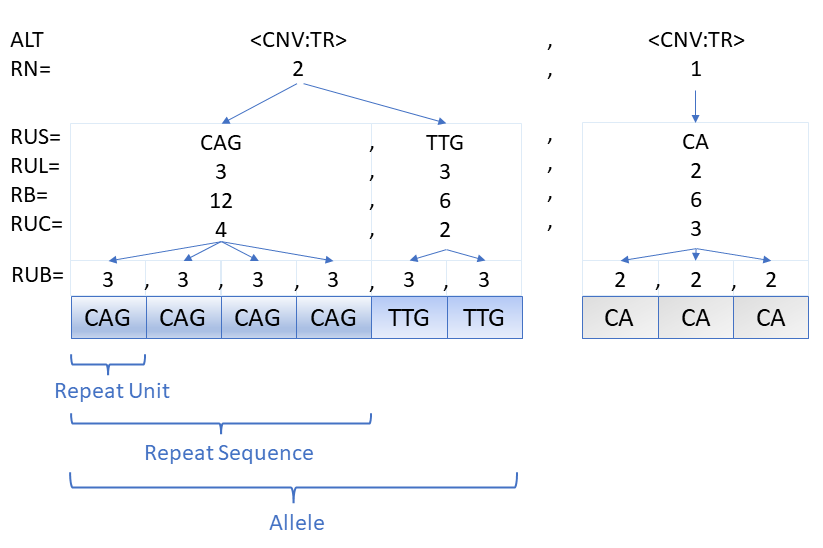
\includegraphics[width=4in,height=2.58in]{img/tandem_repeat_notation.png}
	\caption{$<$CNV:TR$>$ Tandem Repeats}
\end{figure}


A tandem repeat allele can be described by both a $<$CNV:TR$>$ 'summary' record as well as non-symbolic records.
When possible, these records should be phased with their corresponding $<$CNV:TR$>$ record as outlined in the following example.
In the following example, the reference genome contains a $(CAG)_{10}$ repeat at positions 101 to 130 inclusive, the first allele expands this to $(CAG)_{30}$ and the second allele is missing a $G$ from the 6th repeat unit $(CAG)_{5}(CA)_{1}(CAG)_{4}$:

\pagebreak
\footnotesize
\begin{landscape}
\begin{verbatim}
##fileformat=VCFv4.5
##INFO=<ID=SVLEN,Number=A,Type=Integer,Description="Length of structural variant">
##INFO=<ID=CN,Number=A,Type=Float,Description="Copy number of allele">
##INFO=<ID=RN,Number=A,Type=Integer,Description="Total number of repeat sequences in this allele">
##INFO=<ID=RUS,Number=.,Type=String,Description="Repeat unit sequence of the corresponding repeat sequence">
##INFO=<ID=RUL,Number=.,Type=Integer,Description="Repeat unit length of the corresponding repeat sequence">
##INFO=<ID=RUC,Number=.,Type=Float,Description="Repeat unit count of corresponding repeat sequence">
##INFO=<ID=RB,Number=.,Type=Integer,Description="Total number of bases in the corresponding repeat sequence">
##INFO=<ID=CIRUC,Number=.,Type=Float,Description="Confidence interval around RUC">
##INFO=<ID=CIRB,Number=.,Type=Integer,Description="Confidence interval around RB">
##INFO=<ID=RUB,Number=.,Type=Integer,Description="Number of bases in each individual repeat unit">
##FORMAT=<ID=GT,Number=1,Type=String,Description="Genotype">
##FORMAT=<ID=PS,Number=1,Type=Integer,Description="Phase set">
##FORMAT=<ID=CN,Number=1,Type=Float,Description="Copy number">
##ALT=<ID=CNV:TR,Description="Tandem repeat determined based on DNA abundance">
#CHROM POS ID REF ALT QUAL FILTER INFO FORMAT sample
chr1 100 cnv_notation T <CNV:TR>,<CNV:TR> . . SVLEN=30,30;CN=3,0.9666;RUS=CAG,CAG,CA,CAG;RN=1,3;RB=90,15,2,12  GT:PS:CN 1|2:100:3.9666
chr1 117 precise_alt2 AG A . . GT:PS 0|1:100
chr1 130 precise_alt1 G GCAGCAGCAGCAGCAGCAGCAGCAGCAGCAGCAGCAGCAGCAGCAGCAGCAGCAGCAGCAG . . GT:PS 1|0:100
\end{verbatim}
\end{landscape}
\pagebreak
\normalsize

Note the following:
\begin{itemize}
    \item As with all symbolic structural variant alleles, the POS of the $<$CNV:TR$>$ record is the base immediately preceding the tandem repeat
    \item The SVLEN of the $<$CNV:TR$>$ is the length of the reference allele.
    It is not the length of the $<$CNV:TR$>$ allele.
    \item The SVLEN of the $<$CNV:TR$>$ allele of a novel (with respect to the reference) tandem repeat should be 1.
    \item The POS of the $<$CNV:TR$>$ allele of a novel (with respect to the reference) tandem repeat should be the base immediately preceding the inserted tandem repeat sequence.
    \item Both a $<$CNV:TR$>$ and one or more non-symbolic records encoding the tandem repeat can be present.
    \item $<$CNV:TR$>$ and the non-symbolic records encoding the tandem repeat should be phased if possible.
    \item When both $<$CNV:TR$>$ and the equivalent non-symbolic records are present, the $<$CNV:TR$>$ should approximately encode the sequence but is not required to encode the sequence exactly.
	For example, SNVs and indels may be omitted in the $<$CNV:TR$>$ record.
    \item Variant callers which do not report allele-specific tandem repeats should use a single $<$CNV:TR$>$ ALT allele and the missing genotype for the GT field (for example, $./.$ if diploid).
    \item The INFO and FORMAT CN fields should be present for $<$CNV:TR$>$ records (as they are $<$CNV$>$ records) and, when present, must correspond to the sample allelic length divided by the reference allelic length.
	Note that CN FORMAT field represents the overall copy number and the INFO CN the allele-specific copy number.
    \item When benchmarking tandem repeats, the $<$CNV:TR$>$ interval provides a region over which a set of (preferably phased) non-symbolic records can be compared against for length and sequence composition.
    \item RN encodes the number of records for each allele in the RUS, RUL, RUC, RB fields.
	Conceptually, this a mechanism to encode a list-of-list with flat list format used in VCF.
    \item STRs should use RUS, whereas VNTRs should use RUL to ensure the VCF records are not excessively large.
    \item RUL should be omitted when RUS is present (as it is redundant when RS is present).
    \item RUS or RUL must be specified for each $<$CNV:TR$>$.
    \item Support for multiple levels of repeat nesting (such as STRs within VNTRs) is limited to the RUL repeat unit length field which allows the overall length of each top-level repeat unit to be encoded.
    \item The POS and SVLEN of $<$CNV:TR$>$ records should match the STR/VNTR reference catalog sizes for catalog-based callers.
    \item Variant normalisation has limited utility in regions of low complexity as almost identical haplotypes can have very different normalised representations.
\end{itemize}

In some cases, it is desirable to report the full repeat sequence of all alleles at a given repeat locus in a single VCF records.
There are no restrictions on doing so and in the above example, instead of reporting $precise\_alt1$ and $precise\_alt2$, the variants can be represented directly in a single record with a $REF$ of:
\scriptsize
\begin{verbatim}
CAGCAGCAGCAGCAGCAGCAGCAGCAGCAG
\end{verbatim}
\normalsize
and an $ALT$ of:
\scriptsize
\begin{verbatim}
CAGCAGCAGCAGCAGCAGCAGCAGCAGCAGCAGCAGCAGCAGCAGCAGCAGCAGCAGCAGCAGCAGCAGCAGCAGCAGCAGCAGCAGCAG,CAGCAGCAGCAGCAGCACAGCAGCAGCAG
\end{verbatim}
\normalsize

When the length or number of repeat units in a repeat sequence cannot be determined precisely, CIRB and/or CIRUC can be used to define the bounds.
For example, if the total number of $CAG$ repeats at the above locus was at least 50 ($(CAG)_{50-}$) and the mostly likely number of repeats was 65, then the $<$CNV:TR$>$ could be encoded as follows:

\footnotesize
\begin{verbatim}
chr1 100 . T <CNV:TR> . . SVLEN=30;CN=6.5;RUS=CAG;RUC=65;CIRUC=-15,. GT ./.
\end{verbatim}
\normalsize

Note that:
\begin{itemize}
	\item RN was omitted as it is only required if at least one $<$CNV:TR$>$ allele has RN greater than 1.
	\item The confidence interval bounds are relative to the nominal value.
	\item A missing upper bound indicates the maximum length is not known.
\end{itemize}

Exactly representing nested repeats results in the loss of some repeat information when representing with a $<$CNV:TR$>$ record.
For repeats such as $((ACCGGC)_{4}(ACCAGT))_{3-5}$, summarising the repeat structure in a $<$CNV:TR$>$ record requires either unrolling the inner repeats, or treating each outer repeat as a separate repeat sequence (the full repeat structure can be stored in a caller-specific non-standard INFO field).
For many VNTRs, the critical information to retain is the length of each repeat unit.
This length information can be encoded in the RUB field.
For example, a 10,000bp VNTRs domain repeated 5 times, each repeat 500bp longer than the previous can be encoded as follows:

\footnotesize
\begin{verbatim}
chr1 1000000 . T <CNV:TR> . . SVLEN=20000;CN=1.25;RUL=10000;RUC=5;RUB=10000,10500,11000,11500,12000 GT ./.
\end{verbatim}
\normalsize


	
	
\pagebreak
\section{BCF specification}

VCF is very expressive, accommodates multiple samples, and is widely used in the community.
Its biggest drawback is that it is big and slow.
Files are text and therefore require a lot of space on disk.
A normal batch of a hundred exomes is a few GB, but large-scale VCFs with thousands of exome samples quickly become hundreds of GBs.
Because the file is text, it is extremely slow to parse.

Overall, the idea behind is BCF2 is simple.
BCF2 is a binary, compressed equivalent of VCF that can be indexed with tabix and can be efficiently decoded from disk or streams.
For efficiency reasons BCF2 only supports a subset of VCF, in that all info and genotype fields must have their full types specified.
That is, BCF2 requires that if e.g.\ an info field {\tt AC} is present then it must contain an equivalent VCF header line noting that {\tt AC} is an allele indexed array of type integer.

\subsection{Overall file organization}

A BCF2 file is composed of a mandatory header, followed by a series of BGZF compressed blocks of binary BCF2 records.
The BGZF blocks allow BCF2 files to be indexed with tabix.

BGZF blocks are composed of a VCF header with a few additional records and a block of records.
Following the last BGZF BCF2 record block is an empty BGZF block (a block containing zero type of data), indicating that the records are done.

A BCF2 header follows exactly the specification as VCF, with a few extensions/restrictions:
\begin{itemize}
  \item All BCF2 files must have fully specified contigs definitions.
  No record may refer to a contig not present in the header itself.

  \item All INFO and GENOTYPE fields must be fully typed in the BCF2 header to enable type-specific encoding of the fields in records.
  An error must be thrown when converting a VCF to BCF2 when an unknown or not fully specified field is encountered in the records.
\end{itemize}

\subsection{Header}

The BCF2 header contains the following items:

\vspace{0.3cm}
{\small
\begin{tabular}{|l | l | p{30em} | } \hline
\textbf{Field} & \textbf{Type} & \textbf{Notes} \\ \hline
magic          & char[3]     & The characters ``{\tt BCF}'' \\ \hline
major\_version & uint8\_t    & 2 \\ \hline
minor\_version & uint8\_t    & 2 \\ \hline
l\_text        & uint32\_t   & Length of the ``text'' field, including the terminating NUL character \\ \hline
text           & char[l\_text] & VCF format header text, NUL-terminated \\ \hline
\end{tabular}}
\vspace{0.3cm}

The ``magic'' field and version numbers can be used to quickly examine the file to determine that it's a BCF2.2 file.
The ``text'' field contains the standard VCF header lines in text format, from \verb|##fileformat|
to \verb|#CHROM ...| inclusive, terminated by a NUL character.

Because the type is encoded directly in the header, the recommended extension for BCF2 formatted files is {\sl .bcf}.
BCF2 supports encoding values in a dictionary of strings.
The string map is provided by the keyword \verb|##dictionary=S0,S1,...,SN| as a comma-separate ordered list of strings.
See the ``Dictionary of strings'' section for more details.

\subsubsection{Dictionary of strings}

Throughout the BCF file most string values are be specified by integer reference to their dictionary values.
For example, the following VCF record:
\small
\begin{verbatim}
##INFO=<ID=ASP,Number=0,Type=Flag,Description="X">
##INFO=<ID=RSPOS,Number=1,Type=Integer,Description="Y">
##INFO=<ID=dbSNPBuildID,Number=1,Type=Integer,Description="Z">
##contig=<ID=20,length=62435964,assembly=B36,md5=f126cdf8a6e0c7f379d618ff66beb2da,species="Homo sapiens">
#CHROM POS ID REF ALT QUAL FILTER INFO
20 10144 rs144773400 TA T . PASS ASP;RSPOS=10145,dbSNPBuildID=134
20 10228 rs143255646 TA T . PASS ASP;RSPOS=10229;dbSNPBuildID=134
\end{verbatim}
\normalsize
would be encoded inline in BCF2 by reference to the relative position of the header line in the header (ASP=1, RSPOS=2, dbSNPBuildID=3, and PASS implicitly encoded in the first offset PASS=0).

\small
\begin{verbatim}
##INFO=<ID=ASP,Number=0,Type=Flag,Description="X">
##INFO=<ID=RSPOS,Number=1,Type=Integer,Description="Y">
##INFO=<ID=dbSNPBuildID,Number=1,Type=Integer,Description="Z">
##contig=<ID=20,length=62435964,assembly=B36,md5=f126cdf8a6e0c7f379d618ff66beb2da,species="Homo sapiens">
#CHROM POS ID REF ALT QUAL FILTER INFO
0 10144 rs144773400 TA T . s0 s1;s2=10145;s3=134
0 10228 rs143255646 TA T . s0 s1;s2=10229;s3=134
\end{verbatim}
\normalsize

Defined this way, the dictionary of strings depends on the order and the presence of all preceding header lines.
If an existing tag needs to be removed from a BCF, also all consequent tags throughout the whole BCF would have to be recoded.
In order to avoid this costly operation, a new IDX field can be used to explicitly define the position which is dropped on BCF-to-VCF conversion.
If not present, the implicit relative position is assumed.
If the IDX field is present in one record, it must be present also in all other dictionary-defining records.
The IDX tag is not necessary in newly created BCF files, but if present, the numbering must match the implicit dictionary of tags.

Note that the dictionary encoding has the magic prefix `s' here to indicate that the field's value is actually in the dictionary entry giving by the subsequent offset.
This representation isn't actually the one used in BCF2 records but it provides a clean visual guide for the above example.
Note also how the contig has been recoded as a offset into the list of contig declarations.

Note that ``PASS'' is always implicitly encoded as the first entry in the header dictionary.
This is because VCF allows FILTER fields to be PASS without explicitly listing this in the FILTER field itself.


\subsubsection{Dictionary of contigs}

The CHROM field in BCF2 is encoded as an integer offset into the list of \verb|##contig| field headers in the VCF header.
The offsets begin, like the dictionary of strings, at 0.
So for example if in BCF2 the contig value is 10, this indicates that the actual chromosome is the 11th element in the ordered list of \verb|##contig| elements.
Here's a more concrete example:

\small
\begin{verbatim}
##contig=<ID=20,length=62435964,assembly=B36,md5=f126cdf8a6e0c7f379d618ff66beb2da,species="Homo sapiens">
##contig=<ID=21,length=46944323,assembly=B36,md5=f1b74b7f9f4cdbaeb6832ee86cb426c6,species="Homo sapiens">
##contig=<ID=22,length=49691432,assembly=B36,md5=2041e6a0c914b48dd537922cca63acb8,species="Homo sapiens">
#CHROM POS ID REF ALT QUAL FILTER INFO
20 1 . T A . PASS .
21 2 . T A . PASS .
22 3 . T A . PASS .
\end{verbatim}
\normalsize

the actual CHROM field values in the encoded BCF2 records would be 0, 1, and 2 corresponding to the first (offset 0) \verb|##contig| element, etc.

\subsection{BCF2 records}

In BCF2, the original VCF records are converted to binary and encoded as BGZF blocks.
Each record is conceptually two parts.
First is the site information (chr, pos, INFO field).
Immediately after the sites data is the genotype data for every sample in the BCF2 file.
The genotype data may be omitted entirely from the record if there is no genotype data in the VCF file.
Compression of a BCF file is recommended but not required.

\subsubsection{Site encoding}
\label{BcfSiteEncoding}

{\small
\begin{tabular}{|l | l | p{30em} | } \hline
\textbf{Field} &	\textbf{Type} &	\textbf{Notes} \\ \hline
l\_shared & uint32\_t & Data length from CHROM to the end of INFO \\ \hline
l\_indiv  & uint32\_t & Data length of FORMAT and individual genotype fields \\ \hline
CHROM     & int32\_t  & Given as an offset into the mandatory contig dictionary \\ \hline
POS       & int32\_t  & 0-based leftmost coordinate \\ \hline
rlen      & int32\_t  & Length of the record as projected onto the reference sequence.
                        Must be the maximum of the length of the REF allele and the lengths
                        inferred from the SVLEN/LEN of any symbolic alleles \\ \hline
QUAL      & float     & Variant quality; 0x7F800001 for a missing value \\ \hline
n\_info   & uint16\_t & The number of INFO fields in this record \\ \hline
n\_allele & uint16\_t & The number of REF+ALT alleles in this record \\ \hline
n\_sample & uint24\_t & The number of samples in this record, stored as a \textbf{three} byte little-endian value.
                        Note that n\_sample must be equal to the number of samples in the header \\ \hline
n\_fmt    & uint8\_t  & The number of FORMAT keys.  See \ref{GenotypeEncoding} \\ \hline
ID       & typed string & Variant identifier; 0x07 for a missing value \\ \hline
REF+ALT  & list of n\_allele typed strings & the first allele is REF (mandatory) followed by n\_alleles - 1 ALT
                                             alleles, all encoded as typed strings \\ \hline
FILTER   & Typed vector of integers & a vector of integer offsets into dictionary, one for each FILTER field value.
                                      ``.'' is encoded as MISSING \\ \hline
INFO     & field key/value pairs & n\_info pairs of typed vectors.
                                   The first value must be a typed atomic integer giving the offset of the INFO field
                                   key into the dictionary.
                                   The second value is a typed vector giving the value of the field \\ \hline
Genotype values & see below & see below \\ \hline
\end{tabular}}

\subsubsection{Genotype encoding}
\label{GenotypeEncoding}

Genotype fields are encoded not by sample as in VCF but rather by field, with a vector of values for each sample following each field.
In BCF2, the following VCF line:

\vspace{0.3cm}
\begin{tabular}{l l l l}
FORMAT & NA00001 & NA00002 & NA00003 \\
GT:GQ:DP & 0/0:48:1 & 0/1:9:8 & 1/1:43:5 \\
\end{tabular}
\vspace{0.3cm}

would encoded as the equivalent of:

\vspace{0.3cm}
\begin{tabular}{l l l l}
GT=0/0,0/1,1/1 & GQ=48,9,43 & DP=1,8,5
\end{tabular}
\vspace{0.3cm}

Suppose there are i genotype fields in a specific record.
Each i is encoded by a triplet:

BCF2 site information encoding

\vspace{0.3cm}
\small
\begin{tabular}{ | p{2cm} | p{2.5cm} | p{9.5cm} | } \hline
Field & Type & Notes \\ \hline
fmt\_key & typed int & Format key as an offset into the dictionary \\ \hline
fmt\_type & uint8\_t+ & Typing byte of each individual value, possibly followed by a typed int for the vector length.  
In effect this is the same as the typing value for a single vector, but for genotype values it appears only once before the array of genotype field values \\ \hline
\makecell[tl]{fmt\_values \\ (by fmt type)} & Array of values & The information of each individual is concatenated in the vector.  Every value is of the same fmt type.
Variable-length vectors are padded with END\_OF\_VECTOR values; a string is stored as a vector of char \\  \hline
\end{tabular}
\normalsize
\vspace{0.3cm}

The value is always implicitly a vector of N values, where N is the number of samples.
The type byte of the value field indicates the type of each value of the N length vector.
For atomic values this is straightforward (size = 1).
But if the type field indicates that the values are themselves vectors (as often occurs, such as with the PL field) then each of the N values in the outer vector is itself a vector of values.
This encoding is efficient when every value in the genotype field vector has the same length and type.

It is recommended to respect the ordering as specified in the input VCF/BCF2 file, but parsers should not rely on a specific ordering.

If there are no sample records (genotype data) in this VCF/BCF2 file, the size of the genotypes block will be 0.


\subsubsection{Type encoding}
\label{BcfTypeEncoding}

In BCF2 values are all strongly typed in the file.
The type information is encoded in a prefix byte before the value, which contains information about the low-level type of the value(s) such as int32 or float, as well as the number of elements in the value.
The encoding is as follows:

\vspace{0.3cm}
\textbf{BCF2 type descriptor byte}

\vspace{0.3cm}
\begin{tabular}{|p{2cm} | p{10cm}|} \hline
Bit & Meaning \\ \hline
5,6,7,8 bits & The number of elements of the upcoming type. 
For atomic values, the size must be 1. 
If the size is set to 15, this indicates that the vector has 15 or more elements, and that the subsequent BCF2 byte stream contains a typed Integer indicating the true size of the vector. 
If the size is between 2--14, then this Integer is omitted from the stream and the upcoming stream begins immediately with the first value of the vector.
A size of 0 indicates that the value is MISSING. \\ \hline
1,2,3,4 bits & Type \\ \hline
\end{tabular}
\vspace{0.3cm}

The final four bits encodes an unsigned integer that indicates the type of the upcoming value in the data stream.

\textbf{BCF2 types}

\vspace{0.3cm}
\begin{tabular}{|l | l | l|} \hline
Lowest 4 bits & Hexadecimal encoding & Corresponding atomic type \\ \hline
0 & 0x00 & A MISSING value without an explicit type provided \\ \hline
1 & 0x?1 & Integer [8 bit] \\ \hline
2 & 0x?2 & Integer [16 bit] \\ \hline
3 & 0x?3 & Integer [32 bit] \\ \hline
5 & 0x?5 & Float [32 bit] \\ \hline
7 & 0x?7 & Character, ASCII encoded in 8 bits \\ \hline
\end{tabular}
\vspace{0.3cm}

In BCF2 strings are type=7 with an appropriate length.
Single characters are represented as strings with length=1.
Type codes 4,6,8--15 are reserved for future use.

\vspace{0.3cm}

\textbf{Integers} may be encoded as 8, 16, or 32 bit values, in little-endian order.
It is up to the encoder to determine the appropriate ranged value to use when writing the BCF2 file.
For integer types, the values 0x80, 0x8000, 0x80000000 are interpreted as missing values and 0x81, 0x8001, 0x80000001 as END\_OF\_VECTOR indicators (for 8, 16, and 32 bit values, respectively).
Note that the END\_OF\_VECTOR byte is not part of the vector itself and only END\_OF\_VECTOR bytes can follow.
In total, eight values are reserved for future use: 0x80--0x87, 0x8000--0x8007, 0x80000000--0x80000007.

\vspace{0.3cm}
\textbf{Floats} are encoded as single-precision (32 bit) in the basic format defined by the IEEE-754-1985 standard.
This is the standard representation for floating point numbers on modern computers, with direct support in programming languages like C and Java (see Java's Double class for example).
BCF2 supports the full range of values from -Infinity to +Infinity, including NaN.
BCF2 needs to represent missing values for single precision floating point numbers.
This is accomplished by writing the NaN value as the quiet NaN (qNaN), while the MISSING value is encoded as a signaling NaN.
From the NaN wikipedia entry, we have:

\begin{quote}
For example, a bit-wise example of a IEEE floating-point standard single precision (32-bit) NaN would be: s111 1111 1axx xxxx xxxx xxxx xxxx xxxx where s is the sign (most often ignored in applications), a determines the type of NaN, and x is an extra payload (most often ignored in applications).
If a = 1, it is a quiet NaN; if a is zero and the payload is nonzero, then it is a signaling NaN.
\end{quote}

\noindent A good way to understand these values is to play around with the IEEE encoder website.

\vspace{0.3cm}
\noindent Similarly to integers, the float value of 0x7F800001 is interpreted as a MISSING value and 0x7F800002 as the END\_OF\_VECTOR indicator. 
Note that the END\_OF\_VECTOR byte is not part of the vector itself and only END\_OF\_VECTOR bytes can follow.
In total, eight values are reserved for future use:


\vspace{0.1cm}
\begin{tabular}{| l | c | l |} \hline
\textbf{Value}   & \textbf{32-bit precision} & \textbf{Hexadecimal representation} \\ \hline
NaN	    & 0b0111 1111 1100 0000 0000 0000 0000 0000 & 0x7FC00000 \\ \hline
MISSING & 0b0111 1111 1000 0000 0000 0000 0000 0001 & 0x7F800001 \\ \hline
END\_OF\_VECTOR & 0b0111 1111 1000 0000 0000 0000 0000 0010 & 0x7F800002 \\ \hline
reserved & 0b0111 1111 1000 0000 0000 0000 0000 0011 & 0x7F800003 \\ \hline
$\ldots$ & $\ldots$ & $\ldots$ \\ \hline
reserved & 0b0111 1111 1000 0000 0000 0000 0000 0111 & 0x7F800007 \\ \hline
\end{tabular}

\vspace{0.3cm}
\textbf{Character} values are not explicitly typed in BCF2.
Instead, VCF Character values must be encoded by a single character string. See also \ref{character-encoding}.

\vspace{0.3cm}
\textbf{Flags} values --- which can only appear in INFO fields --- in BCF2 should be encoded by any non-reserved value.
The recommended best practice is to encode the value as an 1-element INT8 (type 0x11) with value of 1 to indicate present.
Because FLAG values can only be encoded in INFO fields, BCF2 provides no mechanism to encode FLAG values in genotypes, but could be easily extended to do so if allowed in a future VCF version.

\vspace{0.3cm}
\textbf{String} values have two basic encodings.
For INFO, FORMAT, and FILTER keys these are encoded by integer offsets into the header dictionary.
For string values, such as found in the ID, REF, ALT, INFO, and FORMAT fields, strings are encoded as typed array of ASCII encoded bytes.
The array isn't terminated by a NUL byte.
The length of the string is given by the length of the type descriptor.

Suppose you want to encode the string ``{\tt ACAC}''.
First, we need the type descriptor byte, which is the string type 0x07 or'd with inline size (4) yielding the type byte of 0x40 $|$ 0x07 = 0x47.
Immediately following the type byte is the four byte ASCII encoding of ``{\tt ACAC}'': 0x41 0x43 0x41 0x43.
So the final encoding is:

\vspace{0.1cm}
\begin{tabular}{| l | l |} \hline
0x47 0x41 0x43 0x41 0x43 & String type with inline size of 4 followed by ACAC in ASCII \\ \hline
\end{tabular}
\vspace{0.3cm}

Suppose you want to encode the string ``{\tt VariantCallFormatSampleText}'', a string of size 27.
First, we need the type descriptor byte, which is the string type 0x07.
Because the size exceeds the inline size limit ($27 \geq 15$) we set the size to overflow, yielding the type byte of 0xF0 $|$ 0x07 = 0xF7.
Immediately following the type byte is the typed size of 27, which we encode by the atomic INT8 value: 0x11 followed by the actual size 0x1B.
Finally comes the actual bytes of the string: 0x56 0x61 0x72 0x69 0x61 0x6E 0x74 0x43 0x61 0x6C 0x6C 0x46 0x6F 0x72 0x6D 0x61 0x74 0x53 0x61 0x6D 0x70 0x6C 0x65 0x54 0x65 0x78 0x74.
So the final encoding is:

\vspace{0.3cm}
\begin{tabular}{ | p{9cm} | p{6cm} | } \hline
0xF7 & string with overflow size \\ \hline
0x11 0x1B & overflow size encoded as INT8 with value 27 \\ \hline
0x56 0x61 0x72 0x69 0x61 0x6E 0x74 0x43 0x61 0x6C 0x6C 0x46 0x6F 0x72 0x6D 0x61 0x74 0x53 0x61 0x6D 0x70 0x6C 0x65 0x54 0x65 0x78 0x74 & message in ASCII \\ \hline
\end{tabular}
\vspace{0.3cm}

Suppose you want to encode the missing value `.'.
This is simply a string of size 0 = 0x07.

\vspace{0.3cm}
In VCF there are sometimes fields of type list of strings, such as a number field of unbounded size encoding the amino acid changes due to a mutation.
Since BCF2 doesn't directly support vectors of strings (a vector of character is already a string) we collapse the list of strings into a single comma-separated string, encode it as a regular BCF2 vector of characters, and on reading explode it back into the list of strings.
This works because strings in VCF cannot contain `{\tt ,}' (it's a field separator) and so we can safely use `{\tt ,}' to separate the individual strings.

% String vectors in BCF do not need to start with comma, as the number of
% values is indicated already in the definition of the tag in the header.
%
% For efficiency
% reasons we put a comma at the start of the collapsed string, so that just the
% first character can be examined to determine if the string is collapsed.
%END\_OF\_VECTOR
% To be concrete, suppose we have a info field around X=[A,B,C,D].  This is
% encoded in BCF2 as a single string ``,A,B,C,D'' of size 8, so it would have
% type byte 0x87 followed by the ASCII encoding 0x2C 0x41 0x2C 0x42 0x2C 0x43
% 0x2C 0x44.

\vspace{0.3cm}

\textbf{Vectors} --- The BCF2 type byte may indicate that the upcoming data stream contains not a single value but a fixed length vector of values.
The vector values occur in order (1st, 2nd, 3rd, etc) encoded as expected for the type declared in the vector's type byte.
For example, a vector of 3 16-bit integers would be laid out as first the vector type byte, followed immediately by 3 2-byte values for each integer, including a total of 7 bytes.

Missing values in vectors are handled slightly differently from atomic values.
There are two possibilities for missing values:

One (or more) of the values in the vector may be missing, but others in the vector are not.
Here each value should be represented in the vector, and each corresponding BCF2 vector value either set to its present value or the type equivalent MISSING value.
Alternatively the entire vector of values may be missing.
In this case the correct encoding is as a type byte with size 0 and the appropriate type MISSING.
Suppose we are encoding the record ``AC=[1,2,3]'' from the INFO field.
The AC key is encoded in the standard way.
This would be immediately followed by a typed 8-bit integer vector of size 3, which is encoded by the type descriptor 0x31.
The type descriptor is immediately followed by the three 8-bit integer values: 0x01 0x02 0x03, for a grand total of 4 bytes: 0x31010203.

Suppose we are at a site with many alternative alleles so AC=[1,2,3,4,5,6,7,8,9,10,11,12,13,14,15,16].
Since there are 16 values, we have to use the long vector encoding.
The type of this field is 8 bit integer with the size set to 15 to indicate that the size is the next stream value, so this has type of 0xF1.
The next value in the stream is the size, as a typed 8-bit atomic integer: 0x11 with value 16 0x10.
Each integer AC value is represented by it's value as a 8 bit integer.
The grand total representation here is:

\vspace{0.3cm}
\begin{tabular}{|p{9cm} | p{6cm}|} \hline
0xF1 0x01 0x10 & 8 bit integer vector with overflow size \\ \hline
0x01 0x02 0x03 0x04 0x05 0x06 0x07 0x08 0x09 0x0A 0x0B 0x0C 0x0D 0x0E 0x0F 0x10 & 1--16 as hexadecimal 8 bit integers \\ \hline
\end{tabular}
\vspace{0.3cm}

Suppose this INFO field contains the ``AC=.'', indicating that the AC field is missing from a record with two alt alleles.
The correct representation is as the typed pair of AC followed by a MISSING vector of type 8-bit integer: 0x01.

\vspace{0.3cm}
\textbf{Vectors of mixed length} --- In some cases genotype fields may be vectors whose length differs among samples.  
For example, some CNV call sets encode different numbers of genotype likelihoods for each sample, given the large number of potential copy number states, rather padding all samples to have the same number of fields.  
For example, one sample could have CN0:0,CN1:10 and another CN0:0,CN1:10,CN2:10.  
In the situation when a genotype field contain vector values of different lengths, these are represented in BCF2 by a vector of the maximum length per sample, with all values in the each vector aligned to the left, and END\_OF\_VECTOR values assigned to all values not present in the original vector.  
The BCF2 encoder / decoder must automatically add and remove these END\_OF\_VECTOR values from the vectors. Note that the use of END\_OF\_VECTOR means that it is legal to encode a vector VCF field with MISSING values.

For example, suppose I have two samples, each with a FORMAT field X.  
Sample A has values [1], while sample B has [2,3].  
In BCF2 this would be encoded as [1, END\_OF\_VECTOR] and [2, 3]. 
Diving into the complete details, suppose X is at offset 3 in the dictionary, which is encoded by the typed INT8 descriptor 0x11 followed by the value 0x03. 
Next we have the type of the each format field, which here is a 2 element INT8 vector: 0x21.  
Next we have the encoding for each sample, A = 0x01 0x81 followed by B = 0x02 0x03.  
All together we have:

\vspace{0.3cm}
\begin{tabular}{|p{2cm} | l |} \hline
0x11 0x03 & X dictionary offset \\ \hline
0x21 & each value is a 2 element INT8 value \\ \hline
0x01 0x81 & A is [1, END\_OF\_VECTOR] \\ \hline
0x02 0x03 & B is [2, 3] \\ \hline
\end{tabular}
\vspace{0.3cm}


\vspace{0.3cm}
A \textbf{Genotype (GT) field} is encoded in a typed integer vector (can be 8, 16, or even 32 bit if necessary) with the number of elements equal to the maximum ploidy among all samples at a site.
For one individual, each integer in the vector is organized as $(allele+1) << 1 \mid phased$ where allele is set to $-1$ if the allele in GT is a dot `.' (thus the higher bits are all 0).
The vector is padded with the END\_OF\_VECTOR values if the GT having fewer ploidy.
We note specifically that except for the END\_OF\_VECTOR byte, no other negative values are allowed in the GT array.
When processing VCF version 4.3 or earlier files, the phasing of the first allele should be treated as missing and inferred from the remaining alleles.

Examples:

\vspace{0.3cm}
\small
\begin{tabular}{|p{2.5cm} | p{10cm} | p{3cm}|} \hline
0/1 & in standard format $(0 + 1) << 1 \mid 0$ followed by $(1 + 1) << 1 \mid 0$ & 0x02 04 \\ \hline
0/1, 1/1, and 0/0 & three samples encoded consecutively & 0x02 04 04 04 02 02 \\ \hline
$0\mid1$ & $(1 + 1) << 1 \mid 1$ = 0x05 preceded by the phased first byte value 0x03 & 0x03 05 \\ \hline
./. & where both alleles are missing & 0x00 00 \\ \hline
0 & as an implicitly phased haploid it is represented by a single byte & 0x03 \\ \hline
1 & as an implicitly phased haploid it is represented by a single byte & 0x05 \\ \hline
0/1/2 & is tetraploid, with alleles & 0x02 04 06 \\ \hline
$0/1\mid2$ & is tetraploid with a single phased allele & 0x02 04 07 \\ \hline
0 and 0/1 & pad out the final allele for the haploid individual & 0x02 81 02 04\\ \hline
\end{tabular}
\normalsize

\vspace{0.3cm}
The final example is something seen on chrX when we have a haploid male and a diploid female.
The male genotype vector is terminated prematurely by the END\_OF\_VECTOR value.
\vspace{0.3cm}


\subsection{Encoding a VCF record example}

Let's encode a realistic (but made-up) VCF record.
This is a A/C SNP in HM3 (not really) called in~3 samples.
In this section we'll build up the BCF2 encoding for this record.
\scriptsize
\begin{verbatim}
#CHROM POS ID REF ALT QUAL FILTER INFO FORMAT NA00001 NA00002 NA00003
chr1 101 rs123 A C 30.1 PASS HM3;AC=3;AN=6;AA=C GT:GQ:DP:AD:PL 0/0:10:32:32,0:0,10,100 0/1:10:48:32,16:10,0,100 1/1:10:64:0,64:100,10,0
\end{verbatim}
\normalsize

\subsubsection{Encoding CHROM and POS}

First, let's assume that {\tt chr1} is the second chromosome to appear in the contig list---right after {\tt chrM} ({\tt MT}).
So its offset is 1.
The {\tt POS} BCF2 field value is~101 (obviously).
Because these are both typed values in the BCF2 record, we encode both in their most compact 8-bit value form.
The type byte for an atomic 8-bit integer is 0x11.
The value for the contig offset is 1 = 0x01.
The value 101 is encoded as the single byte 0x65.
So in total these are represented as:

\vspace{0.3cm}
\begin{tabular}{|l | l|} \hline
0x01000000 & CHROM offset is at 1 in 32 bit little endian \\ \hline
0x64000000 & POS in 0 base 32 bit little endian \\ \hline
0x01000000 & rlen = 1 (it's just a SNP) \\ \hline
\end{tabular}

\subsubsection{Encoding QUAL}

The QUAL field value is 30.1, which we encode as an untyped single precision 32-bit float:

\vspace{0.3cm}
\begin{tabular}{|l| l|} \hline
0x41 0xF0 0xCC 0xCD & QUAL = 30.1 as 32-bit float \\ \hline
\end{tabular}

\subsubsection{Encoding ID}

This ID value is a 5-element string, so is encoded as type descriptor 0x57 followed by the five bytes for the string of {\tt 0x72 0x73 0x31 0x32 0x33}.
The full encoding is:

\vspace{0.3cm}
\begin{tabular}{|l| l|} \hline
0x57 0x72 0x73 0x31 0x32 0x33 & ID = rs123 \\ \hline
\end{tabular}

\subsubsection{Encoding REF/ALT fields}

We encode each of REF and ALT as typed strings, first REF followed immediately by ALT.
Each is a 1 element string (0x17), which would then be followed by the single bytes for the bases of 0x43 and 0x41:

\vspace{0.3cm}
\begin{tabular}{|l| l|} \hline
0x17 0x41 & REF A \\ \hline
0x17 0x43 & ALT C \\ \hline
\end{tabular}

\vspace{0.3cm}
Just for discussion, suppose instead that ALT was ALT=C,T.
The only thing that could change is that there would be another typed string following immediately after C encoding 0x17 (1 element string) with the value of 0x54.

\subsubsection{Encoding FILTER}

``PASS'' is implicitly encoded as the first entry in the header dictionary (see dictionary of strings).
Here we encode the PASS FILTER field as a vector of size 1 of type 8-bit, which has type byte is 0x11.
The value is the offset 0:

\vspace{0.3cm}
\begin{tabular}{|l| l|} \hline
0x11 0x00 & FILTER field PASS \\ \hline
\end{tabular}

\subsubsection{Encoding the INFO fields}

HM3;AC=3;AN=6;AA=C
Let's assume that the header dictionary elements for HM3, AC, AN, and AA are at 80, 81, 82, and 83 respectively.
All of these can be encoded by 1-element INT8 values (0x11), with associated hex values of 0x50, 0x51, 0x52, and 0x53 respectively.

First is HM3.
The entry begins with the key: 0x11 0x50.
The HM3 field is a flag with no associated value and therefore the rest of the entry is the special case of a missing value without an explicit type provided.
Altogether we have:

\vspace{0.3cm}
\begin{tabular}{|l| l|} \hline
0x11 0x50 0x00 & HM3 flag is present \\ \hline
\end{tabular}
\vspace{0.3cm}

Now let's encode the two atomic 8-bit integer fields AC and AN:

\vspace{0.3cm}
\begin{tabular}{|l| l|} \hline
0x11 0x51 & AC key \\ \hline
0x11 0x03 & with value of 3 \\ \hline
0x11 0x52 & AN key \\ \hline
0x11 0x06 & with value of 6 \\ \hline
\end{tabular}
\vspace{0.3cm}

The ancestral allele (AA) tell us that among other primates the original allele is C, a Character here.
Because we represent Characters as single element strings in BCF2 (0x17) with value 0x43 (C).
So the entire key/value pair is:

\vspace{0.3cm}
\begin{tabular}{|l |l|} \hline
0x11 0x53 & AA key \\ \hline
0x17 0x43 & with value of C \\ \hline
\end{tabular}

\subsubsection{Encoding Genotypes}

Continuing with our example:

\vspace{0.3cm}
\begin{tabular}{l l l l}
FORMAT & NA00001 & NA00002 & NA00003 \\
GT:GQ:DP:AD:PL & 0/0:10:32:32,0:0,10,100 & 0/1:10:48:32,16:10,0,100 & 1/1:10:64:0,64:100,10,0 \\
\end{tabular}
\vspace{0.3cm}

Here we have the specially encoded GT field.
We have two integer fields GQ and DP.
We have the AD field, which is a vector of 2 values per sample.
And finally we have the PL field which is 3 values per sample.
Let's say that the FORMAT keys for GT, GQ, DP, AD, and PL are at offsets 1, 2, 3, and 4, 5, respectively.
Now let's encode each of the genotype fields in order of the VCF record (GT, GQ, DP, AD, and then PL):

GT triplet begins with the key: 0x1101.
Next is the type of the field, which will be a 2-element (diploid) INT8 type: 0x21.
This is followed by 3 2-byte arrays of values 0x0202 0x0204 0x0404 (see genotype encoding example for details).
The final encoding is 0x1101 0x21 0x020202040404

GQ triplet begins with the key 0x1102.
Because these values are small, we encode them as 8 bit atomic integers with type code 0x11.
As each value is the same (10 = 0x0A) the GQ field is encoded as 0x1102 0x11 0x0A0A0A

DP almost identical to GQ.
First is the 0x1103 key, followed by 3 8-bit atomic integers encoded as 0x11 (the type) 0x20 (DP=32), 0x30 (DP=48) and 0x40 (DP=64).
So we have: 0x1103 0x11203040

AD is more complex.
The key is simple, just like the others, with 0x1104.
Because the AD field is a vector of 2 values for each genotype, the value of key/value pair a vector type.
Because the integer values in each AD field of each sample are small they are encoded by 8 bit values.
So the value type is = 0x21.
For sample one there are two values: 32,0 which are 0x30 and 0x00.
Samples two and three are 0x30 0x20 and 0x00 0x40 respectively.
So ultimately this field is encoded as 0x1104 0x21 0x300030200040

PL is just like AD but with three values per sample.
The key is 0x1105.
Because the PL field is a vector of 3 values for each genotype, the value of key/value pair a vector type, and because the size is 3 it's encoded in the size field of the type.
Again, because the integer values in each PL field of each sample are small they are encoded by 8 bit values.
So the value type 0x31.
For sample one there are three values: 0, 10, and 100 which are 0x00, 0x0A, and 0x64.
Samples two and three have the same values but in a slightly different order.
So ultimately the PL field is encoded as 0x1105 0x31 0x000A64 0x0A0064 0x640A00

So the genotype block contains:

\vspace{0.3cm}
\begin{tabular}{|l| l|} \hline
0x1101 0x21 0x020202040404 & GT \\ \hline
0x1102 0x11 0x0A0A0A & GQ \\ \hline
0x1103 0x11 0x203040 & DP \\ \hline
0x1104 0x21 0x300030200040 & AD \\ \hline
0x1105 0x31 0x000A640A0064640A00 & PL \\ \hline
\end{tabular}
\vspace{0.3cm}

\textbf{Putting it all together}

We need to determine a few values before writing out the final block:

l\_shared = 51 (Data length from CHROM to the end of INFO)

l\_indiv = 42 (Data length of FORMAT and individual genotype fields)

n\_info = 4 (Number of INFO fields)

n\_allele = 2 (Number of alleles, including REF)

n\_sample = 3 (Number of samples)

n\_fmt = 5 (Number of FORMAT keys)

\vspace{0.3cm}
\begin{tabular}{|l| l|} \hline
0x33000000 & l\_shared as 32-bit little endian hex \\ \hline
0x2A000000 & l\_indiv as 32-bit little endian hex \\ \hline
0x01000000 & CHROM offset is at 1 in 32 bit little endian \\ \hline
0x64000000 & POS in 0-based 32-bit little endian \\ \hline
0x01000000 & rlen = 1 (it's just a SNP) \\ \hline
0x41 0xF0 0xCC 0xCD & QUAL = 30.1 as 32-bit float \\ \hline
0x0400     & n\_info as 16-bit little-endian \\ \hline
0x0200     & n\_allele as 16-bit little-endian \\ \hline
0x030000   & n\_sample as 24-bit little-endian \\ \hline
0x05       & n\_fmt \\ \hline
0x57 0x72 0x73 0x31 0x32 0x33 & ID = rs123 \\ \hline
0x17 0x41 & REF A \\ \hline
0x17 0x43 & ALT C \\ \hline
0x11 0x00 & FILTER field PASS \\ \hline
0x11 0x50 0x00 & HM3 flag is present \\ \hline
0x11 0x51 & AC key \\ \hline
0x11 0x03 & with value of 3 \\ \hline
0x11 0x52 & AN key \\ \hline
0x11 0x06 & with value of 6 \\ \hline
0x11 0x53 & AA key \\ \hline
0x17 0x43 & with value of C \\ \hline
0x1101 0x21 0x020202040404 & GT \\ \hline
0x1102 0x11 0x0A0A0A & GQ \\ \hline
0x1103 0x11 0x203040 & DP \\ \hline
0x1104 0x21 0x300030200040 & AD \\ \hline
0x1105 0x31 0x000A640A0064640A00 & PL \\ \hline
\end{tabular}
\vspace{0.3cm}

That's quite a lot of information encoded in only 96 bytes!

\subsection{BCF2 block gzip and indexing}

These raw binary records may be subsequently encoded into BGZF blocks following the BGZF compression format, section 3 of the SAM format specification.
BCF2 records can be raw, though, in cases where the decoding/encoding costs of bgzipping the data make it reasonable to process the data uncompressed, such as streaming BCF2s through pipes with samtools and bcftools.
Here the files should be still compressed with BGZF but with compression 0.
Implementations should perform BGZF encoding and must support the reading of both raw and BGZF encoded BCF2 files.

BCF2 files are expected to be indexed through the same index scheme, section~4 as BAM files and other block-compressed files with BGZF.

\section{List of changes}

\subsection{Changes between VCFv4.5 and VCFv4.4}

\begin{itemize}
	\item Added base modification support (FORMAT M5mC, M5hmC, M6mA, etc.).
	\item Reserved all FORMAT keys of the form $M[0-9]+$ as base modification fields.
	\item Added Number=P support for fields with cardinality matching sample ploidy/local copy number.
	\item Added local allele support (Number=LA, LG, LR; FORMAT LAA, LAD, LADF, LADR, LEC, LGL, LGP, LPL, LPP) to reduce the size of multi-sample VCFs and enable lossless merging.
	\item Deprecated INFO END. It is now a computed field written only for backwards compatibility with older versions of VCF.
	\item Updated BCF rlen field to reflect INFO END being a computed value.
	\item Added FORMAT LEN to support sample-specific $<$*$>$ alleles.
	\item Clarified that the header line is indeed mandatory
	\item Clarified that $<$NON\_REF$>$ should be treated as an alias of $<$*$>$
\end{itemize}

\subsection{VCFv4.4 Errata}

\begin{itemize}
	\item Type=P added to FORMAT field type list (used by PSL/PSO fields)
\end{itemize}

\subsection{Changes between VCFv4.4 and VCFv4.3}

\begin{itemize}
\item Added tandem repeat support ($<$CNV:TR$>$, RN, RUS, RUL, RB, CIRB, RUC, CIRUC, RUB)
\item Redefined INFO CN as allele-specific copy number and FORMAT CN as total copy number.
\item Redefined INFO and FORMAT CN to support non-integer copy numbers.
\item Added support for phasing and derivative chromosome reconstruction in the presence of SVs (PSL, PSO, PSQ)
\item Added SVCLAIM to disambiguate copy number based $<$DEL$>$ and $<$DUP$>$ variants from breakpoint based ones.
\item Conceptually separated variant detection and interpretation.
\item Added EVENTTYPE/EVENT to enable the multiple records encoding complex genomic rearrangements to be grouped together.
\item Added polyploid partial phasing support (e.g. GT $|0|0/1/2$). GT now defined as a prefix notation with the first phasing indicator optional.
\item Redefined $Number=$ for SVLEN, CIPOS, CIEND, HOMLEN, HOMSEQ, BKPTID, MEINFO, METRANS, DGVID, DBVARID, DBRIPID, MATEID, PARID, EVENT, CN, CICN to support multiple symbolic alleles.
\item Redefined END as the end position of the longest ALT allele. Note that END remains $Number=1$.
\item Redefined SVLEN to always be positive and be meaningful for INV variants.
\item Redefined SVLEN, END and BCF rlen to support both $<*>$ and symbolic structural variant alleles in the same record.
\item Number, Type and Description required only for INFO meta-information lines
\item Clarified CIPOS should be used to define micro-homology bounds
\item Clarified INFO lines field ordering
\item Clarified that symbolic and breakpoint notation ALT alleles are case sensitive.
\item Deprecated SVTYPE
\item Removed DPADJ, CNADJ, CICNADJ
\item Disallowed BND ALT records (these should use breakpoint notation anyway)
\item Removed definition of DP from Section 3 as it was already defined in Section 1.6.1.8.
\item Deprecated bundles in favour of PSL-based phasing.
\item Updated SV examples.
\item BCF parsers should perform BGZF encoding and must support both raw and BGZF encoded files.
\end{itemize}

\subsection{Changes to VCFv4.3}

\begin{itemize}
\item More strict language: ``should'' replaced with ``must'' where appropriate
\item Tables with Type and Number definitions for INFO and FORMAT reserved keys

\item
The set of characters allowed in VCF contig names is now the same as that allowed in SAM reference sequence names, which was restricted in January 2019.
The characters `{\tt\verb|\|\,,\,"`'\,()\,\verb|{}|}' are now invalid in VCF contig names, while `{\tt *}' is now valid when not the first character.
(The characters `{\tt []\,<>}' and initial~`{\tt *}'/`{\tt =}' were already invalid and remain so.)

The VCF specification previously disallowed colons (`{\tt :}') in contig names to avoid confusion when parsing breakends, but this was unnecessary.
Even with contig names containing colons, the breakend mate position notation can be unambiguously parsed because the ``{\tt :}\emph{pos}'' part is \textbf{always} present.
\item Added PP tag which is the phred-scaled analogue to GP
\end{itemize}

\subsection{Changes between VCFv4.2 and VCFv4.3}

\begin{itemize}
\item VCF compliant implementations must support both LF and CR+LF newline conventions
\item INFO and FORMAT tag names must match the regular expression \texttt{\^{}[A-Za-z\_][0-9A-Za-z\_.]*\$}
\item Spaces are allowed in INFO field values
\item Characters with special meaning (such as `;' in INFO, `:' in FORMAT, and `\%' in both) can be encoded using percent encoding (see Section~\ref{character-encoding})
\item The character encoding of VCF files is UTF-8.
\item The SAMPLE field can contain optional DOI URL for the source data file
\item Introduced \#\#META header lines for defining phenotype metadata
\item New reserved tag ``CNP'' analogous to ``GP'' was added. Both CNP and GP use 0 to 1 encoding, which is a change from previous phred-scaled GP.
\item In order for VCF and BCF to have the same expressive power, we state explicitly that Integers and Floats are 32-bit numbers.
Integers are signed.
\item We state explicitly that zero length strings are not allowed, this includes the CHROM and ID column, INFO IDs, FILTER IDs and FORMAT IDs.
Meta-information lines can be in any order, with the exception of \#\#fileformat which must come first. 
\item All header  lines of the form \#\#key=$<$ID=xxx,...$>$ must have an ID value that is unique for a given value of ``key''.
All header lines whose value starts with ``$<$'' must have an ID field.
Therefore, also \#\#PEDIGREE newly requires a unique ID.
\item We state explicitly that duplicate IDs, FILTER, INFO or FORMAT keys are not valid.
\item A section about gVCF was added, introduced the $<$*$>$ symbolic allele.
\item A section about tag naming conventions was added.
\item New reserved AD, ADF, and ADR INFO and FORMAT fields added.
\item Removed unused and ill-defined GLE FORMAT tag.
\item Chromosome names cannot use reserved symbolic alleles and contain characters used by breakpoints (Section~\ref{sec-contig-field}).
\item IUPAC ambiguity codes should be converted to a concrete base.
\item Symbolic ALTs for IUPAC codes.
\end{itemize}

\subsection{Changes between BCFv2.1 and BCFv2.2}
\begin{itemize}
\item BCF header lines can include optional IDX field
\item We introduce END\_OF\_VECTOR byte and reserve 8 values for future use
\item Clarified that except the END\_OF\_VECTOR byte, no other negative values are allowed in the GT array 
\item String vectors in BCF do not need to start with comma, as the number of values is indicated already in the definition of the tag in the header.
\item The implicit filter PASS was described inconsistently throughout BCFv2.1: It is encoded as the first entry in the dictionary, not the last.
\end{itemize}

\subsection{Changes between VCFv4.1 and VCFv4.2}
\begin{itemize}
\item In the HEADER the INFO definition allow additional field after the 4 first mandatory fields
\item INFO fields definition can use Number=R to specify one per allele including the reference.
\item Allow star allele in the ALT for describing upstream deletion
\end{itemize}

\end{document}

\title{\huge \color{red} DRAFT SPEC SUBJECT TO CHANGE \\ The Variant Call Format Specification \\ \vspace{0.5em} \large VCFv4.5 and BCFv2.2}
\date{\headdate}
\maketitle
\begin{quote}\small
The master version of this document can be found at \url{https://github.com/samtools/hts-specs}.\\
This printing is version~\commitdesc\ from that repository, last modified on the date shown above.
\end{quote}
\vspace*{1em}

\newpage
\tableofcontents
\newpage

\section{The VCF specification}
VCF is a text file format (most likely stored in a compressed manner).
It contains meta-information lines (prefixed with ``\verb|##|''), a header line (prefixed with ``\verb|#|''), and data lines each containing information about a position in the genome and genotype information on samples for each position (text fields separated by tabs).
Zero length fields are not allowed, a dot (``.'') must be used instead.
In order to ensure interoperability across platforms, VCF compliant implementations must support both LF (``\verb|\n|'') and CR+LF (``\verb|\r\n|'') newline conventions.

\subsection{An example}
\scriptsize
\begin{verbatim}
##fileformat=VCFv4.5
##fileDate=20090805
##source=myImputationProgramV3.1
##reference=file:///seq/references/1000GenomesPilot-NCBI36.fasta
##contig=<ID=20,length=62435964,assembly=B36,md5=f126cdf8a6e0c7f379d618ff66beb2da,species="Homo sapiens",taxonomy=x>
##phasing=partial
##INFO=<ID=NS,Number=1,Type=Integer,Description="Number of Samples With Data">
##INFO=<ID=DP,Number=1,Type=Integer,Description="Total Depth">
##INFO=<ID=AF,Number=A,Type=Float,Description="Allele Frequency">
##INFO=<ID=AA,Number=1,Type=String,Description="Ancestral Allele">
##INFO=<ID=DB,Number=0,Type=Flag,Description="dbSNP membership, build 129">
##INFO=<ID=H2,Number=0,Type=Flag,Description="HapMap2 membership">
##FILTER=<ID=q10,Description="Quality below 10">
##FILTER=<ID=s50,Description="Less than 50% of samples have data">
##FORMAT=<ID=GT,Number=1,Type=String,Description="Genotype">
##FORMAT=<ID=GQ,Number=1,Type=Integer,Description="Genotype Quality">
##FORMAT=<ID=DP,Number=1,Type=Integer,Description="Read Depth">
##FORMAT=<ID=HQ,Number=2,Type=Integer,Description="Haplotype Quality">
#CHROM POS     ID        REF    ALT     QUAL FILTER INFO                              FORMAT      NA00001        NA00002        NA00003
20     14370   rs6054257 G      A       29   PASS   NS=3;DP=14;AF=0.5;DB;H2           GT:GQ:DP:HQ 0|0:48:1:51,51 1|0:48:8:51,51 1/1:43:5:.,.
20     17330   .         T      A       3    q10    NS=3;DP=11;AF=0.017               GT:GQ:DP:HQ 0|0:49:3:58,50 0|1:3:5:65,3   0/0:41:3
20     1110696 rs6040355 A      G,T     67   PASS   NS=2;DP=10;AF=0.333,0.667;AA=T;DB GT:GQ:DP:HQ 1|2:21:6:23,27 2|1:2:0:18,2   2/2:35:4
20     1230237 .         T      .       47   PASS   NS=3;DP=13;AA=T                   GT:GQ:DP:HQ 0|0:54:7:56,60 0|0:48:4:51,51 0/0:61:2
20     1234567 microsat1 GTC    G,GTCT  50   PASS   NS=3;DP=9;AA=G                    GT:GQ:DP    0/1:35:4       0/2:17:2       1/1:40:3
\end{verbatim}
\normalsize
This example shows (in order): a good simple SNP, a possible SNP that has been filtered out because its quality is below 10, a site at which two alternate alleles are called, with one of them (T) being ancestral (possibly a reference sequencing error), a site that is called monomorphic reference (i.e.\ with no alternate alleles), and a microsatellite with two alternative alleles, one a deletion of 2 bases (TC), and the other an insertion of one base (T).
Genotype data are given for three samples, two of which are phased and the third unphased, with per sample genotype quality, depth and haplotype qualities (the latter only for the phased samples) given as well as the genotypes.
The microsatellite calls are unphased.

\subsection{Character encoding, non-printable characters and characters with special meaning}
\label{character-encoding}
The character encoding of VCF files is UTF-8.
UTF-8 is a multi-byte character encoding that is a strict superset of 7-bit ASCII and has the property that none of the bytes in any multi-byte characters are 7-bit ASCII bytes.
As a result, most software that processes VCF files does not have to be aware of the possible presence of multi-byte UTF-8 characters.
VCF files must not contain a byte order mark.
Note that non-printable characters U+0000--U+0008, U+000B--U+000C, U+000E--U+001F are disallowed.
Line separators must be CR+LF or LF and they are allowed only as line separators at end of line.
Some characters have a special meaning when they appear (such as field delimiters `\verb|;|' in INFO or `\verb|:|' FORMAT fields), and for any other meaning they must be represented with the capitalized percent encoding:

\begingroup\footnotesize
\begin{tabular}{l l l}
\%3A  &  :  & (colon)                \\
\%3B  &  ;  & (semicolon)            \\
\%3D  &  =  & (equal sign)           \\
\%25  &  \% & (percent sign)         \\
\%2C  &  ,  & (comma)                \\
\%0D  & CR  &                        \\
\%0A  & LF  &                        \\
\%09  & TAB & 
\end{tabular}
\endgroup


\subsection{Data types}
Data types supported by VCF are: Integer (32-bit, signed), Float (32-bit IEEE-754, formatted to match one of the regular expressions \verb|^[-+]?[0-9]*\.?[0-9]+([eE][-+]?[0-9]+)?$| or \verb"^[-+]?(INF|INFINITY|NAN)$" case insensitively),%
\footnote{Note Java's {\tt Double.valueOf} is particular about capitalisation, so additional code is needed to parse all VCF infinite/NaN values.}
Flag, Character, and String.
For the Integer type, the values from $-2^{31}$ to $-2^{31}+7$ cannot be stored in the binary version and therefore are disallowed in both VCF and BCF, see \ref{BcfTypeEncoding}.

\subsection{Meta-information lines}
File meta-information lines start with ``\verb|##|'' and must appear first in the VCF file, before the header line (section~\ref{header-line}) and data record lines (section~\ref{data-lines}).
They may be either \emph{unstructured} or \emph{structured}.

An \emph{unstructured} meta-information line consists of a~\emph{key} (denoting the type of meta-information recorded) and a~\emph{value} (which may not be empty and must not start with a `\verb|<|' character), separated by an `\verb|=|' character:
\begin{quote}
\verb|##|\emph{key}\verb|=|\emph{value}
\end{quote}
Several unstructured meta-information lines are defined in this specification, notably \verb|##fileformat|.
Others not defined by this specification, e.g.\ \verb|##fileDate| and \verb|##source|, are commonly found in VCF files.
These typically have meanings that are obvious, or they are immaterial for processing the file, or both.

A \emph{structured} meta-information line is similar, but the value is itself a comma-separated list of key=value pairs, enclosed within `\verb|<|' and `\verb|>|' characters:
\begin{quote}
\verb|##|\emph{key}\verb|=<|\emph{key}\verb|=|\emph{value}\verb|,|\emph{key}\verb|=|\emph{value}\verb|,|\emph{key}\verb|=|\emph{value}\verb|,|\ldots\verb|>|
\end{quote}
All structured lines require an ID which must be unique within their type, i.e., within all the meta-information lines with the same ``\verb|##|\emph{key}\verb|=|'' prefix.
For all of the structured lines (\verb|##INFO|, \verb|##FORMAT|, \verb|##FILTER|, etc.) described in this specification, optional fields can be included.
For example:
\begin{verbatim}
##INFO=<ID=ALLELEID,Number=A,Type=String,Description="Allele ID",Source="ClinVar",Version="20220804">
\end{verbatim}
In the above example, the optional fields of ``Source'' and ``Version'' are provided.
The values of optional fields must be written as quoted strings, even for numeric values.
Other structured lines not defined by this specification may also be used; the only required field for such lines is the required \verb|ID| field.

It is recommended in VCF and required in BCF that the header includes tags describing the reference and contigs backing the data contained in the file.
These tags are based on the SQ field from the SAM spec; all tags are optional (see the VCF example above).

To aid human readability, the order of fields should be ID, Number, Type, Description, then any optional fields.
Implementations must not rely on the order of the fields within structured lines and are not required to preserve field ordering.

Meta-information lines are optional, but if they are present then they must be completely well-formed.
Other than \verb|##fileformat|, they may appear in any order.
Note that BCF, the binary counterpart of VCF, requires that all entries are present.
It is recommended to include meta-information lines describing the entries used in the body of the VCF file.


\subsubsection{File format}
A single `fileformat' line is always required, must be the first line in the file, and details the VCF format version number.
For VCF version 4.5, this line is:

\begin{verbatim}
##fileformat=VCFv4.5
\end{verbatim}


\subsubsection{Information field format}
INFO meta-information lines are structured lines with required fields ID, Number, Type, and Description, and recommended optional fields Source and Version:

\begin{verbatim}
##INFO=<ID=ID,Number=number,Type=type,Description="description",Source="source",Version="version">
\end{verbatim}

Possible Types for INFO fields are: Integer, Float, Flag, Character, and String.
The Number entry is an Integer that describes the number of values that can be included with the INFO field.
For example, if the INFO field contains a single number, then this value must be $1$; if the INFO field describes a pair of numbers, then this value must be $2$ and so on.
There are also certain special characters used to define special cases:

\begin{itemize}
  \item A: The field has one value per alternate allele.
  The values must be in the same order as listed in the ALT column (described in section \ref{data-lines}).
  \item R: The field has one value for each possible allele, including the reference.
  The order of the values must be the reference allele first, then the alternate alleles as listed in the ALT column.
  \item G: The field has one value for each possible genotype.
  The values must be in the same order as prescribed in section \ref{genotype-fields:genotype-ordering} (see \textsc{Genotype Ordering}).
  \item . (dot): The number of possible values varies, is unknown or unbounded.
\end{itemize}

The `Flag' type indicates that the INFO field does not contain a Value entry, and hence the Number must be $0$ in this case.
The Description value must be surrounded by double-quotes.
Double-quote character must be escaped with backslash $\backslash$ and backslash as $\backslash\backslash$.
Source and Version values likewise must be surrounded by double-quotes and specify the annotation source (case-insensitive, e.g.\ \verb|"dbsnp"|) and exact version (e.g.\ \verb|"138"|), respectively for computational use.

\subsubsection{Filter field format}
FILTER meta-information lines are structured lines with required fields ID and Description that define the possible content of the FILTER column in the VCF records:

\begin{verbatim}
##FILTER=<ID=ID,Description="description">
\end{verbatim}

\subsubsection{Individual format field format}
FORMAT meta-information lines are structured lines with required fields ID, Number, Type, and Description that define the possible content of the per-sample/genotype columns in the VCF records:

\begin{verbatim}
##FORMAT=<ID=ID,Number=number,Type=type,Description="description">
\end{verbatim}

Possible Types for FORMAT fields are: Integer, Float, Character, and String (this field is otherwise defined precisely as the INFO field).
The Number field is defined as per the INFO Number field.

\subsubsection{Alternative allele field format} \label{altfield}
ALT meta-information lines are structured lines with require fields of ID and Description that describe the possible symbolic alternate alleles in the ALT column of the VCF records:

\begin{verbatim}
##ALT=<ID=type,Description="description">
\end{verbatim}

\noindent \textbf{Structural Variants} \newline
In symbolic alternate alleles for structural variants, the ID field indicates the type of structural variant, and can be a colon-separated list of types and subtypes.
ID values are case sensitive strings and must not contain whitespace, commas or angle brackets (See \ref{fixed-fields}.\ref{fixed-fields-alt})
The first level type must be one of the following:
\begin{itemize}
  \item DEL Region of lowered copy number relative to the reference, or a deletion breakpoint
  \item INS Insertion of novel sequence relative to the reference
  \item DUP Region of elevated copy number relative to the reference, or a tandem duplication breakpoint
  \item INV Inversion of reference sequence
  \item CNV Region of uniform copy number (may be deletion, duplication or copy number neutral)
\end{itemize}

The CNV symbolic allele should not be used when a more specific one (e.g. DEL, CNV:TR) can be applied.

Implementations are free to define their own subtypes.
The presence of a subtype does not change either the copy number or breakpoint interpretation of a symbolic structural variant allele.
The following subtypes are recommended:
\begin{itemize}
  \item CNV:TR Tandem repeat. See \ref{tandem-repeats} for further details.
  \item DUP:TANDEM Tandem duplication
  \item DEL:ME Deletion of mobile element relative to the reference
  \item INS:ME Insertion of a mobile element relative to the reference
\end{itemize}

Note that the position of symbolic structural variant alleles is the position of the base immediately preceding the variant.

\bigskip

\noindent \textbf{IUPAC ambiguity codes} \newline
Symbolic alleles can be used also to represent genuinely ambiguous data in VCF, for example:
\begin{verbatim}
    ##ALT=<ID=R,Description="IUPAC code R = A/G">
    ##ALT=<ID=M,Description="IUPAC code M = A/C">
\end{verbatim}

\subsubsection{Assembly field format}
Breakpoint assemblies for structural variations may use an external file:
\begin{verbatim}
##assembly=url
\end{verbatim}

The URL field specifies the location of a fasta file containing breakpoint assemblies referenced in the VCF records for structural variants via the BKPTID INFO key.

\subsubsection{Contig field format}
\label{sec-contig-field}
It is recommended for VCF, and required for BCF, that the header includes tags describing the contigs referred to in the file.
The structured \texttt{contig} field must include the ID attribute and can include additional optional attributes with
the following ones reserved:
\begin{itemize}
  \item length: the length of the sequence
  \item md5: MD5 checksum of the sequence as defined in the Sam specification v1\footnote{See Reference MD5 calculation
      section in \href{https://samtools.github.io/hts-specs/SAMv1.pdf}{\tt SAM Format Specification}.} Briefly, the digest
      is calculated excluding all characters outside of the inclusive range 33 (`\char33') to 126 (`\char126').
      and all lowercase characters converted to uppercase. The MD5 digest is calculated as described in
      \href{https://tools.ietf.org/html/rfc1321}{\sl RFC 1321} and presented as a 32 character lowercase hexadecimal number.
  \item URL: tag to indicate where the sequence can be found
\end{itemize}

For example:
{\scriptsize
\begin{verbatim}
##contig=<ID=ctg1,length=81195210,URL=ftp://somewhere.example/assembly.fa,md5=f126cdf8a6e0c7f379d618ff66beb2da,...>
\end{verbatim}
}
\noindent
Contig names follow the same rules as the SAM format's reference sequence names:
they may contain any printable ASCII characters in the range \verb|[!-~]| apart from `{\tt\verb|\|\,,\,"`'\,()\,[]\,\verb|{}|\,<>}' and may not start with `{\tt *}' or `{\tt =}'.
Thus they match the following regular expression:
\begin{verbatim}
    [0-9A-Za-z!#$%&+./:;?@^_|~-][0-9A-Za-z!#$%&*+./:;=?@^_|~-]*
\end{verbatim}
\noindent
In particular, excluding commas facilitates parsing \verb|##contig| lines, and excluding the characters `\verb|<>[]|' and initial~`{\tt *}' avoids clashes with symbolic alleles.
The contig names must not use a reserved symbolic allele name.


\subsubsection{Sample field format}
It is possible to define sample to genome mappings as shown below:
{\scriptsize
\begin{verbatim}
##META=<ID=Assay,Type=String,Number=.,Values=[WholeGenome, Exome]>
##META=<ID=Disease,Type=String,Number=.,Values=[None, Cancer]>
##META=<ID=Ethnicity,Type=String,Number=.,Values=[AFR, CEU, ASN, MEX]>
##META=<ID=Tissue,Type=String,Number=.,Values=[Blood, Breast, Colon, Lung, ?]>
##SAMPLE=<ID=Sample1,Assay=WholeGenome,Ethnicity=AFR,Disease=None,Description="Patient germline genome from unaffected",DOI=url>
##SAMPLE=<ID=Sample2,Assay=Exome,Ethnicity=CEU,Disease=Cancer,Tissue=Breast,Description="European patient exome from breast cancer">
\end{verbatim}}

\subsubsection{Pedigree field format}
It is possible to record relationships between genomes using the following syntax:
\begin{verbatim}
##PEDIGREE=<ID=TumourSample,Original=GermlineID>
##PEDIGREE=<ID=SomaticNonTumour,Original=GermlineID>
##PEDIGREE=<ID=ChildID,Father=FatherID,Mother=MotherID>
##PEDIGREE=<ID=SampleID,Name_1=Ancestor_1,...,Name_N=Ancestor_N>
\end{verbatim}
\noindent or a link to a database:
\begin{verbatim}
##pedigreeDB=URL
\end{verbatim}

\noindent See \ref{PedigreeInDetail} for details.


\subsection{Header line syntax}
\label{header-line}
The header line names the 8 fixed, mandatory columns. These columns are as follows:
\begin{center}
       \#CHROM
\qquad POS
\qquad ID
\qquad REF
\qquad ALT
\qquad QUAL
\qquad FILTER
\qquad INFO
\end{center}
\noindent
If genotype data is present in the file, these are followed by a FORMAT column header, then an arbitrary number of sample IDs.
Duplicate sample IDs are not allowed.
The header line is tab-delimited and there must be no tab characters at the end of the line.

\subsection{Data lines}
\label{data-lines}
All data lines are tab-delimited with no tab character at the end of the line.
The last data line must end with a line separator.
In all cases, missing values are specified with a dot (`.').

\subsubsection{Fixed fields}
\label{fixed-fields}
There are 8 fixed fields per record.
Fixed fields are:

\begin{enumerate}
  \item CHROM --- chromosome: An identifier from the reference genome or an angle-bracketed ID String (``$<$ID$>$'') pointing to a contig in the assembly file (cf.\ the \#\#assembly line in the header).
  All entries for a specific CHROM must form a contiguous block within the VCF file.
  (String, no whitespace permitted, Required).
  \item POS --- position: The reference position, with the 1st base having position 1.
  Positions are sorted numerically, in increasing order, within each reference sequence CHROM.
  It is permitted to have multiple records with the same POS.
  Telomeres are indicated by using positions 0 or N+1, where N is the length of the corresponding chromosome or contig.
  (Integer, Required)
  \item ID --- identifier: Semicolon-separated list of unique identifiers where available.
  If this is a dbSNP variant the rs number(s) should be used.
  No identifier should be present in more than one data record.
  If there is no identifier available, then the MISSING value should be used.
  (String, no whitespace or semicolons permitted, duplicate values not allowed.)
  \item REF --- reference base(s): Each base must be one of A,C,G,T,N (case insensitive).
  Multiple bases are permitted.
  The value in the POS field refers to the position of the first base in the String.
  For simple insertions and deletions in which either the REF or one of the ALT alleles would otherwise be null/empty, the REF and ALT Strings must include the base before the variant (which must be reflected in the POS field), unless the variant occurs at position 1 on the contig in which case it must include the base after the variant; this padding base is not required (although it is permitted) e.g. for complex substitutions or other variants where all alleles have at least one base represented in their Strings.
  If any of the ALT alleles is a symbolic allele (an angle-bracketed ID String ``$<$ID$>$'') then the padding base is required and POS denotes the coordinate of the base preceding the polymorphism.
  The exception to this is the $<$*$>$ symbolic allele for which the reference call interval includes the POS base.
  Tools processing VCF files are not required to preserve case in the REF allele Strings. (String, Required).

  If the reference sequence contains IUPAC ambiguity codes not allowed by this specification (such as R = A/G), the ambiguous reference base must be reduced to a concrete base by using the one that is first alphabetically (thus R as a reference base is converted to A in VCF.)

  \item ALT --- alternate base(s): Comma-separated list of alternate non-reference alleles.
  \label{fixed-fields-alt}
  These alleles do not have to be called in any of the samples.
  Each allele in this list must be one of: a non-empty String of bases (A,C,G,T,N; case insensitive); the `*' symbol (allele missing due to overlapping deletion); the MISSING value `.' (no variant); an angle-bracketed ID String (``$<$ID$>$''); the unspecified allele ``$<$*$>$'' as described in Section \ref{unspecified-allele}; or a breakend replacement string as described in Section \ref{Breakends}.
  If there are no alternative alleles, then the MISSING value must be used.
  Tools processing VCF files are not required to preserve case in the allele String, except for IDs, which are case sensitive.
  (String; no whitespace, commas, or angle-brackets are permitted in the ID String itself)
  \item QUAL --- quality: Phred-scaled quality score for the assertion made in ALT. i.e.\ $-10log_{10}$ prob(call in ALT is wrong).
  If ALT is `.' (no variant) then this is $-10log_{10}$ prob(variant), and if ALT is not `.' this is $-10log_{10}$ prob(no variant).
  If unknown, the MISSING value must be specified. (Float)
  \item FILTER --- filter status: PASS if this position has passed all filters, i.e., a call is made at this position.
  Otherwise, if the site has not passed all filters, a semicolon-separated list of codes for filters that fail. e.g.\ ``q10;s50'' might indicate that at this site the quality is below 10 and the number of samples with data is below 50\% of the total number of samples.
  `0' is reserved and must not be used as a filter String.
  If filters have not been applied, then this field must be set to the MISSING value.
  (String, no whitespace or semicolons permitted, duplicate values not allowed.)
  \item INFO --- additional information: Semicolon-separated series of additional information fields, or the MISSING value `{\tt .}'\ if none are present.
  Each subfield consists of a short \emph{key} with optional \emph{values} in the format: key[=value[,\,\ldots,value]].
  Literal semicolon (`{\tt ;}') and equals sign (`{\tt =}') characters are not permitted in these values, and literal commas (`{\tt ,}') are permitted only as delimiters for lists of values; characters with special meaning can be encoded using percent encoding, see Section~\ref{character-encoding}.
  Space characters are allowed in values.

  INFO keys must match the regular expression \texttt{\^{}([A-Za-z\_][0-9A-Za-z\_.]*|1000G)\$}, please note that ``1000G'' is allowed as a special legacy value.
  Duplicate keys are not allowed.
  Arbitrary keys are permitted, although those listed in Table~\ref{table:reserved-info} and described below are reserved (albeit optional).

  The exact format of each INFO key should be specified in the meta-information (as described above).
  Example of a complete INFO field: {\tt DP=154;MQ=52;H2}.
  Keys without corresponding values may be used to indicate group membership (e.g.\ H2 indicates the SNP is found in HapMap 2).
  See Section~\ref{sv-info-keys} for additional reserved INFO keys used to encode structural variants.
\end{enumerate}

\begin{longtable}[c]{ | p{2.5cm} | p{1.5cm} | p{1.5cm} | p{10.3cm} | }
	\hline
	Key		& Number	& Type		& Description \\ \hline
  \endfirsthead
	\multicolumn{4}{l}{\small\emph{\ldots Continued from previous page}} \\[0.7ex]
	\hline
	Key		& Number	& Type		& Description \\ \hline
  \endhead
	\hline
	\multicolumn{4}{r}{\small\emph{Continued on next page\ldots}} \\
	\caption[]{Reserved INFO keys}
  \endfoot
	\hline
	\multicolumn{4}{l}{} \\
	\caption{Reserved INFO keys}
	\label{table:reserved-info}
  \endlastfoot
	AA		& 1		& String	& Ancestral allele \\
	AC		& A		& Integer	& Allele count in genotypes, for each ALT allele, in the same order as listed  \\
	AD		& R		& Integer	& Total read depth for each allele \\
	ADF		& R		& Integer	& Read depth for each allele on the forward strand \\
	ADR		& R		& Integer	& Read depth for each allele on the reverse strand \\
	AF		& A		& Float		& Allele frequency for each ALT allele in the same order as listed (estimated from primary data, not called genotypes) \\
	AN		& 1		& Integer	& Total number of alleles in called genotypes \\
	BQ   		& 1		& Float		& RMS base quality \\
	CIGAR		& A		& String	& Cigar string describing how to align an alternate allele to the reference allele \\
	DB		& 0		& Flag		& dbSNP membership \\
	DP		& 1		& Integer	& Combined depth across samples \\
	END		& 1		& Integer	& End position on CHROM (used with symbolic alleles; see below) \\
	H2		& 0		& Flag		& HapMap2 membership \\
	H3		& 0		& Flag		& HapMap3 membership \\
	MQ		& 1		& Float		& RMS mapping quality \\
	MQ0   		& 1		& Integer	& Number of MAPQ == 0 reads \\
	NS		& 1		& Integer	& Number of samples with data \\
	SB		& 4		& Integer	& Strand bias \\
	SOMATIC		& 0		& Flag		& Somatic mutation (for cancer genomics) \\
	VALIDATED	& 0		& Flag		& Validated by follow-up experiment \\
	1000G		& 0		& Flag		& 1000 Genomes membership \\
\end{longtable}

\begin{itemize}
\renewcommand{\labelitemii}{$\circ$}
\item END: End reference position (1-based), indicating the variant spans positions POS--END on reference/contig CHROM.
Normally this is the position of the last base in the REF allele, so it can be derived from POS and the length of REF, and no END INFO field is needed.
However when symbolic alleles are used, e.g.\ in gVCF or structural variants, an explicit END INFO field provides variant span information that is otherwise unknown.
If a record containing a symbolic structural variant allele does not have an END field, it must be computed from the SVLEN field as per Section \ref{sv-info-keys}.

This field is used to compute BCF's {\tt rlen} field (see~\ref{BcfSiteEncoding}) and is important when indexing VCF/BCF files to enable random access and querying by position.

\end{itemize}

\subsubsection{Genotype fields}
If genotype information is present, then the same types of data must be present for all samples.
First a FORMAT field is given specifying the data types and order (colon-separated FORMAT keys matching the regular expression \texttt{\^{}[A-Za-z\_][0-9A-Za-z\_.]*\$}, duplicate keys are not allowed).
This is followed by one data block per sample, with the colon-separated data corresponding to the types specified in the format.
The first key must always be the genotype (GT) if it is present.
There are no required keys.
Additional Genotype keys can be defined in the meta-information, however, software support for them is not guaranteed.

If any of the fields is missing, it is replaced with the MISSING value.
For example if the FORMAT is GT:GQ:DP:HQ then $0\mid0:.:23:23,34$ indicates that GQ is missing.
If a field contains a list of missing values, it can be represented either as a single MISSING value (`.') or as a list of missing values (e.g.\ `.,.,.' if the field was Number=3).
Trailing fields can be dropped, with the exception of the GT field, which should always be present if specified in the FORMAT field.


As with the INFO field, there are several common, reserved keywords that are standards across the community.
See their detailed definitions below, as well as Table~\ref{table:reserved-genotypes} for their reference Number, Type and Description.
See also Section~\ref{sv-format-keys} for a list of genotype keys reserved for structural variants.

\begin{longtable}[c]{ | p{2.5cm} | p{1.5cm} | p{1.5cm} | p{10.3cm} | }
      \hline
      Field		& Number	& Type		& Description \\ \hline
  \endfirsthead
      \multicolumn{4}{l}{\small\emph{\ldots Continued from previous page}} \\[0.7ex]
      \hline
      Field		& Number	& Type		& Description \\ \hline
  \endhead
      \hline
      \multicolumn{4}{r}{\small\emph{Continued on next page\ldots}} \\
      \caption[]{Reserved genotype keys}
  \endfoot
      \hline
      \multicolumn{4}{l}{} \\
      \caption{Reserved genotype keys}
      \label{table:reserved-genotypes}
  \endlastfoot
      AD		& R		& Integer	& Read depth for each allele \\
      ADF		& R		& Integer	& Read depth for each allele on the forward strand \\
      ADR		& R		& Integer	& Read depth for each allele on the reverse strand \\
      DP		& 1		& Integer	& Read depth \\
      EC		& A		& Integer	& Expected alternate allele counts \\
      FT		& 1		& String	& Filter indicating if this genotype was ``called'' \\
      GL		& G		& Float		& Genotype likelihoods \\
      GP		& G		& Float		& Genotype posterior probabilities \\
      GQ		& 1		& Integer	& Conditional genotype quality \\
      GT		& 1		& String	& Genotype \\
      HQ		& 2		& Integer	& Haplotype quality \\
      MQ		& 1		& Integer	& RMS mapping quality \\
      PL		& G		& Integer	& Phred-scaled genotype likelihoods rounded to the closest integer \\
      PP		& G		& Integer	& Phred-scaled genotype posterior probabilities rounded to the closest integer \\
      PQ		& 1		& Integer	& Phasing quality \\
      PS		& 1		& Integer	& Phase set \\
      PSL		& P		& String	& Phase set list \\
      PSO		& P		& Integer	& Phase set list ordinal \\
      PSQ		& P		& Integer	& Phase set list quality \\

\end{longtable}

\begin{itemize}
\renewcommand{\labelitemii}{$\circ$}
  \item AD, ADF, ADR (Integer): Per-sample read depths for each allele; total (AD), on the forward (ADF) and the reverse (ADR) strand.
  \item DP (Integer): Read depth at this position for this sample.
  \item EC (Integer): Comma separated list of expected alternate allele counts for each alternate allele in the same order as listed in the ALT field.
  Typically used in association analyses.
  \item FT (String): Sample genotype filter indicating if this genotype was ``called'' (similar in concept to the FILTER field).
  Again, use PASS to indicate that all filters have been passed, a semicolon-separated list of codes for filters that fail, or `.' to indicate that filters have not been applied.
  These values should be described in the meta-information in the same way as FILTERs.
  No whitespace or semicolons permitted.
  \item GQ (Integer): Conditional genotype quality, encoded as a phred quality $-10log_{10}$ p(genotype call is wrong, conditioned on the site's being variant).
  \item GP (Float): Genotype posterior probabilities in the range 0 to 1 using the same ordering as the GL field; one use can be to store imputed genotype probabilities.
  \item GT (String): Genotype, encoded as allele value preceded by either of $/$ or $\mid$ depending on whether that allele is considered phased. 
    The first phasing indicator may be omitted and is implicitly defined as $/$ if any phasing indicators are $/$ and $\mid$ otherwise.
    The allele values are 0 for the reference allele (what is in the REF field), 1 for the first allele listed in ALT, 2 for the second allele list in ALT and so on.
    For diploid calls examples could be $0/1$, $1\mid0$, $/0/1$, or $1/2$, etc.
    Haploid calls, e.g.\ on Y, male non-pseudoautosomal X, or mitochondria, should be indicated by having only one allele value.
    A triploid call might look like $0/0/1$, and a partially phased triploid call could be $|0/1/2$ to indicate that the first allele is phased with another variant in the VCF.
    If a call cannot be made for a sample at a given locus, `$.$' must be specified for each missing allele in the {\tt GT} field (for example `$./.$' for a diploid genotype and `$.$' for haploid genotype).
    The meanings of the phasing indicators are as follows (see the {\tt PS} and {\tt PSL} fields below for more details on incorporating phasing information into the genotypes):
    \begin{itemize}
      \item $/$ : allele is unphased
      \item $\mid$ : allele is phased (according to the phase-set indicated in {\tt PS} or {\tt PSL})
    \end{itemize}

    For symbolic structural variant alleles, GT=0 indicates the absence of any of the ALT symbolic structural variants defined in the record.
    Implementer should note that merging a VCF record containing only symbolic structural variant ALT alleles with a record containing other alleles will result a change of the meaning of the GT=0 haplotypes from the record containing only symbolic SVs.

  \item GL (Float): Genotype likelihoods comprised of comma separated floating point $log_{10}$-scaled likelihoods for all possible genotypes given the set of alleles defined in the REF and ALT fields.
  In presence of the GT field the same ploidy is expected; without GT field, diploidy is assumed.

  \textsc{Genotype Ordering.} \label{genotype-fields:genotype-ordering}
  In general case of ploidy P and N alternate alleles (0 is the REF and $1\ldots N$ the alternate alleles), the ordering of genotypes for the likelihoods can be expressed by the following pseudocode with as many nested loops as ploidy:
  \footnote{Note that we use inclusive \texttt{for} loop boundaries.}
  \begingroup
  \small
  \begin{lstlisting}
  for $a_P = 0\ldots N$
    for $a_{P-1} = 0\ldots a_P$
        $\ldots$
        for $a_1 = 0\ldots a_{2}$
            println $a_1 a_2  \ldots  a_P$
  \end{lstlisting}
  \endgroup

  Alternatively, the same can be achieved recursively with the following pseudocode:
  \begingroup
  \small
  \begin{lstlisting}
    Ordering($P$, $N$, suffix=""):
        for $a$ in $0\ldots N$
            if ($P == 1$) println str($a$) + suffix
            if ($P > 1$) Ordering($P$-1, $a$, str($a$) + suffix)
  \end{lstlisting}
  \endgroup

  Conversely, the index of the value corresponding to the genotype $k_1\le k_2\le\ldots\le k_P$ is
  \begingroup
  \small
  \begin{lstlisting}
    Index($k_1/k_2/\ldots/k_P$) = $\sum_{m=1}^{P} {k_m + m - 1 \choose m}$
  \end{lstlisting}
  \endgroup

  Examples:
    \begin{itemize}
    \item for $P$=2 and $N$=1, the ordering is 00,01,11
    \item for $P$=2 and $N$=2, the ordering is 00,01,11,02,12,22
    \item for $P$=3 and $N$=2, the ordering is 000, 001, 011, 111, 002, 012, 112, 022, 122, 222
    \item for $P$=1, the index of the genotype $a$ is $a$
    \item for $P$=2, the index of the genotype ``$a/b$'', where $a\le b$, is $b (b+1)/2 + a$
    \item for $P$=2 and arbitrary $N$, the ordering can be easily derived from a triangular matrix
            \newline
            \hbox{\hskip5em\footnotesize
            \begin{tabular}{l|llll}
               $b\setminus a$ & 0 & 1 & 2 & 3 \\ \hline \\[-0.5em]
               0   & 0 &   &   &   \\
               1   & 1 & 2 &   &   \\
               2   & 3 & 4 & 5 &   \\
               3   & 6 & 7 & 8 & 9 
            \end{tabular}
            }
    \end{itemize}

  \item HQ (Integer): Haplotype qualities, two comma separated phred qualities.
  \item MQ (Integer): RMS mapping quality, similar to the version in the INFO field.
  \item PL (Integer): The phred-scaled genotype likelihoods rounded to the closest integer, and otherwise defined in the same way as the GL field.
  \item PP (Integer): The phred-scaled genotype posterior probabilities rounded to the closest integer, and otherwise defined in the same way as the GP field.
  \item PQ (Integer): Phasing quality, the phred-scaled probability that alleles are ordered incorrectly in a heterozygote (against all other members in the phase set).
  We note that we have not yet included the specific measure for precisely defining ``phasing quality''; our intention for now is simply to reserve the PQ tag for future use as a measure of phasing quality.
  \item PS (non-negative 32-bit Integer): Phase set, defined as a set of phased genotypes to which this genotype belongs.
  Phased genotypes for an individual that are on the same chromosome and have the same PS value are in the same phased set.
  A phase set specifies multi-marker haplotypes for the phased genotypes in the set.
  All phased genotypes that do not contain a PS subfield are assumed to belong to the same phased set.
  If the genotype in the GT field is unphased, the corresponding PS field is ignored.
  The recommended convention is to use the position of the first variant in the set as the PS identifier (although this is not required).
  \item PSL (List of Strings): The list of phase sets, one for each allele specified in the {\tt GT}. 
  Unphased alleles (without a $\mid$ separator before them) must have the value '$.$' in their corresponding position in the list.
  Unlike {\tt PS} (which is defined per CHROM), records with different CHROM but the same phase-set name are considered part of the same phase set.
  If an implementation cannot guarantee uniqueness of phase-set names across the VCF (for example, phasing a streaming VCF or each CHROM is processed independently in parallel), new phase-set names should be of the format CHROM*POS*ALLELE-NUMBER of the ``first'' allele which is included in this set, with ALLELE-NUMBER being the index of the allele in the {\tt GT} field, since multiple distinct phase-sets could start at the same position. \footnote{The `*' character is used as a separator since `:' is not reserved in the CHROM column.}
  A given sample-genotype must not have values for both PS and PSL.
  In addition, PS and PSL are not interoperable, in that a PS mentioned in one variant cannot be referenced in a PSL in another,  since when used in PS it isn't connected to any specific haplotype (i.e. first or second), but PSL is. 
 
  Example:
  
  \vspace{0.5em}
  \begin{tabular}{ l l l l l l l l l l}
    \#CHROM & POS & ID & REF & ALT & QUAL & FILTER & INFO & FORMAT & SAMPLE1\\
     chr19 & $5$ & . & T & G & . & PASS & DP=100 &GT:PSL & \tt{|0/1:chr9*5*1,.}\\
    chr20 & $10$ & . & A & T,G & . & PASS & DP=100 &GT:PSL & \tt{|1/2|3:chr20*10*1,.,chr9*5*1} \\
    chr20 & $15$ & . & G & C & . & PASS & DP=100 &GT:PSL & \tt{1|2:.,chr20*10*1}\\
  \end{tabular}
  
  \item PSO (List of integers): List of phase set ordinals.
  For each phase-set name, defines the order in which variants are encountered when traversing a derivative chromosome.
  The missing value '$.$' should be used when the corresponding PSO value is missing.
  For each phase-set name, PSO should be defined if any allele with that phase-set name on any record is symbolic structural variant or in breakpoint notation.
  Variants in breakpoint notation must have the same PSL and PSO on both records.
  
  Without explicitly specifying the derivative chromosome traversal order, multiple derivative chromosome reconstructions are possible.
  Take for example this tandem duplication in a triploid organism with SNVs (ID/QUAL/FILTER columns removed for clarity):
  
  \vspace{0.5em}
  \begin{tabular}{ l l l l l l l l l l}
  \#CHROM & POS & REF & ALT & INFO & FORMAT & SAMPLE1\\
    chr1 & $10$ & T & $<$DUP$>$ & SVCLAIM=DJ & GT:PSL:PSO & \tt{/0/0|1:.,.,chr1*10*1:.,.,3}\\
    chr1 & $20$ & A & G & . & GT:PSL:PSO & \tt{/0/0|0|1:.,.,chr1*10*1,chr1*10*1:.,.,4,1} \\
    chr1 & $30$ & G & T & . & GT:PSL:PSO & \tt{/0/0|0|1:.,.,chr1*10*1,chr1*10*1:.,.,2,5} \\
  \end{tabular}
  
  Without defining PSO, it would be ambiguous as to which copy of the duplicated region the SNVs occur on.
  In this example, the presence of the PSO field clarifies that the SNVs are cis phased with the duplication, the first SNV occurs on the first copy of the duplicated region, and second SNV on the second copy.
  
  \item PSQ (List of integers): The list of PQs, one for each phase set in PSL (encoded like PQ). 
  The missing value '$.$' should be used when the corresponding PSL value is missing, or when the phasing is of unknown quality.
\end{itemize}


\section{Understanding the VCF format and the haplotype representation}
VCF records use a single general system for representing genetic variation data composed of:
\begin{itemize}
  \item Allele: representing single genetic haplotypes (A, T, ATC).
  \item Genotype: an assignment of alleles for each chromosome of a single named sample at a particular locus.
  \item VCF record: a record holding all segregating alleles at a locus (as well as genotypes, if appropriate, for multiple individuals containing alleles at that locus).
\end{itemize}
VCF records use a simple haplotype representation for REF and ALT alleles to describe variant haplotypes at a locus.
ALT haplotypes are constructed from the REF haplotype by taking the REF allele bases at the POS in the reference genotype and replacing them with the ALT bases.
In essence, the VCF record specifies a-REF-t and the alternative haplotypes are a-ALT-t for each alternative allele.

\subsection{VCF tag naming conventions}
Several tag names follow conventions indicating how their values are represented numerically:
\begin{itemize}
    \item The `L' suffix means \emph{likelihood} as log-likelihood in the sampling distribution, $\log_{10} \Pr(\mathrm{Data}|\mathrm{Model})$.
    Likelihoods are represented as $\log_{10}$ scale, thus they are negative numbers (e.g.\ GL, CNL).
    The likelihood can be also represented in some cases as phred-scale in a separate tag (e.g.\ PL).

    \item The `P' suffix means \emph{probability} as linear-scale probability in the posterior distribution, which is $\Pr(\mathrm{Model}|\mathrm{Data})$. Examples are GP, CNP.

    \item The `Q' suffix means \emph{quality} as log-complementary-phred-scale posterior probability, $-10 \log_{10} \Pr(\mathrm{Data}|\mathrm{Model})$, where the model is the most likely genotype that appears in the GT field.
    Examples are GQ, CNQ.
    The fixed site-level QUAL field follows the same convention (represented as a phred-scaled number).
\end{itemize}


\section{INFO keys used for structural variants}
\label{sv-info-keys}
\begin{samepage}
The following INFO keys are reserved for encoding structural variants.
In general, when these keys are used by imprecise variants, the values should be best estimates.
When present, per allele values must be specified for all ALT alleles (including non-structural alleles).
Except in lists of strings, the missing value should be used as a placeholder for the ALT alleles for which the key does not have a meaningful value.
The empty string should be used to encode missing values in lists of strings.

\footnotesize
\begin{verbatim}
##INFO=<ID=IMPRECISE,Number=0,Type=Flag,Description="Imprecise structural variation">
\end{verbatim}
\normalsize

Indicates that this record contains an imprecise structural variant $ALT$ allele. ALT alleles missing $CIPOS$ are to be interpreted as imprecise variants with an unspecified confidence interval.

If a precise ALT allele is present in a record with the $IMPRECISE$ flag, $CIPOS$ must be explicitly set for that allele, even if it is `0,0`.

\footnotesize
\begin{verbatim}
##INFO=<ID=NOVEL,Number=0,Type=Flag,Description="Indicates a novel structural variation">
##INFO=<ID=END,Number=1,Type=Integer,Description="End position of the longest variant described in this record">
\end{verbatim}
\normalsize

$END$ position of the longest variant described in this record.
The END of each allele is defined as:

Non-symbolic alleles: $\mbox{POS} + \mbox{length of REF allele} - 1$.

$<$INS$>$ symbolic structural variant alleles: $\mbox{POS} + \mbox{length of REF allele} - 1$.

$<$DEL$>$, $<$DUP$>$, $<$INV$>$, and $<$CNV$>$ symbolic structural variant alleles:, $\mbox{POS} + \mbox{SVLEN}$.

$<$*$>$ symbolic allele: the last reference call position.

END must be present for all records containing the $<$*$>$ symbolic allele and, for backwards compatibility, should be present for records containing any symbolic structural variant alleles.

To prevent loss of information, any VCF record containing the $<$*$>$ symbolic allele must have END set to the last reference call position of the $<$*$>$ symbolic allele.
When a record contains both the $<$*$>$ symbolic allele, the END position of the longest allele should be used as the record end position for indexing purposes.
  
\footnotesize
\begin{verbatim}
##INFO=<ID=SVTYPE,Number=1,Type=String,Description="Type of structural variant">
\end{verbatim}
\normalsize
\end{samepage}

This field has been deprecated due to redundancy with ALT.
Refer to section \ref{altfield} for the set of valid ALT field symbolic structural variant alleles.

\footnotesize
\begin{verbatim}
##INFO=<ID=SVLEN,Number=A,Type=Integer,Description="Length of structural variant">
\end{verbatim}
\normalsize

One value for each ALT allele.

SVLEN must be specified for symbolic structural variant alleles.
SVLEN is defined for $INS$, $DUP$, $INV$, and $DEL$ symbolic alleles as the number of the inserted, duplicated, inverted, and deleted bases respectively.
SVLEN is defined for $CNV$ symbolic alleles as the length of the segment over which the copy number variant is defined.
The missing value $.$ should be used for all other ALT alleles, including ALT alleles using breakend notation.

For backwards compatibility, a missing SVLEN should be inferred from the $END$ field of VCF records whose $ALT$ field contains a single symbolic allele.

For backwards compatibility, the absolute value of SVLEN should be taken and a negative SVLEN should be treated as positive values.

Note that for structural variant symbolic alleles, $POS$ corresponds to the base immediately preceding the variant.

\footnotesize
\begin{verbatim}
##INFO=<ID=CIPOS,Number=.,Type=Integer,Description="Confidence interval around POS for symbolic structural variants">
\end{verbatim}
\normalsize

If present, the number of entries must be twice the number of ALT alleles.
$CIPOS$ consists of successive pairs of records indicating the start and end offsets relative to $POS$ of the confidence interval for each ALT allele.
For example, $CIPOS=-5,5,0,0$ indicates a 5bp confidence interval in each direction for the first ALT allele, and an exact position for the second alt allele.

When breakpoint sequence homology exists, $CIPOS$ should be used in conjunction with $HOMSEQ$ to specify the interval of homology.

If both $IMPRECISE$ and $CIPOS$ are omitted, $CIPOS$ is implicitly defined as 0,0 for all alleles.

Each $CIPOS$ interval must span 0. That is, the lower bound cannot be greater than 0, and the upper bound cannot be less than 0.

\footnotesize
\begin{verbatim}
##INFO=<ID=CIEND,Number=.,Type=Integer,Description="Confidence interval around END for symbolic structural variants">
\end{verbatim}
\normalsize

If present, the number of entries must be twice the number of ALT alleles.
$CIEND$ consists of successive pairs of records encoding the confidence interval start and end offsets relative to the $END$ position inferred by $SVLEN$ for each ALT allele.
For symbolic structural variants, the first in the pair must not be greater than 0, and the second must not be less than 0.
For all other alleles, both should be the missing value $.$.
For example, $CIEND=-5,5,.,.$ indicates a 5bp confidence interval in each direction around the end position for the first ALT allele, and no $CIEND$ is defined for the second alt allele.

If $CIEND$ is missing, it is assumed to match $CIPOS$.

\footnotesize
\begin{verbatim}
##INFO=<ID=HOMLEN,Number=A,Type=Integer,Description="Length of base pair identical micro-homology at breakpoints">
\end{verbatim}
\normalsize
\footnotesize
\begin{verbatim}
##INFO=<ID=HOMSEQ,Number=A,Type=String,Description="Sequence of base pair identical micro-homology at breakpoints">
\end{verbatim}
\normalsize
\footnotesize
\begin{verbatim}
##INFO=<ID=BKPTID,Number=A,Type=String,Description="ID of the assembled alternate allele in the assembly file">
\end{verbatim}
\normalsize
For precise variants, the consensus sequence the alternate allele assembly is derivable from the REF and ALT fields.
However, the alternate allele assembly file may contain additional information about the characteristics of the alt allele contigs.

\footnotesize
\begin{verbatim}
##INFO=<ID=MEINFO,Number=.,Type=String,Description="Mobile element info of the form NAME,START,END,POLARITY">
\end{verbatim}
\normalsize

If present, the number of entries must be four (4) times the number of ALT alleles.
$MEINFO$ consists of successive quadruplets of records for each ALT allele.

\footnotesize
\begin{verbatim}
##INFO=<ID=METRANS,Number=.,Type=String,Description="Mobile element transduction info of the form CHR,START,END,POLARITY">
\end{verbatim}
\normalsize

If present, the number of entries must be four (4) times the number of ALT alleles.
$METRANS$ consists of successive quadruplets of records for each ALT allele.

\footnotesize
\begin{verbatim}
##INFO=<ID=DGVID,Number=A,Type=String,Description="ID of this element in Database of Genomic Variation">
##INFO=<ID=DBVARID,Number=A,Type=String,Description="ID of this element in DBVAR">
##INFO=<ID=DBRIPID,Number=A,Type=String,Description="ID of this element in DBRIP">
##INFO=<ID=MATEID,Number=A,Type=String,Description="ID of mate breakend">
##INFO=<ID=PARID,Number=A,Type=String,Description="ID of partner breakend">
##INFO=<ID=EVENT,Number=A,Type=String,Description="ID of associated event">
##INFO=<ID=EVENTTYPE,Number=A,Type=String,Description="Type of associated event">
\end{verbatim}
\normalsize

Whilst simple events such as deletions and duplications can be wholly represented by a single VCF record, complex rearrangements such as chromothripsis result in a large number of breakpoints.
VCF uses the $EVENT$ field to group such related records together, and $EVENTTYPE$ to classify these events.
All records with the same $EVENT$ value are considered to be part of the same event.

The following $EVENTTYPE$ values are reserved and should be used when appropriate:

\begin{itemize}
  \item DEL - Deletion
  \item DEL:ME - Deletion of mobile element with respect to the reference
  \item INS - Insertion
  \item INS:ME - Insertion of mobile element
  \item DUP - Duplication
  \item DUP:TANDEM - Tandem duplication
  \item DUP:DISPERSED - Dispersed duplication
  \item INV - Inversion
  \item TRA - Translocation
  \item TRA:BALANCED - Balanced inter-chromosomal translocation
  \item TRA:UNBALANCED - Unbalanced inter-chromosomal translocation
  \item CHROMOTHRIPSIS - Chromothripsis
  \item CHROMOPLEXY - Chromoplexy
  \item BFB - breakage fusion bridge
  \item DOUBLEMINUTE - Double minute
\end{itemize}
The semantics of other $EVENTTYPE$ values is implementation-defined.
The use of $EVENT$ is not restricted to structural variation and can also be used to associate non-symbolic alleles.
Such linking is useful for scenarios such as kataegis or when there is variant position ambiguity in segmentally duplicated regions.

\footnotesize
\begin{verbatim}
##INFO=<ID=CILEN,Number=.,Type=Integer,Description="Confidence interval for the SVLEN field">
\end{verbatim}
\normalsize

If present, the number of entries must be twice the number of ALT alleles.
$CILEN$ consists of successive pairs of records indicating the lower and upper bounds of the $SVLEN$ confidence interval.

\footnotesize
\begin{verbatim}
##INFO=<ID=CN,Number=A,Type=Float,Description="Copy number of CNV/breakpoint">
##INFO=<ID=CICN,Number=.,Type=Float,Description="Confidence interval around copy number">
\end{verbatim}
\normalsize

If present, the number of entries must be twice the number of ALT alleles.
$CICN$ consists of successive pairs of records indicating the lower and upper copy number bounds.

\footnotesize
\begin{verbatim}
##INFO=<ID=SVCLAIM,Number=A,Type=String,Description="Claim made by the structural variant call. Valid values are D, J, DJ for abundance, adjacency and both respectively">
\end{verbatim}
\normalsize

This field disambiguates the claim being made by DEL and DUP structural variants.

The distinction between different claim types is made necessary by the fact that many structural variants affect both the overall abundance of a region and its adjacency structure, but often only one of those effects is being directly observed.
It is important to specify which one, because if this is not done, other variants in a genome may make the call ambiguous.

For example, a ``conventional'' deletion usually both decreases the DNA abundance of a region and creates an adjacency between two sequence locations, which are the breakpoints of that deletion.
However, if a deletion or duplication is accompanied by a compensatory variant elsewhere in the genome, it may only cause changes in the adjacency structure, but not the overall copy number.
On the contrary, combinations of certain complex events in a genome may cause the overall copy number decrease, but not the linear excision of a sequence fragment.

A copy number based duplication call does not make any claims on where the duplicated region is in the genome.
It could be a simple tandem duplication, a dispersed duplication, retrotransposition, or even form part of extra-chromosomal DNA such as a double minute.
In contrast, a breakpoint based duplication call requires that the end of the duplicated region be adjacent to the start of the duplicated region.
This rules out events such as dispersed duplication or retrotransposition, but is consistent with simple tandem duplications as well as double minutes.
Both deletion and duplication breakpoint calls can form part of more complex events that result in no copy number change in the deleted/duplicated region.

To resolve any ambiguity in the interpretation of deletion and duplication symbolic alleles, three claim types are defined:

\begin{itemize}
  \item D (abun\textbf{\emph{d}}ance / read \textbf{\emph{D}}epth) claim indicates that the call has been made based only on a measure of DNA abundance of the called region, with no evidence to support changes in breakpoint structure. This includes indirect claims of abundance made using SNV variant allele frequency.
  \item J (ad\textbf{\emph{j}}acency / break \textbf{\emph{J}}unction) claim indicates that the call has been made based on the detection of a non-reference DNA adjacency, with no evidence to support overall changes in DNA abundance.
  \item DJ indicates that there is evidence for both DNA abundance and adjacency changes, which are consistent with each other and suggest the structural variant of the type being reported.
\end{itemize}

Rules of applying SVCLAIM field are different depending on symbolic allele type:

\begin{itemize}
  \item DEL/DUP: SVCLAIM must be specified and can be be D, J, or DJ. J and DJ claims indicate a breakpoint between the start and end of the DEL/DUP.
  \item CNV: implicit abundance claim (SVCLAIM=D). SVCLAIM is optional but, if specified, must be D, or the missing value ``.'', which is equivalent to D.
  \item INV/INS: implicit adjacency claims (SVCLAIM=J). SVCLAIM is optional but, if specified, must be J, DJ, or the missing value ``.'', which is equivalent to J.
  \item breakend alleles are implicit adjacency claims (SVCLAIM=J). SVCLAIM is optional but, if specified, must be J, or the missing value ``.'', which is equivalent to J.
  \item Non-SV alleles should use the missing value ``.''.
\end{itemize}

If all alleles contain the missing value ``.'', the SVCLAIM field can be omitted.

Note that the scope of SVCLAIM is the single ALT allele taken in isolation.
Complex events such as a cut and paste transposition of a mobile element result in multiple interrelated copy number and breakpoint claims.
These records should be linked using EVENT/EVENTTYPE, with the SVCLAIM field on each record specifying the claim of that individual allele record.
That is, a J claim must not be made on a CNV record even if the corresponding start/end breakpoints are known, and a DJ claim on a DEL or DUP is a claim of a simple, isolated deletion or tandem duplication.

\footnotesize
\begin{verbatim}
##INFO=<ID=RN,Number=A,Type=Integer,Description="Total number of repeat sequences in this allele">
\end{verbatim}
\normalsize

Used by $<$CNV:TR$>$ tandem repeat alleles to encode the number of repeat sequences.
This field determines the number of values encoded in the RUS, RUL, RB, CIRB, RUC and CIRUC fields for each allele.
The length of these fields must match the sum of all RN values for the record.
For the purposes of determining RUS, RUL, RB, CIRB, RUC and CIRUC lengths, the missing value ``.'' should be treated as 0.
If this field is missing, the RN for each $<$CNV:TR$>$ allele is assumed to be 1 and 0 otherwise.

See section \ref{tandem-repeats} for further details.

\footnotesize
\begin{verbatim}
##INFO=<ID=RUS,Number=.,Type=String,Description="Repeat unit sequence of the corresponding repeat sequence">
##INFO=<ID=RUL,Number=.,Type=Integer,Description="Repeat unit length of the corresponding repeat sequence">
##INFO=<ID=RUC,Number=.,Type=Float,Description="Repeat unit count of corresponding repeat sequence">
##INFO=<ID=RB,Number=.,Type=Integer,Description="Total number of bases in the corresponding repeat sequence">
\end{verbatim}
\normalsize

Used by $<$CNV:TR$>$ tandem repeat alleles to encode information about the nature of the tandem repeats contained for ALT alleles.
Conceptually, these fields each contain a list of values for each ALT allele.
The length of these inner lists are determined by the RN field for that ALT allele and the length must match the sum of RN for the record.
These fields contain the flattened and concatenated list contents in the same order as either corresponding ALT allele.

Each $<$CNV:TR$>$ allele consists of $RN$ repeat sequences each containing $RUC$ repeat units with sequence $RUS$.

For example, if a $<$CNV:TR$>$ allele sequence is $(CAG)_{10}(TG)_{7}(CAGG)_{3}$, the RN for that ALT allele would be 3, the RUS $CAG,TG,CAGG$, the RUL $3,2,4$, the RUC $10,7,3$ and the RB $30,14,12$.

RUS may contain only IUPAC nucleotide codes (ambiguous bases are allowed) or the missing value (`.').
If both RUS and RUL are present and not missing, the length of each RUS entry must match the corresponding RUL.
If both RUC and RB are present and not missing, RB should approximately equal RUL*RUC but is not required to match exactly.
If RUS is present but RUL is not, RUL should be inferred to be equal to the length of the corresponding RUS.

See section \ref{tandem-repeats} for an example and further details.

\footnotesize
\begin{verbatim}
##INFO=<ID=CIRUC,Number=.,Type=Float,Description="Confidence interval around RUC">
##INFO=<ID=CIRB,Number=.,Type=Integer,Description="Confidence interval around RB">

\end{verbatim}
\normalsize

Confidence interval around RUC and RB respectively.
The length of these fields must be twice that of their corresponding fields.
CIRUC/CIRB must not be non-missing for any alleles with no corresponding RUC/RB value.

These fields are defined in the same manner as $CIPOS$ and contain the difference between the lower and upper confidence interval bounds and the value of the corresponding field.
The lower bound must be less than or equal to zero and the upper bound must be greater than or equal to zero.
If the lower bound is the missing value ``.'', is assumed to be 0 and if the upper bound is the missing value ``.'', it is assumed to be an unbounded estimate.
That is, the length of repeat has been determined to be at least a certain length but a reasonable limit of total length of the repeat could not be determined.

See section \ref{tandem-repeats} for an example and further details.

\footnotesize
\begin{verbatim}
##INFO=<ID=RUB,Number=.,Type=Integer,Description="Number of bases in each individual repeat unit">
\end{verbatim}
\normalsize

This field encodes the length of each repeat unit for situations where the length of each repeat unit varies greatly.
If this field is present, RUC must also be present and must contain only integer values.
This field uses the same list-of-list encoding as RUS/RUL/RUC/RB but contains a list for each RC entry, the length of which is determined by the corresponding integer RUC value.
This field contains the length of each individual repeat unit for each RUC entry.
If RUB is missing or not specified, the $RUB$ for each individual repeat unit is considered to be equal to the $RUL$ for the corresponding repeat sequence.

For the vast majority of tandem repeats, this field can be omitted and is only required in complex situations such as when a VNTR contains one or more variable length STRs.

See section \ref{tandem-repeats} for an example and further details.

\section{FORMAT keys used for structural variants}
\label{sv-format-keys}
\footnotesize
\begin{verbatim}
##FORMAT=<ID=CN,Number=1,Type=Float,Description="Copy number">
##FORMAT=<ID=CICN,Number=2,Type=Float,Description="Confidence interval around copy number">
##FORMAT=<ID=CNQ,Number=1,Type=Float,Description="Copy number genotype quality">
##FORMAT=<ID=CNL,Number=G,Type=Float,Description="Copy number genotype likelihood">
##FORMAT=<ID=CNP,Number=G,Type=Float,Description="Copy number posterior probabilities">
##FORMAT=<ID=NQ,Number=1,Type=Integer,Description="Phred style probability score that the variant is novel">
##FORMAT=<ID=HAP,Number=1,Type=Integer,Description="Unique haplotype identifier">
##FORMAT=<ID=AHAP,Number=1,Type=Integer,Description="Unique identifier of ancestral haplotype">
\end{verbatim}
\normalsize
CN specifies the total copy number over the region defined in the $<$CNV$>$, $<$DEL$>$, $<$DUP$>$ alleles.
When FORMAT CN is present, all $<$CNV$>$, $<$DEL$>$ and $<$DUP$>$ alleles must have the same SVLEN.
CNQ, CNL, and CNP are analogous to GQ/GL/GP fields.
CNQ is encoded as a phred quality $-10log_{10}$ p(copy number genotype call is wrong).
CNL specifies a list of $log_{10}$ likelihoods for each potential copy number, starting from zero.
CNP is 0 to 1-scaled copy number posterior probabilities (and otherwise defined precisely as the CNL field), intended to store imputed genotype probabilities.
When possible, GT/GQ/GL/GP should be used instead of (or in addition to) these keys.

\section{Representing variation in VCF records}
\subsection{Creating VCF entries for SNPs and small indels}
\subsubsection{Example 1}
For example, suppose we are looking at a locus in the genome:

\vspace{0.3cm}
\begin{tabular}{ | l | l | l | }
\hline
Example & Sequence & Alteration \\ \hline
Ref & a t C g a & C is the reference base \\ \hline
1   & a t G g a & C base is a G in some individuals \\ \hline
2   & a t \ - \ g a & C base is deleted w.r.t. the reference sequence\\ \hline
3   & a t CAg a & A base is inserted w.r.t. the reference sequence \\ \hline
\end{tabular}
\vspace{0.3cm}

Representing these as VCF records would be done as follows:
\begin{enumerate}
  \item A SNP polymorphism of C/G at position 3 where C is the reference base and G is the alternate base becomes REF=C, ALT=G
  \item A single base deletion of C at position 3 becomes REF=TC, ALT=T
  \item A single base insertion of A after position 3 becomes REF=C, ALT=CA
\end{enumerate}

Note that the positions must be sorted in increasing order:

\vspace{0.5em}
\begin{tabular}{ l l l l l l l l}
	\#CHROM & POS & ID & REF & ALT & QUAL & FILTER & INFO \\
	$20$ & $2$ & . & TC & T & . & PASS & DP=100 \\
	$20$ & $3$ & . & C & G & . & PASS & DP=100 \\
	$20$ & $3$ & . & C & CA & . & PASS & DP=100 \\
\end{tabular}

\subsubsection{Example 2}
Suppose I see a the following in a population of individuals and want to represent these three segregating alleles:

\vspace{0.3cm}
\begin{tabular}{ | l | l | l | }
\hline
Example & Sequence & Alteration \\ \hline
Ref & a t C g a & C is the reference base \\ \hline
$1$   & a t G g a & C base is a G in some individuals \\ \hline
$2$   & a t \ - \ g a & C base is deleted w.r.t. the reference sequence \\ \hline
\end{tabular}
\vspace{0.3cm}

In this case there are three segregating alleles: $\{tC,tG,t\}$ with a corresponding VCF record:

\vspace{0.3cm}
\begin{tabular}{ l l l l l l l l}
	\#CHROM & POS & ID & REF & ALT & QUAL & FILTER & INFO \\
	$20$ & $2$ & . & TC & TG,T & . & PASS & DP=100 \\
\end{tabular}
\subsubsection{Example 3}
Now suppose I have this more complex example:

\vspace{0.3cm}
\begin{tabular}{ | l | l | l | }
\hline
Example & Sequence & Alteration \\ \hline
Ref & a t C g a & C is the reference base \\ \hline
$1$   & a t \ - \ g a & C base is deleted w.r.t. the reference sequence \\ \hline
$2$   & a t \ - - \ a & C and G bases are deleted w.r.t. the reference sequence\\ \hline
$3$   & a t CAg a & A base is inserted w.r.t. the reference sequence \\ \hline
\end{tabular}

\vspace{0.3cm}
There are actually four segregating alleles: $\{tCg,tg,t,tCAg\}$ over bases 2--4.
This complex set of allele is represented in VCF as:

\vspace{0.3cm}
\begin{tabular}{ l l l l l l l l}
	\#CHROM & POS & ID & REF & ALT & QUAL & FILTER & INFO \\
	$20$ & $2$ & . & TCG & TG,T,TCAG & . & PASS & DP=100 \\
\end{tabular}
\vspace{0.3cm}

Note that in VCF records, the molecular equivalence explicitly listed above in the per-base alignment is discarded, so the actual placement of equivalent g isn't retained.
For completeness, VCF records are dynamically typed, so whether a VCF record is a SNP, Indel, Mixed, or Reference site depends on the properties of the alleles in the record.

\subsection{Decoding VCF entries for SNPs and small indels}
\subsubsection{SNP VCF record}
Suppose I receive the following VCF record:

\vspace{0.3cm}
\begin{tabular}{ l l l l l l l l}
	\#CHROM & POS & ID & REF & ALT & QUAL & FILTER & INFO \\
	$20$ & $3$ & . & C & T & . & PASS & DP=100 \\
\end{tabular}
\vspace{0.3cm}

This is a SNP since its only single base substitution and there are only two alleles so I have the two following segregating haplotypes:

\vspace{0.3cm}
\begin{tabular}{ | l | l | l | }
\hline
Example & Sequence & Alteration \\ \hline
Ref & \verb|a t C g a| & C is the reference base \\ \hline
$1$ & \verb|a t T g a| & C base is a T in some individuals \\ \hline
\end{tabular}

\subsubsection{Insertion VCF record}
Suppose I receive the following VCF record:

\vspace{0.3cm}
\begin{tabular}{ l l l l l l l l}
	\#CHROM & POS & ID & REF & ALT & QUAL & FILTER & INFO \\
	$20$ & $3$ & . & C & CTAG & . & PASS & DP=100 \\
\end{tabular}
\vspace{0.3cm}

This is a insertion since the reference base C is being replaced by C [the reference base] plus three insertion bases TAG.
Again there are only two alleles so I have the two following segregating haplotypes:

\vspace{0.3cm}
\begin{tabular}{ | l | l | l | }
\hline
Example & Sequence & Alteration \\ \hline
Ref & \verb|a t C - - - g a| & C is the reference base \\ \hline
$1$ & \verb|a t C T A G g a| & following the C base is an insertion of 3 bases \\ \hline
\end{tabular}

\subsubsection{Deletion VCF record}
Suppose I receive the following VCF record:

\vspace{0.3cm}
\begin{tabular}{ l l l l l l l l}
	\#CHROM & POS & ID & REF & ALT & QUAL & FILTER & INFO \\
	$20$ & $2$ & . & TCG & T & . & PASS & DP=100 \\
\end{tabular}
\vspace{0.3cm}

This is a deletion of two reference bases since the reference allele TCG is being replaced by just the T [the reference base].
Again there are only two alleles so I have the two following segregating haplotypes:

\vspace{0.3cm}
\begin{tabular}{ | l | l | l | }
\hline
Example & Sequence & Alteration \\ \hline
Ref & \verb|a T C G a| & T is the (first) reference base \\ \hline
$1$ & \verb|a T - - a| & following the T base is a deletion of 2 bases \\ \hline
\end{tabular}

\subsubsection{Mixed VCF record for a microsatellite}
Suppose I receive the following VCF record:

\vspace{0.3cm}
\begin{tabular}{ l l l l l l l l}
	\#CHROM & POS & ID & REF & ALT & QUAL & FILTER & INFO \\
	$20$ & $4$ & . & GCG & G,GCGCG & . & PASS & DP=100 \\
\end{tabular}
\vspace{0.3cm}

This is a mixed type record containing a 2 base insertion and a 2 base deletion.
There are are three segregating alleles so I have the three following haplotypes:

\vspace{0.3cm}
\begin{tabular}{ | l | l | l | }
\hline
Example & Sequence & Alteration \\ \hline
Ref & \verb|a t c G C G - - a| & G is the (first) reference base \\ \hline
$1$ & \verb|a t c G - - - - a| & following the G base is a deletion of 2 bases \\ \hline
$2$ & \verb|a t c G C G C G a| & following the G base is an insertion of 2 bases \\ \hline
\end{tabular}
\vspace{0.3cm}

Note that in all of these examples dashes have been added to make the haplotypes clearer but of course the equivalence among bases isn't provided by the VCF.
Technically the following is an equivalent alignment:

\vspace{0.3cm}
\begin{tabular}{ | l | l | l | }
\hline
Example & Sequence & Alteration \\ \hline
Ref & \verb|a t c G - - C G a| & G is the (first) reference base \\ \hline
$1$ & \verb|a t c G - - - - a| & following the G base is a deletion of 2 bases \\ \hline
$2$ & \verb|a t c G C G C G a| & following the G base is an insertion of 2 bases \\ \hline
\end{tabular}

\subsection{Encoding Structural Variants}
The following page contains examples of structural variants encoded in VCF, showing in order:
\begin{enumerate}
  \item A simple deletion
  \item The same deletion in symbolic notation
  \item The same deletion split into constituent breakpoint and copy number records
  \item A poly A expansion
  \item The same poly A expansion represented as a duplication
  \item An insertion with both length and position imprecise
  \item A single breakend
\end{enumerate}
The sequence of $chrA$ in this example is ATGCGAAAAAAATGT.

\pagebreak
\footnotesize
\begin{landscape}
\begin{verbatim}
VCF STRUCTURAL VARIANT EXAMPLE

##fileformat=VCFv4.5
##ALT=<ID=INV,Description="Inversion">
##ALT=<ID=INS,Description="Insertion">
##ALT=<ID=DUP,Description="Duplication">
##ALT=<ID=DUP:TANDEM,Description="Tandem Duplication">
##ALT=<ID=DEL,Description="Deletion">
##ALT=<ID=CNV,Description="Copy number variable region">
##INFO=<ID=MATEID,Number=A,Type=String,Description="ID of mate breakend">
##INFO=<ID=END,Number=1,Type=Integer,Description="End position of the longest variant described in this record">
##INFO=<ID=CIPOS,Number=.,Type=Integer,Description="Confidence interval around POS for symbolic structural variants">
##INFO=<ID=SVLEN,Number=A,Type=Integer,Description="Length of structural variant">
##INFO=<ID=CILEN,Number=.,Type=Integer,Description="Confidence interval for the SVLEN field">
##INFO=<ID=EVENT,Number=A,Type=String,Description="ID of associated event">
##INFO=<ID=EVENTTYPE,Number=A,Type=String,Description="Type of associated event">
##INFO=<ID=CN,Number=A,Type=Float,Description="Copy number of CNV/breakpoint">
##INFO=<ID=SVCLAIM,Number=A,Type=String,Description="Claim made by the structural variant call. Valid values are D, J, DJ for abundance, adjacency and both respectively">
##INFO=<ID=IMPRECISE,Number=0,Type=Flag,Description="Imprecise structural variation">
##contig=<ID=chrA,length=1000000>
##FORMAT=<ID=GT,Number=1,Type=String,Description="Genotype">
#CHROM POS ID   REF ALT       QUAL FILTER INFO                                             FORMAT sample
chrA   2   .    TGC T         .    .      EVENT=DEL_seq                                        GT    0/1
chrA   2   .    T   <DEL>     .    .      SVLEN=2;SVCLAIM=DJ;EVENT=DEL_symbolic;END=4          GT    0/1
chrA   2 delbp1 T   T[chrA:5[ .    .      MATEID=delbp2;EVENT=DEL_split_bp_cn                  GT    0/1
chrA   2 delbp2 A   ]chrA:2]A .    .      MATEID=delbp1;EVENT=DEL_split_bp_cn                  GT    0/1
chrA   2   .    T   <DEL>     .    .      SVLEN=2;SVCLAIM=D;EVENT=DEL_split_bp_cn;END=4        GT    0/1
chrA   5   .    G   GAAA      .    .      EVENT=homology_seq                                   GT    1/1
chrA   5   .    G   <DUP>     .    .      SVLEN=3;CIPOS=0,5;EVENT=homology_dup                 GT    0/1
chrA   14  .    T   <INS>     .    .      IMPRECISE;SVLEN=100;CILEN=-50,50;CIPOS=-10,10;END=14 GT    0/1
chrA   14  .    G   .CCCCCCG  .    .      EVENT=single_breakend                                GT    0/1
\end{verbatim}
\end{landscape}
\pagebreak
\normalsize

\subsection{Specifying complex rearrangements with breakends}
\label{Breakends}

An arbitrary rearrangement can be summarized as a set of novel \textbf{adjacencies}. Each adjacency ties together $2$ \textbf{breakends}.
The two breakends at either end of a novel adjacency are called \textbf{mates}.

There is one line of VCF (i.e.\ one record) for each of the two breakends in a novel adjacency.
The REF field of a breakend record indicates a base or sequence s of bases beginning at position POS, as in all VCF records.
The ALT field of a breakend record indicates a replacement for s.
This ``breakend replacement'' has three parts:
\begin{enumerate}
  \item The string t that replaces places s.
  The string t may be an extended version of s if some novel bases are inserted during the formation of the novel adjacency.
  \item The position p of the mate breakend, indicated by a string of the form ``chr:pos''.
  This is the location of the first mapped base in the piece being joined at this novel adjacency.
  \item The direction that the joined sequence continues in, starting from p.
  This is indicated by the orientation of square brackets surrounding p.

\end{enumerate}
These 3 elements are combined in 4 possible ways to create the ALT.
In each of the 4 cases, the assertion is that s is replaced with t, and then some piece starting at position p is joined to t.
The cases are:

\vspace{0.3cm}
\begin{tabular}{ l l l }
REF & ALT & Meaning \\
s & t$[$p$[$ & piece extending to the right of p is joined after t \\
s & t$]$p$]$ & reverse comp piece extending left of p is joined after t \\
s & $]$p$]$t & piece extending to the left of p is joined before t \\
s & $[$p$[$t & reverse comp piece extending right of p is joined before t \\
\end{tabular}
\vspace{0.3cm}

The example in Figure 1 shows a 3-break operation involving 6 breakends.
It exemplifies all possible orientations of breakends in adjacencies.
Notice how the ALT field expresses the orientation of the breakends.

\begin{figure}[ht]
\centering
\includegraphics[width=4in,height=2.96in]{img/all_orientations-400x296.png}
\caption{All possible orientations of breakends}
\end{figure}

\vspace{0.3cm}
\begin{tabular}{ l l l l l l l l }
\#CHROM &POS & ID & REF & ALT & QUAL & FILTER & INFO \\
$2$ & $321681$ & bnd\_W & G & G$]17$:$198982]$ & $6$ & PASS & . \\
$2$ & $321682$ & bnd\_V & T & $]$13:123456$]$T & 6 & PASS & . \\
$13$ & $123456$ & bnd\_U & C & C$[$2:321682$[$ & 6 & PASS & . \\
$13$ & $123457$ & bnd\_X & A & $[$17:198983$[$A & 6 & PASS & . \\
$17$ & $198982$ & bnd\_Y & A & A$]$2:321681$]$ & 6 & PASS & . \\
$17$ & $198983$ & bnd\_Z & C & $[$13:123457$[$C & 6 & PASS & . \\
\end{tabular}

\subsubsection{Inserted Sequence}

Sometimes, as shown in Figure 2, some bases are inserted between the two breakends, this information is also carried in the ALT column:

\begin{figure}[h]
\centering
\includegraphics[width=4in,height=1.89in]{img/inserted_sequence-400x189.png}
\caption{Inserted sequence between breakends}
\end{figure}

\vspace{0.3cm}
\footnotesize
\begin{tabular}{ l l l l l l l l }
\#CHROM & POS & ID & REF & ALT & QUAL & FILTER & INFO \\
$2$ & $321682$ & bnd\_V & T & $]13:123456]$AGTNNNNNCAT & $6$ & PASS & MATEID=bnd\_U \\
$13$ & $123456$ & bnd\_U & C & CAGTNNNNNCA$[2:321682[$ & $6$ & PASS & MATEID=bnd\_V \\
\end{tabular}
\normalsize
\vspace{0.3cm}

\subsubsection{Large Insertions}
If the insertion is too long to be conveniently stored in the ALT column, as in the 329 base insertion shown in Figure 3, it can be represented by a contig from the assembly file:

\begin{figure}[h]
\centering
\includegraphics[width=4in,height=2.47in]{img/inserted_contig-400x247.png}
\caption{Inserted contig}
\end{figure}

\vspace{0.3cm}
\small
\begin{tabular}{ l l l l l l l l }
\#CHROM & POS & ID & REF & ALT & QUAL & FILTER & INFO \\
$13$ & $123456$ & bnd\_U & C & C$[<$ctg1$>:1[$ & $6$ & PASS & MATEID=bnd\_V \\
$13$ & $123457$ & bnd\_V & A & $]<$ctg$1>:329]$A & $6$ & PASS & MATEID=bnd\_U \\
\end{tabular}
\normalsize
\vspace{0.3cm}

\textbf{Note}: In the special case of the complete insertion of a sequence between two base pairs, it is recommended to use the shorthand notation described below:

\vspace{0.3cm}
\begin{tabular}{ l l l l l l l l }
\#CHROM & POS & ID & REF & ALT & QUAL & FILTER & INFO \\
$13$ & $123456$ & INS0 & C & $<$ctg$1>$ & $6$ & PASS & . \\
\end{tabular}
\vspace{0.3cm}

If only a portion of $<$ctg$1>$, say from position $7$ to position $214$, is inserted, the VCF would be:
\par\nobreak
\vspace{0.3cm}
\small
\begin{tabular}{ l l l l l l l l }
\#CHROM & POS & ID & REF & ALT & QUAL & FILTER & INFO \\
$13$ & $123456$ & bnd\_U & C & C$[<$ctg1$>:7[$ & $6$ & PASS & MATEID=bnd\_U \\
$13$ & $123457$ & bnd\_V & A & $]<$ctg$1>:214]$A & $6$ & PASS & MATEID=bnd\_V \\
\end{tabular}
\normalsize
\vspace{0.3cm}

If $<$ctg$1>$ is circular and a segment from position 229 to position 45 is inserted, i.e., continuing from position 329 on to position 1, this is represented by adding a circular adjacency:

\vspace{0.3cm}
\small
\begin{tabular}{ l l l l l l l l }
\#CHROM & POS & ID & REF & ALT & QUAL & FILTER & INFO \\
$13$ & $123456$ & bnd\_U & C & C$[<$ctg$1>:229[$ & 6 & PASS & MATEID=bnd\_U;EVENT=INS0  \\
$13$ & $123457$ & bnd\_V & A & $]<$ctg$1>:45]$A & 6 & PASS & MATEID=bnd\_V;EVENT=INS0 \\
$<$ctg$1>$ & 1 & bnd\_X & A & $]<$ctg$1>:329]$A & 6 & PASS & MATEID=bnd\_Y;EVENT=INS0 \\
$<$ctg$1>$ & 329 & bnd\_Y & T & T$[<$ctg$1>:1[$ & 6 & PASS & MATEID=bnd\_C;EVENT=INS0 \\
\end{tabular}
\normalsize

\subsubsection{Multiple mates}
If a breakend has multiple mates such as in Figure 4 (either because of breakend reuse or of uncertainty in the measurement), these alternate adjacencies are treated as alternate alleles:

\begin{figure}[h]
\centering
\includegraphics[width=4in,height=2.80in]{img/multiple_mates-400x280.png}
\caption{Breakend with multiple mates}
\end{figure}

\footnotesize
\begin{tabular}{ l l l l l l l l }
\#CHROM & POS & ID & REF & ALT & QUAL & FILTER & INFO \\
$2$ & $321682$ & bnd\_V & T & $]13:123456]$T & 6 & PASS & MATEID=bnd\_U \\
$13$ & $123456$ & bnd\_U & C & C$[2:321682[$,C$[17:198983[$ & 6 & PASS & MATEID=bnd\_V,bnd\_Z \\
$17$ & $198983$ & bnd\_Z & A & $]13:123456]$A & 6 & PASS & MATEID=bnd\_U \\
\end{tabular}
\normalsize

\subsubsection{Explicit partners}
\label{explicit-partners}
Two breakends which are connected in the reference genome but disconnected in the variants are called partners.
Each breakend only has one partner, typically one basepair left or right.
However, it is not uncommon to observe loss of a few basepairs during the rearrangement.
A breakend's partner may be explicitly named as in Figure 5:

\begin{figure}[ht]
\centering
\includegraphics[width=4in,height=2.11in]{img/erosion-400x211.png}
\caption{Partner breakends}
\end{figure}

\vspace{0.3cm}
\small
\begin{tabular}{ l l l l l l l l }
\#CHROM & POS & ID & REF & ALT & QUAL & FILTER & INFO \\
2 & 321681 & bnd\_W & G & G$[13:123460[$ & 6 & PASS & PARID=bnd\_V;MATEID=bnd\_X \\
2 & 321682 & bnd\_V & T & $]13:123456]$T & 6 & PASS & PARID=bnd\_W;MATEID=bnd\_U \\
13 & 123456 & bnd\_U & C & C$[2:321682[$ & 6 & PASS & PARID=bnd\_X;MATEID=bnd\_V \\
13 & 123460 & bnd\_X & A & $]2:321681]$A & 6 & PASS & PARID=bnd\_U;MATEID=bnd\_W \\
\end{tabular}
\normalsize

\subsubsection{Telomeres}
For a rearrangement involving the telomere end of a reference chromosome, we define a virtual telomeric breakend that serves as a breakend partner for the breakend at the telomere.
That way every breakend has a partner.
If the chromosome extends from position 1 to N, then the virtual telomeric breakends are at positions 0 and N+1.
For example, to describe the reciprocal translocation of the entire chromosome 1 into chromosome 13, as illustrated in Figure 6:

\begin{figure}[h]
\centering
\includegraphics[width=4in,height=2.51in]{img/telomere-400x251.png}
\caption{Telomeres}
\end{figure}

the records would look like:

\small
\begin{tabular}{ l l l l l l l l }
\#CHROM & POS & ID & REF & ALT & QUAL & FILTER & INFO \\
1 & 0 & bnd\_X & N & $.[13:123457[$ & 6 & PASS & MATEID=bnd\_V \\
1 & 1 & bnd\_Y & T & $]13:123456]$T & 6 & PASS & MATEID=bnd\_U \\
13 & 123456 & bnd\_U & C & C$[1:1[$ & 6 & PASS & MATEID=bnd\_Y \\
13 & 123457 & bnd\_V & A & $]1:0]$A & 6 & PASS & MATEID=bnd\_X \\
\end{tabular}
\normalsize

\subsubsection{Event modifiers}
As mentioned previously, a single rearrangement event can be described as a set of novel adjacencies.
For example, a reciprocal rearrangement such as in Figure 7:

\begin{figure}[ht]
\centering
\includegraphics[width=4in,height=1.92in]{img/reciprocal_rearrangement-400x192.png}
\caption{Rearrangements}
\end{figure}

\noindent
would be described as:

\vspace{0.3cm}
\footnotesize
\begin{tabular}{ l l l l l l l l }
\#CHROM & POS & ID & REF & ALT & QUAL & FILTER & INFO \\
2 & 321681 & bnd\_W & G & G$[13:123457[$ & 6 & PASS & MATEID=bnd\_X;EVENT=RR0 \\
2 & 321682 & bnd\_V & T & $]13:123456]$T & 6 & PASS & MATEID=bnd\_U;EVENT=RR0 \\
13 & 123456 & bnd\_U & C & C$[2:321682[$ & 6 & PASS & MATEID=bnd\_V;EVENT=RR0 \\
13 & 123457 & bnd\_X & A & $]2:321681]$A & 6 & PASS & MATEID=bnd\_W;EVENT=RR0 \\
\end{tabular}
\normalsize

\subsubsection{Inversions}
\begin{samepage}
Similarly an inversion such as in Figure 8:

\begin{figure}[ht]
\centering
\includegraphics[width=4in,height=0.95in]{img/inversion-400x95.png}
\caption{Inversion}
\end{figure}

\noindent
can be described equivalently in two ways.
Either one uses the short hand notation described previously (recommended for simple cases):
\end{samepage}

\vspace{0.3cm}
\small
\begin{tabular}{ l l l l l l l l }
\#CHROM & POS & ID & REF & ALT & QUAL & FILTER & INFO \\
2 & 321681 & INV0 & T & $<$INV$>$ & 6 & PASS & END=421681 \\
\end{tabular}
\normalsize
\vspace{0.3cm}

or one describes the breakends:

\vspace{0.3cm}
\footnotesize
\begin{tabular}{ l l l l l l l l }
\#CHROM & POS & ID & REF & ALT & QUAL & FILTER & INFO \\
2 & 321681 & bnd\_W & G & G$]2:421681]$ & 6 & PASS & MATEID=bnd\_U;EVENT=INV0 \\
2 & 321682 & bnd\_V & T & $[2:421682[$T & 6 & PASS & MATEID=bnd\_X;EVENT=INV0 \\
2 & 421681 & bnd\_U & A & A$]2:321681]$ & 6 & PASS & MATEID=bnd\_W;EVENT=INV0 \\
2 & 421682 & bnd\_X & C & $[2:321682[$C & 6 & PASS & MATEID=bnd\_V;EVENT=INV0 \\
\end{tabular}
\normalsize

\subsubsection{Uncertainty around breakend location}
It sometimes is difficult to determine the exact position of a break, generally because of homologies between the sequences being modified, such as in Figure 9.
The breakend is then placed arbitrarily at the left most position, and the uncertainty is represented with the CIPOS tag.
The ALT string is then constructed assuming this arbitrary breakend choice.

\begin{figure}[ht]
\centering
\includegraphics[width=4in,height=2.48in]{img/microhomology-400x248.png}
\caption{Homology}
\end{figure}

The figure above represents a nonreciprocal translocation with microhomology.
Even if we know that breakend U is rearranged with breakend V, actually placing these breaks can be extremely difficult.
The red and green dashed lines represent the most extreme possible recombination events which are allowed by the sequence evidence available.
We therefore place both U and V arbitrarily within the interval of possibility:

\vspace{0.3cm}
\footnotesize
\begin{tabular}{ l l l l l l l l }
\#CHROM & POS & ID & REF & ALT & QUAL & FILTER & INFO \\
2 & 321681 & bnd\_V & T & T$]13:123462]$ & 6 & PASS & MATEID=bnd\_U;CIPOS=0,6 \\
13 & 123456 & bnd\_U & A & A$]2:321687]$ & 6 & PASS & MATEID=bnd\_V;CIPOS=0,6 \\
\end{tabular}
\normalsize
\vspace{0.3cm}

Note that the coordinate in breakend U's ALT string does not correspond to the designated position of breakend V, but to the position that V would take if U's position were fixed (and vice-versa).
The CIPOS tags describe the uncertainty around the positions of U and V.

The fact that breakends U and V are mates is preserved thanks to the MATEID tags.
If this were a reciprocal translocation, then there would be additional breakends X and Y, say with X the partner of V on Chr 2 and Y the partner of U on Chr 13, and there would be two more lines of VCF for the XY novel adjacency.
Depending on which positions are chosen for the breakends X and Y, it might not be obvious that X is the partner of V and Y is the partner of U from their locations alone.
This partner relationship can be specified explicitly with the tag PARID=bnd\_X in the VCF line for breakend V and PARID=bnd\_Y in the VCF line for breakend U, and vice versa.

\subsubsection{Single breakends}
We allow for the definition of a breakend that is not part of a novel adjacency.
We call these single breakends, because they lack a mate.
Breakends that are unobserved partners of breakends in observed novel adjacencies are one kind of single breakend.
For example, if the true situation is known to be either as depicted back in Figure 1, and we only observe the adjacency (U,V), and no adjacencies for W, X, Y, or Z, then we cannot be sure whether we have a simple reciprocal translocation or a more complex 3-break operation.
Yet we know the partner X of U and the partner W of V exist and are breakends. In this case we can specify these as single breakends, with unknown mates.
The 4 lines of VCF representing this situation would be:

\vspace{0.3cm}
\small
\begin{tabular}{ l l l l l l l l }
\#CHROM & POS & ID & REF & ALT & QUAL & FILTER & INFO \\
2 & 321681 & bnd\_W & G & G. & 6 & PASS & . \\
2 & 321682 & bnd\_V & T & $]13:123456]$T & 6 & PASS & MATEID=bnd\_U \\
13 & 123456 & bnd\_U & C & C$[2:321682[$ & 6 & PASS & MATEID=bnd\_V \\
13 & 123457 & bnd\_X & A & .A & 6 & PASS & . \\
\end{tabular}
\normalsize
\vspace{0.3cm}

On the other hand, if we know a simple reciprocal translocation has occurred as in Figure 7, then even if we have no evidence for the (W,X) adjacency, for accounting purposes an adjacency between W and X may also be recorded in the VCF file.
These two breakends W and X can still be crossed-referenced as mates.
The 4 VCF records describing this situation would look exactly as in section \ref{explicit-partners}, but perhaps with a special quality or filter value for the breakends W and X.

Another possible reason for calling single breakends is an observed but unexplained change in copy number along a chromosome.

\vspace{0.3cm}
\scriptsize
\begin{tabular}{ l l l l l l l l }
\#CHROM & POS & ID & REF & ALT & QUAL & FILTER & INFO \\
3 & 12665 & bnd\_X & A & .A & 6 & PASS & CIPOS=-50,50 \\
3 & 12665 & . & A & $<$DUP$>$ & 14 & PASS & END=13686;CIPOS=-50,50;CIEND=-50,50 \\
3 & 13686 & bnd\_Y & T & T. & 6 & PASS & CIPOS=-50,50 \\
\end{tabular}
\normalsize
\vspace{0.3cm}

Finally, if an insertion is detected but only the first few base-pairs provided by overhanging reads could be assembled, then this inserted sequence can be provided on that line, in analogy to paired breakends:

\vspace{0.3cm}
\scriptsize
\begin{tabular}{ l l l l l l l l }
\#CHROM & POS & ID & REF & ALT & QUAL & FILTER & INFO \\
3 & 12665 & bnd\_X & A & .TGCA & 6 & PASS & CIPOS=-50,50 \\
3 & 12665 & . & A & $<$DUP$>$ & 14 & PASS & END=13686;CIPOS=-50,50;CIEND=-50,50 \\
3 & 13686 & bnd\_Y & T & TCC. & 6 & PASS & CIPOS=-50,50 \\
\end{tabular}
\normalsize

\subsubsection{Sample mixtures}
It may be extremely difficult to obtain clinically perfect samples, with only one type of cell.
Let's imagine that two samples are taken from a cancer patient: healthy blood, and some tumor tissue with an estimated 30\% stromal contamination.
This would then be expressed in the header as:

\footnotesize
\begin{verbatim}
##SAMPLE=<ID=Blood,Genomes=Germline,Mixture=1.,Description="Patient germline genome">
##SAMPLE=<ID=TissueSample,Genomes=Germline;Tumor,Mixture=.3;.7,Description="Patient germline genome;Patient tumor genome">
\end{verbatim}
\normalsize

Because of this distinction between sample and genome, it is possible to express the data along both distinctions.
For example, in a first pass, a structural variant caller would simply report counts per sample.
Using the example of the inversion just above, the VCF code could become:

\vspace{0.3cm}
\tiny
\begin{flushleft}
\begin{tabular}{ l l l l l l l l l l l }
\#CHROM & POS & ID & REF & ALT & QUAL & FILTER & INFO & FORMAT & Blood & TissueSample\\
2 & 321681 & bnd\_W & G & G$]2:421681]$ & 6 & PASS & MATEID=bnd\_U & GT:AD & 0:32,0 & $0|1:9,21$ \\
2 & 321682 & bnd\_V & T & $[2:421682[$T & 6 & PASS & MATEID=bnd\_X & GT:AD & 0:29,0 & $0|1:11,25$ \\
13 & 421681 & bnd\_U & A & A$]2:321681]$ & 6 & PASS & MATEID=bnd\_W & GT:AD & 0:34,0 & $0|1:10,23$ \\
13 & 421682 & bnd\_X & C & $[2:321682[$C & 6 & PASS & MATEID=bnd\_V & GT:AD & 0:31,0 & $0|1:8,20$ \\
\end{tabular}
\end{flushleft}
\normalsize
\vspace{0.3cm}

However, a more evolved algorithm could attempt actually deconvolving the two genomes and generating copy number estimates based on the raw data:

\vspace{0.3cm}
\tiny
\begin{flushleft}
\begin{tabular}{ l l l l l l l l l l l }
\#CHROM & POS & ID & REF & ALT & QUAL & FILTER & INFO & FORMAT & Blood & TumorSample \\
2 & 321681 & bnd\_W & G & G$]2:421681]$ & 6 & PASS & MATEID=bnd\_U & GT:CN & 0:1 & 1:1 \\
2 & 321682 & bnd\_V & T & $[2:421682[$T & 6 & PASS & MATEID=bnd\_X & GT:CN & 0:1 & 1:1 \\
13 & 421681 & bnd\_U & A & A$]2:321681]$ & 6 & PASS & MATEID=bnd\_W & GT:CN & 0:1 & 1:1 \\
13 & 421682 & bnd\_X & C & $[2:321682[$C & 6 & PASS & MATEID=bnd\_V & GT:CN & 0:1 & 1:1 \\
\end{tabular}
\end{flushleft}
\normalsize

\subsubsection{Clonal derivation relationships}
\label{PedigreeInDetail}
In cancer, each VCF file represents several genomes from a patient, but one genome is special in that it represents the germline genome of the patient.
This genome is contrasted to a second genome, the cancer tumor genome.
In the simplest case the VCF file for a single patient contains only these two genomes.
This is assumed in most of the discussion of the sections below.

In general there may be several tumor genomes from the same patient in the VCF file.
Some of these may be secondary tumors derived from an original primary tumor.
We suggest the derivation relationships between genomes in a cancer VCF file be represented in the header with PEDIGREE tags.

Analogously, there might also be several normal genomes from the same patient in the VCF (typically double normal studies with blood and solid tissue samples).
These normal genomes are then considered to be derived from the original germline genome, which has to be inferred by parsimony.

The general format of a PEDIGREE line describing asexual, clonal derivation is:

\begin{verbatim}
##PEDIGREE=<ID=DerivedID,Original=OriginalID>
\end{verbatim}

This line asserts that the DNA in genome DerivedID is asexually or clonally derived with mutations from the DNA in genome OriginalID.
This is the asexual analog of the VCF format that has been proposed for family relationships between genomes, i.e., there is one entry per trio of the form:

\begin{verbatim}
##PEDIGREE=<ID=ChildID,Mother=MotherID,Father=FatherID>
\end{verbatim}

Let's consider a cancer patient VCF file with 4 genomes: germline, primary\_tumor, secondary\_tumor1, and secondary\_tumor2 as illustrated in Figure 10.
The primary\_tumor is derived from the germline and the secondary tumors are each derived independently from the primary tumor, in all cases by clonal derivation with mutations.
The PEDIGREE lines would look like:

\begin{figure}[ht]
\centering
\includegraphics[width=4in,height=2.67in]{img/derivation-400x267.png}
\caption{Pedigree example}
\end{figure}

\begin{verbatim}
##PEDIGREE=<ID=PrimaryTumorID,Original=GermlineID>
##PEDIGREE=<ID=Secondary1TumorID,Original=PrimaryTumorID>
##PEDIGREE=<ID=Secondary2TumorID,Original=PrimaryTumorID>
\end{verbatim}

Alternately, if data on the genomes is compiled in a database, a simple pointer can be provided:

\begin{verbatim}
##pedigreeDB=URL
\end{verbatim}

\begin{samepage}
The most general form of a pedigree line is:

\begin{verbatim}
##PEDIGREE=<ID=SampleID,Name_1=Ancestor1,...,Name_N=AncestorN>
\end{verbatim}
\end{samepage}

This means that the genome SampleID is derived from the N $\ge$ 1 genomes Ancestor1, ..., AncestorN.
Based on these derivation relationships two new pieces of information can be specified.

Firstly, we wish to express the knowledge that a variant is novel to a genome, with respect to its parent genome.
Ideally, this could be derived by simply comparing the features on either genomes.
However, insufficient data or sample mixtures might prevent us from clearly determining at which stage a given variant appeared. This would be represented by a mutation quality score.

Secondly, we define a \textbf{haplotype} as a set of variants which are known to be on the same chromosome in the germline genome.
Haplotype identifiers must be unique across the germline genome, and are conserved along clonal lineages, regardless of mutations, rearrangements, or recombination.
In the case of the duplication of a region within a haplotype, one copy retains the original haplotype identifier, and the others are considered to be novel haplotypes with their own unique identifiers.
All these novel haplotypes have in common their \textbf{haplotype ancestor} in the parent genome.

\pagebreak
\subsection{Representing unspecified alleles and REF-only blocks (gVCF)}
\label{unspecified-allele}
In order to report sequencing data evidence for both variant and non-variant positions in the genome, the VCF specification allows to represent blocks of reference-only calls in a single record using the END INFO tag, an idea originally introduced by the gVCF file format\footnote{\url{https://help.basespace.illumina.com/articles/descriptive/gvcf-files/}}.

The convention adopted here is to represent reference evidence as likelihoods against an unknown alternate allele represented as $<$*$>$.
Think of this as the likelihood for reference as compared to any other possible alternate allele (both SNP, indel, or otherwise).
The $<$*$>$ representation is preferred over the symbolic allele $<$NON\_REF$>$.

Example records are given below:
\scriptsize
\begin{flushleft}
\begin{tabular}{ l l l l l l l l l l }
\#CHROM & POS & ID & REF & ALT & QUAL & FILTER & INFO & FORMAT & Sample \\
1 & 4370 & . & G & $<$*$>$ & . & . & END=4383 & GT:DP:GQ:MIN\_DP:PL & 0/0:25:60:23:0,60,900 \\
1 & 4384 & . & C & $<$*$>$ & . & . & END=4388 & GT:DP:GQ:MIN\_DP:PL & 0/0:25:45:25:0,42,630 \\
1 & 4389 & . & T & TC,$<$*$>$ & 213.73 & . & . & GT:DP:GQ:PL & 0/1:23:99:51,0,36,93,92,86 \\
1 & 4390 & . & C & $<$*$>$ & . & . & END=4390 & GT:DP:GQ:MIN\_DP:PL & 0/0:26:0:26:0,0,315 \\
1 & 4391 & . & C & $<$*$>$ & . & . & END=4395 & GT:DP:GQ:MIN\_DP:PL & 0/0:27:63:27:0,63,945 \\
1 & 4396 & . & G & C,$<$*$>$ & 0 & . & . & GT:DP:GQ:P & 0/0:24:52:0,52,95,66,95,97 \\
1 & 4397 & . & T & $<$*$>$ & . & . & END=4416 & GT:DP:GQ:MIN\_DP:PL & 0/0:22:14:22:0,15,593 \\
\end{tabular}
\end{flushleft}
\normalsize


\pagebreak
\subsection{Representing copy number variation}
\label{cnv}

To encode copy number variation, VCF uses $<$CNV$>$, $<$DEL$>$ and $<$DUP$>$ symbolic structural variant alleles, CN INFO and FORMAT fields.

Allele specific copy number is specified through a $<$CNV$>$ ALT allele for each distinct allelic copy number.
INFO CN defines the allele specific copy number with FORMAT CN defining the overall copy number for that sample.
POS and INFO SVLEN specify the genomic interval over which the copy number is defined.
$<$DEL$>$ and $<$DUP$>$ copy number (SVCLAIM=D) alleles should be treated as $<$CNV$>$ alleles that implicitly define INFO CN=0 and CN=2, respectively.
As with all symbolic structural variants, the starting position of the interval is the base immediately after POS.
For example, a region on chr1 from position 101 to 130 (both inclusive) with allele-specific copy numbers of 1 and 2 can be represented as follows:

\footnotesize
\begin{verbatim}
	chr1 100 . T <CNV>,<CNV> . . END=130;SVLEN=30,30;CN=1,2 GT:CN 1/2:3
\end{verbatim}
\normalsize

All $<$CNV$>$ alleles in the same VCF record should have the same SVLEN.
To eliminate genotype ambiguity, copy number ALT alleles should not be mixed with other ALT alleles.
When only copy number ALT alleles are present in a VCF record, GT=0 is equivalent to a $<$CNV$>$ ALT allele with INFO CN of 1 and should be treated identically.

If only total copy number is known, the copy number of the segment should be defined with a single $<$CNV$>$ ALT allele with a missing INFO CN field.
In the above example this corresponds to the following:

\footnotesize
\begin{verbatim}
	chr1 100 . T <CNV> . . END=130;SVLEN=30 GT:CN .:3
\end{verbatim}
\normalsize

The granularity of copy number representation is explicitly not defined in these specifications.
Copy number segmentation can be base-pair accurate with even 1bp changes deletions resulting in new copy number segments, be at a highly granular megabase level of resolution, or anywhere in between.
When the bounds of a copy number segment is not known precisely, this should be encoded in the CIPOS and CILEN INFO fields.

\pagebreak
\subsection{Representing tandem repeats}
\label{tandem-repeats}

The repetitive nature of both Short Tandem Repeats (STRs) and Variable Number Tandem Repeats (VNTRs) makes identifying variants in these regions difficult.
As a result, specialised techniques have been developed to estimate the length and composition of these regions.
Many of these techniques result in imprecise variant calls which cannot be unambiguously represented with non-symbolic alleles.
To accommodate such variant calls, a the $<$CNV:TR$>$ symbolic allele can be used.

In general, tandem repeats can be represented in one or both of two complementary representations.
When the exact sequence is known, the variant can be represented as a non-symbolic ALT allele.
The variant can be represented either as a single VCF record containing the entire sequence in the ALT field, or over multiple phased records.
When the exact sequence is not known, or when reporting tandem repeat 'summary' information, the variant can be represented as $<$CNV:TR$>$ copy number variants with the RN, RS, RL, RB, RC and RUL INFO fields encoding the nature of the repeat expansion/contraction.
The allele sequence of a $<$CNV:TR$>$ record consists of the one or more repeat sequences, each of which consist of a single repeat unit repeated one or more times.
That is, $<$CNV:TR$>$ records can encode multiple different repeat motifs in a single allele but do not support "nested" repeats.

Figure 11 outlines the field encoding for a STR locus with alleles of sequence $CAGCAGCAGTTGTTG$ ($(CAG)_{4}(TTG)_{2}$), and $CACACA$ ($(CA)_{3}$).
$RN=2,1$ indicates that the first allele has two repeat sequences and the second allele one.
RUS, RUL, and RUC fields encode the repeat unit sequence, length, and count within each repeat sequence.
RB encodes the length of each repeat sequence.
For loci whether the repeat length variable (such as VNTRs containing STRs), RUB encodes the length of each individual repeat unit which, in this example, is unnecessary since they all match their corresponding RUL.

\begin{figure}[ht]
	\centering
	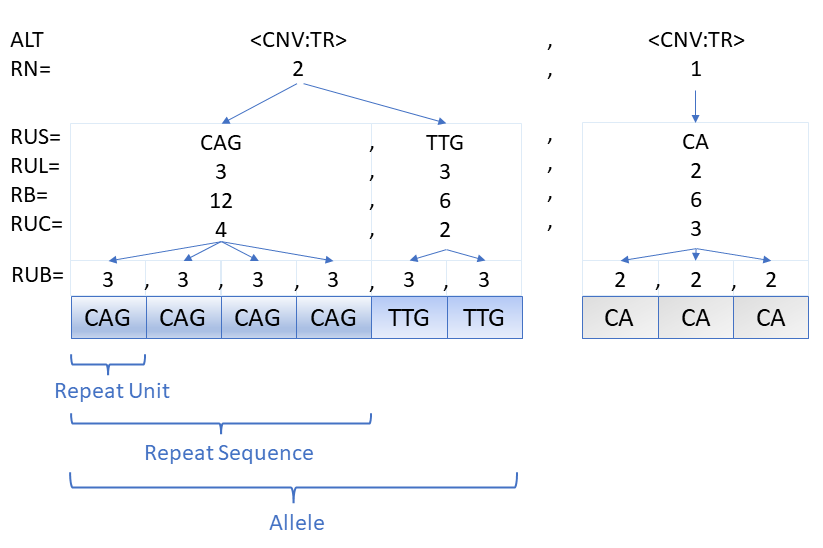
\includegraphics[width=4in,height=2.58in]{img/tandem_repeat_notation.png}
	\caption{$<$CNV:TR$>$ Tandem Repeats}
\end{figure}


A tandem repeat allele can be described by both a $<$CNV:TR$>$ 'summary' record as well as non-symbolic records.
When possible, these records should be phased with their corresponding $<$CNV:TR$>$ record as outlined in the following example.
In the following example, the reference genome contains a $(CAG)_{10}$ repeat at positions 101 to 130 inclusive, the first allele expands this to $(CAG)_{30}$ and the second allele is missing a $G$ from the 6th repeat unit $(CAG)_{5}(CA)_{1}(CAG)_{4}$:

\pagebreak
\footnotesize
\begin{landscape}
\begin{verbatim}
##fileformat=VCFv4.5
##INFO=<ID=END,Number=1,Type=Integer,Description="End position of the longest variant described in this record">
##INFO=<ID=SVLEN,Number=A,Type=Integer,Description="Length of structural variant">
##INFO=<ID=CN,Number=A,Type=Float,Description="Copy number of allele">
##INFO=<ID=RN,Number=A,Type=Integer,Description="Total number of repeat sequences in this allele">
##INFO=<ID=RUS,Number=.,Type=String,Description="Repeat unit sequence of the corresponding repeat sequence">
##INFO=<ID=RUL,Number=.,Type=Integer,Description="Repeat unit length of the corresponding repeat sequence">
##INFO=<ID=RUC,Number=.,Type=Float,Description="Repeat unit count of corresponding repeat sequence">
##INFO=<ID=RB,Number=.,Type=Integer,Description="Total number of bases in the corresponding repeat sequence">
##INFO=<ID=CIRUC,Number=.,Type=Float,Description="Confidence interval around RUC">
##INFO=<ID=CIRB,Number=.,Type=Integer,Description="Confidence interval around RB">
##INFO=<ID=RUB,Number=.,Type=Integer,Description="Number of bases in each individual repeat unit">
##FORMAT=<ID=GT,Number=1,Type=String,Description="Genotype">
##FORMAT=<ID=PS,Number=1,Type=Integer,Description="Phase set">
##FORMAT=<ID=CN,Number=1,Type=Float,Description="Copy number">
##ALT=<ID=CNV:TR,Description="Tandem repeat determined based on DNA abundance">
#CHROM POS ID REF ALT QUAL FILTER INFO FORMAT sample
chr1 100 cnv_notation T <CNV:TR>,<CNV:TR> . . END=130;SVLEN=30,30;CN=3,0.9666;RUS=CAG,CAG,CA,CAG;RN=1,3;RB=90,15,2,12  GT:PS:CN 1|2:100:3.9666
chr1 117 precise_alt2 AG A . . GT:PS 0|1:100
chr1 130 precise_alt1 G GCAGCAGCAGCAGCAGCAGCAGCAGCAGCAGCAGCAGCAGCAGCAGCAGCAGCAGCAGCAG . . GT:PS 1|0:100
\end{verbatim}
\end{landscape}
\pagebreak
\normalsize

Note the following:
\begin{itemize}
    \item As with all symbolic structural variant alleles, the POS of the $<$CNV:TR$>$ record is the base immediately preceding the tandem repeat
    \item The SVLEN of the $<$CNV:TR$>$ is the length of the reference allele.
    It is not the length of the $<$CNV:TR$>$ allele.
    \item The SVLEN of the $<$CNV:TR$>$ allele of a novel (with respect to the reference) tandem repeat should be 1.
    \item The POS of the $<$CNV:TR$>$ allele of a novel (with respect to the reference) tandem repeat should be the base immediately preceding the inserted tandem repeat sequence.
    \item Both a $<$CNV:TR$>$ and one or more non-symbolic records encoding the tandem repeat can be present.
    \item $<$CNV:TR$>$ and the non-symbolic records encoding the tandem repeat should be phased if possible.
    \item When both $<$CNV:TR$>$ and the equivalent non-symbolic records are present, the $<$CNV:TR$>$ should approximately encode the sequence but is not required to encode the sequence exactly.
	For example, SNVs and indels may be omitted in the $<$CNV:TR$>$ record.
    \item Variant callers which do not report allele-specific tandem repeats should use a single $<$CNV:TR$>$ ALT allele and the missing genotype for the GT field (for example, $./.$ if diploid).
    \item The INFO and FORMAT CN fields should be present for $<$CNV:TR$>$ records (as they are $<$CNV$>$ records) and, when present, must correspond to the sample allelic length divided by the reference allelic length.
	Note that CN FORMAT field represents the overall copy number and the INFO CN the allele-specific copy number.
    \item When benchmarking tandem repeats, the $<$CNV:TR$>$ interval provides a region over which a set of (preferably phased) non-symbolic records can be compared against for length and sequence composition.
    \item RN encodes the number of records for each allele in the RUS, RUL, RUC, RB fields.
	Conceptually, this a mechanism to encode a list-of-list with flat list format used in VCF.
    \item STRs should use RUS, whereas VNTRs should use RUL to ensure the VCF records are not excessively large.
    \item RUL should be omitted when RUS is present (as it is redundant when RS is present).
    \item RUS or RUL must be specified for each $<$CNV:TR$>$.
    \item Support for multiple levels of repeat nesting (such as STRs within VNTRs) is limited to the RUL repeat unit length field which allows the overall length of each top-level repeat unit to be encoded.
    \item The POS and END of $<$CNV:TR$>$ records should match the STR/VNTR reference catalog sizes for catalog-based callers.
    \item Variant normalisation has limited utility in regions of low complexity as almost identical haplotypes can have very different normalised representations.
\end{itemize}

In some cases, it is desirable to report the full repeat sequence of all alleles at a given repeat locus in a single VCF records.
There are no restrictions on doing so and in the above example, instead of reporting $precise\_alt1$ and $precise\_alt2$, the variants can be represented directly in a single record with a $REF$ of:
\scriptsize
\begin{verbatim}
CAGCAGCAGCAGCAGCAGCAGCAGCAGCAG
\end{verbatim}
\normalsize
and an $ALT$ of:
\scriptsize
\begin{verbatim}
CAGCAGCAGCAGCAGCAGCAGCAGCAGCAGCAGCAGCAGCAGCAGCAGCAGCAGCAGCAGCAGCAGCAGCAGCAGCAGCAGCAGCAGCAG,CAGCAGCAGCAGCAGCACAGCAGCAGCAG
\end{verbatim}
\normalsize

When the length or number of repeat units in a repeat sequence cannot be determined precisely, CIRB and/or CIRUC can be used to define the bounds.
For example, if the total number of $CAG$ repeats at the above locus was at least 50 ($(CAG)_{50-}$) and the mostly likely number of repeats was 65, then the $<$CNV:TR$>$ could be encoded as follows:

\footnotesize
\begin{verbatim}
chr1 100 . T <CNV:TR> . . END=130;SVLEN=30;CN=6.5;RUS=CAG;RUC=65;CIRUC=-15,. GT ./.
\end{verbatim}
\normalsize

Note that:
\begin{itemize}
	\item RN was omitted as it is only required if at least one $<$CNV:TR$>$ allele has RN greater than 1.
	\item The confidence interval bounds are relative to the nominal value.
	\item A missing upper bound indicates the maximum length is not known.
\end{itemize}

Exactly representing nested repeats results in the loss of some repeat information when representing with a $<$CNV:TR$>$ record.
For repeats such as $((ACCGGC)_{4}(ACCAGT))_{3-5}$, summarising the repeat structure in a $<$CNV:TR$>$ record requires either unrolling the inner repeats, or treating each outer repeat as a separate repeat sequence (the full repeat structure can be stored in a caller-specific non-standard INFO field).
For many VNTRs, the critical information to retain is the length of each repeat unit.
This length information can be encoded in the RUB field.
For example, a 10,000bp VNTRs domain repeated 5 times, each repeat 500bp longer than the previous can be encoded as follows:

\footnotesize
\begin{verbatim}
chr1 1000000 . T <CNV:TR> . . END=20000;SVLEN=20000;CN=1.25;RUL=10000;RUC=5;RUB=10000,10500,11000,11500,12000 GT ./.
\end{verbatim}
\normalsize


	
	
\pagebreak
\section{BCF specification}

VCF is very expressive, accommodates multiple samples, and is widely used in the community.
Its biggest drawback is that it is big and slow.
Files are text and therefore require a lot of space on disk.
A normal batch of a hundred exomes is a few GB, but large-scale VCFs with thousands of exome samples quickly become hundreds of GBs.
Because the file is text, it is extremely slow to parse.

Overall, the idea behind is BCF2 is simple.
BCF2 is a binary, compressed equivalent of VCF that can be indexed with tabix and can be efficiently decoded from disk or streams.
For efficiency reasons BCF2 only supports a subset of VCF, in that all info and genotype fields must have their full types specified.
That is, BCF2 requires that if e.g.\ an info field {\tt AC} is present then it must contain an equivalent VCF header line noting that {\tt AC} is an allele indexed array of type integer.

\subsection{Overall file organization}

A BCF2 file is composed of a mandatory header, followed by a series of BGZF compressed blocks of binary BCF2 records.
The BGZF blocks allow BCF2 files to be indexed with tabix.

BGZF blocks are composed of a VCF header with a few additional records and a block of records.
Following the last BGZF BCF2 record block is an empty BGZF block (a block containing zero type of data), indicating that the records are done.

A BCF2 header follows exactly the specification as VCF, with a few extensions/restrictions:
\begin{itemize}
  \item All BCF2 files must have fully specified contigs definitions.
  No record may refer to a contig not present in the header itself.

  \item All INFO and GENOTYPE fields must be fully typed in the BCF2 header to enable type-specific encoding of the fields in records.
  An error must be thrown when converting a VCF to BCF2 when an unknown or not fully specified field is encountered in the records.
\end{itemize}

\subsection{Header}

The BCF2 header contains the following items:

\vspace{0.3cm}
{\small
\begin{tabular}{|l | l | p{30em} | } \hline
\textbf{Field} & \textbf{Type} & \textbf{Notes} \\ \hline
magic          & char[3]     & The characters ``{\tt BCF}'' \\ \hline
major\_version & uint8\_t    & 2 \\ \hline
minor\_version & uint8\_t    & 2 \\ \hline
l\_text        & uint32\_t   & Length of the ``text'' field, including the terminating NUL character \\ \hline
text           & char[l\_text] & VCF format header text, NUL-terminated \\ \hline
\end{tabular}}
\vspace{0.3cm}

The ``magic'' field and version numbers can be used to quickly examine the file to determine that it's a BCF2.2 file.
The ``text'' field contains the standard VCF header lines in text format, from \verb|##fileformat|
to \verb|#CHROM ...| inclusive, terminated by a NUL character.

Because the type is encoded directly in the header, the recommended extension for BCF2 formatted files is {\sl .bcf}.
BCF2 supports encoding values in a dictionary of strings.
The string map is provided by the keyword \verb|##dictionary=S0,S1,...,SN| as a comma-separate ordered list of strings.
See the ``Dictionary of strings'' section for more details.

\subsubsection{Dictionary of strings}

Throughout the BCF file most string values are be specified by integer reference to their dictionary values.
For example, the following VCF record:
\small
\begin{verbatim}
##INFO=<ID=ASP,Number=0,Type=Flag,Description="X">
##INFO=<ID=RSPOS,Number=1,Type=Integer,Description="Y">
##INFO=<ID=dbSNPBuildID,Number=1,Type=Integer,Description="Z">
##contig=<ID=20,length=62435964,assembly=B36,md5=f126cdf8a6e0c7f379d618ff66beb2da,species="Homo sapiens">
#CHROM POS ID REF ALT QUAL FILTER INFO
20 10144 rs144773400 TA T . PASS ASP;RSPOS=10145,dbSNPBuildID=134
20 10228 rs143255646 TA T . PASS ASP;RSPOS=10229;dbSNPBuildID=134
\end{verbatim}
\normalsize
would be encoded inline in BCF2 by reference to the relative position of the header line in the header (ASP=1, RSPOS=2, dbSNPBuildID=3, and PASS implicitly encoded in the first offset PASS=0).

\small
\begin{verbatim}
##INFO=<ID=ASP,Number=0,Type=Flag,Description="X">
##INFO=<ID=RSPOS,Number=1,Type=Integer,Description="Y">
##INFO=<ID=dbSNPBuildID,Number=1,Type=Integer,Description="Z">
##contig=<ID=20,length=62435964,assembly=B36,md5=f126cdf8a6e0c7f379d618ff66beb2da,species="Homo sapiens">
#CHROM POS ID REF ALT QUAL FILTER INFO
0 10144 rs144773400 TA T . s0 s1;s2=10145;s3=134
0 10228 rs143255646 TA T . s0 s1;s2=10229;s3=134
\end{verbatim}
\normalsize

Defined this way, the dictionary of strings depends on the order and the presence of all preceding header lines.
If an existing tag needs to be removed from a BCF, also all consequent tags throughout the whole BCF would have to be recoded.
In order to avoid this costly operation, a new IDX field can be used to explicitly define the position which is dropped on BCF-to-VCF conversion.
If not present, the implicit relative position is assumed.
If the IDX field is present in one record, it must be present also in all other dictionary-defining records.
The IDX tag is not necessary in newly created BCF files, but if present, the numbering must match the implicit dictionary of tags.

Note that the dictionary encoding has the magic prefix `s' here to indicate that the field's value is actually in the dictionary entry giving by the subsequent offset.
This representation isn't actually the one used in BCF2 records but it provides a clean visual guide for the above example.
Note also how the contig has been recoded as a offset into the list of contig declarations.

Note that ``PASS'' is always implicitly encoded as the first entry in the header dictionary.
This is because VCF allows FILTER fields to be PASS without explicitly listing this in the FILTER field itself.


\subsubsection{Dictionary of contigs}

The CHROM field in BCF2 is encoded as an integer offset into the list of \verb|##contig| field headers in the VCF header.
The offsets begin, like the dictionary of strings, at 0.
So for example if in BCF2 the contig value is 10, this indicates that the actual chromosome is the 11th element in the ordered list of \verb|##contig| elements.
Here's a more concrete example:

\small
\begin{verbatim}
##contig=<ID=20,length=62435964,assembly=B36,md5=f126cdf8a6e0c7f379d618ff66beb2da,species="Homo sapiens">
##contig=<ID=21,length=46944323,assembly=B36,md5=f1b74b7f9f4cdbaeb6832ee86cb426c6,species="Homo sapiens">
##contig=<ID=22,length=49691432,assembly=B36,md5=2041e6a0c914b48dd537922cca63acb8,species="Homo sapiens">
#CHROM POS ID REF ALT QUAL FILTER INFO
20 1 . T A . PASS .
21 2 . T A . PASS .
22 3 . T A . PASS .
\end{verbatim}
\normalsize

the actual CHROM field values in the encoded BCF2 records would be 0, 1, and 2 corresponding to the first (offset 0) \verb|##contig| element, etc.

\subsection{BCF2 records}

In BCF2, the original VCF records are converted to binary and encoded as BGZF blocks.
Each record is conceptually two parts.
First is the site information (chr, pos, INFO field).
Immediately after the sites data is the genotype data for every sample in the BCF2 file.
The genotype data may be omitted entirely from the record if there is no genotype data in the VCF file.
Compression of a BCF file is recommended but not required.

\subsubsection{Site encoding}
\label{BcfSiteEncoding}

{\small
\begin{tabular}{|l | l | p{30em} | } \hline
\textbf{Field} &	\textbf{Type} &	\textbf{Notes} \\ \hline
l\_shared & uint32\_t & Data length from CHROM to the end of INFO \\ \hline
l\_indiv  & uint32\_t & Data length of FORMAT and individual genotype fields \\ \hline
CHROM     & int32\_t  & Given as an offset into the mandatory contig dictionary \\ \hline
POS       & int32\_t  & 0-based leftmost coordinate \\ \hline
rlen      & int32\_t  & Length of the record as projected onto the reference sequence.
                        Must be the maximum of the length of the REF allele and the lengths
                        inferred from the SVLEN/END of any symbolic alleles \\ \hline
QUAL      & float     & Variant quality; 0x7F800001 for a missing value \\ \hline
n\_info   & uint16\_t & The number of INFO fields in this record \\ \hline
n\_allele & uint16\_t & The number of REF+ALT alleles in this record \\ \hline
n\_sample & uint24\_t & The number of samples in this record, stored as a \textbf{three} byte little-endian value.
                        Note that n\_sample must be equal to the number of samples in the header \\ \hline
n\_fmt    & uint8\_t  & The number of FORMAT keys.  See \ref{GenotypeEncoding} \\ \hline
ID       & typed string & Variant identifier; 0x07 for a missing value \\ \hline
REF+ALT  & list of n\_allele typed strings & the first allele is REF (mandatory) followed by n\_alleles - 1 ALT
                                             alleles, all encoded as typed strings \\ \hline
FILTER   & Typed vector of integers & a vector of integer offsets into dictionary, one for each FILTER field value.
                                      ``.'' is encoded as MISSING \\ \hline
INFO     & field key/value pairs & n\_info pairs of typed vectors.
                                   The first value must be a typed atomic integer giving the offset of the INFO field
                                   key into the dictionary.
                                   The second value is a typed vector giving the value of the field \\ \hline
Genotype values & see below & see below \\ \hline
\end{tabular}}

\subsubsection{Genotype encoding}
\label{GenotypeEncoding}

Genotype fields are encoded not by sample as in VCF but rather by field, with a vector of values for each sample following each field.
In BCF2, the following VCF line:

\vspace{0.3cm}
\begin{tabular}{l l l l}
FORMAT & NA00001 & NA00002 & NA00003 \\
GT:GQ:DP & 0/0:48:1 & 0/1:9:8 & 1/1:43:5 \\
\end{tabular}
\vspace{0.3cm}

would encoded as the equivalent of:

\vspace{0.3cm}
\begin{tabular}{l l l l}
GT=0/0,0/1,1/1 & GQ=48,9,43 & DP=1,8,5
\end{tabular}
\vspace{0.3cm}

Suppose there are i genotype fields in a specific record.
Each i is encoded by a triplet:

BCF2 site information encoding

\vspace{0.3cm}
\small
\begin{tabular}{ | p{2cm} | p{2.5cm} | p{9.5cm} | } \hline
Field & Type & Notes \\ \hline
fmt\_key & typed int & Format key as an offset into the dictionary \\ \hline
fmt\_type & uint8\_t+ & Typing byte of each individual value, possibly followed by a typed int for the vector length.  
In effect this is the same as the typing value for a single vector, but for genotype values it appears only once before the array of genotype field values \\ \hline
\makecell[tl]{fmt\_values \\ (by fmt type)} & Array of values & The information of each individual is concatenated in the vector.  Every value is of the same fmt type.
Variable-length vectors are padded with END\_OF\_VECTOR values; a string is stored as a vector of char \\  \hline
\end{tabular}
\normalsize
\vspace{0.3cm}

The value is always implicitly a vector of N values, where N is the number of samples.
The type byte of the value field indicates the type of each value of the N length vector.
For atomic values this is straightforward (size = 1).
But if the type field indicates that the values are themselves vectors (as often occurs, such as with the PL field) then each of the N values in the outer vector is itself a vector of values.
This encoding is efficient when every value in the genotype field vector has the same length and type.

It is recommended to respect the ordering as specified in the input VCF/BCF2 file, but parsers should not rely on a specific ordering.

If there are no sample records (genotype data) in this VCF/BCF2 file, the size of the genotypes block will be 0.


\subsubsection{Type encoding}
\label{BcfTypeEncoding}

In BCF2 values are all strongly typed in the file.
The type information is encoded in a prefix byte before the value, which contains information about the low-level type of the value(s) such as int32 or float, as well as the number of elements in the value.
The encoding is as follows:

\vspace{0.3cm}
\textbf{BCF2 type descriptor byte}

\vspace{0.3cm}
\begin{tabular}{|p{2cm} | p{10cm}|} \hline
Bit & Meaning \\ \hline
5,6,7,8 bits & The number of elements of the upcoming type. 
For atomic values, the size must be 1. 
If the size is set to 15, this indicates that the vector has 15 or more elements, and that the subsequent BCF2 byte stream contains a typed Integer indicating the true size of the vector. 
If the size is between 2--14, then this Integer is omitted from the stream and the upcoming stream begins immediately with the first value of the vector.
A size of 0 indicates that the value is MISSING. \\ \hline
1,2,3,4 bits & Type \\ \hline
\end{tabular}
\vspace{0.3cm}

The final four bits encodes an unsigned integer that indicates the type of the upcoming value in the data stream.

\textbf{BCF2 types}

\vspace{0.3cm}
\begin{tabular}{|l | l | l|} \hline
Lowest 4 bits & Hexadecimal encoding & Corresponding atomic type \\ \hline
0 & 0x00 & A MISSING value without an explicit type provided \\ \hline
1 & 0x?1 & Integer [8 bit] \\ \hline
2 & 0x?2 & Integer [16 bit] \\ \hline
3 & 0x?3 & Integer [32 bit] \\ \hline
5 & 0x?5 & Float [32 bit] \\ \hline
7 & 0x?7 & Character, ASCII encoded in 8 bits \\ \hline
\end{tabular}
\vspace{0.3cm}

In BCF2 strings are type=7 with an appropriate length.
Single characters are represented as strings with length=1.
Type codes 4,6,8--15 are reserved for future use.

\vspace{0.3cm}

\textbf{Integers} may be encoded as 8, 16, or 32 bit values, in little-endian order.
It is up to the encoder to determine the appropriate ranged value to use when writing the BCF2 file.
For integer types, the values 0x80, 0x8000, 0x80000000 are interpreted as missing values and 0x81, 0x8001, 0x80000001 as END\_OF\_VECTOR indicators (for 8, 16, and 32 bit values, respectively).
Note that the END\_OF\_VECTOR byte is not part of the vector itself and only END\_OF\_VECTOR bytes can follow.
In total, eight values are reserved for future use: 0x80--0x87, 0x8000--0x8007, 0x80000000--0x80000007.

\vspace{0.3cm}
\textbf{Floats} are encoded as single-precision (32 bit) in the basic format defined by the IEEE-754-1985 standard.
This is the standard representation for floating point numbers on modern computers, with direct support in programming languages like C and Java (see Java's Double class for example).
BCF2 supports the full range of values from -Infinity to +Infinity, including NaN.
BCF2 needs to represent missing values for single precision floating point numbers.
This is accomplished by writing the NaN value as the quiet NaN (qNaN), while the MISSING value is encoded as a signaling NaN.
From the NaN wikipedia entry, we have:

\begin{quote}
For example, a bit-wise example of a IEEE floating-point standard single precision (32-bit) NaN would be: s111 1111 1axx xxxx xxxx xxxx xxxx xxxx where s is the sign (most often ignored in applications), a determines the type of NaN, and x is an extra payload (most often ignored in applications).
If a = 1, it is a quiet NaN; if a is zero and the payload is nonzero, then it is a signaling NaN.
\end{quote}

\noindent A good way to understand these values is to play around with the IEEE encoder website.

\vspace{0.3cm}
\noindent Similarly to integers, the float value of 0x7F800001 is interpreted as a MISSING value and 0x7F800002 as the END\_OF\_VECTOR indicator. 
Note that the END\_OF\_VECTOR byte is not part of the vector itself and only END\_OF\_VECTOR bytes can follow.
In total, eight values are reserved for future use:


\vspace{0.1cm}
\begin{tabular}{| l | c | l |} \hline
\textbf{Value}   & \textbf{32-bit precision} & \textbf{Hexadecimal representation} \\ \hline
NaN	    & 0b0111 1111 1100 0000 0000 0000 0000 0000 & 0x7FC00000 \\ \hline
MISSING & 0b0111 1111 1000 0000 0000 0000 0000 0001 & 0x7F800001 \\ \hline
END\_OF\_VECTOR & 0b0111 1111 1000 0000 0000 0000 0000 0010 & 0x7F800002 \\ \hline
reserved & 0b0111 1111 1000 0000 0000 0000 0000 0011 & 0x7F800003 \\ \hline
$\ldots$ & $\ldots$ & $\ldots$ \\ \hline
reserved & 0b0111 1111 1000 0000 0000 0000 0000 0111 & 0x7F800007 \\ \hline
\end{tabular}

\vspace{0.3cm}
\textbf{Character} values are not explicitly typed in BCF2.
Instead, VCF Character values must be encoded by a single character string. See also \ref{character-encoding}.

\vspace{0.3cm}
\textbf{Flags} values --- which can only appear in INFO fields --- in BCF2 should be encoded by any non-reserved value.
The recommended best practice is to encode the value as an 1-element INT8 (type 0x11) with value of 1 to indicate present.
Because FLAG values can only be encoded in INFO fields, BCF2 provides no mechanism to encode FLAG values in genotypes, but could be easily extended to do so if allowed in a future VCF version.

\vspace{0.3cm}
\textbf{String} values have two basic encodings.
For INFO, FORMAT, and FILTER keys these are encoded by integer offsets into the header dictionary.
For string values, such as found in the ID, REF, ALT, INFO, and FORMAT fields, strings are encoded as typed array of ASCII encoded bytes.
The array isn't terminated by a NUL byte.
The length of the string is given by the length of the type descriptor.

Suppose you want to encode the string ``{\tt ACAC}''.
First, we need the type descriptor byte, which is the string type 0x07 or'd with inline size (4) yielding the type byte of 0x40 $|$ 0x07 = 0x47.
Immediately following the type byte is the four byte ASCII encoding of ``{\tt ACAC}'': 0x41 0x43 0x41 0x43.
So the final encoding is:

\vspace{0.1cm}
\begin{tabular}{| l | l |} \hline
0x47 0x41 0x43 0x41 0x43 & String type with inline size of 4 followed by ACAC in ASCII \\ \hline
\end{tabular}
\vspace{0.3cm}

Suppose you want to encode the string ``{\tt VariantCallFormatSampleText}'', a string of size 27.
First, we need the type descriptor byte, which is the string type 0x07.
Because the size exceeds the inline size limit ($27 \geq 15$) we set the size to overflow, yielding the type byte of 0xF0 $|$ 0x07 = 0xF7.
Immediately following the type byte is the typed size of 27, which we encode by the atomic INT8 value: 0x11 followed by the actual size 0x1B.
Finally comes the actual bytes of the string: 0x56 0x61 0x72 0x69 0x61 0x6E 0x74 0x43 0x61 0x6C 0x6C 0x46 0x6F 0x72 0x6D 0x61 0x74 0x53 0x61 0x6D 0x70 0x6C 0x65 0x54 0x65 0x78 0x74.
So the final encoding is:

\vspace{0.3cm}
\begin{tabular}{ | p{9cm} | p{6cm} | } \hline
0xF7 & string with overflow size \\ \hline
0x11 0x1B & overflow size encoded as INT8 with value 27 \\ \hline
0x56 0x61 0x72 0x69 0x61 0x6E 0x74 0x43 0x61 0x6C 0x6C 0x46 0x6F 0x72 0x6D 0x61 0x74 0x53 0x61 0x6D 0x70 0x6C 0x65 0x54 0x65 0x78 0x74 & message in ASCII \\ \hline
\end{tabular}
\vspace{0.3cm}

Suppose you want to encode the missing value `.'.
This is simply a string of size 0 = 0x07.

\vspace{0.3cm}
In VCF there are sometimes fields of type list of strings, such as a number field of unbounded size encoding the amino acid changes due to a mutation.
Since BCF2 doesn't directly support vectors of strings (a vector of character is already a string) we collapse the list of strings into a single comma-separated string, encode it as a regular BCF2 vector of characters, and on reading explode it back into the list of strings.
This works because strings in VCF cannot contain `{\tt ,}' (it's a field separator) and so we can safely use `{\tt ,}' to separate the individual strings.

% String vectors in BCF do not need to start with comma, as the number of
% values is indicated already in the definition of the tag in the header.
%
% For efficiency
% reasons we put a comma at the start of the collapsed string, so that just the
% first character can be examined to determine if the string is collapsed.
%END\_OF\_VECTOR
% To be concrete, suppose we have a info field around X=[A,B,C,D].  This is
% encoded in BCF2 as a single string ``,A,B,C,D'' of size 8, so it would have
% type byte 0x87 followed by the ASCII encoding 0x2C 0x41 0x2C 0x42 0x2C 0x43
% 0x2C 0x44.

\vspace{0.3cm}

\textbf{Vectors} --- The BCF2 type byte may indicate that the upcoming data stream contains not a single value but a fixed length vector of values.
The vector values occur in order (1st, 2nd, 3rd, etc) encoded as expected for the type declared in the vector's type byte.
For example, a vector of 3 16-bit integers would be laid out as first the vector type byte, followed immediately by 3 2-byte values for each integer, including a total of 7 bytes.

Missing values in vectors are handled slightly differently from atomic values.
There are two possibilities for missing values:

One (or more) of the values in the vector may be missing, but others in the vector are not.
Here each value should be represented in the vector, and each corresponding BCF2 vector value either set to its present value or the type equivalent MISSING value.
Alternatively the entire vector of values may be missing.
In this case the correct encoding is as a type byte with size 0 and the appropriate type MISSING.
Suppose we are encoding the record ``AC=[1,2,3]'' from the INFO field.
The AC key is encoded in the standard way.
This would be immediately followed by a typed 8-bit integer vector of size 3, which is encoded by the type descriptor 0x31.
The type descriptor is immediately followed by the three 8-bit integer values: 0x01 0x02 0x03, for a grand total of 4 bytes: 0x31010203.

Suppose we are at a site with many alternative alleles so AC=[1,2,3,4,5,6,7,8,9,10,11,12,13,14,15,16].
Since there are 16 values, we have to use the long vector encoding.
The type of this field is 8 bit integer with the size set to 15 to indicate that the size is the next stream value, so this has type of 0xF1.
The next value in the stream is the size, as a typed 8-bit atomic integer: 0x11 with value 16 0x10.
Each integer AC value is represented by it's value as a 8 bit integer.
The grand total representation here is:

\vspace{0.3cm}
\begin{tabular}{|p{9cm} | p{6cm}|} \hline
0xF1 0x01 0x10 & 8 bit integer vector with overflow size \\ \hline
0x01 0x02 0x03 0x04 0x05 0x06 0x07 0x08 0x09 0x0A 0x0B 0x0C 0x0D 0x0E 0x0F 0x10 & 1--16 as hexadecimal 8 bit integers \\ \hline
\end{tabular}
\vspace{0.3cm}

Suppose this INFO field contains the ``AC=.'', indicating that the AC field is missing from a record with two alt alleles.
The correct representation is as the typed pair of AC followed by a MISSING vector of type 8-bit integer: 0x01.

\vspace{0.3cm}
\textbf{Vectors of mixed length} --- In some cases genotype fields may be vectors whose length differs among samples.  
For example, some CNV call sets encode different numbers of genotype likelihoods for each sample, given the large number of potential copy number states, rather padding all samples to have the same number of fields.  
For example, one sample could have CN0:0,CN1:10 and another CN0:0,CN1:10,CN2:10.  
In the situation when a genotype field contain vector values of different lengths, these are represented in BCF2 by a vector of the maximum length per sample, with all values in the each vector aligned to the left, and END\_OF\_VECTOR values assigned to all values not present in the original vector.  
The BCF2 encoder / decoder must automatically add and remove these END\_OF\_VECTOR values from the vectors. Note that the use of END\_OF\_VECTOR means that it is legal to encode a vector VCF field with MISSING values.

For example, suppose I have two samples, each with a FORMAT field X.  
Sample A has values [1], while sample B has [2,3].  
In BCF2 this would be encoded as [1, END\_OF\_VECTOR] and [2, 3]. 
Diving into the complete details, suppose X is at offset 3 in the dictionary, which is encoded by the typed INT8 descriptor 0x11 followed by the value 0x03. 
Next we have the type of the each format field, which here is a 2 element INT8 vector: 0x21.  
Next we have the encoding for each sample, A = 0x01 0x81 followed by B = 0x02 0x03.  
All together we have:

\vspace{0.3cm}
\begin{tabular}{|p{2cm} | l |} \hline
0x11 0x03 & X dictionary offset \\ \hline
0x21 & each value is a 2 element INT8 value \\ \hline
0x01 0x81 & A is [1, END\_OF\_VECTOR] \\ \hline
0x02 0x03 & B is [2, 3] \\ \hline
\end{tabular}
\vspace{0.3cm}


\vspace{0.3cm}
A \textbf{Genotype (GT) field} is encoded in a typed integer vector (can be 8, 16, or even 32 bit if necessary) with the number of elements equal to the maximum ploidy among all samples at a site.
For one individual, each integer in the vector is organized as $(allele+1) << 1 \mid phased$ where allele is set to $-1$ if the allele in GT is a dot `.' (thus the higher bits are all 0).
The vector is padded with the END\_OF\_VECTOR values if the GT having fewer ploidy.
We note specifically that except for the END\_OF\_VECTOR byte, no other negative values are allowed in the GT array.
When processing VCF version 4.3 or earlier files, the phasing of the first allele should be treated as missing and inferred from the remaining alleles.

Examples:

\vspace{0.3cm}
\small
\begin{tabular}{|p{2.5cm} | p{10cm} | p{3cm}|} \hline
0/1 & in standard format $(0 + 1) << 1 \mid 0$ followed by $(1 + 1) << 1 \mid 0$ & 0x02 04 \\ \hline
0/1, 1/1, and 0/0 & three samples encoded consecutively & 0x02 04 04 04 02 02 \\ \hline
$0\mid1$ & $(1 + 1) << 1 \mid 1$ = 0x05 preceded by the standard first byte value 0x02 & 0x02 05 \\ \hline
./. & where both alleles are missing & 0x00 00 \\ \hline
0 & as a haploid it is represented by a single byte & 0x02 \\ \hline
1 & as a haploid it is represented by a single byte & 0x04 \\ \hline
0/1/2 & is tetraploid, with alleles & 0x02 04 06 \\ \hline
$0/1\mid2$ & is tetraploid with a single phased allele & 0x02 04 07 \\ \hline
0 and 0/1 & pad out the final allele for the haploid individual & 0x02 81 02 04\\ \hline
\end{tabular}
\normalsize

\vspace{0.3cm}
The final example is something seen on chrX when we have a haploid male and a diploid female.
The male genotype vector is terminated prematurely by the END\_OF\_VECTOR value.
\vspace{0.3cm}


\subsection{Encoding a VCF record example}

Let's encode a realistic (but made-up) VCF record.
This is a A/C SNP in HM3 (not really) called in~3 samples.
In this section we'll build up the BCF2 encoding for this record.
\scriptsize
\begin{verbatim}
#CHROM POS ID REF ALT QUAL FILTER INFO FORMAT NA00001 NA00002 NA00003
chr1 101 rs123 A C 30.1 PASS HM3;AC=3;AN=6;AA=C GT:GQ:DP:AD:PL 0/0:10:32:32,0:0,10,100 0/1:10:48:32,16:10,0,100 1/1:10:64:0,64:100,10,0
\end{verbatim}
\normalsize

\subsubsection{Encoding CHROM and POS}

First, let's assume that {\tt chr1} is the second chromosome to appear in the contig list---right after {\tt chrM} ({\tt MT}).
So its offset is 1.
The {\tt POS} BCF2 field value is~101 (obviously).
Because these are both typed values in the BCF2 record, we encode both in their most compact 8-bit value form.
The type byte for an atomic 8-bit integer is 0x11.
The value for the contig offset is 1 = 0x01.
The value 101 is encoded as the single byte 0x65.
So in total these are represented as:

\vspace{0.3cm}
\begin{tabular}{|l | l|} \hline
0x01000000 & CHROM offset is at 1 in 32 bit little endian \\ \hline
0x64000000 & POS in 0 base 32 bit little endian \\ \hline
0x01000000 & rlen = 1 (it's just a SNP) \\ \hline
\end{tabular}

\subsubsection{Encoding QUAL}

The QUAL field value is 30.1, which we encode as an untyped single precision 32-bit float:

\vspace{0.3cm}
\begin{tabular}{|l| l|} \hline
0x41 0xF0 0xCC 0xCD & QUAL = 30.1 as 32-bit float \\ \hline
\end{tabular}

\subsubsection{Encoding ID}

This ID value is a 5-element string, so is encoded as type descriptor 0x57 followed by the five bytes for the string of {\tt 0x72 0x73 0x31 0x32 0x33}.
The full encoding is:

\vspace{0.3cm}
\begin{tabular}{|l| l|} \hline
0x57 0x72 0x73 0x31 0x32 0x33 & ID = rs123 \\ \hline
\end{tabular}

\subsubsection{Encoding REF/ALT fields}

We encode each of REF and ALT as typed strings, first REF followed immediately by ALT.
Each is a 1 element string (0x17), which would then be followed by the single bytes for the bases of 0x43 and 0x41:

\vspace{0.3cm}
\begin{tabular}{|l| l|} \hline
0x17 0x41 & REF A \\ \hline
0x17 0x43 & ALT C \\ \hline
\end{tabular}

\vspace{0.3cm}
Just for discussion, suppose instead that ALT was ALT=C,T.
The only thing that could change is that there would be another typed string following immediately after C encoding 0x17 (1 element string) with the value of 0x54.

\subsubsection{Encoding FILTER}

``PASS'' is implicitly encoded as the first entry in the header dictionary (see dictionary of strings).
Here we encode the PASS FILTER field as a vector of size 1 of type 8-bit, which has type byte is 0x11.
The value is the offset 0:

\vspace{0.3cm}
\begin{tabular}{|l| l|} \hline
0x11 0x00 & FILTER field PASS \\ \hline
\end{tabular}

\subsubsection{Encoding the INFO fields}

HM3;AC=3;AN=6;AA=C
Let's assume that the header dictionary elements for HM3, AC, AN, and AA are at 80, 81, 82, and 83 respectively.
All of these can be encoded by 1-element INT8 values (0x11), with associated hex values of 0x50, 0x51, 0x52, and 0x53 respectively.

First is HM3.
The entry begins with the key: 0x11 0x50.
The HM3 field is a flag with no associated value and therefore the rest of the entry is the special case of a missing value without an explicit type provided.
Altogether we have:

\vspace{0.3cm}
\begin{tabular}{|l| l|} \hline
0x11 0x50 0x00 & HM3 flag is present \\ \hline
\end{tabular}
\vspace{0.3cm}

Now let's encode the two atomic 8-bit integer fields AC and AN:

\vspace{0.3cm}
\begin{tabular}{|l| l|} \hline
0x11 0x51 & AC key \\ \hline
0x11 0x03 & with value of 3 \\ \hline
0x11 0x52 & AN key \\ \hline
0x11 0x06 & with value of 6 \\ \hline
\end{tabular}
\vspace{0.3cm}

The ancestral allele (AA) tell us that among other primates the original allele is C, a Character here.
Because we represent Characters as single element strings in BCF2 (0x17) with value 0x43 (C).
So the entire key/value pair is:

\vspace{0.3cm}
\begin{tabular}{|l |l|} \hline
0x11 0x53 & AA key \\ \hline
0x17 0x43 & with value of C \\ \hline
\end{tabular}

\subsubsection{Encoding Genotypes}

Continuing with our example:

\vspace{0.3cm}
\begin{tabular}{l l l l}
FORMAT & NA00001 & NA00002 & NA00003 \\
GT:GQ:DP:AD:PL & 0/0:10:32:32,0:0,10,100 & 0/1:10:48:32,16:10,0,100 & 1/1:10:64:0,64:100,10,0 \\
\end{tabular}
\vspace{0.3cm}

Here we have the specially encoded GT field.
We have two integer fields GQ and DP.
We have the AD field, which is a vector of 2 values per sample.
And finally we have the PL field which is 3 values per sample.
Let's say that the FORMAT keys for GT, GQ, DP, AD, and PL are at offsets 1, 2, 3, and 4, 5, respectively.
Now let's encode each of the genotype fields in order of the VCF record (GT, GQ, DP, AD, and then PL):

GT triplet begins with the key: 0x1101.
Next is the type of the field, which will be a 2-element (diploid) INT8 type: 0x21.
This is followed by 3 2-byte arrays of values 0x0202 0x0204 0x0404 (see genotype encoding example for details).
The final encoding is 0x1101 0x21 0x020202040404

GQ triplet begins with the key 0x1102.
Because these values are small, we encode them as 8 bit atomic integers with type code 0x11.
As each value is the same (10 = 0x0A) the GQ field is encoded as 0x1102 0x11 0x0A0A0A

DP almost identical to GQ.
First is the 0x1103 key, followed by 3 8-bit atomic integers encoded as 0x11 (the type) 0x20 (DP=32), 0x30 (DP=48) and 0x40 (DP=64).
So we have: 0x1103 0x11203040

AD is more complex.
The key is simple, just like the others, with 0x1104.
Because the AD field is a vector of 2 values for each genotype, the value of key/value pair a vector type.
Because the integer values in each AD field of each sample are small they are encoded by 8 bit values.
So the value type is = 0x21.
For sample one there are two values: 32,0 which are 0x30 and 0x00.
Samples two and three are 0x30 0x20 and 0x00 0x40 respectively.
So ultimately this field is encoded as 0x1104 0x21 0x300030200040

PL is just like AD but with three values per sample.
The key is 0x1105.
Because the PL field is a vector of 3 values for each genotype, the value of key/value pair a vector type, and because the size is 3 it's encoded in the size field of the type.
Again, because the integer values in each PL field of each sample are small they are encoded by 8 bit values.
So the value type 0x31.
For sample one there are three values: 0, 10, and 100 which are 0x00, 0x0A, and 0x64.
Samples two and three have the same values but in a slightly different order.
So ultimately the PL field is encoded as 0x1105 0x31 0x000A64 0x0A0064 0x640A00

So the genotype block contains:

\vspace{0.3cm}
\begin{tabular}{|l| l|} \hline
0x1101 0x21 0x020202040404 & GT \\ \hline
0x1102 0x11 0x0A0A0A & GQ \\ \hline
0x1103 0x11 0x203040 & DP \\ \hline
0x1104 0x21 0x300030200040 & AD \\ \hline
0x1105 0x31 0x000A640A0064640A00 & PL \\ \hline
\end{tabular}
\vspace{0.3cm}

\textbf{Putting it all together}

We need to determine a few values before writing out the final block:

l\_shared = 51 (Data length from CHROM to the end of INFO)

l\_indiv = 42 (Data length of FORMAT and individual genotype fields)

n\_info = 4 (Number of INFO fields)

n\_allele = 2 (Number of alleles, including REF)

n\_sample = 3 (Number of samples)

n\_fmt = 5 (Number of FORMAT keys)

\vspace{0.3cm}
\begin{tabular}{|l| l|} \hline
0x33000000 & l\_shared as 32-bit little endian hex \\ \hline
0x2A000000 & l\_indiv as 32-bit little endian hex \\ \hline
0x01000000 & CHROM offset is at 1 in 32 bit little endian \\ \hline
0x64000000 & POS in 0-based 32-bit little endian \\ \hline
0x01000000 & rlen = 1 (it's just a SNP) \\ \hline
0x41 0xF0 0xCC 0xCD & QUAL = 30.1 as 32-bit float \\ \hline
0x0400     & n\_info as 16-bit little-endian \\ \hline
0x0200     & n\_allele as 16-bit little-endian \\ \hline
0x030000   & n\_sample as 24-bit little-endian \\ \hline
0x05       & n\_fmt \\ \hline
0x57 0x72 0x73 0x31 0x32 0x33 & ID = rs123 \\ \hline
0x17 0x41 & REF A \\ \hline
0x17 0x43 & ALT C \\ \hline
0x11 0x00 & FILTER field PASS \\ \hline
0x11 0x50 0x00 & HM3 flag is present \\ \hline
0x11 0x51 & AC key \\ \hline
0x11 0x03 & with value of 3 \\ \hline
0x11 0x52 & AN key \\ \hline
0x11 0x06 & with value of 6 \\ \hline
0x11 0x53 & AA key \\ \hline
0x17 0x43 & with value of C \\ \hline
0x1101 0x21 0x020202040404 & GT \\ \hline
0x1102 0x11 0x0A0A0A & GQ \\ \hline
0x1103 0x11 0x203040 & DP \\ \hline
0x1104 0x21 0x300030200040 & AD \\ \hline
0x1105 0x31 0x000A640A0064640A00 & PL \\ \hline
\end{tabular}
\vspace{0.3cm}

That's quite a lot of information encoded in only 96 bytes!

\subsection{BCF2 block gzip and indexing}

These raw binary records may be subsequently encoded into BGZF blocks following the BGZF compression format, section 3 of the SAM format specification.
BCF2 records can be raw, though, in cases where the decoding/encoding costs of bgzipping the data make it reasonable to process the data uncompressed, such as streaming BCF2s through pipes with samtools and bcftools.
Here the files should be still compressed with BGZF but with compression 0.
Implementations should perform BGZF encoding and must support the reading of both raw and BGZF encoded BCF2 files.

BCF2 files are expected to be indexed through the same index scheme, section~4 as BAM files and other block-compressed files with BGZF.

\section{List of changes}

\subsection{Changes between VCFv4.5 and VCFv4.4}

\begin{itemize}
\end{itemize}

\subsection{Changes between VCFv4.4 and VCFv4.3}

\begin{itemize}
\item Added tandem repeat support ($<$CNV:TR$>$, RN, RUS, RUL, RB, CIRB, RUC, CIRUC, RUB)
\item Redefined INFO CN as allele-specific copy number and FORMAT CN as total copy number.
\item Redefined INFO and FORMAT CN to support non-integer copy numbers.
\item Added support for phasing and derivative chromosome reconstruction in the presence of SVs (PSL, PSO, PSQ)
\item Added SVCLAIM to disambiguate copy number based $<$DEL$>$ and $<$DUP$>$ variants from breakpoint based ones.
\item Conceptually separated variant detection and interpretation.
\item Added EVENTTYPE/EVENT to enable the multiple records encoding complex genomic rearrangements to be grouped together.
\item Added polyploid partial phasing support (e.g. GT $|0|0/1/2$). GT now defined as a prefix notation with the first phasing indicator optional.
\item Redefined $Number=$ for SVLEN, CIPOS, CIEND, HOMLEN, HOMSEQ, BKPTID, MEINFO, METRANS, DGVID, DBVARID, DBRIPID, MATEID, PARID, EVENT, CN, CICN to support multiple symbolic alleles.
\item Redefined END as the end position of the longest ALT allele. Note that END remains $Number=1$.
\item Redefined SVLEN to always be positive and be meaningful for INV variants.
\item Redefined SVLEN, END and BCF rlen to support both $<*>$ and symbolic structural variant alleles in the same record.
\item Number, Type and Description required only for INFO meta-information lines
\item Clarified CIPOS should be used to define micro-homology bounds
\item Clarified INFO lines field ordering
\item Clarified that symbolic and breakpoint notation ALT alleles are case sensitive.
\item Deprecated SVTYPE
\item Removed DPADJ, CNADJ, CICNADJ
\item Disallowed BND ALT records (these should use breakpoint notation anyway)
\item Removed definition of DP from Section 3 as it was already defined in Section 1.6.1.8.
\item Deprecated bundles in favour of PSL-based phasing.
\item Updated SV examples.
\item BCF parsers should perform BGZF encoding and must support both raw and BGZF encoded files.
\end{itemize}

\subsection{Changes to VCFv4.3}

\begin{itemize}
\item More strict language: ``should'' replaced with ``must'' where appropriate
\item Tables with Type and Number definitions for INFO and FORMAT reserved keys

\item
The set of characters allowed in VCF contig names is now the same as that allowed in SAM reference sequence names, which was restricted in January 2019.
The characters `{\tt\verb|\|\,,\,"`'\,()\,\verb|{}|}' are now invalid in VCF contig names, while `{\tt *}' is now valid when not the first character.
(The characters `{\tt []\,<>}' and initial~`{\tt *}'/`{\tt =}' were already invalid and remain so.)

The VCF specification previously disallowed colons (`{\tt :}') in contig names to avoid confusion when parsing breakends, but this was unnecessary.
Even with contig names containing colons, the breakend mate position notation can be unambiguously parsed because the ``{\tt :}\emph{pos}'' part is \textbf{always} present.
\item Added PP tag which is the phred-scaled analogue to GP
\end{itemize}

\subsection{Changes between VCFv4.2 and VCFv4.3}

\begin{itemize}
\item VCF compliant implementations must support both LF and CR+LF newline conventions
\item INFO and FORMAT tag names must match the regular expression \texttt{\^{}[A-Za-z\_][0-9A-Za-z\_.]*\$}
\item Spaces are allowed in INFO field values
\item Characters with special meaning (such as `;' in INFO, `:' in FORMAT, and `\%' in both) can be encoded using percent encoding (see Section~\ref{character-encoding})
\item The character encoding of VCF files is UTF-8.
\item The SAMPLE field can contain optional DOI URL for the source data file
\item Introduced \#\#META header lines for defining phenotype metadata
\item New reserved tag ``CNP'' analogous to ``GP'' was added. Both CNP and GP use 0 to 1 encoding, which is a change from previous phred-scaled GP.
\item In order for VCF and BCF to have the same expressive power, we state explicitly that Integers and Floats are 32-bit numbers.
Integers are signed.
\item We state explicitly that zero length strings are not allowed, this includes the CHROM and ID column, INFO IDs, FILTER IDs and FORMAT IDs.
Meta-information lines can be in any order, with the exception of \#\#fileformat which must come first. 
\item All header  lines of the form \#\#key=$<$ID=xxx,...$>$ must have an ID value that is unique for a given value of ``key''.
All header lines whose value starts with ``$<$'' must have an ID field.
Therefore, also \#\#PEDIGREE newly requires a unique ID.
\item We state explicitly that duplicate IDs, FILTER, INFO or FORMAT keys are not valid.
\item A section about gVCF was added, introduced the $<$*$>$ symbolic allele.
\item A section about tag naming conventions was added.
\item New reserved AD, ADF, and ADR INFO and FORMAT fields added.
\item Removed unused and ill-defined GLE FORMAT tag.
\item Chromosome names cannot use reserved symbolic alleles and contain characters used by breakpoints (Section~\ref{sec-contig-field}).
\item IUPAC ambiguity codes should be converted to a concrete base.
\item Symbolic ALTs for IUPAC codes.
\end{itemize}

\subsection{Changes between BCFv2.1 and BCFv2.2}
\begin{itemize}
\item BCF header lines can include optional IDX field
\item We introduce END\_OF\_VECTOR byte and reserve 8 values for future use
\item Clarified that except the END\_OF\_VECTOR byte, no other negative values are allowed in the GT array 
\item String vectors in BCF do not need to start with comma, as the number of values is indicated already in the definition of the tag in the header.
\item The implicit filter PASS was described inconsistently throughout BCFv2.1: It is encoded as the first entry in the dictionary, not the last.
\end{itemize}

\subsection{Changes between VCFv4.1 and VCFv4.2}
\begin{itemize}
\item In the HEADER the INFO definition allow additional field after the 4 first mandatory fields
\item INFO fields definition can use Number=R to specify one per allele including the reference.
\item Allow star allele in the ALT for describing upstream deletion
\end{itemize}

\end{document}

\title{\huge \color{red} DRAFT SPEC SUBJECT TO CHANGE \\ The Variant Call Format Specification \\ \vspace{0.5em} \large VCFv4.5 and BCFv2.2}
\date{\headdate}
\maketitle
\begin{quote}\small
The master version of this document can be found at \url{https://github.com/samtools/hts-specs}.\\
This printing is version~\commitdesc\ from that repository, last modified on the date shown above.
\end{quote}
\vspace*{1em}

\newpage
\tableofcontents
\newpage

\section{The VCF specification}
VCF is a text file format (most likely stored in a compressed manner).
It contains meta-information lines (prefixed with ``\verb|##|''), a header line (prefixed with ``\verb|#|''), and data lines each containing information about a position in the genome and genotype information on samples for each position (text fields separated by tabs).
Zero length fields are not allowed, a dot (``.'') must be used instead.
In order to ensure interoperability across platforms, VCF compliant implementations must support both LF (``\verb|\n|'') and CR+LF (``\verb|\r\n|'') newline conventions.

\subsection{An example}
\scriptsize
\begin{verbatim}
##fileformat=VCFv4.5
##fileDate=20090805
##source=myImputationProgramV3.1
##reference=file:///seq/references/1000GenomesPilot-NCBI36.fasta
##contig=<ID=20,length=62435964,assembly=B36,md5=f126cdf8a6e0c7f379d618ff66beb2da,species="Homo sapiens",taxonomy=x>
##phasing=partial
##INFO=<ID=NS,Number=1,Type=Integer,Description="Number of Samples With Data">
##INFO=<ID=DP,Number=1,Type=Integer,Description="Total Depth">
##INFO=<ID=AF,Number=A,Type=Float,Description="Allele Frequency">
##INFO=<ID=AA,Number=1,Type=String,Description="Ancestral Allele">
##INFO=<ID=DB,Number=0,Type=Flag,Description="dbSNP membership, build 129">
##INFO=<ID=H2,Number=0,Type=Flag,Description="HapMap2 membership">
##FILTER=<ID=q10,Description="Quality below 10">
##FILTER=<ID=s50,Description="Less than 50% of samples have data">
##FORMAT=<ID=GT,Number=1,Type=String,Description="Genotype">
##FORMAT=<ID=GQ,Number=1,Type=Integer,Description="Genotype Quality">
##FORMAT=<ID=DP,Number=1,Type=Integer,Description="Read Depth">
##FORMAT=<ID=HQ,Number=2,Type=Integer,Description="Haplotype Quality">
#CHROM POS     ID        REF    ALT     QUAL FILTER INFO                              FORMAT      NA00001        NA00002        NA00003
20     14370   rs6054257 G      A       29   PASS   NS=3;DP=14;AF=0.5;DB;H2           GT:GQ:DP:HQ 0|0:48:1:51,51 1|0:48:8:51,51 1/1:43:5:.,.
20     17330   .         T      A       3    q10    NS=3;DP=11;AF=0.017               GT:GQ:DP:HQ 0|0:49:3:58,50 0|1:3:5:65,3   0/0:41:3
20     1110696 rs6040355 A      G,T     67   PASS   NS=2;DP=10;AF=0.333,0.667;AA=T;DB GT:GQ:DP:HQ 1|2:21:6:23,27 2|1:2:0:18,2   2/2:35:4
20     1230237 .         T      .       47   PASS   NS=3;DP=13;AA=T                   GT:GQ:DP:HQ 0|0:54:7:56,60 0|0:48:4:51,51 0/0:61:2
20     1234567 microsat1 GTC    G,GTCT  50   PASS   NS=3;DP=9;AA=G                    GT:GQ:DP    0/1:35:4       0/2:17:2       1/1:40:3
\end{verbatim}
\normalsize
This example shows (in order): a good simple SNP, a possible SNP that has been filtered out because its quality is below 10, a site at which two alternate alleles are called, with one of them (T) being ancestral (possibly a reference sequencing error), a site that is called monomorphic reference (i.e.\ with no alternate alleles), and a microsatellite with two alternative alleles, one a deletion of 2 bases (TC), and the other an insertion of one base (T).
Genotype data are given for three samples, two of which are phased and the third unphased, with per sample genotype quality, depth and haplotype qualities (the latter only for the phased samples) given as well as the genotypes.
The microsatellite calls are unphased.

\subsection{Character encoding, non-printable characters and characters with special meaning}
\label{character-encoding}
The character encoding of VCF files is UTF-8.
UTF-8 is a multi-byte character encoding that is a strict superset of 7-bit ASCII and has the property that none of the bytes in any multi-byte characters are 7-bit ASCII bytes.
As a result, most software that processes VCF files does not have to be aware of the possible presence of multi-byte UTF-8 characters.
VCF files must not contain a byte order mark.
Note that non-printable characters U+0000--U+0008, U+000B--U+000C, U+000E--U+001F are disallowed.
Line separators must be CR+LF or LF and they are allowed only as line separators at end of line.
Some characters have a special meaning when they appear (such as field delimiters `\verb|;|' in INFO or `\verb|:|' FORMAT fields), and for any other meaning they must be represented with the capitalized percent encoding:

\begingroup\footnotesize
\begin{tabular}{l l l}
\%3A  &  :  & (colon)                \\
\%3B  &  ;  & (semicolon)            \\
\%3D  &  =  & (equal sign)           \\
\%25  &  \% & (percent sign)         \\
\%2C  &  ,  & (comma)                \\
\%0D  & CR  &                        \\
\%0A  & LF  &                        \\
\%09  & TAB & 
\end{tabular}
\endgroup


\subsection{Data types}
Data types supported by VCF are: Integer (32-bit, signed), Float (32-bit IEEE-754, formatted to match one of the regular expressions \verb|^[-+]?[0-9]*\.?[0-9]+([eE][-+]?[0-9]+)?$| or \verb"^[-+]?(INF|INFINITY|NAN)$" case insensitively),%
\footnote{Note Java's {\tt Double.valueOf} is particular about capitalisation, so additional code is needed to parse all VCF infinite/NaN values.}
Flag, Character, and String.
For the Integer type, the values from $-2^{31}$ to $-2^{31}+7$ cannot be stored in the binary version and therefore are disallowed in both VCF and BCF, see \ref{BcfTypeEncoding}.

\subsection{Meta-information lines}
File meta-information lines start with ``\verb|##|'' and must appear first in the VCF file, before the header line (section~\ref{header-line}) and data record lines (section~\ref{data-lines}).
They may be either \emph{unstructured} or \emph{structured}.

An \emph{unstructured} meta-information line consists of a~\emph{key} (denoting the type of meta-information recorded) and a~\emph{value} (which may not be empty and must not start with a `\verb|<|' character), separated by an `\verb|=|' character:
\begin{quote}
\verb|##|\emph{key}\verb|=|\emph{value}
\end{quote}
Several unstructured meta-information lines are defined in this specification, notably \verb|##fileformat|.
Others not defined by this specification, e.g.\ \verb|##fileDate| and \verb|##source|, are commonly found in VCF files.
These typically have meanings that are obvious, or they are immaterial for processing the file, or both.

A \emph{structured} meta-information line is similar, but the value is itself a comma-separated list of key=value pairs, enclosed within `\verb|<|' and `\verb|>|' characters:
\begin{quote}
\verb|##|\emph{key}\verb|=<|\emph{key}\verb|=|\emph{value}\verb|,|\emph{key}\verb|=|\emph{value}\verb|,|\emph{key}\verb|=|\emph{value}\verb|,|\ldots\verb|>|
\end{quote}
All structured lines require an ID which must be unique within their type, i.e., within all the meta-information lines with the same ``\verb|##|\emph{key}\verb|=|'' prefix.
For all of the structured lines (\verb|##INFO|, \verb|##FORMAT|, \verb|##FILTER|, etc.) described in this specification, optional fields can be included.
For example:
\begin{verbatim}
##INFO=<ID=ALLELEID,Number=A,Type=String,Description="Allele ID",Source="ClinVar",Version="20220804">
\end{verbatim}
In the above example, the optional fields of ``Source'' and ``Version'' are provided.
The values of optional fields must be written as quoted strings, even for numeric values.
Other structured lines not defined by this specification may also be used; the only required field for such lines is the required \verb|ID| field.

It is recommended in VCF and required in BCF that the header includes tags describing the reference and contigs backing the data contained in the file.
These tags are based on the SQ field from the SAM spec; all tags are optional (see the VCF example above).

To aid human readability, the order of fields should be ID, Number, Type, Description, then any optional fields.
Implementations must not rely on the order of the fields within structured lines and are not required to preserve field ordering.

Meta-information lines are optional, but if they are present then they must be completely well-formed.
Other than \verb|##fileformat|, they may appear in any order.
Note that BCF, the binary counterpart of VCF, requires that all entries are present.
It is recommended to include meta-information lines describing the entries used in the body of the VCF file.


\subsubsection{File format}
A single `fileformat' line is always required, must be the first line in the file, and details the VCF format version number.
For VCF version 4.5, this line is:

\begin{verbatim}
##fileformat=VCFv4.5
\end{verbatim}


\subsubsection{Information field format}
INFO meta-information lines are structured lines with required fields ID, Number, Type, and Description, and recommended optional fields Source and Version:

\begin{verbatim}
##INFO=<ID=ID,Number=number,Type=type,Description="description",Source="source",Version="version">
\end{verbatim}

Possible Types for INFO fields are: Integer, Float, Flag, Character, and String.
The Number entry is an Integer that describes the number of values that can be included with the INFO field.
For example, if the INFO field contains a single number, then this value must be $1$; if the INFO field describes a pair of numbers, then this value must be $2$ and so on.
There are also certain special characters used to define special cases:

\begin{itemize}
  \item A: The field has one value per alternate allele.
  The values must be in the same order as listed in the ALT column (described in section \ref{data-lines}).
  \item R: The field has one value for each possible allele, including the reference.
  The order of the values must be the reference allele first, then the alternate alleles as listed in the ALT column.
  \item G: The field has one value for each possible genotype.
  The values must be in the same order as prescribed in section \ref{genotype-fields:genotype-ordering} (see \textsc{Genotype Ordering}).
  \item . (dot): The number of possible values varies, is unknown or unbounded.
\end{itemize}

The `Flag' type indicates that the INFO field does not contain a Value entry, and hence the Number must be $0$ in this case.
The Description value must be surrounded by double-quotes.
Double-quote character must be escaped with backslash $\backslash$ and backslash as $\backslash\backslash$.
Source and Version values likewise must be surrounded by double-quotes and specify the annotation source (case-insensitive, e.g.\ \verb|"dbsnp"|) and exact version (e.g.\ \verb|"138"|), respectively for computational use.

\subsubsection{Filter field format}
FILTER meta-information lines are structured lines with required fields ID and Description that define the possible content of the FILTER column in the VCF records:

\begin{verbatim}
##FILTER=<ID=ID,Description="description">
\end{verbatim}

\subsubsection{Individual format field format}
FORMAT meta-information lines are structured lines with required fields ID, Number, Type, and Description that define the possible content of the per-sample/genotype columns in the VCF records:

\begin{verbatim}
##FORMAT=<ID=ID,Number=number,Type=type,Description="description">
\end{verbatim}

Possible Types for FORMAT fields are: Integer, Float, Character, and String (this field is otherwise defined precisely as the INFO field).
The Number field is defined as per the INFO Number field with the following additional possibilities:

\begin{itemize}
  \item LOCAL-A: Identical to A except the only alternate alleles defined in the $LA$ field are considered present.
  \item LOCAL-R: Identical to R except the only alternate alleles defined in the $LA$ field are considered present.
  \item LOCAL-G: Identical to G except the only alternate alleles defined in the $LA$ field are considered present.
  \item P: The field has one value for each allele value defined in $GT$/$LGT$.
\end{itemize}

\subsubsection{Alternative allele field format} \label{altfield}
ALT meta-information lines are structured lines with require fields of ID and Description that describe the possible symbolic alternate alleles in the ALT column of the VCF records:

\begin{verbatim}
##ALT=<ID=type,Description="description">
\end{verbatim}

\noindent \textbf{Structural Variants} \newline
In symbolic alternate alleles for structural variants, the ID field indicates the type of structural variant, and can be a colon-separated list of types and subtypes.
ID values are case sensitive strings and must not contain whitespace, commas or angle brackets (See \ref{fixed-fields}.\ref{fixed-fields-alt})
The first level type must be one of the following:
\begin{itemize}
  \item DEL Region of lowered copy number relative to the reference, or a deletion breakpoint
  \item INS Insertion of novel sequence relative to the reference
  \item DUP Region of elevated copy number relative to the reference, or a tandem duplication breakpoint
  \item INV Inversion of reference sequence
  \item CNV Region of uniform copy number (may be deletion, duplication or copy number neutral)
\end{itemize}

The CNV symbolic allele should not be used when a more specific one (e.g. DEL, CNV:TR) can be applied.

Implementations are free to define their own subtypes.
The presence of a subtype does not change either the copy number or breakpoint interpretation of a symbolic structural variant allele.
The following subtypes are recommended:
\begin{itemize}
  \item CNV:TR Tandem repeat. See \ref{tandem-repeats} for further details.
  \item DUP:TANDEM Tandem duplication
  \item DEL:ME Deletion of mobile element relative to the reference
  \item INS:ME Insertion of a mobile element relative to the reference
\end{itemize}

Note that the position of symbolic structural variant alleles is the position of the base immediately preceding the variant.

\bigskip

\noindent \textbf{IUPAC ambiguity codes} \newline
Symbolic alleles can be used also to represent genuinely ambiguous data in VCF, for example:
\begin{verbatim}
    ##ALT=<ID=R,Description="IUPAC code R = A/G">
    ##ALT=<ID=M,Description="IUPAC code M = A/C">
\end{verbatim}

\subsubsection{Assembly field format}
Breakpoint assemblies for structural variations may use an external file:
\begin{verbatim}
##assembly=url
\end{verbatim}

The URL field specifies the location of a fasta file containing breakpoint assemblies referenced in the VCF records for structural variants via the BKPTID INFO key.

\subsubsection{Contig field format}
\label{sec-contig-field}
It is recommended for VCF, and required for BCF, that the header includes tags describing the contigs referred to in the file.
The structured \texttt{contig} field must include the ID attribute and can include additional optional attributes with
the following ones reserved:
\begin{itemize}
  \item length: the length of the sequence
  \item md5: MD5 checksum of the sequence as defined in the Sam specification v1\footnote{See Reference MD5 calculation
      section in \href{https://samtools.github.io/hts-specs/SAMv1.pdf}{\tt SAM Format Specification}.} Briefly, the digest
      is calculated excluding all characters outside of the inclusive range 33 (`\char33') to 126 (`\char126').
      and all lowercase characters converted to uppercase. The MD5 digest is calculated as described in
      \href{https://tools.ietf.org/html/rfc1321}{\sl RFC 1321} and presented as a 32 character lowercase hexadecimal number.
  \item URL: tag to indicate where the sequence can be found
\end{itemize}

For example:
{\scriptsize
\begin{verbatim}
##contig=<ID=ctg1,length=81195210,URL=ftp://somewhere.example/assembly.fa,md5=f126cdf8a6e0c7f379d618ff66beb2da,...>
\end{verbatim}
}
\noindent
Contig names follow the same rules as the SAM format's reference sequence names:
they may contain any printable ASCII characters in the range \verb|[!-~]| apart from `{\tt\verb|\|\,,\,"`'\,()\,[]\,\verb|{}|\,<>}' and may not start with `{\tt *}' or `{\tt =}'.
Thus they match the following regular expression:
\begin{verbatim}
    [0-9A-Za-z!#$%&+./:;?@^_|~-][0-9A-Za-z!#$%&*+./:;=?@^_|~-]*
\end{verbatim}
\noindent
In particular, excluding commas facilitates parsing \verb|##contig| lines, and excluding the characters `\verb|<>[]|' and initial~`{\tt *}' avoids clashes with symbolic alleles.
The contig names must not use a reserved symbolic allele name.


\subsubsection{Sample field format}
It is possible to define sample to genome mappings as shown below:
{\scriptsize
\begin{verbatim}
##META=<ID=Assay,Type=String,Number=.,Values=[WholeGenome, Exome]>
##META=<ID=Disease,Type=String,Number=.,Values=[None, Cancer]>
##META=<ID=Ethnicity,Type=String,Number=.,Values=[AFR, CEU, ASN, MEX]>
##META=<ID=Tissue,Type=String,Number=.,Values=[Blood, Breast, Colon, Lung, ?]>
##SAMPLE=<ID=Sample1,Assay=WholeGenome,Ethnicity=AFR,Disease=None,Description="Patient germline genome from unaffected",DOI=url>
##SAMPLE=<ID=Sample2,Assay=Exome,Ethnicity=CEU,Disease=Cancer,Tissue=Breast,Description="European patient exome from breast cancer">
\end{verbatim}}

\subsubsection{Pedigree field format}
It is possible to record relationships between genomes using the following syntax:
\begin{verbatim}
##PEDIGREE=<ID=TumourSample,Original=GermlineID>
##PEDIGREE=<ID=SomaticNonTumour,Original=GermlineID>
##PEDIGREE=<ID=ChildID,Father=FatherID,Mother=MotherID>
##PEDIGREE=<ID=SampleID,Name_1=Ancestor_1,...,Name_N=Ancestor_N>
\end{verbatim}
\noindent or a link to a database:
\begin{verbatim}
##pedigreeDB=URL
\end{verbatim}

\noindent See \ref{PedigreeInDetail} for details.


\subsection{Header line syntax}
\label{header-line}
The header line names the 8 fixed, mandatory columns. These columns are as follows:
\begin{center}
       \#CHROM
\qquad POS
\qquad ID
\qquad REF
\qquad ALT
\qquad QUAL
\qquad FILTER
\qquad INFO
\end{center}
\noindent
If genotype data is present in the file, these are followed by a FORMAT column header, then an arbitrary number of sample IDs.
Duplicate sample IDs are not allowed.
The header line is tab-delimited and there must be no tab characters at the end of the line.

\subsection{Data lines}
\label{data-lines}
All data lines are tab-delimited with no tab character at the end of the line.
The last data line must end with a line separator.
In all cases, missing values are specified with a dot (`.').

\subsubsection{Fixed fields}
\label{fixed-fields}
There are 8 fixed fields per record.
Fixed fields are:

\begin{enumerate}
  \item CHROM --- chromosome: An identifier from the reference genome or an angle-bracketed ID String (``$<$ID$>$'') pointing to a contig in the assembly file (cf.\ the \#\#assembly line in the header).
  All entries for a specific CHROM must form a contiguous block within the VCF file.
  (String, no whitespace permitted, Required).
  \item POS --- position: The reference position, with the 1st base having position 1.
  Positions are sorted numerically, in increasing order, within each reference sequence CHROM.
  It is permitted to have multiple records with the same POS.
  Telomeres are indicated by using positions 0 or N+1, where N is the length of the corresponding chromosome or contig.
  (Integer, Required)
  \item ID --- identifier: Semicolon-separated list of unique identifiers where available.
  If this is a dbSNP variant the rs number(s) should be used.
  No identifier should be present in more than one data record.
  If there is no identifier available, then the MISSING value should be used.
  (String, no whitespace or semicolons permitted, duplicate values not allowed.)
  \item REF --- reference base(s): Each base must be one of A,C,G,T,N (case insensitive).
  Multiple bases are permitted.
  The value in the POS field refers to the position of the first base in the String.
  For simple insertions and deletions in which either the REF or one of the ALT alleles would otherwise be null/empty, the REF and ALT Strings must include the base before the variant (which must be reflected in the POS field), unless the variant occurs at position 1 on the contig in which case it must include the base after the variant; this padding base is not required (although it is permitted) e.g. for complex substitutions or other variants where all alleles have at least one base represented in their Strings.
  If any of the ALT alleles is a symbolic allele (an angle-bracketed ID String ``$<$ID$>$'') then the padding base is required and POS denotes the coordinate of the base preceding the polymorphism.
  The exception to this is the $<$*$>$ symbolic allele for which the reference call interval includes the POS base.
  Tools processing VCF files are not required to preserve case in the REF allele Strings. (String, Required).

  If the reference sequence contains IUPAC ambiguity codes not allowed by this specification (such as R = A/G), the ambiguous reference base must be reduced to a concrete base by using the one that is first alphabetically (thus R as a reference base is converted to A in VCF.)

  \item ALT --- alternate base(s): Comma-separated list of alternate non-reference alleles.
  \label{fixed-fields-alt}
  These alleles do not have to be called in any of the samples.
  Each allele in this list must be one of: a non-empty String of bases (A,C,G,T,N; case insensitive); the `*' symbol (allele missing due to overlapping deletion); the MISSING value `.' (no variant); an angle-bracketed ID String (``$<$ID$>$''); the unspecified allele ``$<$*$>$'' as described in Section \ref{unspecified-allele}; or a breakend replacement string as described in Section \ref{Breakends}.
  If there are no alternative alleles, then the MISSING value must be used.
  Tools processing VCF files are not required to preserve case in the allele String, except for IDs, which are case sensitive.
  (String; no whitespace, commas, or angle-brackets are permitted in the ID String itself)
  \item QUAL --- quality: Phred-scaled quality score for the assertion made in ALT. i.e.\ $-10log_{10}$ prob(call in ALT is wrong).
  If ALT is `.' (no variant) then this is $-10log_{10}$ prob(variant), and if ALT is not `.' this is $-10log_{10}$ prob(no variant).
  If unknown, the MISSING value must be specified. (Float)
  \item FILTER --- filter status: PASS if this position has passed all filters, i.e., a call is made at this position.
  Otherwise, if the site has not passed all filters, a semicolon-separated list of codes for filters that fail. e.g.\ ``q10;s50'' might indicate that at this site the quality is below 10 and the number of samples with data is below 50\% of the total number of samples.
  `0' is reserved and must not be used as a filter String.
  If filters have not been applied, then this field must be set to the MISSING value.
  (String, no whitespace or semicolons permitted, duplicate values not allowed.)
  \item INFO --- additional information: Semicolon-separated series of additional information fields, or the MISSING value `{\tt .}'\ if none are present.
  Each subfield consists of a short \emph{key} with optional \emph{values} in the format: key[=value[,\,\ldots,value]].
  Literal semicolon (`{\tt ;}') and equals sign (`{\tt =}') characters are not permitted in these values, and literal commas (`{\tt ,}') are permitted only as delimiters for lists of values; characters with special meaning can be encoded using percent encoding, see Section~\ref{character-encoding}.
  Space characters are allowed in values.

  INFO keys must match the regular expression \texttt{\^{}([A-Za-z\_][0-9A-Za-z\_.]*|1000G)\$}, please note that ``1000G'' is allowed as a special legacy value.
  Duplicate keys are not allowed.
  Arbitrary keys are permitted, although those listed in Table~\ref{table:reserved-info} and described below are reserved (albeit optional).

  The exact format of each INFO key should be specified in the meta-information (as described above).
  Example of a complete INFO field: {\tt DP=154;MQ=52;H2}.
  Keys without corresponding values may be used to indicate group membership (e.g.\ H2 indicates the SNP is found in HapMap 2).
  See Section~\ref{sv-info-keys} for additional reserved INFO keys used to encode structural variants.
\end{enumerate}

\begin{longtable}[c]{ | p{2.5cm} | p{1.5cm} | p{1.5cm} | p{10.3cm} | }
	\hline
	Key		& Number	& Type		& Description \\ \hline
  \endfirsthead
	\multicolumn{4}{l}{\small\emph{\ldots Continued from previous page}} \\[0.7ex]
	\hline
	Key		& Number	& Type		& Description \\ \hline
  \endhead
	\hline
	\multicolumn{4}{r}{\small\emph{Continued on next page\ldots}} \\
	\caption[]{Reserved INFO keys}
  \endfoot
	\hline
	\multicolumn{4}{l}{} \\
	\caption{Reserved INFO keys}
	\label{table:reserved-info}
  \endlastfoot
	AA		& 1		& String	& Ancestral allele \\
	AC		& A		& Integer	& Allele count in genotypes, for each ALT allele, in the same order as listed  \\
	AD		& R		& Integer	& Total read depth for each allele \\
	ADF		& R		& Integer	& Read depth for each allele on the forward strand \\
	ADR		& R		& Integer	& Read depth for each allele on the reverse strand \\
	AF		& A		& Float		& Allele frequency for each ALT allele in the same order as listed (estimated from primary data, not called genotypes) \\
	AN		& 1		& Integer	& Total number of alleles in called genotypes \\
	BQ   		& 1		& Float		& RMS base quality \\
	CIGAR		& A		& String	& Cigar string describing how to align an alternate allele to the reference allele \\
	DB		& 0		& Flag		& dbSNP membership \\
	DP		& 1		& Integer	& Combined depth across samples \\
	END		& 1		& Integer	& Deprecated. Present for backwards compatibility with earlier versions of VCF. \\
	H2		& 0		& Flag		& HapMap2 membership \\
	H3		& 0		& Flag		& HapMap3 membership \\
	MQ		& 1		& Float		& RMS mapping quality \\
	MQ0   		& 1		& Integer	& Number of MAPQ == 0 reads \\
	NS		& 1		& Integer	& Number of samples with data \\
	SB		& 4		& Integer	& Strand bias \\
	SOMATIC		& 0		& Flag		& Somatic mutation (for cancer genomics) \\
	VALIDATED	& 0		& Flag		& Validated by follow-up experiment \\
	1000G		& 0		& Flag		& 1000 Genomes membership \\
\end{longtable}

\begin{itemize}
\renewcommand{\labelitemii}{$\circ$}
\item END: Deprecated.
Retained for backwards compatibility with  earlier versions of VCF and older VCF indexing software which rely on this field being present.

This is a computed field that, when present, must be set to the maximum end reference position (1-based) of:
the position of the final base of the REF allele,
the end position corresponding to the SVLEN of a symbolic SV allele,
and the end positions calculated from FORMAT LEN for the $<$*$>$ symbolic allele.

The computed value of this field is used to compute BCF's {\tt rlen} field (see~\ref{BcfSiteEncoding}) and is important when indexing VCF/BCF files to enable random access and querying by position.

\end{itemize}

\subsubsection{Genotype fields}
If genotype information is present, then the same types of data must be present for all samples.
First a FORMAT field is given specifying the data types and order (colon-separated FORMAT keys matching the regular expression \texttt{\^{}[A-Za-z\_][0-9A-Za-z\_.]*\$}, duplicate keys are not allowed).
This is followed by one data block per sample, with the colon-separated data corresponding to the types specified in the format.
The first key must always be the genotype (GT) if it is present.
If LGT key is present, it must precede all fields other than GT.
If any local allele field is present, LA must also be present and precede all fields other than GT and LGT.
There are no required keys.
Additional Genotype keys can be defined in the meta-information, however, software support for them is not guaranteed.

If any of the fields is missing, it is replaced with the MISSING value.
For example if the FORMAT is GT:GQ:DP:HQ then $0\mid0:.:23:23,34$ indicates that GQ is missing.
If a field contains a list of missing values, it can be represented either as a single MISSING value (`.') or as a list of missing values (e.g.\ `.,.,.' if the field was Number=3).
Trailing fields can be dropped, with the exception of the GT field, which should always be present if specified in the FORMAT field.


As with the INFO field, there are several common, reserved keywords that are standards across the community.
See their detailed definitions below, as well as Table~\ref{table:reserved-genotypes} for their reference Number, Type and Description.
See also Section~\ref{sv-format-keys} for a list of genotype keys reserved for structural variants.

\begin{longtable}[c]{ | p{2.5cm} | p{1.5cm} | p{1.5cm} | p{10.3cm} | }
      \hline
      Field		& Number	& Type		& Description \\ \hline
  \endfirsthead
      \multicolumn{4}{l}{\small\emph{\ldots Continued from previous page}} \\[0.7ex]
      \hline
      Field		& Number	& Type		& Description \\ \hline
  \endhead
      \hline
      \multicolumn{4}{r}{\small\emph{Continued on next page\ldots}} \\
      \caption[]{Reserved genotype keys}
  \endfoot
      \hline
      \multicolumn{4}{l}{} \\
      \caption{Reserved genotype keys}
      \label{table:reserved-genotypes}
  \endlastfoot
      AD		& R			& Integer	& Read depth for each allele \\
      ADF		& R			& Integer	& Read depth for each allele on the forward strand \\
      ADR		& R			& Integer	& Read depth for each allele on the reverse strand \\
      DP		& 1			& Integer	& Read depth \\
      EC		& A			& Integer	& Expected alternate allele counts \\
      LEN		& 1			& Integer	& Length of $<$*$>$ reference block \\
      FT		& 1			& String	& Filter indicating if this genotype was ``called'' \\
      GL		& G			& Float		& Genotype likelihoods \\
      GP		& G			& Float		& Genotype posterior probabilities \\
      GQ		& 1			& Integer	& Conditional genotype quality \\
      GT		& 1			& String	& Genotype \\
      HQ		& 2			& Integer	& Haplotype quality \\
      LA		& .			& Integer	& Strictly increasing indices into REF and ALT, indicating which alleles are relevant (local) for the current sample \\
      LAD		& LOCAL-R	& Integer	& Local-allele representation of AD \\
      LADF		& LOCAL-R	& Integer	& Local-allele representation of ADF \\
      LADR		& LOCAL-R	& Integer	& Local-allele representation of ADR \\
      LEC		& LOCAL-A	& Integer	& Local-allele representation of EC \\
      LGL		& LOCAL-G	& Integer	& Local-allele representation of GL \\
      LGP		& LOCAL-G	& Integer	& Local-allele representation of GP \\
      LGT		& 1			& String 	& Local-allele representation of GT \\
      LPL		& LOCAL-G	& Integer	& Local-allele representation of PL \\
      LPP		& LOCAL-G	& Integer	& Local-allele representation of PP \\
      MQ		& 1			& Integer	& RMS mapping quality \\
      PL		& G			& Integer	& Phred-scaled genotype likelihoods rounded to the closest integer \\
      PP		& G			& Integer	& Phred-scaled genotype posterior probabilities rounded to the closest integer \\
      PQ		& 1			& Integer	& Phasing quality \\
      PS		& 1			& Integer	& Phase set \\
      PSL		& P			& String	& Phase set list \\
      PSO		& P			& Integer	& Phase set list ordinal \\
      PSQ		& P			& Integer	& Phase set list quality \\

\end{longtable}

\begin{itemize}
\renewcommand{\labelitemii}{$\circ$}
  \item AD, ADF, ADR (Integer): Per-sample read depths for each allele; total (AD), on the forward (ADF) and the reverse (ADR) strand.
  \item DP (Integer): Read depth at this position for this sample.
  \item EC (Integer): Comma separated list of expected alternate allele counts for each alternate allele in the same order as listed in the ALT field.
  Typically used in association analyses.
  \item LEN (Integer): length of the $<$*$>$ reference block for this sample.
  \item FT (String): Sample genotype filter indicating if this genotype was ``called'' (similar in concept to the FILTER field).
  Again, use PASS to indicate that all filters have been passed, a semicolon-separated list of codes for filters that fail, or `.' to indicate that filters have not been applied.
  These values should be described in the meta-information in the same way as FILTERs.
  No whitespace or semicolons permitted.
  \item GQ (Integer): Conditional genotype quality, encoded as a phred quality $-10log_{10}$ p(genotype call is wrong, conditioned on the site's being variant).
  \item GP (Float): Genotype posterior probabilities in the range 0 to 1 using the same ordering as the GL field; one use can be to store imputed genotype probabilities.
  \item GT (String): Genotype, encoded as allele value preceded by either of $/$ or $\mid$ depending on whether that allele is considered phased. 
    The first phasing indicator may be omitted and is implicitly defined as $/$ if any phasing indicators are $/$ and $\mid$ otherwise.
    The allele values are 0 for the reference allele (what is in the REF field), 1 for the first allele listed in ALT, 2 for the second allele list in ALT and so on.
    For diploid calls examples could be $0/1$, $1\mid0$, $/0/1$, or $1/2$, etc.
    Haploid calls, e.g.\ on Y, male non-pseudoautosomal X, or mitochondria, should be indicated by having only one allele value.
    A triploid call might look like $0/0/1$, and a partially phased triploid call could be $|0/1/2$ to indicate that the first allele is phased with another variant in the VCF.
    If a call cannot be made for a sample at a given locus, `$.$' must be specified for each missing allele in the {\tt GT} field (for example `$./.$' for a diploid genotype and `$.$' for haploid genotype).
    The meanings of the phasing indicators are as follows (see the {\tt PS} and {\tt PSL} fields below for more details on incorporating phasing information into the genotypes):
    \begin{itemize}
      \item $/$ : allele is unphased
      \item $\mid$ : allele is phased (according to the phase-set indicated in {\tt PS} or {\tt PSL})
    \end{itemize}

    For symbolic structural variant alleles, GT=0 indicates the absence of any of the ALT symbolic structural variants defined in the record.
    Implementer should note that merging a VCF record containing only symbolic structural variant ALT alleles with a record containing other alleles will result a change of the meaning of the GT=0 haplotypes from the record containing only symbolic SVs.

  \item GL (Float): Genotype likelihoods comprised of comma separated floating point $log_{10}$-scaled likelihoods for all possible genotypes given the set of alleles defined in the REF and ALT fields.
  In presence of the GT field the same ploidy is expected; without GT field, diploidy is assumed.

  \textsc{Genotype Ordering.} \label{genotype-fields:genotype-ordering}
  In general case of ploidy P and N alternate alleles (0 is the REF and $1\ldots N$ the alternate alleles), the ordering of genotypes for the likelihoods can be expressed by the following pseudocode with as many nested loops as ploidy:
  \footnote{Note that we use inclusive \texttt{for} loop boundaries.}
  \begingroup
  \small
  \begin{lstlisting}
  for $a_P = 0\ldots N$
    for $a_{P-1} = 0\ldots a_P$
        $\ldots$
        for $a_1 = 0\ldots a_{2}$
            println $a_1 a_2  \ldots  a_P$
  \end{lstlisting}
  \endgroup

  Alternatively, the same can be achieved recursively with the following pseudocode:
  \begingroup
  \small
  \begin{lstlisting}
    Ordering($P$, $N$, suffix=""):
        for $a$ in $0\ldots N$
            if ($P == 1$) println str($a$) + suffix
            if ($P > 1$) Ordering($P$-1, $a$, str($a$) + suffix)
  \end{lstlisting}
  \endgroup

  Conversely, the index of the value corresponding to the genotype $k_1\le k_2\le\ldots\le k_P$ is
  \begingroup
  \small
  \begin{lstlisting}
    Index($k_1/k_2/\ldots/k_P$) = $\sum_{m=1}^{P} {k_m + m - 1 \choose m}$
  \end{lstlisting}
  \endgroup

  Examples:
    \begin{itemize}
    \item for $P$=2 and $N$=1, the ordering is 00,01,11
    \item for $P$=2 and $N$=2, the ordering is 00,01,11,02,12,22
    \item for $P$=3 and $N$=2, the ordering is 000, 001, 011, 111, 002, 012, 112, 022, 122, 222
    \item for $P$=1, the index of the genotype $a$ is $a$
    \item for $P$=2, the index of the genotype ``$a/b$'', where $a\le b$, is $b (b+1)/2 + a$
    \item for $P$=2 and arbitrary $N$, the ordering can be easily derived from a triangular matrix
            \newline
            \hbox{\hskip5em\footnotesize
            \begin{tabular}{l|llll}
               $b\setminus a$ & 0 & 1 & 2 & 3 \\ \hline \\[-0.5em]
               0   & 0 &   &   &   \\
               1   & 1 & 2 &   &   \\
               2   & 3 & 4 & 5 &   \\
               3   & 6 & 7 & 8 & 9 
            \end{tabular}
            }
    \end{itemize}

  \item HQ (Integer): Haplotype qualities, two comma separated phred qualities.
  \item LA is a sorted list of $n$ distinct integers, where $0 \le n \le \left|\mathrm{ALT}\right|$, giving the indices of the alleles that are observed in the sample.
  In callsets with many samples, sites may grow to include numerous alternate alleles at the same POS.
  Usually, few of these alleles are actually observed in any one sample, but each genotype must supply fields like PL and AD for all of the alleles---a very inefficient representation as PL's size is quadratic in the allele count.
  Similarly, in rare sites, which can be the bulk of the sites, the vast majority of the samples are reference.
  To prevent this growth in VCF size, one can choose to specify the genotype, allele depth and the genotype likelihood against a subset of ``Local Alleles''.
  LA is the strictly increasing index into REF and ALT, pointing out the alleles that are actually in-play for that sample.
  0 indicates the REF allele and must always be included with the subsequent values being 1-based indexes into ALT.
  All specifications-defined A, R and G FORMAT fields have a local-allele equivalent that should be interpreted as the in the same manner as it's matching field except for the ALT alleles considered present.
  For example, if REF is G, ALT is A,C,T,\verb!<*>! and a genotype only has information about G, C, and \verb!<*>!, one can have LA=[0,2,4] and thus LPL will be interpreted as pertaining to the alleles [G, C, \verb!<*>!] and not contain likelihood values for genotypes that involve A or T.
  In this case LGT=0/1 means that the sample is G/C.
  GQ is still the genotype quality, even when the genotype is given against the local alleles.
  Note that when merging VCFs, reordering might be required and care needs to be taken to reorder all local-allele fields appropriately.
  LA is required in order to interpret local-allele fields and must be present if any local-allele fields are present.
  In the following example, the records with the same POS encode the same information (some columns removed for clarity):
  \begin{tabular}[l]{llllll}
  	POS &REF&  ALT&FORMAT&sample\\
  	1&G&A,C,T,\textless*\textgreater& LA:LGT:LAD:LPL&  0,2,4:1/1:20,30,10:90,80,0,100,110,120\\
  	1&G&A,C,T,\textless*\textgreater& GT:AD:PL&  2/2:20,.,30,.,10:90,.,.,80,.,0,.,.,.,.,100,.,110,.,120\\
  	2&A&C,G,T,\textless*\textgreater& LA:LGT:LAD:LPL& 0,3:0/1:15,25:40,0,80\\
  	2&A&C,G,T,\textless*\textgreater& GT:AD:PL&0/3:15,.,.,25,.:40,.,.,.,.,.,0,.,.,80,.,.,.,.,.\\
  	3&C&G,T,\textless*\textgreater& LA:LGT:LAD:LPL& 0,3:0/0:30,1:0,30,80\\
  	3&C&G,T,\textless*\textgreater& GT:AD:PL& 0/0:30,.,.,1:0,.,.,.,.,.,30,.,.,80\\
  	4&G&A,T,\textless*\textgreater& LA:LGT:LAD:LPL& 0:0/0:30:0\\
  	4&G&A,T,\textless*\textgreater& GT:AD:PL& 0/0:30,.,.,.:0,.,.,.,.,.,.,.,.,.\\
  \end{tabular}
  \item LGT: is the genotype, encoded as allele indexes separated by either of $/$ or $\mid$, as with GT, however, the indexes are into the alleles referenced by LA.
  So that in the case that LA is 0,2,3, LGT=0/2 is equivalent to GT=0/3 and LGT=1/2 is equivalent to GT=2/3 (see example above).
  \item LPL: is a list of $n \choose \mathrm{Ploidy}$ integers giving phred-scaled genotype likelihoods (rounded to the closest integer; as per PL) for all possible genotypes given the set of alleles defined in the LA local alleles.
  The precise ordering is defined in the GL paragraph.
  \item MQ (Integer): RMS mapping quality, similar to the version in the INFO field.
  \item PL (Integer): The phred-scaled genotype likelihoods rounded to the closest integer, and otherwise defined in the same way as the GL field.
  \item PP (Integer): The phred-scaled genotype posterior probabilities rounded to the closest integer, and otherwise defined in the same way as the GP field.
  \item PQ (Integer): Phasing quality, the phred-scaled probability that alleles are ordered incorrectly in a heterozygote (against all other members in the phase set).
  We note that we have not yet included the specific measure for precisely defining ``phasing quality''; our intention for now is simply to reserve the PQ tag for future use as a measure of phasing quality.
  \item PS (non-negative 32-bit Integer): Phase set, defined as a set of phased genotypes to which this genotype belongs.
  Phased genotypes for an individual that are on the same chromosome and have the same PS value are in the same phased set.
  A phase set specifies multi-marker haplotypes for the phased genotypes in the set.
  All phased genotypes that do not contain a PS subfield are assumed to belong to the same phased set.
  If the genotype in the GT field is unphased, the corresponding PS field is ignored.
  The recommended convention is to use the position of the first variant in the set as the PS identifier (although this is not required).
  \item PSL (List of Strings): The list of phase sets, one for each allele value specified in the {\tt GT} or {\tt LGT}. 
  Unphased alleles (without a $\mid$ separator before them) must have the value '$.$' in their corresponding position in the list.
  Unlike {\tt PS} (which is defined per CHROM), records with different CHROM but the same phase-set name are considered part of the same phase set.
  If an implementation cannot guarantee uniqueness of phase-set names across the VCF (for example, phasing a streaming VCF or each CHROM is processed independently in parallel), new phase-set names should be of the format CHROM*POS*ALLELE-NUMBER of the ``first'' allele which is included in this set, with ALLELE-NUMBER being the index of the allele in the {\tt GT} field, since multiple distinct phase-sets could start at the same position. \footnote{The `*' character is used as a separator since `:' is not reserved in the CHROM column.}
  A given sample-genotype must not have values for both PS and PSL.
  In addition, PS and PSL are not interoperable, in that a PS mentioned in one variant cannot be referenced in a PSL in another,  since when used in PS it isn't connected to any specific haplotype (i.e. first or second), but PSL is. 
 
  Example:
  
  \vspace{0.5em}
  \begin{tabular}{ l l l l l l l l l l}
    \#CHROM & POS & ID & REF & ALT & QUAL & FILTER & INFO & FORMAT & SAMPLE1\\
     chr19 & $5$ & . & T & G & . & PASS & DP=100 &GT:PSL & \tt{|0/1:chr9*5*1,.}\\
    chr20 & $10$ & . & A & T,G & . & PASS & DP=100 &GT:PSL & \tt{|1/2|3:chr20*10*1,.,chr9*5*1} \\
    chr20 & $15$ & . & G & C & . & PASS & DP=100 &GT:PSL & \tt{1|2:.,chr20*10*1}\\
  \end{tabular}
  
  \item PSO (List of integers): List of phase set ordinals.
  For each phase-set name, defines the order in which variants are encountered when traversing a derivative chromosome.
  The missing value '$.$' should be used when the corresponding PSO value is missing.
  For each phase-set name, PSO should be defined if any allele with that phase-set name on any record is symbolic structural variant or in breakpoint notation.
  Variants in breakpoint notation must have the same PSL and PSO on both records.
  
  Without explicitly specifying the derivative chromosome traversal order, multiple derivative chromosome reconstructions are possible.
  Take for example this tandem duplication in a triploid organism with SNVs (ID/QUAL/FILTER columns removed for clarity):
  
  \vspace{0.5em}
  \begin{tabular}{ l l l l l l l l l l}
  \#CHROM & POS & REF & ALT & INFO & FORMAT & SAMPLE1\\
    chr1 & $10$ & T & $<$DUP$>$ & SVCLAIM=DJ & GT:PSL:PSO & \tt{/0/0|1:.,.,chr1*10*1:.,.,3}\\
    chr1 & $20$ & A & G & . & GT:PSL:PSO & \tt{/0/0|0|1:.,.,chr1*10*1,chr1*10*1:.,.,4,1} \\
    chr1 & $30$ & G & T & . & GT:PSL:PSO & \tt{/0/0|0|1:.,.,chr1*10*1,chr1*10*1:.,.,2,5} \\
  \end{tabular}
  
  Without defining PSO, it would be ambiguous as to which copy of the duplicated region the SNVs occur on.
  In this example, the presence of the PSO field clarifies that the SNVs are cis phased with the duplication, the first SNV occurs on the first copy of the duplicated region, and second SNV on the second copy.
  
  \item PSQ (List of integers): The list of PQs, one for each phase set in PSL (encoded like PQ). 
  The missing value '$.$' should be used when the corresponding PSL value is missing, or when the phasing is of unknown quality.
\end{itemize}


\section{Understanding the VCF format and the haplotype representation}
VCF records use a single general system for representing genetic variation data composed of:
\begin{itemize}
  \item Allele: representing single genetic haplotypes (A, T, ATC).
  \item Genotype: an assignment of alleles for each chromosome of a single named sample at a particular locus.
  \item VCF record: a record holding all segregating alleles at a locus (as well as genotypes, if appropriate, for multiple individuals containing alleles at that locus).
\end{itemize}
VCF records use a simple haplotype representation for REF and ALT alleles to describe variant haplotypes at a locus.
ALT haplotypes are constructed from the REF haplotype by taking the REF allele bases at the POS in the reference genotype and replacing them with the ALT bases.
In essence, the VCF record specifies a-REF-t and the alternative haplotypes are a-ALT-t for each alternative allele.

\subsection{VCF tag naming conventions}
Several tag names follow conventions which should be used for implementation-defined tag as well:
\begin{itemize}
    \item The `L' suffix means \emph{likelihood} as log-likelihood in the sampling distribution, $\log_{10} \Pr(\mathrm{Data}|\mathrm{Model})$.
    Likelihoods are represented as $\log_{10}$ scale, thus they are negative numbers (e.g.\ GL, CNL).
    The likelihood can be also represented in some cases as phred-scale in a separate tag (e.g.\ PL).

    \item The `P' suffix means \emph{probability} as linear-scale probability in the posterior distribution, which is $\Pr(\mathrm{Model}|\mathrm{Data})$. Examples are GP, CNP.

    \item The `Q' suffix means \emph{quality} as log-complementary-phred-scale posterior probability, $-10 \log_{10} \Pr(\mathrm{Data}|\mathrm{Model})$, where the model is the most likely genotype that appears in the GT field.
    Examples are GQ, CNQ.
    The fixed site-level QUAL field follows the same convention (represented as a phred-scaled number).
    
	\item The `L' prefix indicates the local-allele equivalent of a Number=A, R or G field.
\end{itemize}


\section{INFO keys used for structural variants}
\label{sv-info-keys}
\begin{samepage}
The following INFO keys are reserved for encoding structural variants.
In general, when these keys are used by imprecise variants, the values should be best estimates.
When present, per allele values must be specified for all ALT alleles (including non-structural alleles).
Except in lists of strings, the missing value should be used as a placeholder for the ALT alleles for which the key does not have a meaningful value.
The empty string should be used to encode missing values in lists of strings.

\footnotesize
\begin{verbatim}
##INFO=<ID=IMPRECISE,Number=0,Type=Flag,Description="Imprecise structural variation">
\end{verbatim}
\normalsize

Indicates that this record contains an imprecise structural variant $ALT$ allele. ALT alleles missing $CIPOS$ are to be interpreted as imprecise variants with an unspecified confidence interval.

If a precise ALT allele is present in a record with the $IMPRECISE$ flag, $CIPOS$ must be explicitly set for that allele, even if it is `0,0`.

\footnotesize
\begin{verbatim}
##INFO=<ID=NOVEL,Number=0,Type=Flag,Description="Indicates a novel structural variation">
##INFO=<ID=END,Number=1,Type=Integer,Description="Deprecated. Present for backwards compatibility with earlier versions of VCF.">
\end{verbatim}
\normalsize

$END$ has been deprecated in favour of INFO SVLEN and FORMAT LEN.
  
\footnotesize
\begin{verbatim}
##INFO=<ID=SVTYPE,Number=1,Type=String,Description="Type of structural variant">
\end{verbatim}
\normalsize
\end{samepage}

This field has been deprecated due to redundancy with ALT.
Refer to section \ref{altfield} for the set of valid ALT field symbolic structural variant alleles.

\footnotesize
\begin{verbatim}
##INFO=<ID=SVLEN,Number=A,Type=Integer,Description="Length of structural variant">
\end{verbatim}
\normalsize

One value for each ALT allele.

SVLEN must be specified for symbolic structural variant alleles.
SVLEN is defined for $INS$, $DUP$, $INV$, and $DEL$ symbolic alleles as the number of the inserted, duplicated, inverted, and deleted bases respectively.
SVLEN is defined for $CNV$ symbolic alleles as the length of the segment over which the copy number variant is defined.
The missing value $.$ should be used for all other ALT alleles, including ALT alleles using breakend notation.

For backwards compatibility, a missing SVLEN should be inferred from the $END$ field.

For backwards compatibility, the absolute value of SVLEN should be taken and a negative SVLEN should be treated as positive values.

Note that for structural variant symbolic alleles, $POS$ corresponds to the base immediately preceding the variant.

\footnotesize
\begin{verbatim}
##INFO=<ID=CIPOS,Number=.,Type=Integer,Description="Confidence interval around POS for symbolic structural variants">
\end{verbatim}
\normalsize

If present, the number of entries must be twice the number of ALT alleles.
$CIPOS$ consists of successive pairs of records indicating the start and end offsets relative to $POS$ of the confidence interval for each ALT allele.
For example, $CIPOS=-5,5,0,0$ indicates a 5bp confidence interval in each direction for the first ALT allele, and an exact position for the second alt allele.

When breakpoint sequence homology exists, $CIPOS$ should be used in conjunction with $HOMSEQ$ to specify the interval of homology.

If both $IMPRECISE$ and $CIPOS$ are omitted, $CIPOS$ is implicitly defined as 0,0 for all alleles.

Each $CIPOS$ interval must span 0. That is, the lower bound cannot be greater than 0, and the upper bound cannot be less than 0.

\footnotesize
\begin{verbatim}
##INFO=<ID=CIEND,Number=.,Type=Integer,Description="Confidence interval around the inferred END for symbolic structural variants">
\end{verbatim}
\normalsize

If present, the number of entries must be twice the number of ALT alleles.
$CIEND$ consists of successive pairs of records encoding the confidence interval start and end offsets relative to the $END$ position inferred by $SVLEN$ for each ALT allele.
For symbolic structural variants, the first in the pair must not be greater than 0, and the second must not be less than 0.
For all other alleles, both should be the missing value $.$.
For example, $CIEND=-5,5,.,.$ indicates a 5bp confidence interval in each direction around the end position for the first ALT allele, and no $CIEND$ is defined for the second alt allele.

If $CIEND$ is missing, it is assumed to match $CIPOS$.

\footnotesize
\begin{verbatim}
##INFO=<ID=HOMLEN,Number=A,Type=Integer,Description="Length of base pair identical micro-homology at breakpoints">
\end{verbatim}
\normalsize
\footnotesize
\begin{verbatim}
##INFO=<ID=HOMSEQ,Number=A,Type=String,Description="Sequence of base pair identical micro-homology at breakpoints">
\end{verbatim}
\normalsize
\footnotesize
\begin{verbatim}
##INFO=<ID=BKPTID,Number=A,Type=String,Description="ID of the assembled alternate allele in the assembly file">
\end{verbatim}
\normalsize
For precise variants, the consensus sequence the alternate allele assembly is derivable from the REF and ALT fields.
However, the alternate allele assembly file may contain additional information about the characteristics of the alt allele contigs.

\footnotesize
\begin{verbatim}
##INFO=<ID=MEINFO,Number=.,Type=String,Description="Mobile element info of the form NAME,START,END,POLARITY">
\end{verbatim}
\normalsize

If present, the number of entries must be four (4) times the number of ALT alleles.
$MEINFO$ consists of successive quadruplets of records for each ALT allele.

\footnotesize
\begin{verbatim}
##INFO=<ID=METRANS,Number=.,Type=String,Description="Mobile element transduction info of the form CHR,START,END,POLARITY">
\end{verbatim}
\normalsize

If present, the number of entries must be four (4) times the number of ALT alleles.
$METRANS$ consists of successive quadruplets of records for each ALT allele.

\footnotesize
\begin{verbatim}
##INFO=<ID=DGVID,Number=A,Type=String,Description="ID of this element in Database of Genomic Variation">
##INFO=<ID=DBVARID,Number=A,Type=String,Description="ID of this element in DBVAR">
##INFO=<ID=DBRIPID,Number=A,Type=String,Description="ID of this element in DBRIP">
##INFO=<ID=MATEID,Number=A,Type=String,Description="ID of mate breakend">
##INFO=<ID=PARID,Number=A,Type=String,Description="ID of partner breakend">
##INFO=<ID=EVENT,Number=A,Type=String,Description="ID of associated event">
##INFO=<ID=EVENTTYPE,Number=A,Type=String,Description="Type of associated event">
\end{verbatim}
\normalsize

Whilst simple events such as deletions and duplications can be wholly represented by a single VCF record, complex rearrangements such as chromothripsis result in a large number of breakpoints.
VCF uses the $EVENT$ field to group such related records together, and $EVENTTYPE$ to classify these events.
All records with the same $EVENT$ value are considered to be part of the same event.

The following $EVENTTYPE$ values are reserved and should be used when appropriate:

\begin{itemize}
  \item DEL - Deletion
  \item DEL:ME - Deletion of mobile element with respect to the reference
  \item INS - Insertion
  \item INS:ME - Insertion of mobile element
  \item DUP - Duplication
  \item DUP:TANDEM - Tandem duplication
  \item DUP:DISPERSED - Dispersed duplication
  \item INV - Inversion
  \item TRA - Translocation
  \item TRA:BALANCED - Balanced inter-chromosomal translocation
  \item TRA:UNBALANCED - Unbalanced inter-chromosomal translocation
  \item CHROMOTHRIPSIS - Chromothripsis
  \item CHROMOPLEXY - Chromoplexy
  \item BFB - breakage fusion bridge
  \item DOUBLEMINUTE - Double minute
\end{itemize}
The semantics of other $EVENTTYPE$ values is implementation-defined.
The use of $EVENT$ is not restricted to structural variation and can also be used to associate non-symbolic alleles.
Such linking is useful for scenarios such as kataegis or when there is variant position ambiguity in segmentally duplicated regions.

\footnotesize
\begin{verbatim}
##INFO=<ID=CILEN,Number=.,Type=Integer,Description="Confidence interval for the SVLEN field">
\end{verbatim}
\normalsize

If present, the number of entries must be twice the number of ALT alleles.
$CILEN$ consists of successive pairs of records indicating the lower and upper bounds of the $SVLEN$ confidence interval.

\footnotesize
\begin{verbatim}
##INFO=<ID=CN,Number=A,Type=Float,Description="Copy number of CNV/breakpoint">
##INFO=<ID=CICN,Number=.,Type=Float,Description="Confidence interval around copy number">
\end{verbatim}
\normalsize

If present, the number of entries must be twice the number of ALT alleles.
$CICN$ consists of successive pairs of records indicating the lower and upper copy number bounds.

\footnotesize
\begin{verbatim}
##INFO=<ID=SVCLAIM,Number=A,Type=String,Description="Claim made by the structural variant call. Valid values are D, J, DJ for abundance, adjacency and both respectively">
\end{verbatim}
\normalsize

This field disambiguates the claim being made by DEL and DUP structural variants.

The distinction between different claim types is made necessary by the fact that many structural variants affect both the overall abundance of a region and its adjacency structure, but often only one of those effects is being directly observed.
It is important to specify which one, because if this is not done, other variants in a genome may make the call ambiguous.

For example, a ``conventional'' deletion usually both decreases the DNA abundance of a region and creates an adjacency between two sequence locations, which are the breakpoints of that deletion.
However, if a deletion or duplication is accompanied by a compensatory variant elsewhere in the genome, it may only cause changes in the adjacency structure, but not the overall copy number.
On the contrary, combinations of certain complex events in a genome may cause the overall copy number decrease, but not the linear excision of a sequence fragment.

A copy number based duplication call does not make any claims on where the duplicated region is in the genome.
It could be a simple tandem duplication, a dispersed duplication, retrotransposition, or even form part of extra-chromosomal DNA such as a double minute.
In contrast, a breakpoint based duplication call requires that the end of the duplicated region be adjacent to the start of the duplicated region.
This rules out events such as dispersed duplication or retrotransposition, but is consistent with simple tandem duplications as well as double minutes.
Both deletion and duplication breakpoint calls can form part of more complex events that result in no copy number change in the deleted/duplicated region.

To resolve any ambiguity in the interpretation of deletion and duplication symbolic alleles, three claim types are defined:

\begin{itemize}
  \item D (abun\textbf{\emph{d}}ance / read \textbf{\emph{D}}epth) claim indicates that the call has been made based only on a measure of DNA abundance of the called region, with no evidence to support changes in breakpoint structure. This includes indirect claims of abundance made using SNV variant allele frequency.
  \item J (ad\textbf{\emph{j}}acency / break \textbf{\emph{J}}unction) claim indicates that the call has been made based on the detection of a non-reference DNA adjacency, with no evidence to support overall changes in DNA abundance.
  \item DJ indicates that there is evidence for both DNA abundance and adjacency changes, which are consistent with each other and suggest the structural variant of the type being reported.
\end{itemize}

Rules of applying SVCLAIM field are different depending on symbolic allele type:

\begin{itemize}
  \item DEL/DUP: SVCLAIM must be specified and can be be D, J, or DJ. J and DJ claims indicate a breakpoint between the start and end of the DEL/DUP.
  \item CNV: implicit abundance claim (SVCLAIM=D). SVCLAIM is optional but, if specified, must be D, or the missing value ``.'', which is equivalent to D.
  \item INV/INS: implicit adjacency claims (SVCLAIM=J). SVCLAIM is optional but, if specified, must be J, DJ, or the missing value ``.'', which is equivalent to J.
  \item breakend alleles are implicit adjacency claims (SVCLAIM=J). SVCLAIM is optional but, if specified, must be J, or the missing value ``.'', which is equivalent to J.
  \item Non-SV alleles should use the missing value ``.''.
\end{itemize}

If all alleles contain the missing value ``.'', the SVCLAIM field can be omitted.

Note that the scope of SVCLAIM is the single ALT allele taken in isolation.
Complex events such as a cut and paste transposition of a mobile element result in multiple interrelated copy number and breakpoint claims.
These records should be linked using EVENT/EVENTTYPE, with the SVCLAIM field on each record specifying the claim of that individual allele record.
That is, a J claim must not be made on a CNV record even if the corresponding start/end breakpoints are known, and a DJ claim on a DEL or DUP is a claim of a simple, isolated deletion or tandem duplication.

\footnotesize
\begin{verbatim}
##INFO=<ID=RN,Number=A,Type=Integer,Description="Total number of repeat sequences in this allele">
\end{verbatim}
\normalsize

Used by $<$CNV:TR$>$ tandem repeat alleles to encode the number of repeat sequences.
This field determines the number of values encoded in the RUS, RUL, RB, CIRB, RUC and CIRUC fields for each allele.
The length of these fields must match the sum of all RN values for the record.
For the purposes of determining RUS, RUL, RB, CIRB, RUC and CIRUC lengths, the missing value ``.'' should be treated as 0.
If this field is missing, the RN for each $<$CNV:TR$>$ allele is assumed to be 1 and 0 otherwise.

See section \ref{tandem-repeats} for further details.

\footnotesize
\begin{verbatim}
##INFO=<ID=RUS,Number=.,Type=String,Description="Repeat unit sequence of the corresponding repeat sequence">
##INFO=<ID=RUL,Number=.,Type=Integer,Description="Repeat unit length of the corresponding repeat sequence">
##INFO=<ID=RUC,Number=.,Type=Float,Description="Repeat unit count of corresponding repeat sequence">
##INFO=<ID=RB,Number=.,Type=Integer,Description="Total number of bases in the corresponding repeat sequence">
\end{verbatim}
\normalsize

Used by $<$CNV:TR$>$ tandem repeat alleles to encode information about the nature of the tandem repeats contained for ALT alleles.
Conceptually, these fields each contain a list of values for each ALT allele.
The length of these inner lists are determined by the RN field for that ALT allele and the length must match the sum of RN for the record.
These fields contain the flattened and concatenated list contents in the same order as either corresponding ALT allele.

Each $<$CNV:TR$>$ allele consists of $RN$ repeat sequences each containing $RUC$ repeat units with sequence $RUS$.

For example, if a $<$CNV:TR$>$ allele sequence is $(CAG)_{10}(TG)_{7}(CAGG)_{3}$, the RN for that ALT allele would be 3, the RUS $CAG,TG,CAGG$, the RUL $3,2,4$, the RUC $10,7,3$ and the RB $30,14,12$.

RUS may contain only IUPAC nucleotide codes (ambiguous bases are allowed) or the missing value (`.').
If both RUS and RUL are present and not missing, the length of each RUS entry must match the corresponding RUL.
If both RUC and RB are present and not missing, RB should approximately equal RUL*RUC but is not required to match exactly.
If RUS is present but RUL is not, RUL should be inferred to be equal to the length of the corresponding RUS.

See section \ref{tandem-repeats} for an example and further details.

\footnotesize
\begin{verbatim}
##INFO=<ID=CIRUC,Number=.,Type=Float,Description="Confidence interval around RUC">
##INFO=<ID=CIRB,Number=.,Type=Integer,Description="Confidence interval around RB">

\end{verbatim}
\normalsize

Confidence interval around RUC and RB respectively.
The length of these fields must be twice that of their corresponding fields.
CIRUC/CIRB must not be non-missing for any alleles with no corresponding RUC/RB value.

These fields are defined in the same manner as $CIPOS$ and contain the difference between the lower and upper confidence interval bounds and the value of the corresponding field.
The lower bound must be less than or equal to zero and the upper bound must be greater than or equal to zero.
If the lower bound is the missing value ``.'', is assumed to be 0 and if the upper bound is the missing value ``.'', it is assumed to be an unbounded estimate.
That is, the length of repeat has been determined to be at least a certain length but a reasonable limit of total length of the repeat could not be determined.

See section \ref{tandem-repeats} for an example and further details.

\footnotesize
\begin{verbatim}
##INFO=<ID=RUB,Number=.,Type=Integer,Description="Number of bases in each individual repeat unit">
\end{verbatim}
\normalsize

This field encodes the length of each repeat unit for situations where the length of each repeat unit varies greatly.
If this field is present, RUC must also be present and must contain only integer values.
This field uses the same list-of-list encoding as RUS/RUL/RUC/RB but contains a list for each RC entry, the length of which is determined by the corresponding integer RUC value.
This field contains the length of each individual repeat unit for each RUC entry.
If RUB is missing or not specified, the $RUB$ for each individual repeat unit is considered to be equal to the $RUL$ for the corresponding repeat sequence.

For the vast majority of tandem repeats, this field can be omitted and is only required in complex situations such as when a VNTR contains one or more variable length STRs.

See section \ref{tandem-repeats} for an example and further details.

\section{FORMAT keys used for structural variants}
\label{sv-format-keys}
\footnotesize
\begin{verbatim}
##FORMAT=<ID=CN,Number=1,Type=Float,Description="Copy number">
##FORMAT=<ID=CICN,Number=2,Type=Float,Description="Confidence interval around copy number">
##FORMAT=<ID=CNQ,Number=1,Type=Float,Description="Copy number genotype quality">
##FORMAT=<ID=CNL,Number=G,Type=Float,Description="Copy number genotype likelihood">
##FORMAT=<ID=CNP,Number=G,Type=Float,Description="Copy number posterior probabilities">
##FORMAT=<ID=NQ,Number=1,Type=Integer,Description="Phred style probability score that the variant is novel">
##FORMAT=<ID=HAP,Number=1,Type=Integer,Description="Unique haplotype identifier">
##FORMAT=<ID=AHAP,Number=1,Type=Integer,Description="Unique identifier of ancestral haplotype">
\end{verbatim}
\normalsize
CN specifies the total copy number over the region defined in the $<$CNV$>$, $<$DEL$>$, $<$DUP$>$ alleles.
When FORMAT CN is present, all $<$CNV$>$, $<$DEL$>$ and $<$DUP$>$ alleles must have the same SVLEN.
CNQ, CNL, and CNP are analogous to GQ/GL/GP fields.
CNQ is encoded as a phred quality $-10log_{10}$ p(copy number genotype call is wrong).
CNL specifies a list of $log_{10}$ likelihoods for each potential copy number, starting from zero.
CNP is 0 to 1-scaled copy number posterior probabilities (and otherwise defined precisely as the CNL field), intended to store imputed genotype probabilities.
When possible, GT/GQ/GL/GP should be used instead of (or in addition to) these keys.

\section{Representing variation in VCF records}
\subsection{Creating VCF entries for SNPs and small indels}
\subsubsection{Example 1}
For example, suppose we are looking at a locus in the genome:

\vspace{0.3cm}
\begin{tabular}{ | l | l | l | }
\hline
Example & Sequence & Alteration \\ \hline
Ref & a t C g a & C is the reference base \\ \hline
1   & a t G g a & C base is a G in some individuals \\ \hline
2   & a t \ - \ g a & C base is deleted w.r.t. the reference sequence\\ \hline
3   & a t CAg a & A base is inserted w.r.t. the reference sequence \\ \hline
\end{tabular}
\vspace{0.3cm}

Representing these as VCF records would be done as follows:
\begin{enumerate}
  \item A SNP polymorphism of C/G at position 3 where C is the reference base and G is the alternate base becomes REF=C, ALT=G
  \item A single base deletion of C at position 3 becomes REF=TC, ALT=T
  \item A single base insertion of A after position 3 becomes REF=C, ALT=CA
\end{enumerate}

Note that the positions must be sorted in increasing order:

\vspace{0.5em}
\begin{tabular}{ l l l l l l l l}
	\#CHROM & POS & ID & REF & ALT & QUAL & FILTER & INFO \\
	$20$ & $2$ & . & TC & T & . & PASS & DP=100 \\
	$20$ & $3$ & . & C & G & . & PASS & DP=100 \\
	$20$ & $3$ & . & C & CA & . & PASS & DP=100 \\
\end{tabular}

\subsubsection{Example 2}
Suppose I see a the following in a population of individuals and want to represent these three segregating alleles:

\vspace{0.3cm}
\begin{tabular}{ | l | l | l | }
\hline
Example & Sequence & Alteration \\ \hline
Ref & a t C g a & C is the reference base \\ \hline
$1$   & a t G g a & C base is a G in some individuals \\ \hline
$2$   & a t \ - \ g a & C base is deleted w.r.t. the reference sequence \\ \hline
\end{tabular}
\vspace{0.3cm}

In this case there are three segregating alleles: $\{tC,tG,t\}$ with a corresponding VCF record:

\vspace{0.3cm}
\begin{tabular}{ l l l l l l l l}
	\#CHROM & POS & ID & REF & ALT & QUAL & FILTER & INFO \\
	$20$ & $2$ & . & TC & TG,T & . & PASS & DP=100 \\
\end{tabular}
\subsubsection{Example 3}
Now suppose I have this more complex example:

\vspace{0.3cm}
\begin{tabular}{ | l | l | l | }
\hline
Example & Sequence & Alteration \\ \hline
Ref & a t C g a & C is the reference base \\ \hline
$1$   & a t \ - \ g a & C base is deleted w.r.t. the reference sequence \\ \hline
$2$   & a t \ - - \ a & C and G bases are deleted w.r.t. the reference sequence\\ \hline
$3$   & a t CAg a & A base is inserted w.r.t. the reference sequence \\ \hline
\end{tabular}

\vspace{0.3cm}
There are actually four segregating alleles: $\{tCg,tg,t,tCAg\}$ over bases 2--4.
This complex set of allele is represented in VCF as:

\vspace{0.3cm}
\begin{tabular}{ l l l l l l l l}
	\#CHROM & POS & ID & REF & ALT & QUAL & FILTER & INFO \\
	$20$ & $2$ & . & TCG & TG,T,TCAG & . & PASS & DP=100 \\
\end{tabular}
\vspace{0.3cm}

Note that in VCF records, the molecular equivalence explicitly listed above in the per-base alignment is discarded, so the actual placement of equivalent g isn't retained.
For completeness, VCF records are dynamically typed, so whether a VCF record is a SNP, Indel, Mixed, or Reference site depends on the properties of the alleles in the record.

\subsection{Decoding VCF entries for SNPs and small indels}
\subsubsection{SNP VCF record}
Suppose I receive the following VCF record:

\vspace{0.3cm}
\begin{tabular}{ l l l l l l l l}
	\#CHROM & POS & ID & REF & ALT & QUAL & FILTER & INFO \\
	$20$ & $3$ & . & C & T & . & PASS & DP=100 \\
\end{tabular}
\vspace{0.3cm}

This is a SNP since its only single base substitution and there are only two alleles so I have the two following segregating haplotypes:

\vspace{0.3cm}
\begin{tabular}{ | l | l | l | }
\hline
Example & Sequence & Alteration \\ \hline
Ref & \verb|a t C g a| & C is the reference base \\ \hline
$1$ & \verb|a t T g a| & C base is a T in some individuals \\ \hline
\end{tabular}

\subsubsection{Insertion VCF record}
Suppose I receive the following VCF record:

\vspace{0.3cm}
\begin{tabular}{ l l l l l l l l}
	\#CHROM & POS & ID & REF & ALT & QUAL & FILTER & INFO \\
	$20$ & $3$ & . & C & CTAG & . & PASS & DP=100 \\
\end{tabular}
\vspace{0.3cm}

This is a insertion since the reference base C is being replaced by C [the reference base] plus three insertion bases TAG.
Again there are only two alleles so I have the two following segregating haplotypes:

\vspace{0.3cm}
\begin{tabular}{ | l | l | l | }
\hline
Example & Sequence & Alteration \\ \hline
Ref & \verb|a t C - - - g a| & C is the reference base \\ \hline
$1$ & \verb|a t C T A G g a| & following the C base is an insertion of 3 bases \\ \hline
\end{tabular}

\subsubsection{Deletion VCF record}
Suppose I receive the following VCF record:

\vspace{0.3cm}
\begin{tabular}{ l l l l l l l l}
	\#CHROM & POS & ID & REF & ALT & QUAL & FILTER & INFO \\
	$20$ & $2$ & . & TCG & T & . & PASS & DP=100 \\
\end{tabular}
\vspace{0.3cm}

This is a deletion of two reference bases since the reference allele TCG is being replaced by just the T [the reference base].
Again there are only two alleles so I have the two following segregating haplotypes:

\vspace{0.3cm}
\begin{tabular}{ | l | l | l | }
\hline
Example & Sequence & Alteration \\ \hline
Ref & \verb|a T C G a| & T is the (first) reference base \\ \hline
$1$ & \verb|a T - - a| & following the T base is a deletion of 2 bases \\ \hline
\end{tabular}

\subsubsection{Mixed VCF record for a microsatellite}
Suppose I receive the following VCF record:

\vspace{0.3cm}
\begin{tabular}{ l l l l l l l l}
	\#CHROM & POS & ID & REF & ALT & QUAL & FILTER & INFO \\
	$20$ & $4$ & . & GCG & G,GCGCG & . & PASS & DP=100 \\
\end{tabular}
\vspace{0.3cm}

This is a mixed type record containing a 2 base insertion and a 2 base deletion.
There are are three segregating alleles so I have the three following haplotypes:

\vspace{0.3cm}
\begin{tabular}{ | l | l | l | }
\hline
Example & Sequence & Alteration \\ \hline
Ref & \verb|a t c G C G - - a| & G is the (first) reference base \\ \hline
$1$ & \verb|a t c G - - - - a| & following the G base is a deletion of 2 bases \\ \hline
$2$ & \verb|a t c G C G C G a| & following the G base is an insertion of 2 bases \\ \hline
\end{tabular}
\vspace{0.3cm}

Note that in all of these examples dashes have been added to make the haplotypes clearer but of course the equivalence among bases isn't provided by the VCF.
Technically the following is an equivalent alignment:

\vspace{0.3cm}
\begin{tabular}{ | l | l | l | }
\hline
Example & Sequence & Alteration \\ \hline
Ref & \verb|a t c G - - C G a| & G is the (first) reference base \\ \hline
$1$ & \verb|a t c G - - - - a| & following the G base is a deletion of 2 bases \\ \hline
$2$ & \verb|a t c G C G C G a| & following the G base is an insertion of 2 bases \\ \hline
\end{tabular}

\subsection{Encoding Structural Variants}
The following page contains examples of structural variants encoded in VCF, showing in order:
\begin{enumerate}
  \item A simple deletion
  \item The same deletion in symbolic notation
  \item The same deletion split into constituent breakpoint and copy number records
  \item A poly A expansion
  \item The same poly A expansion represented as a duplication
  \item An insertion with both length and position imprecise
  \item A single breakend
\end{enumerate}
The sequence of $chrA$ in this example is ATGCGAAAAAAATGT.

\pagebreak
\footnotesize
\begin{landscape}
\begin{verbatim}
VCF STRUCTURAL VARIANT EXAMPLE

##fileformat=VCFv4.5
##ALT=<ID=INV,Description="Inversion">
##ALT=<ID=INS,Description="Insertion">
##ALT=<ID=DUP,Description="Duplication">
##ALT=<ID=DUP:TANDEM,Description="Tandem Duplication">
##ALT=<ID=DEL,Description="Deletion">
##ALT=<ID=CNV,Description="Copy number variable region">
##INFO=<ID=MATEID,Number=A,Type=String,Description="ID of mate breakend">
##INFO=<ID=CIPOS,Number=.,Type=Integer,Description="Confidence interval around POS for symbolic structural variants">
##INFO=<ID=SVLEN,Number=A,Type=Integer,Description="Length of structural variant">
##INFO=<ID=CILEN,Number=.,Type=Integer,Description="Confidence interval for the SVLEN field">
##INFO=<ID=EVENT,Number=A,Type=String,Description="ID of associated event">
##INFO=<ID=EVENTTYPE,Number=A,Type=String,Description="Type of associated event">
##INFO=<ID=CN,Number=A,Type=Float,Description="Copy number of CNV/breakpoint">
##INFO=<ID=SVCLAIM,Number=A,Type=String,Description="Claim made by the structural variant call. Valid values are D, J, DJ for abundance, adjacency and both respectively">
##INFO=<ID=IMPRECISE,Number=0,Type=Flag,Description="Imprecise structural variation">
##contig=<ID=chrA,length=1000000>
##FORMAT=<ID=GT,Number=1,Type=String,Description="Genotype">
#CHROM POS ID   REF ALT       QUAL FILTER INFO                                             FORMAT sample
chrA   2   .    TGC T         .    .      EVENT=DEL_seq                                        GT    0/1
chrA   2   .    T   <DEL>     .    .      SVLEN=2;SVCLAIM=DJ;EVENT=DEL_symbolic                GT    0/1
chrA   2 delbp1 T   T[chrA:5[ .    .      MATEID=delbp2;EVENT=DEL_split_bp_cn                  GT    0/1
chrA   2 delbp2 A   ]chrA:2]A .    .      MATEID=delbp1;EVENT=DEL_split_bp_cn                  GT    0/1
chrA   2   .    T   <DEL>     .    .      SVLEN=2;SVCLAIM=D;EVENT=DEL_split_bp_cn              GT    0/1
chrA   5   .    G   GAAA      .    .      EVENT=homology_seq                                   GT    1/1
chrA   5   .    G   <DUP>     .    .      SVLEN=3;CIPOS=0,5;EVENT=homology_dup                 GT    0/1
chrA   14  .    T   <INS>     .    .      IMPRECISE;SVLEN=100;CILEN=-50,50;CIPOS=-10,10        GT    0/1
chrA   14  .    G   .CCCCCCG  .    .      EVENT=single_breakend                                GT    0/1
\end{verbatim}
\end{landscape}
\pagebreak
\normalsize

\subsection{Specifying complex rearrangements with breakends}
\label{Breakends}

An arbitrary rearrangement can be summarized as a set of novel \textbf{adjacencies}. Each adjacency ties together $2$ \textbf{breakends}.
The two breakends at either end of a novel adjacency are called \textbf{mates}.

There is one line of VCF (i.e.\ one record) for each of the two breakends in a novel adjacency.
The REF field of a breakend record indicates a base or sequence s of bases beginning at position POS, as in all VCF records.
The ALT field of a breakend record indicates a replacement for s.
This ``breakend replacement'' has three parts:
\begin{enumerate}
  \item The string t that replaces places s.
  The string t may be an extended version of s if some novel bases are inserted during the formation of the novel adjacency.
  \item The position p of the mate breakend, indicated by a string of the form ``chr:pos''.
  This is the location of the first mapped base in the piece being joined at this novel adjacency.
  \item The direction that the joined sequence continues in, starting from p.
  This is indicated by the orientation of square brackets surrounding p.

\end{enumerate}
These 3 elements are combined in 4 possible ways to create the ALT.
In each of the 4 cases, the assertion is that s is replaced with t, and then some piece starting at position p is joined to t.
The cases are:

\vspace{0.3cm}
\begin{tabular}{ l l l }
REF & ALT & Meaning \\
s & t$[$p$[$ & piece extending to the right of p is joined after t \\
s & t$]$p$]$ & reverse comp piece extending left of p is joined after t \\
s & $]$p$]$t & piece extending to the left of p is joined before t \\
s & $[$p$[$t & reverse comp piece extending right of p is joined before t \\
\end{tabular}
\vspace{0.3cm}

The example in Figure 1 shows a 3-break operation involving 6 breakends.
It exemplifies all possible orientations of breakends in adjacencies.
Notice how the ALT field expresses the orientation of the breakends.

\begin{figure}[ht]
\centering
\includegraphics[width=4in,height=2.96in]{img/all_orientations-400x296.png}
\caption{All possible orientations of breakends}
\end{figure}

\vspace{0.3cm}
\begin{tabular}{ l l l l l l l l }
\#CHROM &POS & ID & REF & ALT & QUAL & FILTER & INFO \\
$2$ & $321681$ & bnd\_W & G & G$]17$:$198982]$ & $6$ & PASS & . \\
$2$ & $321682$ & bnd\_V & T & $]$13:123456$]$T & 6 & PASS & . \\
$13$ & $123456$ & bnd\_U & C & C$[$2:321682$[$ & 6 & PASS & . \\
$13$ & $123457$ & bnd\_X & A & $[$17:198983$[$A & 6 & PASS & . \\
$17$ & $198982$ & bnd\_Y & A & A$]$2:321681$]$ & 6 & PASS & . \\
$17$ & $198983$ & bnd\_Z & C & $[$13:123457$[$C & 6 & PASS & . \\
\end{tabular}

\subsubsection{Inserted Sequence}

Sometimes, as shown in Figure 2, some bases are inserted between the two breakends, this information is also carried in the ALT column:

\begin{figure}[h]
\centering
\includegraphics[width=4in,height=1.89in]{img/inserted_sequence-400x189.png}
\caption{Inserted sequence between breakends}
\end{figure}

\vspace{0.3cm}
\footnotesize
\begin{tabular}{ l l l l l l l l }
\#CHROM & POS & ID & REF & ALT & QUAL & FILTER & INFO \\
$2$ & $321682$ & bnd\_V & T & $]13:123456]$AGTNNNNNCAT & $6$ & PASS & MATEID=bnd\_U \\
$13$ & $123456$ & bnd\_U & C & CAGTNNNNNCA$[2:321682[$ & $6$ & PASS & MATEID=bnd\_V \\
\end{tabular}
\normalsize
\vspace{0.3cm}

\subsubsection{Large Insertions}
If the insertion is too long to be conveniently stored in the ALT column, as in the 329 base insertion shown in Figure 3, it can be represented by a contig from the assembly file:

\begin{figure}[h]
\centering
\includegraphics[width=4in,height=2.47in]{img/inserted_contig-400x247.png}
\caption{Inserted contig}
\end{figure}

\vspace{0.3cm}
\small
\begin{tabular}{ l l l l l l l l }
\#CHROM & POS & ID & REF & ALT & QUAL & FILTER & INFO \\
$13$ & $123456$ & bnd\_U & C & C$[<$ctg1$>:1[$ & $6$ & PASS & MATEID=bnd\_V \\
$13$ & $123457$ & bnd\_V & A & $]<$ctg$1>:329]$A & $6$ & PASS & MATEID=bnd\_U \\
\end{tabular}
\normalsize
\vspace{0.3cm}

\textbf{Note}: In the special case of the complete insertion of a sequence between two base pairs, it is recommended to use the shorthand notation described below:

\vspace{0.3cm}
\begin{tabular}{ l l l l l l l l }
\#CHROM & POS & ID & REF & ALT & QUAL & FILTER & INFO \\
$13$ & $123456$ & INS0 & C & $<$ctg$1>$ & $6$ & PASS & . \\
\end{tabular}
\vspace{0.3cm}

If only a portion of $<$ctg$1>$, say from position $7$ to position $214$, is inserted, the VCF would be:
\par\nobreak
\vspace{0.3cm}
\small
\begin{tabular}{ l l l l l l l l }
\#CHROM & POS & ID & REF & ALT & QUAL & FILTER & INFO \\
$13$ & $123456$ & bnd\_U & C & C$[<$ctg1$>:7[$ & $6$ & PASS & MATEID=bnd\_U \\
$13$ & $123457$ & bnd\_V & A & $]<$ctg$1>:214]$A & $6$ & PASS & MATEID=bnd\_V \\
\end{tabular}
\normalsize
\vspace{0.3cm}

If $<$ctg$1>$ is circular and a segment from position 229 to position 45 is inserted, i.e., continuing from position 329 on to position 1, this is represented by adding a circular adjacency:

\vspace{0.3cm}
\small
\begin{tabular}{ l l l l l l l l }
\#CHROM & POS & ID & REF & ALT & QUAL & FILTER & INFO \\
$13$ & $123456$ & bnd\_U & C & C$[<$ctg$1>:229[$ & 6 & PASS & MATEID=bnd\_U;EVENT=INS0  \\
$13$ & $123457$ & bnd\_V & A & $]<$ctg$1>:45]$A & 6 & PASS & MATEID=bnd\_V;EVENT=INS0 \\
$<$ctg$1>$ & 1 & bnd\_X & A & $]<$ctg$1>:329]$A & 6 & PASS & MATEID=bnd\_Y;EVENT=INS0 \\
$<$ctg$1>$ & 329 & bnd\_Y & T & T$[<$ctg$1>:1[$ & 6 & PASS & MATEID=bnd\_C;EVENT=INS0 \\
\end{tabular}
\normalsize

\subsubsection{Multiple mates}
If a breakend has multiple mates such as in Figure 4 (either because of breakend reuse or of uncertainty in the measurement), these alternate adjacencies are treated as alternate alleles:

\begin{figure}[h]
\centering
\includegraphics[width=4in,height=2.80in]{img/multiple_mates-400x280.png}
\caption{Breakend with multiple mates}
\end{figure}

\footnotesize
\begin{tabular}{ l l l l l l l l }
\#CHROM & POS & ID & REF & ALT & QUAL & FILTER & INFO \\
$2$ & $321682$ & bnd\_V & T & $]13:123456]$T & 6 & PASS & MATEID=bnd\_U \\
$13$ & $123456$ & bnd\_U & C & C$[2:321682[$,C$[17:198983[$ & 6 & PASS & MATEID=bnd\_V,bnd\_Z \\
$17$ & $198983$ & bnd\_Z & A & $]13:123456]$A & 6 & PASS & MATEID=bnd\_U \\
\end{tabular}
\normalsize

\subsubsection{Explicit partners}
\label{explicit-partners}
Two breakends which are connected in the reference genome but disconnected in the variants are called partners.
Each breakend only has one partner, typically one basepair left or right.
However, it is not uncommon to observe loss of a few basepairs during the rearrangement.
A breakend's partner may be explicitly named as in Figure 5:

\begin{figure}[ht]
\centering
\includegraphics[width=4in,height=2.11in]{img/erosion-400x211.png}
\caption{Partner breakends}
\end{figure}

\vspace{0.3cm}
\small
\begin{tabular}{ l l l l l l l l }
\#CHROM & POS & ID & REF & ALT & QUAL & FILTER & INFO \\
2 & 321681 & bnd\_W & G & G$[13:123460[$ & 6 & PASS & PARID=bnd\_V;MATEID=bnd\_X \\
2 & 321682 & bnd\_V & T & $]13:123456]$T & 6 & PASS & PARID=bnd\_W;MATEID=bnd\_U \\
13 & 123456 & bnd\_U & C & C$[2:321682[$ & 6 & PASS & PARID=bnd\_X;MATEID=bnd\_V \\
13 & 123460 & bnd\_X & A & $]2:321681]$A & 6 & PASS & PARID=bnd\_U;MATEID=bnd\_W \\
\end{tabular}
\normalsize

\subsubsection{Telomeres}
For a rearrangement involving the telomere end of a reference chromosome, we define a virtual telomeric breakend that serves as a breakend partner for the breakend at the telomere.
That way every breakend has a partner.
If the chromosome extends from position 1 to N, then the virtual telomeric breakends are at positions 0 and N+1.
For example, to describe the reciprocal translocation of the entire chromosome 1 into chromosome 13, as illustrated in Figure 6:

\begin{figure}[h]
\centering
\includegraphics[width=4in,height=2.51in]{img/telomere-400x251.png}
\caption{Telomeres}
\end{figure}

the records would look like:

\small
\begin{tabular}{ l l l l l l l l }
\#CHROM & POS & ID & REF & ALT & QUAL & FILTER & INFO \\
1 & 0 & bnd\_X & N & $.[13:123457[$ & 6 & PASS & MATEID=bnd\_V \\
1 & 1 & bnd\_Y & T & $]13:123456]$T & 6 & PASS & MATEID=bnd\_U \\
13 & 123456 & bnd\_U & C & C$[1:1[$ & 6 & PASS & MATEID=bnd\_Y \\
13 & 123457 & bnd\_V & A & $]1:0]$A & 6 & PASS & MATEID=bnd\_X \\
\end{tabular}
\normalsize

\subsubsection{Event modifiers}
As mentioned previously, a single rearrangement event can be described as a set of novel adjacencies.
For example, a reciprocal rearrangement such as in Figure 7:

\begin{figure}[ht]
\centering
\includegraphics[width=4in,height=1.92in]{img/reciprocal_rearrangement-400x192.png}
\caption{Rearrangements}
\end{figure}

\noindent
would be described as:

\vspace{0.3cm}
\footnotesize
\begin{tabular}{ l l l l l l l l }
\#CHROM & POS & ID & REF & ALT & QUAL & FILTER & INFO \\
2 & 321681 & bnd\_W & G & G$[13:123457[$ & 6 & PASS & MATEID=bnd\_X;EVENT=RR0 \\
2 & 321682 & bnd\_V & T & $]13:123456]$T & 6 & PASS & MATEID=bnd\_U;EVENT=RR0 \\
13 & 123456 & bnd\_U & C & C$[2:321682[$ & 6 & PASS & MATEID=bnd\_V;EVENT=RR0 \\
13 & 123457 & bnd\_X & A & $]2:321681]$A & 6 & PASS & MATEID=bnd\_W;EVENT=RR0 \\
\end{tabular}
\normalsize

\subsubsection{Inversions}
\begin{samepage}
Similarly an inversion such as in Figure 8:

\begin{figure}[ht]
\centering
\includegraphics[width=4in,height=0.95in]{img/inversion-400x95.png}
\caption{Inversion}
\end{figure}

\noindent
can be described equivalently in two ways.
Either one uses the short hand notation described previously (recommended for simple cases):
\end{samepage}

\vspace{0.3cm}
\small
\begin{tabular}{ l l l l l l l l }
\#CHROM & POS & ID & REF & ALT & QUAL & FILTER & INFO \\
2 & 321681 & INV0 & T & $<$INV$>$ & 6 & PASS & SVLEN=100000 \\
\end{tabular}
\normalsize
\vspace{0.3cm}

or one describes the breakends:

\vspace{0.3cm}
\footnotesize
\begin{tabular}{ l l l l l l l l }
\#CHROM & POS & ID & REF & ALT & QUAL & FILTER & INFO \\
2 & 321681 & bnd\_W & G & G$]2:421681]$ & 6 & PASS & MATEID=bnd\_U;EVENT=INV0 \\
2 & 321682 & bnd\_V & T & $[2:421682[$T & 6 & PASS & MATEID=bnd\_X;EVENT=INV0 \\
2 & 421681 & bnd\_U & A & A$]2:321681]$ & 6 & PASS & MATEID=bnd\_W;EVENT=INV0 \\
2 & 421682 & bnd\_X & C & $[2:321682[$C & 6 & PASS & MATEID=bnd\_V;EVENT=INV0 \\
\end{tabular}
\normalsize

\subsubsection{Uncertainty around breakend location}
It sometimes is difficult to determine the exact position of a break, generally because of homologies between the sequences being modified, such as in Figure 9.
The breakend is then placed arbitrarily at the left most position, and the uncertainty is represented with the CIPOS tag.
The ALT string is then constructed assuming this arbitrary breakend choice.

\begin{figure}[ht]
\centering
\includegraphics[width=4in,height=2.48in]{img/microhomology-400x248.png}
\caption{Homology}
\end{figure}

The figure above represents a nonreciprocal translocation with microhomology.
Even if we know that breakend U is rearranged with breakend V, actually placing these breaks can be extremely difficult.
The red and green dashed lines represent the most extreme possible recombination events which are allowed by the sequence evidence available.
We therefore place both U and V arbitrarily within the interval of possibility:

\vspace{0.3cm}
\footnotesize
\begin{tabular}{ l l l l l l l l }
\#CHROM & POS & ID & REF & ALT & QUAL & FILTER & INFO \\
2 & 321681 & bnd\_V & T & T$]13:123462]$ & 6 & PASS & MATEID=bnd\_U;CIPOS=0,6 \\
13 & 123456 & bnd\_U & A & A$]2:321687]$ & 6 & PASS & MATEID=bnd\_V;CIPOS=0,6 \\
\end{tabular}
\normalsize
\vspace{0.3cm}

Note that the coordinate in breakend U's ALT string does not correspond to the designated position of breakend V, but to the position that V would take if U's position were fixed (and vice-versa).
The CIPOS tags describe the uncertainty around the positions of U and V.

The fact that breakends U and V are mates is preserved thanks to the MATEID tags.
If this were a reciprocal translocation, then there would be additional breakends X and Y, say with X the partner of V on Chr 2 and Y the partner of U on Chr 13, and there would be two more lines of VCF for the XY novel adjacency.
Depending on which positions are chosen for the breakends X and Y, it might not be obvious that X is the partner of V and Y is the partner of U from their locations alone.
This partner relationship can be specified explicitly with the tag PARID=bnd\_X in the VCF line for breakend V and PARID=bnd\_Y in the VCF line for breakend U, and vice versa.

\subsubsection{Single breakends}
We allow for the definition of a breakend that is not part of a novel adjacency.
We call these single breakends, because they lack a mate.
Breakends that are unobserved partners of breakends in observed novel adjacencies are one kind of single breakend.
For example, if the true situation is known to be either as depicted back in Figure 1, and we only observe the adjacency (U,V), and no adjacencies for W, X, Y, or Z, then we cannot be sure whether we have a simple reciprocal translocation or a more complex 3-break operation.
Yet we know the partner X of U and the partner W of V exist and are breakends. In this case we can specify these as single breakends, with unknown mates.
The 4 lines of VCF representing this situation would be:

\vspace{0.3cm}
\small
\begin{tabular}{ l l l l l l l l }
\#CHROM & POS & ID & REF & ALT & QUAL & FILTER & INFO \\
2 & 321681 & bnd\_W & G & G. & 6 & PASS & . \\
2 & 321682 & bnd\_V & T & $]13:123456]$T & 6 & PASS & MATEID=bnd\_U \\
13 & 123456 & bnd\_U & C & C$[2:321682[$ & 6 & PASS & MATEID=bnd\_V \\
13 & 123457 & bnd\_X & A & .A & 6 & PASS & . \\
\end{tabular}
\normalsize
\vspace{0.3cm}

On the other hand, if we know a simple reciprocal translocation has occurred as in Figure 7, then even if we have no evidence for the (W,X) adjacency, for accounting purposes an adjacency between W and X may also be recorded in the VCF file.
These two breakends W and X can still be crossed-referenced as mates.
The 4 VCF records describing this situation would look exactly as in section \ref{explicit-partners}, but perhaps with a special quality or filter value for the breakends W and X.

Another possible reason for calling single breakends is an observed but unexplained change in copy number along a chromosome.

\vspace{0.3cm}
\scriptsize
\begin{tabular}{ l l l l l l l l }
\#CHROM & POS & ID & REF & ALT & QUAL & FILTER & INFO \\
3 & 12665 & bnd\_X & A & .A & 6 & PASS & CIPOS=-50,50 \\
3 & 12665 & . & A & $<$DUP$>$ & 14 & PASS & SVCLAIM=D;SVLEN=1021;CIPOS=-50,50;CIEND=-50,50 \\
3 & 13686 & bnd\_Y & T & T. & 6 & PASS & CIPOS=-50,50 \\
\end{tabular}
\normalsize
\vspace{0.3cm}

Finally, if an insertion is detected but only the first few base-pairs provided by overhanging reads could be assembled, then this inserted sequence can be provided on that line, in analogy to paired breakends:

\vspace{0.3cm}
\scriptsize
\begin{tabular}{ l l l l l l l l }
\#CHROM & POS & ID & REF & ALT & QUAL & FILTER & INFO \\
3 & 12665 & bnd\_X & A & .TGCA & 6 & PASS & CIPOS=-50,50 \\
3 & 12665 & . & A & $<$DUP$>$ & 14 & PASS & SVCLAIM=D;SVLEN=1021;CIPOS=-50,50;CIEND=-50,50 \\
3 & 13686 & bnd\_Y & T & TCC. & 6 & PASS & CIPOS=-50,50 \\
\end{tabular}
\normalsize

\subsubsection{Sample mixtures}
It may be extremely difficult to obtain clinically perfect samples, with only one type of cell.
Let's imagine that two samples are taken from a cancer patient: healthy blood, and some tumor tissue with an estimated 30\% stromal contamination.
This would then be expressed in the header as:

\footnotesize
\begin{verbatim}
##SAMPLE=<ID=Blood,Genomes=Germline,Mixture=1.,Description="Patient germline genome">
##SAMPLE=<ID=TissueSample,Genomes=Germline;Tumor,Mixture=.3;.7,Description="Patient germline genome;Patient tumor genome">
\end{verbatim}
\normalsize

Because of this distinction between sample and genome, it is possible to express the data along both distinctions.
For example, in a first pass, a structural variant caller would simply report counts per sample.
Using the example of the inversion just above, the VCF code could become:

\vspace{0.3cm}
\tiny
\begin{flushleft}
\begin{tabular}{ l l l l l l l l l l l }
\#CHROM & POS & ID & REF & ALT & QUAL & FILTER & INFO & FORMAT & Blood & TissueSample\\
2 & 321681 & bnd\_W & G & G$]2:421681]$ & 6 & PASS & MATEID=bnd\_U & GT:AD & 0:32,0 & $0|1:9,21$ \\
2 & 321682 & bnd\_V & T & $[2:421682[$T & 6 & PASS & MATEID=bnd\_X & GT:AD & 0:29,0 & $0|1:11,25$ \\
13 & 421681 & bnd\_U & A & A$]2:321681]$ & 6 & PASS & MATEID=bnd\_W & GT:AD & 0:34,0 & $0|1:10,23$ \\
13 & 421682 & bnd\_X & C & $[2:321682[$C & 6 & PASS & MATEID=bnd\_V & GT:AD & 0:31,0 & $0|1:8,20$ \\
\end{tabular}
\end{flushleft}
\normalsize
\vspace{0.3cm}

However, a more evolved algorithm could attempt actually deconvolving the two genomes and generating copy number estimates based on the raw data:

\vspace{0.3cm}
\tiny
\begin{flushleft}
\begin{tabular}{ l l l l l l l l l l l }
\#CHROM & POS & ID & REF & ALT & QUAL & FILTER & INFO & FORMAT & Blood & TumorSample \\
2 & 321681 & bnd\_W & G & G$]2:421681]$ & 6 & PASS & MATEID=bnd\_U & GT:CN & 0:1 & 1:1 \\
2 & 321682 & bnd\_V & T & $[2:421682[$T & 6 & PASS & MATEID=bnd\_X & GT:CN & 0:1 & 1:1 \\
13 & 421681 & bnd\_U & A & A$]2:321681]$ & 6 & PASS & MATEID=bnd\_W & GT:CN & 0:1 & 1:1 \\
13 & 421682 & bnd\_X & C & $[2:321682[$C & 6 & PASS & MATEID=bnd\_V & GT:CN & 0:1 & 1:1 \\
\end{tabular}
\end{flushleft}
\normalsize

\subsubsection{Clonal derivation relationships}
\label{PedigreeInDetail}
In cancer, each VCF file represents several genomes from a patient, but one genome is special in that it represents the germline genome of the patient.
This genome is contrasted to a second genome, the cancer tumor genome.
In the simplest case the VCF file for a single patient contains only these two genomes.
This is assumed in most of the discussion of the sections below.

In general there may be several tumor genomes from the same patient in the VCF file.
Some of these may be secondary tumors derived from an original primary tumor.
We suggest the derivation relationships between genomes in a cancer VCF file be represented in the header with PEDIGREE tags.

Analogously, there might also be several normal genomes from the same patient in the VCF (typically double normal studies with blood and solid tissue samples).
These normal genomes are then considered to be derived from the original germline genome, which has to be inferred by parsimony.

The general format of a PEDIGREE line describing asexual, clonal derivation is:

\begin{verbatim}
##PEDIGREE=<ID=DerivedID,Original=OriginalID>
\end{verbatim}

This line asserts that the DNA in genome DerivedID is asexually or clonally derived with mutations from the DNA in genome OriginalID.
This is the asexual analog of the VCF format that has been proposed for family relationships between genomes, i.e., there is one entry per trio of the form:

\begin{verbatim}
##PEDIGREE=<ID=ChildID,Mother=MotherID,Father=FatherID>
\end{verbatim}

Let's consider a cancer patient VCF file with 4 genomes: germline, primary\_tumor, secondary\_tumor1, and secondary\_tumor2 as illustrated in Figure 10.
The primary\_tumor is derived from the germline and the secondary tumors are each derived independently from the primary tumor, in all cases by clonal derivation with mutations.
The PEDIGREE lines would look like:

\begin{figure}[ht]
\centering
\includegraphics[width=4in,height=2.67in]{img/derivation-400x267.png}
\caption{Pedigree example}
\end{figure}

\begin{verbatim}
##PEDIGREE=<ID=PrimaryTumorID,Original=GermlineID>
##PEDIGREE=<ID=Secondary1TumorID,Original=PrimaryTumorID>
##PEDIGREE=<ID=Secondary2TumorID,Original=PrimaryTumorID>
\end{verbatim}

Alternately, if data on the genomes is compiled in a database, a simple pointer can be provided:

\begin{verbatim}
##pedigreeDB=URL
\end{verbatim}

\begin{samepage}
The most general form of a pedigree line is:

\begin{verbatim}
##PEDIGREE=<ID=SampleID,Name_1=Ancestor1,...,Name_N=AncestorN>
\end{verbatim}
\end{samepage}

This means that the genome SampleID is derived from the N $\ge$ 1 genomes Ancestor1, ..., AncestorN.
Based on these derivation relationships two new pieces of information can be specified.

Firstly, we wish to express the knowledge that a variant is novel to a genome, with respect to its parent genome.
Ideally, this could be derived by simply comparing the features on either genomes.
However, insufficient data or sample mixtures might prevent us from clearly determining at which stage a given variant appeared. This would be represented by a mutation quality score.

Secondly, we define a \textbf{haplotype} as a set of variants which are known to be on the same chromosome in the germline genome.
Haplotype identifiers must be unique across the germline genome, and are conserved along clonal lineages, regardless of mutations, rearrangements, or recombination.
In the case of the duplication of a region within a haplotype, one copy retains the original haplotype identifier, and the others are considered to be novel haplotypes with their own unique identifiers.
All these novel haplotypes have in common their \textbf{haplotype ancestor} in the parent genome.

\pagebreak
\subsection{Representing unspecified alleles and REF-only blocks (gVCF)}
\label{unspecified-allele}
In order to report sequencing data evidence for both variant and non-variant positions in the genome, the VCF specification allows to represent blocks of reference-only calls in a single record using the $<$*$>$ allele and the FORMAT LEN field.
The convention adopted here is to represent reference evidence as likelihoods against an unknown alternate allele represented as $<$*$>$.
Think of this as the likelihood for reference as compared to any other possible alternate allele (both SNP, indel, or otherwise).

Positions implicitly called by a preceding $<$*$>$ for a sample must have $GT$/$LGT$ set to the missing value (`.') and have no FORMAT fields other than $LA$ present.
If $LA$ is present and a reference block start is being defined for a given sample, the $<$*$>$ allele must be included as an $LA$ allele for that sample even though the $LGT$ is $0/0$.

Reference blocks were originally introduced by the gVCF file format\footnote{\url{https://help.basespace.illumina.com/articles/descriptive/gvcf-files/}}.
Unfortunately, gVCF has issues scaling to many samples as the use of INFO END to encode the reference block length requires the reference block length to be the same for all samples.

To retain backwards compatibility with with gVCF,
the symbolic allele $<$NON\_REF$>$ should be treated as an alias of $<$*$>$
and a missing FORMAT LEN field should be inferred from the INFO END tag if present.

An example with both FORMAT LEN and INFO END is given below:
\scriptsize
\begin{flushleft}
\begin{tabular}{ l l l l l l l l l l }
\#CHROM & POS & ID & REF & ALT & QUAL & FILTER & INFO & FORMAT & Sample \\
1 & 4370 & . & G & $<$*$>$ & . & . & END=4383 & GT:DP:GQ:MIN\_DP:PL:LEN & 0/0:25:60:23:0,60,900;14 \\
1 & 4384 & . & C & $<$*$>$ & . & . & END=4388 & GT:DP:GQ:MIN\_DP:PL:LEN & 0/0:25:45:25:0,42,630;4 \\
1 & 4389 & . & T & TC,$<$*$>$ & 213.73 & . & . & GT:DP:GQ:PL:LEN & 0/1:23:99:51,0,36,93,92,86 \\
1 & 4390 & . & C & $<$*$>$ & . & . & END=4390 & GT:DP:GQ:MIN\_DP:PL:LEN & 0/0:26:0:26:0,0,315;1 \\
1 & 4391 & . & C & $<$*$>$ & . & . & END=4395 & GT:DP:GQ:MIN\_DP:PL:LEN & 0/0:27:63:27:0,63,945;4 \\
1 & 4396 & . & G & C,$<$*$>$ & 0 & . & . & GT:DP:GQ:MIN\_DP:PL:LEN & 0/0:24:52:0,52,95,66,95,97 \\
1 & 4397 & . & T & $<$*$>$ & . & . & END=4416 & GT:DP:GQ:MIN\_DP:PL:LEN & 0/0:22:14:22:0,15,593;19 \\
\end{tabular}
\end{flushleft}
\normalsize

\pagebreak
\subsection{Representing copy number variation}
\label{cnv}

To encode copy number variation, VCF uses $<$CNV$>$, $<$DEL$>$ and $<$DUP$>$ symbolic structural variant alleles, CN INFO and FORMAT fields.

Allele specific copy number is specified through a $<$CNV$>$ ALT allele for each distinct allelic copy number.
INFO CN defines the allele specific copy number with FORMAT CN defining the overall copy number for that sample.
POS and INFO SVLEN specify the genomic interval over which the copy number is defined.
$<$DEL$>$ and $<$DUP$>$ copy number (SVCLAIM=D) alleles should be treated as $<$CNV$>$ alleles that implicitly define INFO CN=0 and CN=2, respectively.
As with all symbolic structural variants, the starting position of the interval is the base immediately after POS.
For example, a region on chr1 from position 101 to 130 (both inclusive) with allele-specific copy numbers of 1 and 2 can be represented as follows:

\footnotesize
\begin{verbatim}
	chr1 100 . T <CNV>,<CNV> . . SVLEN=30,30;CN=1,2 GT:CN 1/2:3
\end{verbatim}
\normalsize

All $<$CNV$>$ alleles in the same VCF record should have the same SVLEN.
To eliminate genotype ambiguity, copy number ALT alleles should not be mixed with other ALT alleles.
When only copy number ALT alleles are present in a VCF record, GT=0 is equivalent to a $<$CNV$>$ ALT allele with INFO CN of 1 and should be treated identically.

If only total copy number is known, the copy number of the segment should be defined with a single $<$CNV$>$ ALT allele with a missing INFO CN field.
In the above example this corresponds to the following:

\footnotesize
\begin{verbatim}
	chr1 100 . T <CNV> . . SVLEN=30 GT:CN .:3
\end{verbatim}
\normalsize

The granularity of copy number representation is explicitly not defined in these specifications.
Copy number segmentation can be base-pair accurate with even 1bp changes deletions resulting in new copy number segments, be at a highly granular megabase level of resolution, or anywhere in between.
When the bounds of a copy number segment is not known precisely, this should be encoded in the CIPOS and CILEN INFO fields.

\pagebreak
\subsection{Representing tandem repeats}
\label{tandem-repeats}

The repetitive nature of both Short Tandem Repeats (STRs) and Variable Number Tandem Repeats (VNTRs) makes identifying variants in these regions difficult.
As a result, specialised techniques have been developed to estimate the length and composition of these regions.
Many of these techniques result in imprecise variant calls which cannot be unambiguously represented with non-symbolic alleles.
To accommodate such variant calls, a the $<$CNV:TR$>$ symbolic allele can be used.

In general, tandem repeats can be represented in one or both of two complementary representations.
When the exact sequence is known, the variant can be represented as a non-symbolic ALT allele.
The variant can be represented either as a single VCF record containing the entire sequence in the ALT field, or over multiple phased records.
When the exact sequence is not known, or when reporting tandem repeat 'summary' information, the variant can be represented as $<$CNV:TR$>$ copy number variants with the RN, RS, RL, RB, RC and RUL INFO fields encoding the nature of the repeat expansion/contraction.
The allele sequence of a $<$CNV:TR$>$ record consists of the one or more repeat sequences, each of which consist of a single repeat unit repeated one or more times.
That is, $<$CNV:TR$>$ records can encode multiple different repeat motifs in a single allele but do not support "nested" repeats.

Figure 11 outlines the field encoding for a STR locus with alleles of sequence $CAGCAGCAGTTGTTG$ ($(CAG)_{4}(TTG)_{2}$), and $CACACA$ ($(CA)_{3}$).
$RN=2,1$ indicates that the first allele has two repeat sequences and the second allele one.
RUS, RUL, and RUC fields encode the repeat unit sequence, length, and count within each repeat sequence.
RB encodes the length of each repeat sequence.
For loci whether the repeat length variable (such as VNTRs containing STRs), RUB encodes the length of each individual repeat unit which, in this example, is unnecessary since they all match their corresponding RUL.

\begin{figure}[ht]
	\centering
	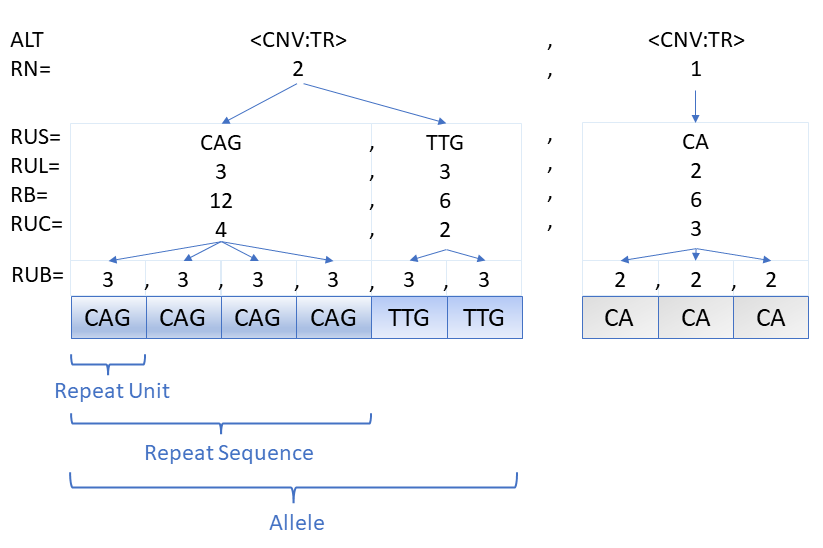
\includegraphics[width=4in,height=2.58in]{img/tandem_repeat_notation.png}
	\caption{$<$CNV:TR$>$ Tandem Repeats}
\end{figure}


A tandem repeat allele can be described by both a $<$CNV:TR$>$ 'summary' record as well as non-symbolic records.
When possible, these records should be phased with their corresponding $<$CNV:TR$>$ record as outlined in the following example.
In the following example, the reference genome contains a $(CAG)_{10}$ repeat at positions 101 to 130 inclusive, the first allele expands this to $(CAG)_{30}$ and the second allele is missing a $G$ from the 6th repeat unit $(CAG)_{5}(CA)_{1}(CAG)_{4}$:

\pagebreak
\footnotesize
\begin{landscape}
\begin{verbatim}
##fileformat=VCFv4.5
##INFO=<ID=SVLEN,Number=A,Type=Integer,Description="Length of structural variant">
##INFO=<ID=CN,Number=A,Type=Float,Description="Copy number of allele">
##INFO=<ID=RN,Number=A,Type=Integer,Description="Total number of repeat sequences in this allele">
##INFO=<ID=RUS,Number=.,Type=String,Description="Repeat unit sequence of the corresponding repeat sequence">
##INFO=<ID=RUL,Number=.,Type=Integer,Description="Repeat unit length of the corresponding repeat sequence">
##INFO=<ID=RUC,Number=.,Type=Float,Description="Repeat unit count of corresponding repeat sequence">
##INFO=<ID=RB,Number=.,Type=Integer,Description="Total number of bases in the corresponding repeat sequence">
##INFO=<ID=CIRUC,Number=.,Type=Float,Description="Confidence interval around RUC">
##INFO=<ID=CIRB,Number=.,Type=Integer,Description="Confidence interval around RB">
##INFO=<ID=RUB,Number=.,Type=Integer,Description="Number of bases in each individual repeat unit">
##FORMAT=<ID=GT,Number=1,Type=String,Description="Genotype">
##FORMAT=<ID=PS,Number=1,Type=Integer,Description="Phase set">
##FORMAT=<ID=CN,Number=1,Type=Float,Description="Copy number">
##ALT=<ID=CNV:TR,Description="Tandem repeat determined based on DNA abundance">
#CHROM POS ID REF ALT QUAL FILTER INFO FORMAT sample
chr1 100 cnv_notation T <CNV:TR>,<CNV:TR> . . SVLEN=30,30;CN=3,0.9666;RUS=CAG,CAG,CA,CAG;RN=1,3;RB=90,15,2,12  GT:PS:CN 1|2:100:3.9666
chr1 117 precise_alt2 AG A . . GT:PS 0|1:100
chr1 130 precise_alt1 G GCAGCAGCAGCAGCAGCAGCAGCAGCAGCAGCAGCAGCAGCAGCAGCAGCAGCAGCAGCAG . . GT:PS 1|0:100
\end{verbatim}
\end{landscape}
\pagebreak
\normalsize

Note the following:
\begin{itemize}
    \item As with all symbolic structural variant alleles, the POS of the $<$CNV:TR$>$ record is the base immediately preceding the tandem repeat
    \item The SVLEN of the $<$CNV:TR$>$ is the length of the reference allele.
    It is not the length of the $<$CNV:TR$>$ allele.
    \item The SVLEN of the $<$CNV:TR$>$ allele of a novel (with respect to the reference) tandem repeat should be 1.
    \item The POS of the $<$CNV:TR$>$ allele of a novel (with respect to the reference) tandem repeat should be the base immediately preceding the inserted tandem repeat sequence.
    \item Both a $<$CNV:TR$>$ and one or more non-symbolic records encoding the tandem repeat can be present.
    \item $<$CNV:TR$>$ and the non-symbolic records encoding the tandem repeat should be phased if possible.
    \item When both $<$CNV:TR$>$ and the equivalent non-symbolic records are present, the $<$CNV:TR$>$ should approximately encode the sequence but is not required to encode the sequence exactly.
	For example, SNVs and indels may be omitted in the $<$CNV:TR$>$ record.
    \item Variant callers which do not report allele-specific tandem repeats should use a single $<$CNV:TR$>$ ALT allele and the missing genotype for the GT field (for example, $./.$ if diploid).
    \item The INFO and FORMAT CN fields should be present for $<$CNV:TR$>$ records (as they are $<$CNV$>$ records) and, when present, must correspond to the sample allelic length divided by the reference allelic length.
	Note that CN FORMAT field represents the overall copy number and the INFO CN the allele-specific copy number.
    \item When benchmarking tandem repeats, the $<$CNV:TR$>$ interval provides a region over which a set of (preferably phased) non-symbolic records can be compared against for length and sequence composition.
    \item RN encodes the number of records for each allele in the RUS, RUL, RUC, RB fields.
	Conceptually, this a mechanism to encode a list-of-list with flat list format used in VCF.
    \item STRs should use RUS, whereas VNTRs should use RUL to ensure the VCF records are not excessively large.
    \item RUL should be omitted when RUS is present (as it is redundant when RS is present).
    \item RUS or RUL must be specified for each $<$CNV:TR$>$.
    \item Support for multiple levels of repeat nesting (such as STRs within VNTRs) is limited to the RUL repeat unit length field which allows the overall length of each top-level repeat unit to be encoded.
    \item The POS and SVLEN of $<$CNV:TR$>$ records should match the STR/VNTR reference catalog sizes for catalog-based callers.
    \item Variant normalisation has limited utility in regions of low complexity as almost identical haplotypes can have very different normalised representations.
\end{itemize}

In some cases, it is desirable to report the full repeat sequence of all alleles at a given repeat locus in a single VCF records.
There are no restrictions on doing so and in the above example, instead of reporting $precise\_alt1$ and $precise\_alt2$, the variants can be represented directly in a single record with a $REF$ of:
\scriptsize
\begin{verbatim}
CAGCAGCAGCAGCAGCAGCAGCAGCAGCAG
\end{verbatim}
\normalsize
and an $ALT$ of:
\scriptsize
\begin{verbatim}
CAGCAGCAGCAGCAGCAGCAGCAGCAGCAGCAGCAGCAGCAGCAGCAGCAGCAGCAGCAGCAGCAGCAGCAGCAGCAGCAGCAGCAGCAG,CAGCAGCAGCAGCAGCACAGCAGCAGCAG
\end{verbatim}
\normalsize

When the length or number of repeat units in a repeat sequence cannot be determined precisely, CIRB and/or CIRUC can be used to define the bounds.
For example, if the total number of $CAG$ repeats at the above locus was at least 50 ($(CAG)_{50-}$) and the mostly likely number of repeats was 65, then the $<$CNV:TR$>$ could be encoded as follows:

\footnotesize
\begin{verbatim}
chr1 100 . T <CNV:TR> . . SVLEN=30;CN=6.5;RUS=CAG;RUC=65;CIRUC=-15,. GT ./.
\end{verbatim}
\normalsize

Note that:
\begin{itemize}
	\item RN was omitted as it is only required if at least one $<$CNV:TR$>$ allele has RN greater than 1.
	\item The confidence interval bounds are relative to the nominal value.
	\item A missing upper bound indicates the maximum length is not known.
\end{itemize}

Exactly representing nested repeats results in the loss of some repeat information when representing with a $<$CNV:TR$>$ record.
For repeats such as $((ACCGGC)_{4}(ACCAGT))_{3-5}$, summarising the repeat structure in a $<$CNV:TR$>$ record requires either unrolling the inner repeats, or treating each outer repeat as a separate repeat sequence (the full repeat structure can be stored in a caller-specific non-standard INFO field).
For many VNTRs, the critical information to retain is the length of each repeat unit.
This length information can be encoded in the RUB field.
For example, a 10,000bp VNTRs domain repeated 5 times, each repeat 500bp longer than the previous can be encoded as follows:

\footnotesize
\begin{verbatim}
chr1 1000000 . T <CNV:TR> . . SVLEN=20000;CN=1.25;RUL=10000;RUC=5;RUB=10000,10500,11000,11500,12000 GT ./.
\end{verbatim}
\normalsize


	
	
\pagebreak
\section{BCF specification}

VCF is very expressive, accommodates multiple samples, and is widely used in the community.
Its biggest drawback is that it is big and slow.
Files are text and therefore require a lot of space on disk.
A normal batch of a hundred exomes is a few GB, but large-scale VCFs with thousands of exome samples quickly become hundreds of GBs.
Because the file is text, it is extremely slow to parse.

Overall, the idea behind is BCF2 is simple.
BCF2 is a binary, compressed equivalent of VCF that can be indexed with tabix and can be efficiently decoded from disk or streams.
For efficiency reasons BCF2 only supports a subset of VCF, in that all info and genotype fields must have their full types specified.
That is, BCF2 requires that if e.g.\ an info field {\tt AC} is present then it must contain an equivalent VCF header line noting that {\tt AC} is an allele indexed array of type integer.

\subsection{Overall file organization}

A BCF2 file is composed of a mandatory header, followed by a series of BGZF compressed blocks of binary BCF2 records.
The BGZF blocks allow BCF2 files to be indexed with tabix.

BGZF blocks are composed of a VCF header with a few additional records and a block of records.
Following the last BGZF BCF2 record block is an empty BGZF block (a block containing zero type of data), indicating that the records are done.

A BCF2 header follows exactly the specification as VCF, with a few extensions/restrictions:
\begin{itemize}
  \item All BCF2 files must have fully specified contigs definitions.
  No record may refer to a contig not present in the header itself.

  \item All INFO and GENOTYPE fields must be fully typed in the BCF2 header to enable type-specific encoding of the fields in records.
  An error must be thrown when converting a VCF to BCF2 when an unknown or not fully specified field is encountered in the records.
\end{itemize}

\subsection{Header}

The BCF2 header contains the following items:

\vspace{0.3cm}
{\small
\begin{tabular}{|l | l | p{30em} | } \hline
\textbf{Field} & \textbf{Type} & \textbf{Notes} \\ \hline
magic          & char[3]     & The characters ``{\tt BCF}'' \\ \hline
major\_version & uint8\_t    & 2 \\ \hline
minor\_version & uint8\_t    & 2 \\ \hline
l\_text        & uint32\_t   & Length of the ``text'' field, including the terminating NUL character \\ \hline
text           & char[l\_text] & VCF format header text, NUL-terminated \\ \hline
\end{tabular}}
\vspace{0.3cm}

The ``magic'' field and version numbers can be used to quickly examine the file to determine that it's a BCF2.2 file.
The ``text'' field contains the standard VCF header lines in text format, from \verb|##fileformat|
to \verb|#CHROM ...| inclusive, terminated by a NUL character.

Because the type is encoded directly in the header, the recommended extension for BCF2 formatted files is {\sl .bcf}.
BCF2 supports encoding values in a dictionary of strings.
The string map is provided by the keyword \verb|##dictionary=S0,S1,...,SN| as a comma-separate ordered list of strings.
See the ``Dictionary of strings'' section for more details.

\subsubsection{Dictionary of strings}

Throughout the BCF file most string values are be specified by integer reference to their dictionary values.
For example, the following VCF record:
\small
\begin{verbatim}
##INFO=<ID=ASP,Number=0,Type=Flag,Description="X">
##INFO=<ID=RSPOS,Number=1,Type=Integer,Description="Y">
##INFO=<ID=dbSNPBuildID,Number=1,Type=Integer,Description="Z">
##contig=<ID=20,length=62435964,assembly=B36,md5=f126cdf8a6e0c7f379d618ff66beb2da,species="Homo sapiens">
#CHROM POS ID REF ALT QUAL FILTER INFO
20 10144 rs144773400 TA T . PASS ASP;RSPOS=10145,dbSNPBuildID=134
20 10228 rs143255646 TA T . PASS ASP;RSPOS=10229;dbSNPBuildID=134
\end{verbatim}
\normalsize
would be encoded inline in BCF2 by reference to the relative position of the header line in the header (ASP=1, RSPOS=2, dbSNPBuildID=3, and PASS implicitly encoded in the first offset PASS=0).

\small
\begin{verbatim}
##INFO=<ID=ASP,Number=0,Type=Flag,Description="X">
##INFO=<ID=RSPOS,Number=1,Type=Integer,Description="Y">
##INFO=<ID=dbSNPBuildID,Number=1,Type=Integer,Description="Z">
##contig=<ID=20,length=62435964,assembly=B36,md5=f126cdf8a6e0c7f379d618ff66beb2da,species="Homo sapiens">
#CHROM POS ID REF ALT QUAL FILTER INFO
0 10144 rs144773400 TA T . s0 s1;s2=10145;s3=134
0 10228 rs143255646 TA T . s0 s1;s2=10229;s3=134
\end{verbatim}
\normalsize

Defined this way, the dictionary of strings depends on the order and the presence of all preceding header lines.
If an existing tag needs to be removed from a BCF, also all consequent tags throughout the whole BCF would have to be recoded.
In order to avoid this costly operation, a new IDX field can be used to explicitly define the position which is dropped on BCF-to-VCF conversion.
If not present, the implicit relative position is assumed.
If the IDX field is present in one record, it must be present also in all other dictionary-defining records.
The IDX tag is not necessary in newly created BCF files, but if present, the numbering must match the implicit dictionary of tags.

Note that the dictionary encoding has the magic prefix `s' here to indicate that the field's value is actually in the dictionary entry giving by the subsequent offset.
This representation isn't actually the one used in BCF2 records but it provides a clean visual guide for the above example.
Note also how the contig has been recoded as a offset into the list of contig declarations.

Note that ``PASS'' is always implicitly encoded as the first entry in the header dictionary.
This is because VCF allows FILTER fields to be PASS without explicitly listing this in the FILTER field itself.


\subsubsection{Dictionary of contigs}

The CHROM field in BCF2 is encoded as an integer offset into the list of \verb|##contig| field headers in the VCF header.
The offsets begin, like the dictionary of strings, at 0.
So for example if in BCF2 the contig value is 10, this indicates that the actual chromosome is the 11th element in the ordered list of \verb|##contig| elements.
Here's a more concrete example:

\small
\begin{verbatim}
##contig=<ID=20,length=62435964,assembly=B36,md5=f126cdf8a6e0c7f379d618ff66beb2da,species="Homo sapiens">
##contig=<ID=21,length=46944323,assembly=B36,md5=f1b74b7f9f4cdbaeb6832ee86cb426c6,species="Homo sapiens">
##contig=<ID=22,length=49691432,assembly=B36,md5=2041e6a0c914b48dd537922cca63acb8,species="Homo sapiens">
#CHROM POS ID REF ALT QUAL FILTER INFO
20 1 . T A . PASS .
21 2 . T A . PASS .
22 3 . T A . PASS .
\end{verbatim}
\normalsize

the actual CHROM field values in the encoded BCF2 records would be 0, 1, and 2 corresponding to the first (offset 0) \verb|##contig| element, etc.

\subsection{BCF2 records}

In BCF2, the original VCF records are converted to binary and encoded as BGZF blocks.
Each record is conceptually two parts.
First is the site information (chr, pos, INFO field).
Immediately after the sites data is the genotype data for every sample in the BCF2 file.
The genotype data may be omitted entirely from the record if there is no genotype data in the VCF file.
Compression of a BCF file is recommended but not required.

\subsubsection{Site encoding}
\label{BcfSiteEncoding}

{\small
\begin{tabular}{|l | l | p{30em} | } \hline
\textbf{Field} &	\textbf{Type} &	\textbf{Notes} \\ \hline
l\_shared & uint32\_t & Data length from CHROM to the end of INFO \\ \hline
l\_indiv  & uint32\_t & Data length of FORMAT and individual genotype fields \\ \hline
CHROM     & int32\_t  & Given as an offset into the mandatory contig dictionary \\ \hline
POS       & int32\_t  & 0-based leftmost coordinate \\ \hline
rlen      & int32\_t  & Length of the record as projected onto the reference sequence.
                        Must be the maximum of the length of the REF allele and the lengths
                        inferred from the SVLEN/LEN of any symbolic alleles \\ \hline
QUAL      & float     & Variant quality; 0x7F800001 for a missing value \\ \hline
n\_info   & uint16\_t & The number of INFO fields in this record \\ \hline
n\_allele & uint16\_t & The number of REF+ALT alleles in this record \\ \hline
n\_sample & uint24\_t & The number of samples in this record, stored as a \textbf{three} byte little-endian value.
                        Note that n\_sample must be equal to the number of samples in the header \\ \hline
n\_fmt    & uint8\_t  & The number of FORMAT keys.  See \ref{GenotypeEncoding} \\ \hline
ID       & typed string & Variant identifier; 0x07 for a missing value \\ \hline
REF+ALT  & list of n\_allele typed strings & the first allele is REF (mandatory) followed by n\_alleles - 1 ALT
                                             alleles, all encoded as typed strings \\ \hline
FILTER   & Typed vector of integers & a vector of integer offsets into dictionary, one for each FILTER field value.
                                      ``.'' is encoded as MISSING \\ \hline
INFO     & field key/value pairs & n\_info pairs of typed vectors.
                                   The first value must be a typed atomic integer giving the offset of the INFO field
                                   key into the dictionary.
                                   The second value is a typed vector giving the value of the field \\ \hline
Genotype values & see below & see below \\ \hline
\end{tabular}}

\subsubsection{Genotype encoding}
\label{GenotypeEncoding}

Genotype fields are encoded not by sample as in VCF but rather by field, with a vector of values for each sample following each field.
In BCF2, the following VCF line:

\vspace{0.3cm}
\begin{tabular}{l l l l}
FORMAT & NA00001 & NA00002 & NA00003 \\
GT:GQ:DP & 0/0:48:1 & 0/1:9:8 & 1/1:43:5 \\
\end{tabular}
\vspace{0.3cm}

would encoded as the equivalent of:

\vspace{0.3cm}
\begin{tabular}{l l l l}
GT=0/0,0/1,1/1 & GQ=48,9,43 & DP=1,8,5
\end{tabular}
\vspace{0.3cm}

Suppose there are i genotype fields in a specific record.
Each i is encoded by a triplet:

BCF2 site information encoding

\vspace{0.3cm}
\small
\begin{tabular}{ | p{2cm} | p{2.5cm} | p{9.5cm} | } \hline
Field & Type & Notes \\ \hline
fmt\_key & typed int & Format key as an offset into the dictionary \\ \hline
fmt\_type & uint8\_t+ & Typing byte of each individual value, possibly followed by a typed int for the vector length.  
In effect this is the same as the typing value for a single vector, but for genotype values it appears only once before the array of genotype field values \\ \hline
\makecell[tl]{fmt\_values \\ (by fmt type)} & Array of values & The information of each individual is concatenated in the vector.  Every value is of the same fmt type.
Variable-length vectors are padded with END\_OF\_VECTOR values; a string is stored as a vector of char \\  \hline
\end{tabular}
\normalsize
\vspace{0.3cm}

The value is always implicitly a vector of N values, where N is the number of samples.
The type byte of the value field indicates the type of each value of the N length vector.
For atomic values this is straightforward (size = 1).
But if the type field indicates that the values are themselves vectors (as often occurs, such as with the PL field) then each of the N values in the outer vector is itself a vector of values.
This encoding is efficient when every value in the genotype field vector has the same length and type.

It is recommended to respect the ordering as specified in the input VCF/BCF2 file, but parsers should not rely on a specific ordering.

If there are no sample records (genotype data) in this VCF/BCF2 file, the size of the genotypes block will be 0.


\subsubsection{Type encoding}
\label{BcfTypeEncoding}

In BCF2 values are all strongly typed in the file.
The type information is encoded in a prefix byte before the value, which contains information about the low-level type of the value(s) such as int32 or float, as well as the number of elements in the value.
The encoding is as follows:

\vspace{0.3cm}
\textbf{BCF2 type descriptor byte}

\vspace{0.3cm}
\begin{tabular}{|p{2cm} | p{10cm}|} \hline
Bit & Meaning \\ \hline
5,6,7,8 bits & The number of elements of the upcoming type. 
For atomic values, the size must be 1. 
If the size is set to 15, this indicates that the vector has 15 or more elements, and that the subsequent BCF2 byte stream contains a typed Integer indicating the true size of the vector. 
If the size is between 2--14, then this Integer is omitted from the stream and the upcoming stream begins immediately with the first value of the vector.
A size of 0 indicates that the value is MISSING. \\ \hline
1,2,3,4 bits & Type \\ \hline
\end{tabular}
\vspace{0.3cm}

The final four bits encodes an unsigned integer that indicates the type of the upcoming value in the data stream.

\textbf{BCF2 types}

\vspace{0.3cm}
\begin{tabular}{|l | l | l|} \hline
Lowest 4 bits & Hexadecimal encoding & Corresponding atomic type \\ \hline
0 & 0x00 & A MISSING value without an explicit type provided \\ \hline
1 & 0x?1 & Integer [8 bit] \\ \hline
2 & 0x?2 & Integer [16 bit] \\ \hline
3 & 0x?3 & Integer [32 bit] \\ \hline
5 & 0x?5 & Float [32 bit] \\ \hline
7 & 0x?7 & Character, ASCII encoded in 8 bits \\ \hline
\end{tabular}
\vspace{0.3cm}

In BCF2 strings are type=7 with an appropriate length.
Single characters are represented as strings with length=1.
Type codes 4,6,8--15 are reserved for future use.

\vspace{0.3cm}

\textbf{Integers} may be encoded as 8, 16, or 32 bit values, in little-endian order.
It is up to the encoder to determine the appropriate ranged value to use when writing the BCF2 file.
For integer types, the values 0x80, 0x8000, 0x80000000 are interpreted as missing values and 0x81, 0x8001, 0x80000001 as END\_OF\_VECTOR indicators (for 8, 16, and 32 bit values, respectively).
Note that the END\_OF\_VECTOR byte is not part of the vector itself and only END\_OF\_VECTOR bytes can follow.
In total, eight values are reserved for future use: 0x80--0x87, 0x8000--0x8007, 0x80000000--0x80000007.

\vspace{0.3cm}
\textbf{Floats} are encoded as single-precision (32 bit) in the basic format defined by the IEEE-754-1985 standard.
This is the standard representation for floating point numbers on modern computers, with direct support in programming languages like C and Java (see Java's Double class for example).
BCF2 supports the full range of values from -Infinity to +Infinity, including NaN.
BCF2 needs to represent missing values for single precision floating point numbers.
This is accomplished by writing the NaN value as the quiet NaN (qNaN), while the MISSING value is encoded as a signaling NaN.
From the NaN wikipedia entry, we have:

\begin{quote}
For example, a bit-wise example of a IEEE floating-point standard single precision (32-bit) NaN would be: s111 1111 1axx xxxx xxxx xxxx xxxx xxxx where s is the sign (most often ignored in applications), a determines the type of NaN, and x is an extra payload (most often ignored in applications).
If a = 1, it is a quiet NaN; if a is zero and the payload is nonzero, then it is a signaling NaN.
\end{quote}

\noindent A good way to understand these values is to play around with the IEEE encoder website.

\vspace{0.3cm}
\noindent Similarly to integers, the float value of 0x7F800001 is interpreted as a MISSING value and 0x7F800002 as the END\_OF\_VECTOR indicator. 
Note that the END\_OF\_VECTOR byte is not part of the vector itself and only END\_OF\_VECTOR bytes can follow.
In total, eight values are reserved for future use:


\vspace{0.1cm}
\begin{tabular}{| l | c | l |} \hline
\textbf{Value}   & \textbf{32-bit precision} & \textbf{Hexadecimal representation} \\ \hline
NaN	    & 0b0111 1111 1100 0000 0000 0000 0000 0000 & 0x7FC00000 \\ \hline
MISSING & 0b0111 1111 1000 0000 0000 0000 0000 0001 & 0x7F800001 \\ \hline
END\_OF\_VECTOR & 0b0111 1111 1000 0000 0000 0000 0000 0010 & 0x7F800002 \\ \hline
reserved & 0b0111 1111 1000 0000 0000 0000 0000 0011 & 0x7F800003 \\ \hline
$\ldots$ & $\ldots$ & $\ldots$ \\ \hline
reserved & 0b0111 1111 1000 0000 0000 0000 0000 0111 & 0x7F800007 \\ \hline
\end{tabular}

\vspace{0.3cm}
\textbf{Character} values are not explicitly typed in BCF2.
Instead, VCF Character values must be encoded by a single character string. See also \ref{character-encoding}.

\vspace{0.3cm}
\textbf{Flags} values --- which can only appear in INFO fields --- in BCF2 should be encoded by any non-reserved value.
The recommended best practice is to encode the value as an 1-element INT8 (type 0x11) with value of 1 to indicate present.
Because FLAG values can only be encoded in INFO fields, BCF2 provides no mechanism to encode FLAG values in genotypes, but could be easily extended to do so if allowed in a future VCF version.

\vspace{0.3cm}
\textbf{String} values have two basic encodings.
For INFO, FORMAT, and FILTER keys these are encoded by integer offsets into the header dictionary.
For string values, such as found in the ID, REF, ALT, INFO, and FORMAT fields, strings are encoded as typed array of ASCII encoded bytes.
The array isn't terminated by a NUL byte.
The length of the string is given by the length of the type descriptor.

Suppose you want to encode the string ``{\tt ACAC}''.
First, we need the type descriptor byte, which is the string type 0x07 or'd with inline size (4) yielding the type byte of 0x40 $|$ 0x07 = 0x47.
Immediately following the type byte is the four byte ASCII encoding of ``{\tt ACAC}'': 0x41 0x43 0x41 0x43.
So the final encoding is:

\vspace{0.1cm}
\begin{tabular}{| l | l |} \hline
0x47 0x41 0x43 0x41 0x43 & String type with inline size of 4 followed by ACAC in ASCII \\ \hline
\end{tabular}
\vspace{0.3cm}

Suppose you want to encode the string ``{\tt VariantCallFormatSampleText}'', a string of size 27.
First, we need the type descriptor byte, which is the string type 0x07.
Because the size exceeds the inline size limit ($27 \geq 15$) we set the size to overflow, yielding the type byte of 0xF0 $|$ 0x07 = 0xF7.
Immediately following the type byte is the typed size of 27, which we encode by the atomic INT8 value: 0x11 followed by the actual size 0x1B.
Finally comes the actual bytes of the string: 0x56 0x61 0x72 0x69 0x61 0x6E 0x74 0x43 0x61 0x6C 0x6C 0x46 0x6F 0x72 0x6D 0x61 0x74 0x53 0x61 0x6D 0x70 0x6C 0x65 0x54 0x65 0x78 0x74.
So the final encoding is:

\vspace{0.3cm}
\begin{tabular}{ | p{9cm} | p{6cm} | } \hline
0xF7 & string with overflow size \\ \hline
0x11 0x1B & overflow size encoded as INT8 with value 27 \\ \hline
0x56 0x61 0x72 0x69 0x61 0x6E 0x74 0x43 0x61 0x6C 0x6C 0x46 0x6F 0x72 0x6D 0x61 0x74 0x53 0x61 0x6D 0x70 0x6C 0x65 0x54 0x65 0x78 0x74 & message in ASCII \\ \hline
\end{tabular}
\vspace{0.3cm}

Suppose you want to encode the missing value `.'.
This is simply a string of size 0 = 0x07.

\vspace{0.3cm}
In VCF there are sometimes fields of type list of strings, such as a number field of unbounded size encoding the amino acid changes due to a mutation.
Since BCF2 doesn't directly support vectors of strings (a vector of character is already a string) we collapse the list of strings into a single comma-separated string, encode it as a regular BCF2 vector of characters, and on reading explode it back into the list of strings.
This works because strings in VCF cannot contain `{\tt ,}' (it's a field separator) and so we can safely use `{\tt ,}' to separate the individual strings.

% String vectors in BCF do not need to start with comma, as the number of
% values is indicated already in the definition of the tag in the header.
%
% For efficiency
% reasons we put a comma at the start of the collapsed string, so that just the
% first character can be examined to determine if the string is collapsed.
%END\_OF\_VECTOR
% To be concrete, suppose we have a info field around X=[A,B,C,D].  This is
% encoded in BCF2 as a single string ``,A,B,C,D'' of size 8, so it would have
% type byte 0x87 followed by the ASCII encoding 0x2C 0x41 0x2C 0x42 0x2C 0x43
% 0x2C 0x44.

\vspace{0.3cm}

\textbf{Vectors} --- The BCF2 type byte may indicate that the upcoming data stream contains not a single value but a fixed length vector of values.
The vector values occur in order (1st, 2nd, 3rd, etc) encoded as expected for the type declared in the vector's type byte.
For example, a vector of 3 16-bit integers would be laid out as first the vector type byte, followed immediately by 3 2-byte values for each integer, including a total of 7 bytes.

Missing values in vectors are handled slightly differently from atomic values.
There are two possibilities for missing values:

One (or more) of the values in the vector may be missing, but others in the vector are not.
Here each value should be represented in the vector, and each corresponding BCF2 vector value either set to its present value or the type equivalent MISSING value.
Alternatively the entire vector of values may be missing.
In this case the correct encoding is as a type byte with size 0 and the appropriate type MISSING.
Suppose we are encoding the record ``AC=[1,2,3]'' from the INFO field.
The AC key is encoded in the standard way.
This would be immediately followed by a typed 8-bit integer vector of size 3, which is encoded by the type descriptor 0x31.
The type descriptor is immediately followed by the three 8-bit integer values: 0x01 0x02 0x03, for a grand total of 4 bytes: 0x31010203.

Suppose we are at a site with many alternative alleles so AC=[1,2,3,4,5,6,7,8,9,10,11,12,13,14,15,16].
Since there are 16 values, we have to use the long vector encoding.
The type of this field is 8 bit integer with the size set to 15 to indicate that the size is the next stream value, so this has type of 0xF1.
The next value in the stream is the size, as a typed 8-bit atomic integer: 0x11 with value 16 0x10.
Each integer AC value is represented by it's value as a 8 bit integer.
The grand total representation here is:

\vspace{0.3cm}
\begin{tabular}{|p{9cm} | p{6cm}|} \hline
0xF1 0x01 0x10 & 8 bit integer vector with overflow size \\ \hline
0x01 0x02 0x03 0x04 0x05 0x06 0x07 0x08 0x09 0x0A 0x0B 0x0C 0x0D 0x0E 0x0F 0x10 & 1--16 as hexadecimal 8 bit integers \\ \hline
\end{tabular}
\vspace{0.3cm}

Suppose this INFO field contains the ``AC=.'', indicating that the AC field is missing from a record with two alt alleles.
The correct representation is as the typed pair of AC followed by a MISSING vector of type 8-bit integer: 0x01.

\vspace{0.3cm}
\textbf{Vectors of mixed length} --- In some cases genotype fields may be vectors whose length differs among samples.  
For example, some CNV call sets encode different numbers of genotype likelihoods for each sample, given the large number of potential copy number states, rather padding all samples to have the same number of fields.  
For example, one sample could have CN0:0,CN1:10 and another CN0:0,CN1:10,CN2:10.  
In the situation when a genotype field contain vector values of different lengths, these are represented in BCF2 by a vector of the maximum length per sample, with all values in the each vector aligned to the left, and END\_OF\_VECTOR values assigned to all values not present in the original vector.  
The BCF2 encoder / decoder must automatically add and remove these END\_OF\_VECTOR values from the vectors. Note that the use of END\_OF\_VECTOR means that it is legal to encode a vector VCF field with MISSING values.

For example, suppose I have two samples, each with a FORMAT field X.  
Sample A has values [1], while sample B has [2,3].  
In BCF2 this would be encoded as [1, END\_OF\_VECTOR] and [2, 3]. 
Diving into the complete details, suppose X is at offset 3 in the dictionary, which is encoded by the typed INT8 descriptor 0x11 followed by the value 0x03. 
Next we have the type of the each format field, which here is a 2 element INT8 vector: 0x21.  
Next we have the encoding for each sample, A = 0x01 0x81 followed by B = 0x02 0x03.  
All together we have:

\vspace{0.3cm}
\begin{tabular}{|p{2cm} | l |} \hline
0x11 0x03 & X dictionary offset \\ \hline
0x21 & each value is a 2 element INT8 value \\ \hline
0x01 0x81 & A is [1, END\_OF\_VECTOR] \\ \hline
0x02 0x03 & B is [2, 3] \\ \hline
\end{tabular}
\vspace{0.3cm}


\vspace{0.3cm}
A \textbf{Genotype (GT) field} is encoded in a typed integer vector (can be 8, 16, or even 32 bit if necessary) with the number of elements equal to the maximum ploidy among all samples at a site.
For one individual, each integer in the vector is organized as $(allele+1) << 1 \mid phased$ where allele is set to $-1$ if the allele in GT is a dot `.' (thus the higher bits are all 0).
The vector is padded with the END\_OF\_VECTOR values if the GT having fewer ploidy.
We note specifically that except for the END\_OF\_VECTOR byte, no other negative values are allowed in the GT array.
When processing VCF version 4.3 or earlier files, the phasing of the first allele should be treated as missing and inferred from the remaining alleles.

Examples:

\vspace{0.3cm}
\small
\begin{tabular}{|p{2.5cm} | p{10cm} | p{3cm}|} \hline
0/1 & in standard format $(0 + 1) << 1 \mid 0$ followed by $(1 + 1) << 1 \mid 0$ & 0x02 04 \\ \hline
0/1, 1/1, and 0/0 & three samples encoded consecutively & 0x02 04 04 04 02 02 \\ \hline
$0\mid1$ & $(1 + 1) << 1 \mid 1$ = 0x05 preceded by the standard first byte value 0x02 & 0x02 05 \\ \hline
./. & where both alleles are missing & 0x00 00 \\ \hline
0 & as a haploid it is represented by a single byte & 0x02 \\ \hline
1 & as a haploid it is represented by a single byte & 0x04 \\ \hline
0/1/2 & is tetraploid, with alleles & 0x02 04 06 \\ \hline
$0/1\mid2$ & is tetraploid with a single phased allele & 0x02 04 07 \\ \hline
0 and 0/1 & pad out the final allele for the haploid individual & 0x02 81 02 04\\ \hline
\end{tabular}
\normalsize

\vspace{0.3cm}
The final example is something seen on chrX when we have a haploid male and a diploid female.
The male genotype vector is terminated prematurely by the END\_OF\_VECTOR value.
\vspace{0.3cm}


\subsection{Encoding a VCF record example}

Let's encode a realistic (but made-up) VCF record.
This is a A/C SNP in HM3 (not really) called in~3 samples.
In this section we'll build up the BCF2 encoding for this record.
\scriptsize
\begin{verbatim}
#CHROM POS ID REF ALT QUAL FILTER INFO FORMAT NA00001 NA00002 NA00003
chr1 101 rs123 A C 30.1 PASS HM3;AC=3;AN=6;AA=C GT:GQ:DP:AD:PL 0/0:10:32:32,0:0,10,100 0/1:10:48:32,16:10,0,100 1/1:10:64:0,64:100,10,0
\end{verbatim}
\normalsize

\subsubsection{Encoding CHROM and POS}

First, let's assume that {\tt chr1} is the second chromosome to appear in the contig list---right after {\tt chrM} ({\tt MT}).
So its offset is 1.
The {\tt POS} BCF2 field value is~101 (obviously).
Because these are both typed values in the BCF2 record, we encode both in their most compact 8-bit value form.
The type byte for an atomic 8-bit integer is 0x11.
The value for the contig offset is 1 = 0x01.
The value 101 is encoded as the single byte 0x65.
So in total these are represented as:

\vspace{0.3cm}
\begin{tabular}{|l | l|} \hline
0x01000000 & CHROM offset is at 1 in 32 bit little endian \\ \hline
0x64000000 & POS in 0 base 32 bit little endian \\ \hline
0x01000000 & rlen = 1 (it's just a SNP) \\ \hline
\end{tabular}

\subsubsection{Encoding QUAL}

The QUAL field value is 30.1, which we encode as an untyped single precision 32-bit float:

\vspace{0.3cm}
\begin{tabular}{|l| l|} \hline
0x41 0xF0 0xCC 0xCD & QUAL = 30.1 as 32-bit float \\ \hline
\end{tabular}

\subsubsection{Encoding ID}

This ID value is a 5-element string, so is encoded as type descriptor 0x57 followed by the five bytes for the string of {\tt 0x72 0x73 0x31 0x32 0x33}.
The full encoding is:

\vspace{0.3cm}
\begin{tabular}{|l| l|} \hline
0x57 0x72 0x73 0x31 0x32 0x33 & ID = rs123 \\ \hline
\end{tabular}

\subsubsection{Encoding REF/ALT fields}

We encode each of REF and ALT as typed strings, first REF followed immediately by ALT.
Each is a 1 element string (0x17), which would then be followed by the single bytes for the bases of 0x43 and 0x41:

\vspace{0.3cm}
\begin{tabular}{|l| l|} \hline
0x17 0x41 & REF A \\ \hline
0x17 0x43 & ALT C \\ \hline
\end{tabular}

\vspace{0.3cm}
Just for discussion, suppose instead that ALT was ALT=C,T.
The only thing that could change is that there would be another typed string following immediately after C encoding 0x17 (1 element string) with the value of 0x54.

\subsubsection{Encoding FILTER}

``PASS'' is implicitly encoded as the first entry in the header dictionary (see dictionary of strings).
Here we encode the PASS FILTER field as a vector of size 1 of type 8-bit, which has type byte is 0x11.
The value is the offset 0:

\vspace{0.3cm}
\begin{tabular}{|l| l|} \hline
0x11 0x00 & FILTER field PASS \\ \hline
\end{tabular}

\subsubsection{Encoding the INFO fields}

HM3;AC=3;AN=6;AA=C
Let's assume that the header dictionary elements for HM3, AC, AN, and AA are at 80, 81, 82, and 83 respectively.
All of these can be encoded by 1-element INT8 values (0x11), with associated hex values of 0x50, 0x51, 0x52, and 0x53 respectively.

First is HM3.
The entry begins with the key: 0x11 0x50.
The HM3 field is a flag with no associated value and therefore the rest of the entry is the special case of a missing value without an explicit type provided.
Altogether we have:

\vspace{0.3cm}
\begin{tabular}{|l| l|} \hline
0x11 0x50 0x00 & HM3 flag is present \\ \hline
\end{tabular}
\vspace{0.3cm}

Now let's encode the two atomic 8-bit integer fields AC and AN:

\vspace{0.3cm}
\begin{tabular}{|l| l|} \hline
0x11 0x51 & AC key \\ \hline
0x11 0x03 & with value of 3 \\ \hline
0x11 0x52 & AN key \\ \hline
0x11 0x06 & with value of 6 \\ \hline
\end{tabular}
\vspace{0.3cm}

The ancestral allele (AA) tell us that among other primates the original allele is C, a Character here.
Because we represent Characters as single element strings in BCF2 (0x17) with value 0x43 (C).
So the entire key/value pair is:

\vspace{0.3cm}
\begin{tabular}{|l |l|} \hline
0x11 0x53 & AA key \\ \hline
0x17 0x43 & with value of C \\ \hline
\end{tabular}

\subsubsection{Encoding Genotypes}

Continuing with our example:

\vspace{0.3cm}
\begin{tabular}{l l l l}
FORMAT & NA00001 & NA00002 & NA00003 \\
GT:GQ:DP:AD:PL & 0/0:10:32:32,0:0,10,100 & 0/1:10:48:32,16:10,0,100 & 1/1:10:64:0,64:100,10,0 \\
\end{tabular}
\vspace{0.3cm}

Here we have the specially encoded GT field.
We have two integer fields GQ and DP.
We have the AD field, which is a vector of 2 values per sample.
And finally we have the PL field which is 3 values per sample.
Let's say that the FORMAT keys for GT, GQ, DP, AD, and PL are at offsets 1, 2, 3, and 4, 5, respectively.
Now let's encode each of the genotype fields in order of the VCF record (GT, GQ, DP, AD, and then PL):

GT triplet begins with the key: 0x1101.
Next is the type of the field, which will be a 2-element (diploid) INT8 type: 0x21.
This is followed by 3 2-byte arrays of values 0x0202 0x0204 0x0404 (see genotype encoding example for details).
The final encoding is 0x1101 0x21 0x020202040404

GQ triplet begins with the key 0x1102.
Because these values are small, we encode them as 8 bit atomic integers with type code 0x11.
As each value is the same (10 = 0x0A) the GQ field is encoded as 0x1102 0x11 0x0A0A0A

DP almost identical to GQ.
First is the 0x1103 key, followed by 3 8-bit atomic integers encoded as 0x11 (the type) 0x20 (DP=32), 0x30 (DP=48) and 0x40 (DP=64).
So we have: 0x1103 0x11203040

AD is more complex.
The key is simple, just like the others, with 0x1104.
Because the AD field is a vector of 2 values for each genotype, the value of key/value pair a vector type.
Because the integer values in each AD field of each sample are small they are encoded by 8 bit values.
So the value type is = 0x21.
For sample one there are two values: 32,0 which are 0x30 and 0x00.
Samples two and three are 0x30 0x20 and 0x00 0x40 respectively.
So ultimately this field is encoded as 0x1104 0x21 0x300030200040

PL is just like AD but with three values per sample.
The key is 0x1105.
Because the PL field is a vector of 3 values for each genotype, the value of key/value pair a vector type, and because the size is 3 it's encoded in the size field of the type.
Again, because the integer values in each PL field of each sample are small they are encoded by 8 bit values.
So the value type 0x31.
For sample one there are three values: 0, 10, and 100 which are 0x00, 0x0A, and 0x64.
Samples two and three have the same values but in a slightly different order.
So ultimately the PL field is encoded as 0x1105 0x31 0x000A64 0x0A0064 0x640A00

So the genotype block contains:

\vspace{0.3cm}
\begin{tabular}{|l| l|} \hline
0x1101 0x21 0x020202040404 & GT \\ \hline
0x1102 0x11 0x0A0A0A & GQ \\ \hline
0x1103 0x11 0x203040 & DP \\ \hline
0x1104 0x21 0x300030200040 & AD \\ \hline
0x1105 0x31 0x000A640A0064640A00 & PL \\ \hline
\end{tabular}
\vspace{0.3cm}

\textbf{Putting it all together}

We need to determine a few values before writing out the final block:

l\_shared = 51 (Data length from CHROM to the end of INFO)

l\_indiv = 42 (Data length of FORMAT and individual genotype fields)

n\_info = 4 (Number of INFO fields)

n\_allele = 2 (Number of alleles, including REF)

n\_sample = 3 (Number of samples)

n\_fmt = 5 (Number of FORMAT keys)

\vspace{0.3cm}
\begin{tabular}{|l| l|} \hline
0x33000000 & l\_shared as 32-bit little endian hex \\ \hline
0x2A000000 & l\_indiv as 32-bit little endian hex \\ \hline
0x01000000 & CHROM offset is at 1 in 32 bit little endian \\ \hline
0x64000000 & POS in 0-based 32-bit little endian \\ \hline
0x01000000 & rlen = 1 (it's just a SNP) \\ \hline
0x41 0xF0 0xCC 0xCD & QUAL = 30.1 as 32-bit float \\ \hline
0x0400     & n\_info as 16-bit little-endian \\ \hline
0x0200     & n\_allele as 16-bit little-endian \\ \hline
0x030000   & n\_sample as 24-bit little-endian \\ \hline
0x05       & n\_fmt \\ \hline
0x57 0x72 0x73 0x31 0x32 0x33 & ID = rs123 \\ \hline
0x17 0x41 & REF A \\ \hline
0x17 0x43 & ALT C \\ \hline
0x11 0x00 & FILTER field PASS \\ \hline
0x11 0x50 0x00 & HM3 flag is present \\ \hline
0x11 0x51 & AC key \\ \hline
0x11 0x03 & with value of 3 \\ \hline
0x11 0x52 & AN key \\ \hline
0x11 0x06 & with value of 6 \\ \hline
0x11 0x53 & AA key \\ \hline
0x17 0x43 & with value of C \\ \hline
0x1101 0x21 0x020202040404 & GT \\ \hline
0x1102 0x11 0x0A0A0A & GQ \\ \hline
0x1103 0x11 0x203040 & DP \\ \hline
0x1104 0x21 0x300030200040 & AD \\ \hline
0x1105 0x31 0x000A640A0064640A00 & PL \\ \hline
\end{tabular}
\vspace{0.3cm}

That's quite a lot of information encoded in only 96 bytes!

\subsection{BCF2 block gzip and indexing}

These raw binary records may be subsequently encoded into BGZF blocks following the BGZF compression format, section 3 of the SAM format specification.
BCF2 records can be raw, though, in cases where the decoding/encoding costs of bgzipping the data make it reasonable to process the data uncompressed, such as streaming BCF2s through pipes with samtools and bcftools.
Here the files should be still compressed with BGZF but with compression 0.
Implementations should perform BGZF encoding and must support the reading of both raw and BGZF encoded BCF2 files.

BCF2 files are expected to be indexed through the same index scheme, section~4 as BAM files and other block-compressed files with BGZF.

\section{List of changes}

\subsection{Changes between VCFv4.5 and VCFv4.4}

\begin{itemize}
	\item Added Number=P support for fields with cardinality matching sample ploidy/local copy number.
	\item Added local allele support (Number=LOCAL-A, LOCAL-G, LOCAL-R; FORMAT LA, LAD, LADF, LADR, LEC, LGL, LGP, LGT, LPL, LPP) to reduce the size of multi-sample VCFs and enable lossless merging.
	\item Deprecated INFO END. It is now a computed field written only for backwards compatibility with older versions of VCF.
	\item Added FORMAT LEN to support sample-specific $<$*$>$ alleles.
\end{itemize}

\subsection{Changes between VCFv4.4 and VCFv4.3}

\begin{itemize}
\item Added tandem repeat support ($<$CNV:TR$>$, RN, RUS, RUL, RB, CIRB, RUC, CIRUC, RUB)
\item Redefined INFO CN as allele-specific copy number and FORMAT CN as total copy number.
\item Redefined INFO and FORMAT CN to support non-integer copy numbers.
\item Added support for phasing and derivative chromosome reconstruction in the presence of SVs (PSL, PSO, PSQ)
\item Added SVCLAIM to disambiguate copy number based $<$DEL$>$ and $<$DUP$>$ variants from breakpoint based ones.
\item Conceptually separated variant detection and interpretation.
\item Added EVENTTYPE/EVENT to enable the multiple records encoding complex genomic rearrangements to be grouped together.
\item Added polyploid partial phasing support (e.g. GT $|0|0/1/2$). GT now defined as a prefix notation with the first phasing indicator optional.
\item Redefined $Number=$ for SVLEN, CIPOS, CIEND, HOMLEN, HOMSEQ, BKPTID, MEINFO, METRANS, DGVID, DBVARID, DBRIPID, MATEID, PARID, EVENT, CN, CICN to support multiple symbolic alleles.
\item Redefined END as the end position of the longest ALT allele. Note that END remains $Number=1$.
\item Redefined SVLEN to always be positive and be meaningful for INV variants.
\item Redefined SVLEN, END and BCF rlen to support both $<*>$ and symbolic structural variant alleles in the same record.
\item Number, Type and Description required only for INFO meta-information lines
\item Clarified CIPOS should be used to define micro-homology bounds
\item Clarified INFO lines field ordering
\item Clarified that symbolic and breakpoint notation ALT alleles are case sensitive.
\item Deprecated SVTYPE
\item Removed DPADJ, CNADJ, CICNADJ
\item Disallowed BND ALT records (these should use breakpoint notation anyway)
\item Removed definition of DP from Section 3 as it was already defined in Section 1.6.1.8.
\item Deprecated bundles in favour of PSL-based phasing.
\item Updated SV examples.
\item BCF parsers should perform BGZF encoding and must support both raw and BGZF encoded files.
\end{itemize}

\subsection{Changes to VCFv4.3}

\begin{itemize}
\item More strict language: ``should'' replaced with ``must'' where appropriate
\item Tables with Type and Number definitions for INFO and FORMAT reserved keys

\item
The set of characters allowed in VCF contig names is now the same as that allowed in SAM reference sequence names, which was restricted in January 2019.
The characters `{\tt\verb|\|\,,\,"`'\,()\,\verb|{}|}' are now invalid in VCF contig names, while `{\tt *}' is now valid when not the first character.
(The characters `{\tt []\,<>}' and initial~`{\tt *}'/`{\tt =}' were already invalid and remain so.)

The VCF specification previously disallowed colons (`{\tt :}') in contig names to avoid confusion when parsing breakends, but this was unnecessary.
Even with contig names containing colons, the breakend mate position notation can be unambiguously parsed because the ``{\tt :}\emph{pos}'' part is \textbf{always} present.
\item Added PP tag which is the phred-scaled analogue to GP
\end{itemize}

\subsection{Changes between VCFv4.2 and VCFv4.3}

\begin{itemize}
\item VCF compliant implementations must support both LF and CR+LF newline conventions
\item INFO and FORMAT tag names must match the regular expression \texttt{\^{}[A-Za-z\_][0-9A-Za-z\_.]*\$}
\item Spaces are allowed in INFO field values
\item Characters with special meaning (such as `;' in INFO, `:' in FORMAT, and `\%' in both) can be encoded using percent encoding (see Section~\ref{character-encoding})
\item The character encoding of VCF files is UTF-8.
\item The SAMPLE field can contain optional DOI URL for the source data file
\item Introduced \#\#META header lines for defining phenotype metadata
\item New reserved tag ``CNP'' analogous to ``GP'' was added. Both CNP and GP use 0 to 1 encoding, which is a change from previous phred-scaled GP.
\item In order for VCF and BCF to have the same expressive power, we state explicitly that Integers and Floats are 32-bit numbers.
Integers are signed.
\item We state explicitly that zero length strings are not allowed, this includes the CHROM and ID column, INFO IDs, FILTER IDs and FORMAT IDs.
Meta-information lines can be in any order, with the exception of \#\#fileformat which must come first. 
\item All header  lines of the form \#\#key=$<$ID=xxx,...$>$ must have an ID value that is unique for a given value of ``key''.
All header lines whose value starts with ``$<$'' must have an ID field.
Therefore, also \#\#PEDIGREE newly requires a unique ID.
\item We state explicitly that duplicate IDs, FILTER, INFO or FORMAT keys are not valid.
\item A section about gVCF was added, introduced the $<$*$>$ symbolic allele.
\item A section about tag naming conventions was added.
\item New reserved AD, ADF, and ADR INFO and FORMAT fields added.
\item Removed unused and ill-defined GLE FORMAT tag.
\item Chromosome names cannot use reserved symbolic alleles and contain characters used by breakpoints (Section~\ref{sec-contig-field}).
\item IUPAC ambiguity codes should be converted to a concrete base.
\item Symbolic ALTs for IUPAC codes.
\end{itemize}

\subsection{Changes between BCFv2.1 and BCFv2.2}
\begin{itemize}
\item BCF header lines can include optional IDX field
\item We introduce END\_OF\_VECTOR byte and reserve 8 values for future use
\item Clarified that except the END\_OF\_VECTOR byte, no other negative values are allowed in the GT array 
\item String vectors in BCF do not need to start with comma, as the number of values is indicated already in the definition of the tag in the header.
\item The implicit filter PASS was described inconsistently throughout BCFv2.1: It is encoded as the first entry in the dictionary, not the last.
\end{itemize}

\subsection{Changes between VCFv4.1 and VCFv4.2}
\begin{itemize}
\item In the HEADER the INFO definition allow additional field after the 4 first mandatory fields
\item INFO fields definition can use Number=R to specify one per allele including the reference.
\item Allow star allele in the ALT for describing upstream deletion
\end{itemize}

\end{document}
